\documentclass[UTF8,12pt]{ctexbook}

\usepackage[]{ctex}
\usepackage{amsmath,amsthm,amsfonts,amssymb}
\usepackage{geometry}
\usepackage[colorlinks=true]{hyperref}
\usepackage{indentfirst}
\usepackage[center]{titlesec}
\usepackage{graphicx}
\usepackage{esint}
\usepackage{cases}
\usepackage{tikz}
\usepackage{tikz-3dplot}
\usepackage{pgfplots}
\usepackage{listings}
\usepackage{multicol}
\usepackage{multirow}
\usepackage{pdfpages}
\usepackage{cancel}
\usepackage{markdown}

\usetikzlibrary{svg.path}
\usetikzlibrary{positioning}
\usetikzlibrary{intersections}

\geometry{left=1cm,right=1cm,top=3cm,bottom=3cm}
\title{db的日常笔记}
\date{最后编译日期:\today}
\author{dbydd}
\kaishu
\setlength{\parindent}{2em}
\titleformat{\section}[block]{\LARGE\itshape\mdseries}{\arabic{section}}{1em}{}[]
\titleformat{\subsection}[block]{\Large\itshape\mdseries}{\arabic{section}.\arabic{subsection}}{1em}{}[]
\titleformat{\subsubsection}[block]{\large\itshape\mdseries}{\arabic{section}.\arabic{subsection}.\arabic{subsubsection}}{1em}{}[]
\titleformat{\paragraph}[block]{\small\bfseries}{[\arabic{paragraph}]}{1em}{}[]
\setcounter{secnumdepth}{3}
\setcounter{tocdepth}{3}

\lstloadlanguages{C,C++,csh,Java,Python}

  \lstset{ %
    % language=csh,                % the language of the code
    basicstyle=\footnotesize,           % the size of the fonts that are used for the code
    numbers=left,                   % where to put the line-numbers
    numberstyle=\tiny\color{gray},  % the style that is used for the line-numbers
    stepnumber=2,                   % the step between two line-numbers. If it's 1, each line 
                                    % will be numbered
    numbersep=5pt,                  % how far the line-numbers are from the code
    backgroundcolor=\color{white},      % choose the background color. You must add \usepackage{color}
    showspaces=false,               % show spaces adding particular underscores
    showstringspaces=false,         % underline spaces within strings
    showtabs=false,                 % show tabs within strings adding particular underscores
    frame=single,                   % adds a frame around the code
    rulecolor=\color{black},        % if not set, the frame-color may be changed on line-breaks within not-black text (e.g. commens (green here))
    tabsize=2,                      % sets default tabsize to 2 spaces
    captionpos=b,                   % sets the caption-position to bottom
    breaklines=true,                % sets automatic line breaking
    breakatwhitespace=false,        % sets if automatic breaks should only happen at whitespace
    title=\lstname,                 % show the filename of files included with \lstinputlisting;
                                    % also try caption instead of title
    keywordstyle=\color{blue},          % keyword style
    commentstyle=\color{dkgreen},       % comment style
    stringstyle=\color{mauve},         % string literal style
    escapeinside={\%*}{*)},            % if you want to add LaTeX within your code
    % morekeywords={*,...}               % if you want to add more keywords to the set
  }

  \renewcommand{\qed}{\rightline{\qedsymbol-Q.E.D.(Quod Erat Demonstrandum/证毕)}}

\newcommand{\limNormal}[1]{\lim\limits_{#1}}
\newcommand{\myLimToZero}{\limNormal{x \to 0}}
\newcommand{\myLimToInf}{\limNormal{x \to \infty}}
\newcommand{\derivative}{^\prime}
\newcommand{\doubleDerivative}{^{\prime\prime}}
\newcommand{\tripleDerivative}{^{\prime\prime\prime}}
\newcommand{\aLotDerivative}[1]{^{(#1)}}
\newcommand{\partialDerivative}[1]{^\prime_{#1}}
\newcommand{\mathCombination}[2]{C_{#1}^{#2}}
\newcommand{\mathPermutation}[2]{P_{#1}^{#2}}
\newcommand{\upDownSum}[2]{\sum\limits_{#2}^{#1}}
\newcommand{\upDownProd}[2]{\prod\limits_{#2}^{#1}}
\newcommand{\updownUnion}[2]{\bigcup\limits_{#2}^{#1}}
\newcommand{\updownIntersection}[2]{\bigcap\limits_{#2}^{#1}}
\newcommand{\fDerivative}[1]{\fint\derivative(#1)}
\newcommand{\defFunction}[1]{f(#1)}
\newcommand{\definiteIntegral}[2]{\int^{#1}_{#2}}
\newcommand{\mathConstant}{\mathbb{C}}
\newcommand{\degree}{^\circ}
\newcommand{\projection}[1]{Prj_{#1}}
\newcommand{\bigCase}[1]{\left(#1\right)}
\newcommand{\dependent}[1]{\langle#1\rangle}
\newcommand{\innerProduct}[2]{\dependent{#1,#2}}
\newcommand{\transpose}{^T}
\newcommand{\spaceline}{\\\indent}
\newcommand{\directionDerivative}[3]{\left.\cfrac{\partial #1}{\partial #2}\right|_{#3}}
\newcommand{\partialDerivativeFrac}[2]{\cfrac{\partial #1}{\partial #2}}
\newcommand{\doubleIntegralOnZone}[1]{\iint\limits_{#1}}
\newcommand{\defDoubleIntegralOnZone}[3]{{\iint\limits_{#1}}^{#2}_{#3}}
\newcommand{\defTripleIntegralOnZone}[3]{{\iiint\limits_{#1}}^{#2}_{#3}}
\newcommand{\tripleIntegralOnZone}[1]{\iiint\limits_{#1}}
\newcommand{\bigO}[1]{\mathcal{O}(#1)}
\newcommand{\smallO}[1]{o(#1)}
\newcommand{\doubleAbsoluteValue}[1]{\left\Vert #1 \right\Vert}
\newcommand{\absoluteValue}[1]{\left\lvert #1 \right\vert}
\newcommand{\mediumBigCase}[1]{\left[#1\right]}
\newcommand{\pathIntegral}[1]{\int_{#1}}
\newcommand{\curveIntegralOnLine}[1]{\oint_{#1}}
\newcommand{\doubleCurveIntegralOnZone}[1]{\oiint_{#1}}
\newcommand{\sumSeries}{\upDownSum{\infty}{n = 1}}
\newcommand{\boldText}[1]{{\bfseries#1}}
\newcommand{\bookName}[1]{$\ll$#1$\gg$}
\newcommand{\eliminationMatrix}[1]{{E_l}_{#1}}
\newcommand{\vecAngle}[2]{(\widehat{#1\ #2})}
\newcommand{\surfaceIntegralOnSurface}[1]{\iint_{#1}}
\newcommand{\powerSetOf}[1]{\powerSet (#1)}
\newcommand{\set}[1]{\{#1\}}
\newcommand{\vecSpace}{\mathbb{V}}
\newcommand{\biJection}{\leftrightarrow}
% \newcommand{\inverse}{^{-1}}

\newcommand{\mapsToWithSubText}[3]{#1 : \begin{array}{l}
  #2 \\
  #3
\end{array}}

\newcommand{\augmentedMatrix}[2]{
  \mediumBigCase{
    \begin{array}{c|c}
      #1 & #2
    \end{array}
    }
    }
    
    \newcommand{\reasoningStructure}[5]{
      {#1}-{#2} : 
      
      前提 : {#3}
      
      结论 : {#4}
      
      {#5}是永真式.
      }

      \newcommand{\functionTabular}[3]{
              \begin{center}
                  \begin{tabular}{|l|c|}
                      \hline
                      定义域       &  #1      \\
                      \hline
                      值域(到达域) & #2 \\
                      \hline
                      奇偶性       & #3                    \\
                      \hline
                  \end{tabular}
              \end{center}
      }
    
      \newcommand{\tikzPlaceDot}[1]{\draw[fill = black] #1 circle (1pt)}
      
      \DeclareMathOperator{\arccot}{arccot}
      \DeclareMathOperator{\arcsec}{arcsec}
      \DeclareMathOperator{\arccsc}{arccsc}
      \DeclareMathOperator{\inverse}{^{-1}}
      \DeclareMathOperator{\divergenceText}{\mathbf{div}\ }
      \DeclareMathOperator{\divergenceSymbol}{\nabla\cdot}
      \DeclareMathOperator{\curlSymbol}{\nabla\times}
      \DeclareMathOperator{\curlText}{\mathbf{curl}\ }
      \DeclareMathOperator{\curlRotText}{\mathbf{rot}\ }
      \DeclareMathOperator{\gradText}{\mathbf{grad}\ }
      \DeclareMathOperator{\laplaceOperator}{\Delta}
      \DeclareMathOperator{\notRealSubset}{\not\subset}
      \DeclareMathOperator{\mathRealNumberCollection}{\mathbb{R}}
      \DeclareMathOperator{\mathIntegerCollection}{\mathbb{Z}}
      \DeclareMathOperator{\mathNatureNumberCollection}{\mathbb{N}}
      \DeclareMathOperator{\mathRationalNumberCollection}{\mathbb{Q}}
      \DeclareMathOperator{\mathComplexNumberCollection}{\mathbb{C}}
      \DeclareMathOperator{\mathEverythingCollection}{\mathbb{E}}
      \DeclareMathOperator{\powerSet}{\mathcal{P}}
      \DeclareMathOperator{\unionSet}{\cup}
      \DeclareMathOperator{\intersectionSet}{\cap}
      \DeclareMathOperator{\absoluteCompletementSet}{^\complement}

\begin{document}

\pagestyle{empty}{
  \maketitle

  注: 本笔记有些部分来自于wikipedia

  \paragraph{todos}{
    \begin{enumerate}
      \item 誊录纸质笔记\ 线性代数-线性无关,基和维数.
      \item 隐函数存在定理,等幂求和,(复变函数),概率论与数理统计(及测度论).
      \item 重写线性代数
      \item 补充多个section,计算机图形学等
      \item 整合冗余部分
    \end{enumerate}
  }%todo 结尾
  \tableofcontents
  \thispagestyle{empty}
}
\setcounter{page}{1}

% #TODO Math
\chapter{数学}{

  注:由于特殊原因,数学分析,高等代数内容会被拆散放在各个章节中,善用搜索.

  注 : 待整理.

  %*基础
  % \section{基本概念}{

\subsection{六大基本初等函数}{
  常数函数,幂函数,指数函数,对数函数,三角函数
}%六大基本初等函数结尾

\subsection{介值定理}{

在数学分析中,介值定理(英语:intermediate value theorem,又称中间值定理)描述了连续函数在两点之间的连续性:

假设有一连续函数$\fint:[a,b]\rightarrow \mathbf{R}$, 且假设$\fint(a)<\fint(b)$, 若对任意数$u$满足$\fint(a)<u<\fint(b)$,则存在一点$c,a<c<b$,使得$\fint(c) = u$,当$\fint(a)>\fint(b)$时也有类似叙述

直观的比喻:这代表在$[a,b]$区间上可以画出一条连续曲线,而不让笔离开纸面.
\newline

定理:

假设$I = [a,b]$是一个实数里的闭区间,而$f:I\rightarrow\mathbf{R}$是连续函数,那么其像集$\fint(I)$也是区间.他或者包含$[\fint(a),\fint(b)]$(如果$\fint(b)\leq\fint(a)$).换言之:

$\fint(I)\supseteq[\fint(a),\fint(b)]$.

或:

$\fint(I)\supseteq[\fint(b), \fint(a)]$.

介值定理通常以下述等价的形式表述:假设$f:I\rightarrow\mathbf{R}$是连续函数,且实数$u$满足$\fint(a)<u<\fint(b)$或$\fint(a)>u>\fint(b)$,则存在$c\in(a,b)$使得$\fint(c) = u$

\begin{center}
  图示:
  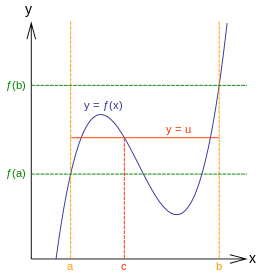
\includegraphics{resources/Intermediatevaluetheorem.png}
\end{center}
}%介值定理结尾

\subsection{二项式定理}{
  $(x + y)^n = x^n + \mathCombination{n - 1}{n}(x^{n-1} y) + \mathCombination{n - 2}{n}(x^{n-2} y^2) + \dots + y^n$

  \subsubsection{二项式系数与帕斯卡三角形(杨辉三角)}{

    二项式系数是二项式定理中各项的系数.一般而言,二项式系数由两个非负整数$n$和$k$作为参数来决定,写作$\begin{pmatrix}
        n \\
        k
      \end{pmatrix}$,定义为$(1 + x)^n$的多项式展开式中$x^k$项的系数,因此一定是非负整数.

    如果将二项式系数$\binom{n}{0},\binom{n}{1},\dots,\binom{n}{n}$写成一行,再依照$n = 0,1,2,3,...$顺序由上往下排列,则构成帕斯卡三角形(杨辉三角) :
    \begin{center}
      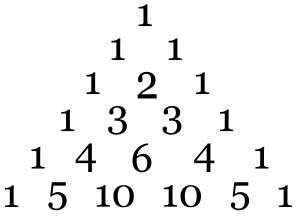
\includegraphics[scale=0.5]{resources/Pascal's_triangle_5.svg.png}
    \end{center}

    事实上,二项式系数就是排列组合中的组合 : ($\mathCombination{m}{n} \Longleftrightarrow \binom{m}{n}$)

    此外也有不同的表达方式 : $C(n,k),~_nC_k,~^nC_k,C^k_n,C^n_k\dots$

    %# TODO 看看Wiki : https://zh.wikipedia.org/wiki/%E4%BA%8C%E9%A0%85%E5%BC%8F%E4%BF%82%E6%95%B8
  }%二项式系数结尾

}%二项式定理结尾

\subsection{排列组合}{

  排列:$\mathPermutation{m}{n} = \cfrac{m!}{(m-n)!}$

  组合:$\mathCombination{m}{n} = \cfrac{\mathPermutation{m}{n}}{m!} = \cfrac{n!}{m!(n-m)!}$
}%排列组合结尾

\subsection{立方差公式}{
  \begin{itemize}
    \item $a^3 + b^3 = (a + b)(a^2 - ab + b^2)$
    \item $a^3 - b^3 = (a - b)(a^2 + ab + b^3)$
  \end{itemize}
}%立方差公式结尾

\subsection{等幂求和公式}{

}%等幂求和公式

\subsection{圆幂定理}{
  给定一个圆$r$及一点p,由p引出两条割线,分别于$r$相交于$A,B$及$C,D$,则有$PA \cdot PB = PC \cdot PD$

  事实上此定理包含三条定理 :

  \subsubsection{割线定理}{
    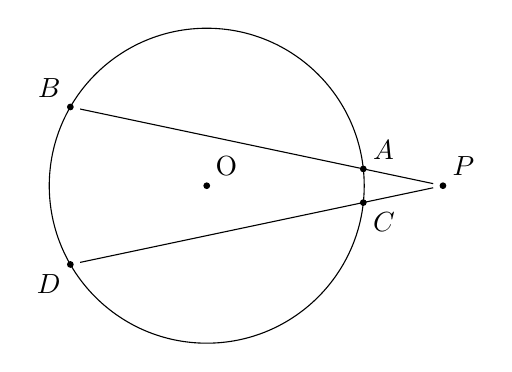
\begin{tikzpicture}
      \node (o) at (0.25,0.25){O};
      \draw [fill = black] (0,0) circle (1pt);
      \path[name path= c,draw] (0,0) circle (2);
      \node (B) at (-{sqrt(3)},1) {};
      \node (D) at (-{sqrt(3)},-1) {};
      \node (P) at (3,0){};
      \draw [fill = black] (P) circle (1pt);
      \draw [fill = black] (B) circle (1pt);
      \draw [fill = black] (D) circle (1pt);

      \path[name path = l1,draw] (B) node[above left]{$B$} -- (P) node [above right]{$P$};
      \path[name path = l2,draw] (D) node[below left]{$D$} -- (P);

      \node[name intersections = {of = c and l1,by=x}] (A) at (x){};
      \node[name intersections = {of = c and l2,by=x}] (C) at (x){};

      \draw [fill = black] (A) circle (1pt) node[above right]{$A$};
      \draw [fill = black] (C) circle (1pt) node[below right]{$C$};
    \end{tikzpicture}
    $PA \cdot PB = PC \cdot PD$
  }%割线定理结尾

  \subsubsection{交弦定理}{
    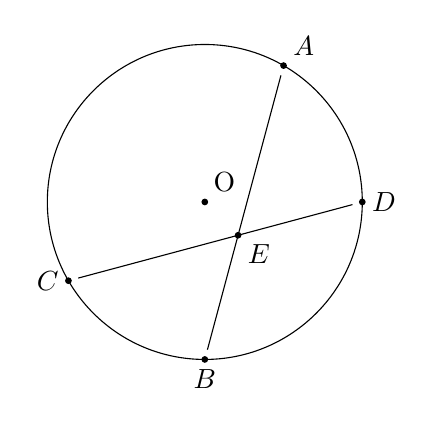
\begin{tikzpicture}
      \node (o) at (0.25,0.25){O};
      \draw [fill = black] (0,0) circle (1pt);
      \path[draw] (0,0) circle (2);
      \node (A) at (1,{sqrt(3)}){};
      \node (C) at ({-sqrt(3)},-1){};
      \node (D) at (2,0){};
      \node (B) at (0,-2){};
      \path[draw,name path = l1] (A) -- (B);
      \path[draw,name path = l2] (D) -- (C);
      \node[name intersections = {of = l1 and l2,by = x}] (E) at (x){};

      \draw [fill = black] (A) circle (1pt) node[above right]{$A$};
      \draw [fill = black] (B) circle (1pt) node[below]{$B$};
      \draw [fill = black] (C) circle (1pt) node[left]{$C$};
      \draw [fill = black] (D) circle (1pt) node[right]{$D$};
      \draw [fill = black] (E) circle (1pt) node[below right]{$E$};
    \end{tikzpicture}
    $EA \cdot EB = EC \cdot ED$
  }%交弦定理结尾

  \subsubsection{切割线定理}{
    \begin{tikzpicture}
      \node (o) at (0.25,0.25){O};
      \draw [fill = black] (0,0) circle (1pt);
      \path[name path= c,draw] (0,0) circle (2);

      \node (T) at (0,2){};
      \node (B) at ({-sqrt(3)},-1){};
      \node (P) at (5,2){};

      \draw (T) -- (P);
      \path[draw,name path = l1] (B) -- (P);

      \node[name intersections = {of = c and l1,by = x}] (A) at (x){};

      \draw [fill = black] (A) circle (1pt) node[above right]{$A$};
      \draw [fill = black] (B) circle (1pt) node[above left]{$B$};
      \draw [fill = black] (T) circle (1pt) node[above]{$T$};
      \draw [fill = black] (P) circle (1pt) node[right]{$P$};
    \end{tikzpicture}
    $PT^2 = PA \cdot PB$
  }%切割线定理结尾

}%圆幂定理结尾

\subsection{圆周角定理}{
  一条弧所对的圆周角$\alpha$等于所对圆心角的一半.

  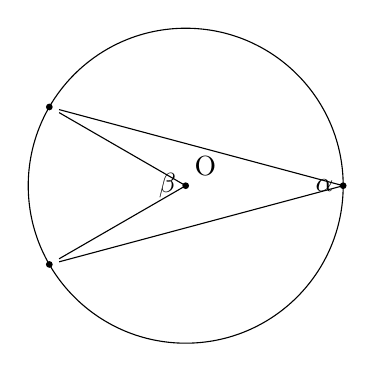
\begin{tikzpicture}
    \node (o) at (0.25,0.25){O};
    \draw [fill = black] (0,0) circle (1pt);
    \path[name path= c,draw] (0,0) circle (2);
    \node (P1) at (-{sqrt(3)},1) {};
    \node (P2) at (-{sqrt(3)},-1) {};

    \draw (P1) -- (2,0) node[left]{$\alpha$} -- (P2);
    \draw (P1) -- (0,0) node[left]{$\beta$} -- (P2);

    \tikzPlaceDot{(P1)};
    \tikzPlaceDot{(P2)};
    \tikzPlaceDot{(2,0)};
  \end{tikzpicture}

}%圆周角定理结尾

\subsection{韦达定理}{
\subsubsection{韦达定理的普遍情况}{
设$P(x) = a_nx^n + a_{n-1}x^{n-1} + \dotsm + a_1x + a_0$是一个一元n次实(或复)系数多项式,首项系数$a_n \neq 0$,令P的n个根为$x_1,x_2,\dots,x_n$,则根$\{x_i\}$和系数$\{a_j\}$之间满足关系式 :

$$
  \begin{cases}
    x_1 + x_2 + \dotsm + x_{n-1} + x_n = -\cfrac{a_{n-1}}{a_n}                                                           \\
    (x_1x_2 + x_1x_3 + \dotsm + x_1x_n) + (x_2x_3 + x_2x_4 + \dotsm + x_2x_n) + \dotsm + x_{n-1}x = \cfrac{a_{n-2}}{a_n} \\
    \vdots                                                                                                               \\                                                                                                               \\
    x_1x_2 \dotsm x_n = (-1)^n\cfrac{a_n}{a_n}
  \end{cases}
$$

等价的说,对任何$k = 1,2,\dots,n$,系数比$\cfrac{a_{n-k}}{a_n}$是所有任取k个根的乘积的和的$(-1)^k$倍,即 :

$\sum\limits_{1 \leq i_1 < i_2 < \dotsm < i_k \leq n}x_{i_{1}}x_{i_{2}} \dotsm x_{i_{k}} = (-1)^k\cfrac{a_{n-k}}{a_n}$

其中$i_1 < i_2 < \dotsm < i_k$是要让所有根的组合都恰好出现一次.

(等号的左边被称作是初等对称多项式)
}%韦达定理的普遍情况结尾

\subsubsection{n = 2的情况(二次)}{
  设$x_1,x_2$是一元二次多项式$ax^2 + bx + c$的两根,则由$ax^2 +bx + c = a(x - x_1)(x - x_2) = ax^2 - a(x_1 + x_2)x + ax_1x_2$有 :

  $x_1 + x_2 = -\cfrac{b}{a},\qquad x_1x_2 = \cfrac{c}{a}$

  在这个情况下,韦达定理的逆定理同样成立 : 给定一个一元二次多项式$ax^2 + bx + c$,如果有两个数$x_1,x_2$,满足$x_1 + x_2 = -\cfrac{b}{a}$和$x_1x_2 = \cfrac{c}{a}$,则$x_1,x_2$就是多项式$ax^2 + bx + c$的两根.
}%n = 2的情况(二次)结尾

\subsubsection{n = 3的情况(三次)}{
  设$x_1,x_2,x_3$是一元三次多项式$ax^3 + bx^2 + cx + d$的三根,则

  $x_1 + x_2 + x_3 = -\cfrac{b}{a}, x_1x_2 + x_1x_3 + x_2x_3 = \cfrac{c}{a},x_1x_2x_3 = -\cfrac{d}{a}$
}%n = 3的情况(三次)结尾

}%韦达定理结尾

\subsection{极坐标}{
极坐标是不同于笛卡尔坐标系(直角坐标系)的另一种函数图像平面.

极坐标不同于笛卡尔坐标系,他没有x和y轴,而是用基准轴和角度表示一个点.

\subsubsection{极坐标系下的面积}{
  \begin{center}
    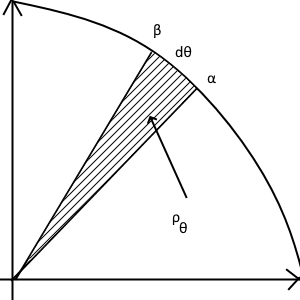
\includegraphics{resources/polar_coordness.png}
  \end{center}

  公式为$\cfrac{1}{2}\definiteIntegral{\beta}{\alpha}(p(\theta))^2d\theta$

  p是形成曲线的函数.
  }%极坐标下的面积结尾

  \subsubsection{转换公式}{
    从直角坐标系到极坐标有一套转换公式.

    $$
      \begin{cases}
        x = \rho\cos\theta \\
        y = \rho\sin\theta
      \end{cases}
    $$
  }%转换公式结尾

  \subsubsection{极坐标表示线}{
    \begin{center}
      \begin{tikzpicture}
        \draw (0,0) -- (0,5);
        \draw[->] (0,0) -- (5,0);
        \node (p1) at (1,4){(a,b)};
        \node (p2) at (3,1){(c,d)};
        \draw (p1) -- (p2);
      \end{tikzpicture}
    \end{center}

    由转换公式,可以将直线在直角坐标系下的解析式$y = kx + b$转换为在极坐标下的解析式 :
    $$
      \rho\sin\theta = k\rho\sin\theta + b
    $$
    再变形得到 :
    $$
      \rho = \cfrac{b}{\sin\theta - k\cos\theta}
    $$
  }%极坐标表示线结尾

  \subsubsection{极坐标表示面}{
    所谓"线动成面",想要用极坐标表示面,只需要加上$\rho$的取值条件就行(即 : $a \leq \rho \leq b$,此处的$a,b$也可以是关于其他变量的公式).
  }%极坐标表示面结尾

  \subsubsection{柱面坐标}{
    柱面坐标是一种将极坐标扩展到三维的方法,其实就是加了个z轴.因此转换公式为 :

    $$
      \begin{cases}
        x = \rho\cos\theta \\
        y = \rho\sin\theta \\
        z = z
      \end{cases}
    $$
  }%柱面坐标结尾

  \subsubsection{球面坐标}{
    球面坐标又是不同与柱面坐标的另一种形式,他引入了另一个表示角度的变量$\varphi$

    球面坐标由三个变量组成,如果将某一个点用向量$\vec{v}$表示,那么三个变量分别是 :
    \begin{itemize}
      \item $r$ : 表示$\vec{v}$的长度,可以理解成极坐标的$\rho$.取值范围为:$\left[0,+\infty\right)$
      \item $\theta$ : 用过原点以$z$轴作为法向量的平面作为极坐标的平面,$\vec{v}$投影到此平面上时$\theta$就是该投影在极坐标中的角度单位.取值范围为$\mediumBigCase{0,2\pi}$
      \item $\varphi$ : 以原点为顶点,$z$轴为旋转轴,$\vec{v}$作为母线的圆锥面的半顶角.也就是$\vec{v}$与$z$轴的夹角.取值范围为:$\mediumBigCase{0,\pi}$
    \end{itemize}

    从直角坐标系到球面坐标系的转换公式为 :
    $$
      \begin{cases}
        x = r\sin\varphi\cos\theta \\
        y = r\sin\varphi\sin\theta \\
        z = r\cos\varphi
      \end{cases}
    $$
  }%球面坐标结尾

}%极坐标结尾

\subsection{不等式}{

\subsubsection{基本不等式}{
  $\cfrac{a + b}{2} \geq \sqrt{ab}$

  注:当且仅当$a = b$时取等号

  其中$\cfrac{a+b}{2}$称为$a,b$的算数平均数,$\sqrt{ab}$称为$a,b$的几何平均数.

  将其变形,可得:
  \begin{enumerate}
    \item $a + b \geq 2\sqrt{ab}$(当且仅当$a = b$时取等号)
    \item $\cfrac{b}{a} + \cfrac{a}{b} \geq 2$($a,b$同号)
    \item $ab \leq (\cfrac{a + b}{2})^2$($a,b\in\mathRealNumberCollection$)
    \item $(\cfrac{a + b}{2})^2 \leq \cfrac{a^2 + b^2}{2}$($a,b\in\mathRealNumberCollection$)
  \end{enumerate}
}%基本不等式结尾


\subsubsection{柯西不等式}{
  柯西不等式有很多种形式:
  \begin{itemize}
    \item {
          二维形式:

          由$(a^2 + b^2)(c^2 + d^2)\geq(ac + bd)^2$变形:$ac + bd \leq \sqrt{(a^2 + b^2)(c^2 + d^2)}$

          当且仅当$ab = cd$(即$\cfrac{a}{c} = \cfrac{b}{d}$)时.

          一般形式为$\upDownSum{n}{i = 1}a_i^2\upDownSum{n}{i = 1}b_i^2\geq\bigCase{\upDownSum{n}{i = 1}a_ib_i)}^2$

          当$\cfrac{a_1}{b_1} = \cfrac{a_2}{b_2} = \dots = \cfrac{a_n}{b_n}$或$a_i,b_i,i = 1,2,3,\dots,n$中至少有一方全为$0$时等号成立.

          一般形式推广:$(x_1 + y_1 + \dots)(x_2 + y_2 + \dots)\dots(x_n + y_n + \dots) \geq \left[\bigCase{\upDownProd{n}{i = 1}x_i}^{\cfrac{1}{n}} + \bigCase{\upDownProd{n}{i = 1}y_i}^{\cfrac{1}{n}} + \dots\right]^n$

          此推广形式又称卡尔松不等式,其表述是:在m×n矩阵中,各列元素之和的几何平均不小于各行元素的几何平均之和.二维形式是卡尔松不等式n=2时的特殊情况.
          }
    \item {
          向量形式:

          对于内积空间中的向量$\vec{x}$和$\vec{y}$,有

          $|\innerProduct{\vec{x}}{\vec{y}}^2| \leq \innerProduct{\vec{x}}{\vec{x}} \times \innerProduct{\vec{y}}{\vec{y}}$

          其中$\innerProduct{\cdot}{\cdot}$表示内积.等价地,将两边开方,等式右边即可以写为两向量范数乘积的形式.

          $|\innerProduct{\vec{x}}{\vec{y}}| \leq ||\vec{x}||\cdot||\vec{y}||$.

          另外,当且仅当$x$和$y$线性相关时,等号成立(仅两个向量而言,线性相关等同于平行).

          若$x_1,\dotsm,x_n \in \mathConstant$和$y_1,\dotsm,y_n \in mathConstant$有虚部,内积即为标注内积.如果用上划线标记共轭复数,这个不等式可以更明确的表述为:

          $|\vec{x_1}\bar{\vec{y_1}} + \dotsm + \vec{x_n}\bar{\vec{y_n}}|^2\leq (|\vec{x_1}|^2 + \dotsm + |\vec{x_n}|^2)(|\vec{y_1}|^2 + \dotsm + |\vec{y_n}|^2)$.
          }
    \item {
          三角形式:

          在三角形$ABC$中,这个式子可以写作:$||\vec{AB}|| + ||\vec{BC}|| \geq ||\vec{AC}||$

          也就是说:$\sqrt{a^2 + b^2} + \sqrt{c^2 + d^2} \geq \sqrt{(a - c)^2 + (b - d)^2}$

          等号成立的条件为:$ad = bc,且ac + bc \geq 0$(即$\cfrac{a}{c} = \cfrac{b}{d}$).
          }
    \item {
          积分形式:

          $\bigCase{\int\defFunction{x}g(x)dx}^2 \leq \int\fint^2(x)dx \int g^2(x)dx$
          }
    \item {
          一般形式:

          设$V$是一线性空间,定义内积,记作$\innerProduct{\alpha}{\beta}$,则:

          $|\innerProduct{\alpha}{\beta}| \leq |\alpha||\beta|$.

          其中$\alpha,\beta$为$V$中的向量.
          }
  \end{itemize}
}%柯西不等式结尾

\subsubsection{均值不等式}{
平均数不等式,或称平均值不等式、均值不等式,是数学上的一组不等式,也是基本不等式的推广.它是说:

如果$x_{1},x_{2},\dotsm,x_{n}$是正数,则:

$\mathbf{H}_n \leq \mathbf{G}_n \leq \mathbf{A}_n \leq \mathbf{Q}_n$

其中:

$\mathbf{H}_n = \cfrac{n}{\upDownSum{n}{i = 1}\cfrac{1}{x_i}} = \cfrac{n}{\cfrac{1}{x_1} + \cfrac{1}{x_2} + \dotsm + \cfrac{1}{x_n}}$

$\mathbf{G}_n = \sqrt[n]{\upDownProd{n}{i = 1}x_i} = \sqrt[n]{x_1x_2\dotsm x_n}$

$\mathbf{A}_n = \cfrac{\upDownSum{n}{i = 1}x_i}{n} = \cfrac{x_1 + x_2 + x_n}{n}$

$\mathbf{Q}_n = \sqrt{\cfrac{\upDownSum{n}{i = 1}x^2_i}{n}} = \sqrt{\cfrac{x^2_1 + x^2_2 + \dotsm + x^2_n}{n}}$

当且仅当$x_1 = x_2 = \dotsm = x_n$,等号成立.

当$n = 2$时:

$\cfrac{2}{\cfrac{1}{x_1} + \cfrac{1}{x_2}} = \cfrac{2x_1x_2}{x_1 + x_2}\leq\sqrt{x_1x_2}\leq\cfrac{x_1 + x_2}{2}\leq\sqrt{\cfrac{x_1^2 + x_2^2}{2}}$

即对这些正数:调和平均数$\leq$几何平均数$\leq$算数平均数$\leq$平方平均数(方均根)

可简记为:“{\bfseries 算几调方}”
}%二元均值不等式结尾  

\subsubsection{算术-几何均值不等式}{
  算术-几何平均值不等式,简称算几不等式,是一个常见而基本的不等式,表现算术平均数和几何平均数之间恒定的不等关系.设$x_1,x_2,\dots,x_n$为$n$个正实数,他们的算数平均数是$\mathbf{A}_n = \cfrac{x_1 + x_2 + \dotsm + x_n}{n}$,他们的几何平均数是$\mathbf{G}_n = \sqrt[n]{x_1\cdot x_2 \dotsm x_n}$.算术-几何平均值不等式表明,对任意的正实数$x_1,\dotsm,x_n$,总有:

  \begin{center}
    $\mathbf{A}_n\geq\mathbf{G}_n$
  \end{center}

  等号当且仅当$x_1 = x_2 = \dotsm = x_n$时成立.

}%算术-几何均值不等式结尾

\subsubsection{常用不等式}{
  \begin{itemize}
    \item $a^2 + b^2 \geq \cfrac{1}{2}(a + b)^2$
    \item $a^2 + b^2 \geq 2ab$
    \item $ab \leq \cfrac{a^2 + b^2}{2}$
    \item $ab \leq (\cfrac{a + b}{2})^2$
    \item $a + b \geq 2\sqrt{ab}$
    \item $a + b \leq \sqrt{2(a^2 + b^2)}$
  \end{itemize}
}%常用不等式结尾

}%不等式结尾

\subsection{可微,可导,连续的关系}{

  \subsubsection{一元情况下的关系}{
    \begin{itemize}
      \item 可微是可导的充要条件,即:可微$\Leftrightarrow$可导
      \item 可微和可导都是连续的充分条件,即:可微$\rightarrow$连续、可导$\rightarrow$连续
    \end{itemize}

    \begin{center}
      \begin{tikzpicture}
        \node(a) at (0,1.5) {可微};
        \node(b) at (3,1.5) {可导};
        \node(c) at (1.5,0) {连续};
        \draw[<->] (a) -- (b);
        \draw[->] (a) -- (c);
        \draw[->] (b) -- (c);
      \end{tikzpicture}
    \end{center}
  }%一元情况下的关系结尾

  \subsubsection{多元情况下的关系}{
    \begin{itemize}
      \item 可微(全微分)是可导和连续的充分条件,即:可微$\Rightarrow$可导、可微$\Rightarrow$连续.
      \item 可导$\nRightarrow$连续.
    \end{itemize}

    \begin{center}
      一元 :
      \begin{tikzpicture}
        \node(a) at (0,1.5) {可微};
        \node(b) at (3,1.5) {可导};
        \node(c) at (1.5,0) {连续};
        \draw[->] (a) -- (b);
        \draw[->] (a) -- (c);
      \end{tikzpicture}
    \end{center}
  }%多元情况下的关系结尾

}%可微,可导,连续的关系结尾

\subsection{映射与函数}{

  \subsubsection{映射}{
    映射指的是集合之间的一种对应关系.

    定义 : $X,Y$是两集合,按照某个规则$f$,对于任一的$x \in X$,有唯一的$y \in Y$与之对应,则称$f$是$X$到$Y$的一个映射.

    记为 : $f: X \to Y$,即 : $x \mapsto y = \defFunction{x}$

    称呼 :

    \begin{itemize}
      \item $y$ : 在映射$f$下,x的像.
      \item $x$ : 在映射$f$下,y的\textcolor{red}{一个}逆像.
      \item $X$ : $f$的定义域,记为$X = D_f$.
      \item $Y$ : $f$的值域,记为$R_f \subset Y$,具体的来说,$R_f = \set{y | y \in Y \land \exists x(y = f(x) \land x \in X)}$
    \end{itemize}

    举例 : 设$X$是平面上三角形的全体,$Y$是平面上圆的全体,构造一个映射$f$,表示(y 是 x 的外接圆),记为 : $$
      f : \underset{x \mapsto y}{X \to Y}
    $$
  }%映射结尾

  \subsubsection{映射的基本要素}{
    \begin{itemize}
      \item $X = D_f$,定义域.
      \item $Y$,限制值域的范围.
      \item $f$,需要保证像的唯一性.
    \end{itemize}

    这说明了两点 : \begin{enumerate}
      \item {
            映射的像是唯一的,举例 :

            设$X = \mathRealNumberCollection^+ = \set{x | x \in R \land x > 0}$,假设存在映射$f : \underset{x \mapsto y}{X \to Y}(y^2 = x)$,此时$Y = \mathRealNumberCollection$,那么假设$x = 4,y = \pm 2$.这个映射就无法保证像的唯一性.换句话说,这个$f$并不是个映射.

            但是可以稍作改造:对$Y = \mathRealNumberCollection$做限制,令$Y = R^-$,此时 : $$
              \mapsToWithSubText{f}{X \to Y}{x \mapsto y}(y^2 = x)
            $$
            就构成了一个映射
            }
      \item {
            映射不要求逆向唯一.
            }
    \end{enumerate}
  }%映射的基本要素结尾

  \subsubsection{映射的分类}{
    \begin{itemize}
      \item {
            单射 :

            $f$是$X$到$Y$的一个映射,若逆像也具有唯一性,则称$f$是单射(injection)

            逻辑命题表述 : $x_1 \neq x_2 \Rightarrow y_1 \neq y_2(y_1 = \defFunction{x_1},y_2 = \defFunction{x_2})$

            注 : 单射的值域不一定完全等于$Y$,也可能包含于$Y$,即$R_f \subseteq Y$
            }
      \item {
            满射 : 如果映射的值域完全等于$Y$,即$R_f = Y$,则称为满射(surjection).

            注 : 满射不一定是单射
            }
      \item {
            双射 : 如果$f$又是单射,又是满射,则称$f$为双射(bijection)

            双射又称为一一对应.
            }
    \end{itemize}
  }%映射的分类结尾

  \subsubsection{逆映射}{
    如果$f : X \to Y$是一个单射,即对任意的$y \in R_f$,有唯一的逆像$x \in X$与$y$对应.

    如果$\mapsToWithSubText{g}{R_f \to X}{y \mapsto x}$是满射($\defFunction{x} = y$)

    那么$g$就称为$f$的逆映射,又记为$f\inverse$

    举例 : $\mapsToWithSubText{y = \sin x}{\mediumBigCase{-\frac{\pi}{2},\frac{\pi}{2}} \to \mediumBigCase{-1,1}}{x \mapsto y = \sin x}$,他的逆映射为 : $$
      \mapsToWithSubText{x = \arcsin y}{\mediumBigCase{-1,1} \to \mediumBigCase{-\frac{\pi}{2},\frac{\pi}{2}}}{y \mapsto x}(\sin x = y)
    $$
  }%逆映射结尾

  \subsubsection{复合映射}{
    $$
      \mapsToWithSubText{g}{X \to U_1}{x \mapsto u = g(x)}
    $$
    $$
      \mapsToWithSubText{f}{U_2 \to Y}{u \mapsto y = f(u)}
    $$

    这两个映射若是要复合在一起,那么就得满足 : $R_g \subset U_2 = D_f$.即 : $g$的值域在$f$的定义域中,才能构造出复合映射.

    称为$f$与$g$的复合映射.

    例 : 设$X = Y = U_1 = U_2 = \mathRealNumberCollection$ :
    $$
      \mapsToWithSubText{g}{x \to U_1}{x \mapsto u = \sin x}
    $$
    $$
      \mapsToWithSubText{f}{U_2 \to Y}{u \mapsto y = \frac{u}{1 + u^2}}
    $$
    由于$R_g = \mediumBigCase{-1,1} \subset D_f$,所以 : $$
      \mapsToWithSubText{f \cdot g}{X \to Y}{x \mapsto y = \frac{\sin x}{1 + \sin x}}
    $$
  }%复合映射结尾

}%映射与函数结尾

\subsection{零散的定义}{
  \begin{enumerate}
    \item 有界:$\exists\epsilon,f(x) < \epsilon\quad(-\infty < x < \infty )$
    \item 什么时候函数能复合 : 内层值域$\in$外层定义域
  \end{enumerate}
}%零散的定义结尾

\subsection{零散的思想}{
  \begin{enumerate}
    \item 正变换是数学的重要工具,三角变换是只变其形不变其质的.三角变换常常先寻找式子所包含的各个角之间的联系,并以此为依据选择可以联系它们的适当公式,通过换元法把三角恒等变换问题转化为代数恒等变换问题.
  \end{enumerate}
}%零散的思想结尾

}%基本概念结尾
  %*三角函数
  %  \section{三角函数}{
三角函数一般由单位圆引出,如下:

\begin{center}
  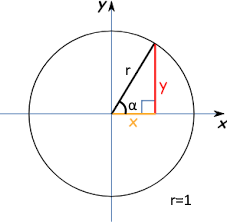
\includegraphics{resources/UnitCircle.png}
\end{center}

\subsection{正三角函数}{
  \begin{tabular}{|c|c|c|c|}
    \hline
    名字           & 定义           & 定义域                                                                                       & 值域                                \\
    \hline
    $\sin{\alpha}$ & $\cfrac{y}{r}$ & $\mathRealNumberCollection$                                                                  & $\mediumBigCase{-1,1}$              \\
    \hline
    $\cos{\alpha}$ & $\cfrac{x}{r}$ & $\mathRealNumberCollection$                                                                  & $\mediumBigCase{-1,1}$              \\
    \hline
    $\tan{\alpha}$ & $\cfrac{y}{x}$ & $\mathRealNumberCollection(\alpha \neq \cfrac{\pi}{2} + k\pi(k \in \mathIntegerCollection))$ & $\mathRealNumberCollection$         \\
    \hline
    $\cot{\alpha}$ & $\cfrac{x}{y}$ & $\mathRealNumberCollection(\alpha \neq k\pi(k \in \mathIntegerCollection))$                  & $\mathRealNumberCollection$         \\
    \hline
    $\sec{\alpha}$ & $\cfrac{r}{x}$ & $\mathRealNumberCollection(\alpha \neq k\pi + \cfrac{\pi}{2}(k \in \mathIntegerCollection))$ & $\absoluteValue{\sec\alpha} \geq 1$ \\
    \hline
    $\csc{\alpha}$ & $\cfrac{r}{y}$ & $\mathRealNumberCollection(\alpha \neq k\pi + \cfrac{\pi}{2}(k \in \mathIntegerCollection))$ & $\absoluteValue{\csc\alpha} \geq 1$ \\
    \hline
  \end{tabular}
}%正三角函数结尾

\subsection{反三角函数}{
  \begin{tabular}{|c|c|c|c|}
    \hline
    名字        & 定义         & 定义域                                                     & 值域                                                                      \\
    \hline
    $\arcsin x$ & $x = \sin y$ & $\mediumBigCase{-1,1}$                                     & $\mediumBigCase{-\cfrac{\pi}{2},\cfrac{\pi}{2}}$                          \\
    \hline
    $\arccos x$ & $x = \sin y$ & $\mediumBigCase{-1,1}$                                     & $\mediumBigCase{0,\pi}$                                                   \\
    \hline
    $\arctan x$ & $x = \tan y$ & $\mathRealNumberCollection$                                & $\mediumBigCase{-\cfrac{\pi}{2},\cfrac{\pi}{2}}$                          \\
    \hline
    $\arccot x$ & $x = \cot y$ & $\mathRealNumberCollection$                                & $\mediumBigCase{0,\pi}$                                                   \\
    \hline
    $\arcsec x$ & $x = \sec y$ & $\left(-\infty,-1\right] \unionSet \left[1,+\infty\right)$ & $\left[0,\cfrac{\pi}{2}\right) \unionSet \left(\cfrac{\pi}{2},\pi\right]$ \\
    \hline
    $\arccsc x$ & $x = \csc y$ & $\left(-\infty,-1\right] \unionSet \left[1,+\infty\right)$ & $\left[-\cfrac{\pi}{2},0\right) \unionSet \left(0,\cfrac{\pi}{2}\right]$  \\
    \hline
  \end{tabular}
}%反三角函数结尾

\subsection{和差化积}{
  $\sin{\alpha}+\sin{\beta} = 2\sin{\cfrac{\alpha + \beta}{2}}\cos{\cfrac{\alpha - \beta}{2}}$

  $\cos{\alpha}+\cos{\beta} = 2\cos{\cfrac{\alpha + \beta}{2}\cos{\cfrac{\alpha-\beta}{2}}}$

  $\cos{\alpha}-\cos{\beta} = -2\sin{\cfrac{\alpha + \beta}{2}}\cos{\cfrac{\alpha - \beta}{2}}$

  $\sin{\alpha}-\sin{\beta} = 2\sin{\cfrac{\alpha + \beta}{2}}\cos{\cfrac{\alpha - \beta}{2}}$

  $\tan\alpha - \tan\beta = \tan(\alpha - \beta) \cdot (1 + \tan\alpha\tan\beta)$
}%和差化积结尾

\subsection{积化和差}{
  $\cos(\alpha + \beta) = \cos{\alpha}\cos{\beta} - \sin{\alpha}\sin{\beta}$

  $\cos(\alpha - \beta) = \cos{\alpha}\cos{\beta} + \sin{\alpha}\sin{\beta}$

  $\sin(\alpha \pm \beta) = \sin{\alpha}\cos{\beta} \pm \cos{\alpha}\sin{\beta}$

  $\tan(\alpha + \beta) = \cfrac{\tan\alpha + \tan\beta}{1 - \tan\alpha\tan\beta}$

  $\tan(\alpha - \beta) = \cfrac{\tan\alpha - \tan\beta}{1 + \tan\alpha\tan\beta}$

  $\sin{\alpha}\cos{\beta} = \cfrac{1}{2}[\sin{(\alpha + \beta)} + \sin{(\alpha - \beta)}]$

  $\cos{\alpha}\cos{\beta} = \cfrac{1}{2}[\cos{(\alpha + \beta)} + \cos{(\alpha - \beta)}]$

  $\sin{\alpha}\sin{\beta} = -\cfrac{1}{2}[\cos{(\alpha + \beta)} - \cos{(\alpha - \beta)}]$
}%积化和差结尾

\subsection{诱导公式}{
  \indent 奇变偶不变,符号看象限.
  \subsubsection{第一组诱导公式}{
    $\sin{(2k\pi + \alpha)} = \sin{\alpha}$

    $\cos{(2k\pi + \alpha)} = \cos{\alpha}$

    $\tan(2k\pi + \alpha) = \tan\alpha$

    $\cot(2k\pi + \alpha) = \cot\alpha$
  }%第一组诱导公式结尾

  \subsubsection{第二组诱导公式}{
    $\sin(-\alpha) = -\sin\alpha$

    $\cos(-\alpha) = \cos\alpha$

    $\tan(-\alpha) = -\tan\alpha$

    $\cot(-\alpha) = -\cot\alpha$
  }%第二组诱导公式结尾

  \subsubsection{第三组诱导公式}{
    $\sin(\pi + \alpha) = -\sin\alpha$

    $\cos(\pi + \alpha) = -\cos\alpha$

    $\tan(\pi + \alpha) = \tan\alpha$

    $\cot(\pi + \alpha) = \cot\alpha$
  }%第三组诱导公式结尾

  \subsubsection{第四组诱导公式}{
    $\sin(\pi - \alpha) = \sin\alpha$

    $\cos(\pi - \alpha) = -\cos\alpha$

    $\tan(\pi - \alpha) = -\tan\alpha$

    $\cot(\pi - \alpha) = -\cot\alpha$
  }%第四组诱导公式结尾

  \subsubsection{第五组诱导公式}{
    $\sin(\cfrac{\pi}{2} - \alpha) = \cos\alpha$

    $\cos(\cfrac{\pi}{2} - \alpha) = \sin\alpha$

    $\tan(\cfrac{\pi}{2} - \alpha) = \cot\alpha$

    $\cot(\cfrac{\pi}{2} - \alpha) = \tan\alpha$
  }%第五组诱导公式结尾

  \subsubsection{第六组诱导公式}{
    $\sin(\cfrac{\pi}{2} + \alpha) = \cos\alpha$

    $\cos(\cfrac{\pi}{2} + \alpha) = -\sin\alpha$

    $\tan(\cfrac{\pi}{2} + \alpha) = -\cot\alpha$

    $\cot(\cfrac{\pi}{2} + \alpha) = -\tan\alpha$
  }%第六组诱导公式结尾

  \subsubsection{杂项}{
    $a\sin x + b\cos x = \sqrt{a^2 + b^2}\sin(x + \arctan\cfrac{b}{a}),(a > 0)$

    $a\sin x + b\cos x = \sqrt{a^2 + b^2}\cos x - \arctan\cfrac{a}{b}$

    $\cos\alpha = 2cos^2\cfrac{\alpha}{2} - 1 = 1-2\sin^2\cfrac{\alpha}{2}$
  }%杂项结尾

}%诱导公式结尾

\subsection{倍角公式}{

  \subsubsection{二倍角公式}{
    二倍角公式:由两角和公式推出

    $\sin2\alpha = 2\sin\alpha\cos\alpha$

    $\cos2\alpha = \cos^2\alpha - \sin^\alpha = 2\cos^2\alpha - 1 = 1 - 2\sin^2\alpha$

    $\tan2\alpha = \cfrac{2\tan\alpha}{1 - \tan^2\alpha}$
  }%二倍角公式结尾

  \subsubsection{半倍角公式}{
    半倍角公式:将二倍角公式中的角$2\alpha$看作整体$\beta$,经过变形推出:

    $\sin\cfrac{\alpha}{2} = \pm\sqrt{\cfrac{1 - \cos\alpha}{2}}$

    $\cos\cfrac{\alpha}{2} = \pm\sqrt{\cfrac{1 + \cos\alpha}{2}}$

    $\tan\cfrac{\alpha}{2} = \pm\sqrt{\cfrac{1-\cos\alpha}{1+\cos\alpha}} = \cfrac{\sin\alpha}{1+\cos\alpha} = \cfrac{1-\cos\alpha}{\sin\alpha}$

    $\cot\cfrac{\alpha}{2} = \cfrac{1+\cos\alpha}{\sin\alpha} = \cfrac{\sin\alpha}{1-\cos\alpha}$

    $\sec\cfrac{\alpha}{2} = \cfrac{\pm\sqrt{\cfrac{\sec\alpha - 1}{2\sec\alpha}}2\sec\alpha}{\sec\alpha + 1} = \cfrac{\pm\sqrt{\cfrac{4\sec^3\alpha + \sec^2\alpha}{2\cos\alpha}}}{\sec\alpha + 1}$

    $\csc\cfrac{\alpha}{2} = \cfrac{\pm\sqrt{\cfrac{\sec\alpha - 1}{2\sec\alpha}}2\sec\alpha}{\sec\alpha - 1} = \cfrac{\pm\sqrt{\cfrac{3\sec^3\alpha - \sec^2\alpha}{2\sec\alpha}}}{\sec\alpha - 1}$
  }%半倍角公式结尾

  \subsubsection{n倍角公式}{
    $\cos{n\theta} = \upDownSum{\cfrac{n}{2}}{i = 0}[(-1)^i\mathCombination{2i + 1}{n}\cos^{n - 2i}\theta\sin^{2i}\theta]$

    $\sin{n\theta} = \upDownSum{\cfrac{n}{2}}{i = 0}[(-1)^i\mathCombination{2i + 1}{n}\cos^{n - 2i - 1}\theta\sin^{2i+1}\theta]$
  }%n倍角公式结尾

  \subsubsection{万能替换公式}{
    万能替换公式:尝试将正常的三角函数用半角公式表示时经过变形推出:

    角$\alpha(\alpha \neq 2k\pi + \pi ,k \in \mathbf{z})$的所有三角比都可以用 $\tan\cfrac{\alpha}{2}$表示.这组公式叫做万能替换公式

    $\sin\alpha = \cfrac{2\tan\cfrac{\alpha}{2}}{1+\tan^2\cfrac{\alpha}{2}}$

    $\cos\alpha = \cfrac{1 - \tan^2\cfrac{\alpha}{2}}{1 + \tan^2\cfrac{\alpha}{2}}$

    $\tan\alpha \cfrac{2\tan\cfrac{\alpha}{2}}{1 - \tan^2\cfrac{\alpha}{2}}$
  }%万能替换公式结尾

  \subsubsection{降幂公式}{
    三角函数中的降幂公式可降低三角函数指数幂.多项式各项的先后按照某一个字母的指数逐渐减少的顺序排列,叫做这一字母的降幂.直接运用二倍角公式就是升幂,将公式$\cos 2 \alpha$变形后可得到降幂公式.

    $\sin^2\alpha = \cfrac{1 - \cos2\alpha}{2}$

    $\cos^2\alpha = \cfrac{1 + \cos2\alpha}{2}$

    $\tan^2\alpha = \cfrac{1 - \cos2\alpha}{1 + \cos2\alpha}$
  }%降幂公式

}%倍角公式结尾

\subsection{三角恒等式}{

  倒数关系 :
  \begin{itemize}
    \item $\sin\alpha \cdot \csc\alpha = 1$
    \item $\cos\alpha \cdot \sec\alpha = 1$
    \item $\tan\alpha \cdot \cot\alpha = 1$
  \end{itemize}

  商数关系 :
  \begin{itemize}
    \item $\tan\alpha = \cfrac{\sin\alpha}{\cos\alpha}$
    \item $\cot\alpha = \cfrac{\cos x}{\sin x}$
  \end{itemize}

  平方关系 :
  \begin{itemize}
    \item $\sin^2\alpha + \cos^2\alpha = 1$
    \item $1 + \tan^2\alpha = \sec^2\alpha$
    \item $1 + \cot^2\alpha = \csc^2\alpha$
  \end{itemize}

  余角关系 :
  \begin{itemize}
    \item $\arcsin\alpha + \arccos\alpha = \cfrac{\pi}{2}$
    \item $\arctan\alpha + \arccot\alpha = \cfrac{\pi}{2}$
    \item $\arcsec\alpha + \arccsc\alpha = \cfrac{\pi}{2}$
  \end{itemize}

  负数关系 :
  \begin{itemize}
    \item $\arcsin-\alpha = -\arcsin\alpha$
    \item $\arccos-\alpha = \pi - \arccos\alpha$
    \item $\arctan-\alpha = -\arctan\alpha$
    \item $\arccot-\alpha = \pi - \arccot\alpha$
    \item $\arcsec-\alpha = \pi - \arcsec\alpha$
    \item $\arccsc-\alpha = -\arccsc\alpha$
  \end{itemize}

}%三角恒等式结尾

三角形的边角、面积、和外接圆半径之间有着密切的联系

\subsection{解斜三角形}{
设三角形$\triangle ABC$,角A、B、C的对边为abc,以A为原点$O$建系,总有以下公式:

$\mathbf{S}\triangle_{ABC} = \cfrac{1}{2}AB \cdot CD = \cfrac{1}{2}cb\sin A$,即$\mathbf{S}\triangle_{ABC} = \cfrac{1}{2}bc\sin A$

同理得:$\mathbf{S}\triangle_{ABC} = \cfrac{1}{2}\sin B, \mathbf{S}\triangle_{ABC} = \cfrac{1}{2}ab\sin C$.

这就是说,三角形的面积等于任意两边与他们夹角正弦值的一半.

\subsubsection{正弦定理}
将$\cfrac{1}{2}bc\sin A = \cfrac{1}{2}ac\sin B = \cfrac{1}{2}ab\sin C$三个公式同除$\cfrac{1}{2}abc$,得:

$\cfrac{\sin A}{a} = \cfrac{\sin B}{b} = \cfrac{\sin C}{c}$, 也可表示为:$\cfrac{a}{\sin A} = \cfrac{b}{\sin B} = \cfrac{c}{\sin C}$

此式表明:在三角形中,各{\bfseries边}与它所对{\bfseries角的正弦}的比相等

当$\angle C = 90\degree$时,由正弦定理可得:$\cfrac{\sin A}{a} = \cfrac{\sin B}{b} = \cfrac{1}{c}$,即$a = c\sin A,B = C\sin B$

并且,做三角形外接圆:

\begin{center}
  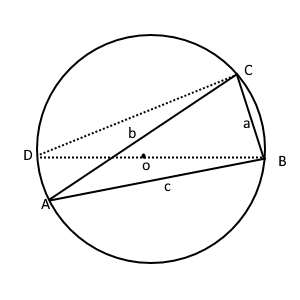
\includegraphics[scale=0.5]{resources/insideTriangleAndCircleOutSide.png}
\end{center}

由圆周角定理可知$\angle D = \angle A,BD = 2R,bc = a$.于是$a = BC = BD\sin A = 2R\sin A$,即:

$\cfrac{a}{\sin A} = 2R$

由正弦定理,可得:$\cfrac{a}{\sin A} = \cfrac{b}{\sin B} = \cfrac{c}{\sin C}$

所以,$a = 2R\sin A,b = 2R\sin B,c = 2R\sin C$

变形也可得到:

$\sin C = \cfrac{c}{2R},\sin B = \cfrac{b}{2R},\sin A = \cfrac{a}{2R}$

以及:

$a^2\sin2B + b^2\sin2A = 2ab\sin C$
}%解斜三角形结尾

\subsubsection{余弦定理}{
  由两点间距离公式,得$a = |BC| = \sqrt{(b\cos A - c)^2 + (b\sin A - 0)^2}$

  两边平方并化简得:

  $a^2 = b^2 - 2b\cos A + c^2$

  $b^2 = a^2 + c^2 - 2ac\cos B$

  $c^2 = a^2 + b^2 - 2ab\cos C$

  也可变形化为:

  $\cos A = \cfrac{b^2 + c^2 - a^2}{2bc}$

  $\cos B = \cfrac{a^2 + c^2 - b^2}{2ac}$

  $\cos C = \cfrac{b^2 + a^2 - c^2}{2ab}$
}%余弦定理结尾
\\

\indent这些关系在直角三角形中也成立.

}%三角函数结尾
  %*解析几何
  % \chapter{解析几何}{
  不容小觑且难以理解的部分,加油.

  \section{关于向量}{
    在空间解析几何部分不会引入过多有关线性代数的知识(比如向量空间).定理与定义将会互相交织.

    注:本章中的向量默认为三维向量.

    \subsection{关于向量的基本概念}{
      有以下概念:
      \begin{itemize}
        \item 数乘:$\lambda \vec{\alpha}$,即$\lambda$倍长度的$\vec{\alpha}$,当$\lambda > 0$时,方向与原向量相同.当$\lambda < 0$时,方向相反.数乘前后向量的起点一致.
        \item 取模:$|\lambda\vec{\alpha}| = |\lambda||\vec{\alpha}|$,前一个“$||$”为绝对值,后一个“$||$”为取模.最后得出的结果为$|\lambda\vec{\alpha}|$的长度.
        \item 单位化:$|\cfrac{\vec{\alpha}}{|\vec{\alpha}|}| = 1$,即将一个向量除以他的长度得到的是单位向量(长度为1的向量)
        \item 在三维标准正交坐标系中存在三个单位向量:$\vec{i},\vec{j},\vec{k}$.他们互相垂直,长度为1.坐标系中任意一点$(x,y,z)$都可以表示为一个向量$\vec{r},\vec{r} = x\vec{i} + y\vec{j} + z\vec{k}$.
        \item 设$\vec{a} = (ax,ay,az),\vec{b} = (bx,by,bz)$.则:$\vec{a} \pm \vec{b} = (ax \pm bx,ay \pm by,az \pm bz)$、$\lambda\vec{a} = (\lambda ax,\lambda ay,\lambda az)$.其中$ax,ay,az,bx,by,bz$称为分量.
        \item 平行:$\vec{b} = \lambda\vec{a},\cfrac{ax}{bx} = \cfrac{ay}{by} = \cfrac{az}{bz}$即:对应分量之比相同.
        \item 向量长度(取模)公式:$\vec{r} = (x,y,z),|\vec{r}| = \sqrt{x^2 + y^2 + z^2}$.注:对于任意维度的向量,取模都是各分量平方和开根号.
        \item 两点之间距离公式:$A:(x_1,y_1,z_1),B:(x_2,y_2,z_2),|\vec{AB}| = \sqrt{(x_1 - x_2)^2 + (y_1 -y_2)^2 + (z_1 - z_2)^2}$.注:在任意维度中,两点之间的距离公式都是对应分量作差的平方和开根号.
        \item {
              两向量夹角:(取锐角)设$\vec{a} = (a_1, a_2, a_3),\vec{b} = (b_1,b_2,b_3)$,设夹角为$\theta$,则:$\cos\theta = \cfrac{|a_1b_1 + a_2b_2 + a_3b_3|}{\sqrt{a_1^2 + a_2^2 + a_3^2}\sqrt{b_1^2 + b_2^2 + b_3^2}}$

              有以下几种情况:
              \begin{enumerate}
                \item 垂直:$a_1b_1 + a_2b_2 + a_3b_3 = 0$
                \item 平行:$\cfrac{a_1}{b_1} = \cfrac{a_2}{b_2} = \cfrac{a_3}{b_3}$
              \end{enumerate}

              求两直线夹角也同理.
              }
      \end{itemize}
    }%关于向量的基本概念结尾

    \subsection{方向角与方向余弦}{
      \begin{center}
        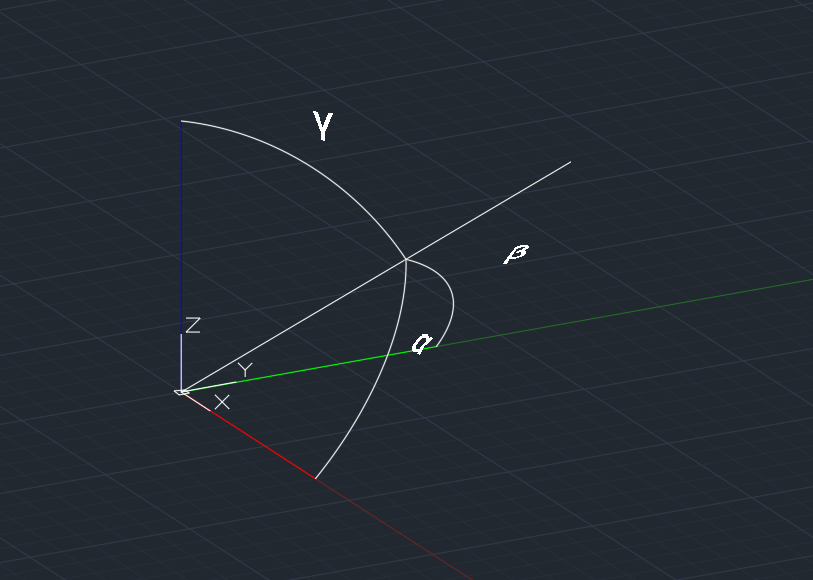
\includegraphics[scale = 0.5]{resources/directionAngle.png}
      \end{center}

      $\vec{OM} = \vec{r} = (x,y,z)$

      $\cos\alpha = \cfrac{x}{|\vec{OM}|} = \cfrac{x}{|\vec{r}|}$

      $\cos\beta = \cfrac{y}{|\vec{OM}|} = \cfrac{y}{|\vec{r}|}$

      $\cos\gamma = \cfrac{z}{|\vec{OM}|} = \cfrac{z}{|\vec{r}|}$

      其中$\alpha,\beta,\gamma$称为$\vec{OM}$的方向角.

      有恒等式:$\cos^2\alpha + \cos^2\beta + \cos^2\gamma = 1$

      方向余弦是指在解析几何里,一个向量的三个方向余弦分别是这向量与三个坐标轴之间的角度的余弦.两个向量之间的方向余弦指的是这两个向量之间的角度的余弦.在此处指的是前者,也就是:$\cos\alpha,\cos\beta,\cos\gamma$.

      将方向余弦作为三个分量,即:$(\cos\alpha,\cos\beta,\cos\gamma) = (\cfrac{x}{|\vec{r}|}, \cfrac{y}{|\vec{r}|}, \cfrac{z}{|\vec{r}|}) = \cfrac{1}{|\vec{r}|}\vec{r} = e_r$

      其中$e_r$是个单位向量,表示以向量$\vec{r}$的方向余弦为坐标的向量.

    }%方向角与方向余弦结尾

    \subsection{向量投影}{
      \begin{center}
        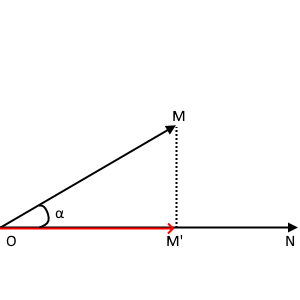
\includegraphics{resources/vector_axis_projection.png}
      \end{center}

      直接写出来:
      \begin{enumerate}
        \item $\projection{u}\vec{a} = |\vec{a}|\cdot\cos\alpha$
        \item $\projection{u}(\vec{a} + \vec{b}) = \projection{u}\vec{a} + \projection{u}\vec{b}$
        \item $\projection{u}\lambda\vec{a} = \lambda\projection{u}a$
      \end{enumerate}

      $u$:任意轴\qquad$\vec{a}$:向量\qquad$\projection{u}$:投影到u轴

    }%向量投影结尾

    \subsection{数量积/点乘}{
      点乘算出来的是数

      $\vec{a} \cdot \vec{b} = |a|\cdot|b|\cdot\cos\theta = |a|\cdot\projection{a}b = |b|\cdot\projection{b}a$

      $\theta$:夹角\\

      \indent点乘有以下性质:
      \begin{enumerate}
        \item $\vec{a}\cdot\vec{a} = |a|\cdot|a|\cdot\cos0 = |a|^2$
        \item $\vec{a}\cdot\vec{b} = 0,\theta = 90\degree,\vec{a} \perp \vec{b}$\qquad 即:$\vec{a}\cdot\vec{b} = 0 \Leftrightarrow \vec{a} \perp \vec{b}$
        \item $\vec{a}\cdot\vec{b} = \vec{b}\cdot\vec{a}$
        \item $(\vec{a}+\vec{b})\cdot\vec{c} = \vec{a}\cdot\vec{c} + \vec{b}\cdot\vec{c}$
        \item $(\lambda\vec{a})\cdot\vec{b} = \lambda(\vec{a}\cdot\vec{b})$
        \item $\vec{a} = (a_x,a_y,a_z),\vec{b} = (b_x,b_y,b_z),\vec{a}\cdot\vec{b} = a_xb_x + a_yb_y + a_zb_z$
        \item $\cos\theta = \cfrac{\vec{a}\cdot\vec{b}}{|\vec{a}|\cdot|\vec{b}|} = \cfrac{a_xb_x + a_yb_y + a_zb_z}{\sqrt{a_x^2 + a_y^2 + a_z^2}\cdot\sqrt{b_x^2 + b_y^2 + b_z^2}}$
      \end{enumerate}

    }%数量积/点乘结尾

    \subsection{向量积/叉乘}{
      叉乘算出来的是向量,这个向量垂直于其他两个向量.右手法则:食指为$\vec{a}$,中指为$\vec{b}$,拇指为$\vec{c}$

      $\vec{a}\times\vec{b} = \vec{c}$

      其中:$\vec{c}\perp\vec{a},\vec{c}\perp\vec{b}$\\

      \indent有以下性质:
      \begin{itemize}
        \item $\vec{a}\times\vec{a} = 0$
        \item 有非零向量$\vec{a},\vec{b},\vec{a}\times\vec{b} = 0\ \Rightarrow \vec{a} // \vec{b}$.即:$\vec{a} // \vec{b} \Leftrightarrow \vec{a} \times \vec{b} = 0$
        \item $\vec{b}\times\vec{a} = -\vec{b}\times\vec{a}$
        \item $(\vec{a} + \vec{b})\times\vec{c} = \vec{a} \times \vec{c} + \vec{b} \times \vec{c}$
        \item $(\lambda\vec{a})\times\vec{b} = \vec{a} \times (\lambda\vec{b}) = \lambda(\vec{a}\times\vec{b})$
      \end{itemize}

      有两种计算方法:

      首先,设$\vec{a} = (a_1,a_2,a_3),\vec{b} = (b_1,b_2,b_3)$,并将结果向量记作$\vec{s}$:

      \begin{itemize}
        \item {
              坐标形式:

              $$
                \vec{s}
                =
                \vec{a}\times\vec{b}
                =
                \begin{bmatrix}
                  s_1 \\
                  s_2 \\
                  s_3
                \end{bmatrix}
                =
                \begin{bmatrix}
                  a_2b_3 - a_3b_2 \\
                  a_3b_1 - a_1b_3 \\
                  a_1b_2 - a_2b_1
                \end{bmatrix}
              $$
              }
        \item {
              行列式形式:

              $$
                \vec{s}
                =
                \vec{a}\times\vec{b}
                =
                \left|\begin{array}{ccc}
                  \vec{i} & \vec{j} & \vec{k} \\
                  a_1     & a_2     & a_3     \\
                  b_1     & b_2     & b_3
                \end{array}\right|
              $$
              }
      \end{itemize}
    }%向量积/叉乘结尾

  }%关于向量结尾

  \section{关于圆}{

    \subsection{圆的方程}{
      \begin{center}
        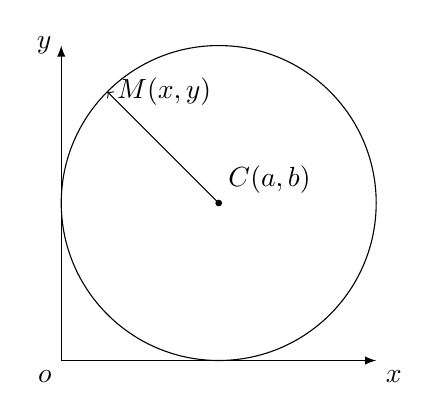
\begin{tikzpicture}
          \draw[-latex] (0,0) node[below left]{$o$} -- (4,0) node[below right]{$x$};
          \draw[-latex] (0,0) -- (0,4) node[left]{$y$};
          \draw  (2,2) circle (2);
          \tikzPlaceDot{(2,2) node [above right]{$C(a,b)$}};
          \draw[->] (2,2) -- ({2 - sqrt(2)},{2 + sqrt(2)}) node[right]{$M(x,y)$};
        \end{tikzpicture}
      \end{center}

      \begin{itemize}
        \item {
              圆的标准方程 : $(x - a)^2 + (y - b)^2 = r^2$

              由圆的定义可知,$\absoluteValue{\vec{CM}} = r$,因此 : $$
                \sqrt{(x - a)^2 + (y - b)^2} = r
              $$
              即,以$C(a,b)$为圆心,$r$为半径的圆的方程为 : $$
                (x - a)^2 + (y - b)^2 = r^2
              $$
              }
        \item {
              圆的一般方程 : $x^2 + y^2 + Dx + Ey + F = 0$

              将标准方程展开可得以上形式,反过来,也可以将以上形式配方,得到 : $$
                \bigCase{x + \cfrac{D}{2}}^2 + \bigCase{y + \cfrac{E}{2}}^2 = \cfrac{D^2 + E^2 - 4F}{4}
              $$

              \begin{enumerate}
                \item $D^2 + E^2 - 4F$称为圆方程的判别式,暂时把他记作$\alpha$吧(非正式用法,只在本章有效).
                \item 当$\alpha > 0$时,把一般方程和圆的标准方程比较,可以看出此一般方程表示以$\bigCase{-\cfrac{D}{2},-\cfrac{E}{2}}$为圆心,半径为$\cfrac{1}{2}\sqrt{D^2 + E^2 - 4F}$的圆.
                \item 当$\alpha = 0$时,方程只有一个实数解-也就是说方程只表示唯一的一个点$\bigCase{-\cfrac{D}{2},-\cfrac{E}{2}}$.
                \item 当$\alpha < 0$时,方程没有实数解,此时方程没有图形.
              \end{enumerate}

              因从,当$\alpha > 0$时,此种方程形式就叫做圆的一般方程,这种形式有以下特点 :
              \begin{enumerate}
                \item $x^2$与$y^2$的系数相同且不为0.
                \item 不含$xy$项.
                \item $D^2 + E^2 - 4F > 0$.
              \end{enumerate}
              }
      \end{itemize}
    }%圆的方程结尾

    \subsection{圆的切线方程}{
      已知$M(x_0,y_0)$为圆$x^2 + y^2 = r^2$上的一点,求过点$M$的圆$C$的切线$l$的方程 :

      因为$M$是$l$与圆$C$的切点,所以过$M$的半径$OM$与$l$垂直,即$\vec{OM}=\begin{bmatrix}
          x_0 \\ y_0
        \end{bmatrix}$是$l$的法向量,于是可得切线$l$的点法向式方程 : $$
        x_0(x - x_0) + y_0(y - y_0) = 0
      $$
      整理后可得 : $$
        x_0x + y_0y = x_0^2 + y_0^2
      $$
      又因为$M$在$C$上,因此$x_0^2 + y_0^2 = r^2$,最终得到切线的方程为 : $$
        x_0x + y_0y = r^2
      $$
    }%圆的切线方程结尾

  }%关于圆结尾

  \section{关于椭圆}{

    \subsection{椭圆的一般方程}{
      \begin{center}
        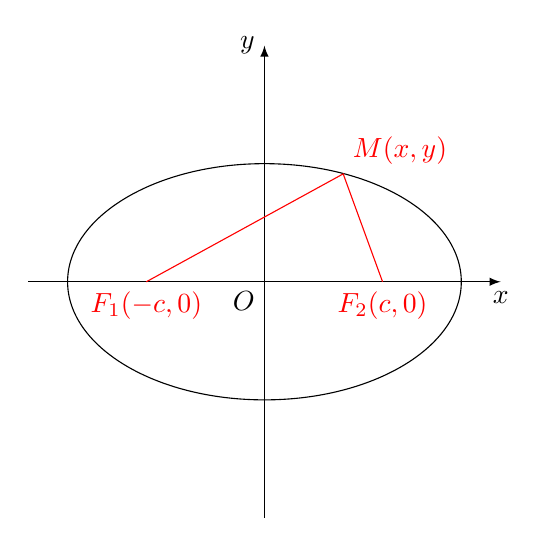
\begin{tikzpicture}
          \draw[-latex] (-3,0) -- node[below left]{$O$} (3,0)node [below]{$x$};
          \draw[-latex] (0,-3) -- (0,3)node [left]{$y$};
          \draw (0,0) ellipse (2.5 and 1.5);
          \draw[red] (1.5,0) node[below]{$F_2(c,0)$} -- (1,1.37) node[above right]{$M(x,y)$} -- (-1.5,0) node[below]{$F_1(-c,0)$};
        \end{tikzpicture}
      \end{center}

      将平面内到两个定点$F_1,F_2$的距离之和等于常数$2a$的点的轨迹叫做椭圆.这两个定点叫做椭圆$EC$的焦点,两个焦点的距离$\absoluteValue{F_1F_2}$称为椭圆的焦距.

      根据定义,建系建立方程,设焦距为$2c$,$F_1,F_2$的坐标分别为$(-c,0),(c,0)$.设$M(x,y)$是椭圆上任意一点,点$M$到两焦点的距离和等于$2a(a>c>0)$. : $$
        \absoluteValue{MF_1} + \absoluteValue{MF_2} = \sqrt{(x + c)^2 + y^2} + \sqrt{(x - c)^2 + y^2} = 2a
      $$
      将第二项移到右边,两边平方再整理,得 : $$
        a^2 - cx = a\sqrt{(x - c)^2 + y^2}
      $$
      两边再平方,经过整理,得 : $$
        (a^2 - c^2)x^2 + a^2y^2 = a^2(a^2 - c^2)
      $$
      由于$a^2 - c^2 > 0$,设$吧^2 = a^2 - c^2$ : $$
        b^2x^2 + a^2y^2 = a^2b^2
      $$
      即 : $$
        \cfrac{x^2}{a^2} + \cfrac{y^2}{b^2} = 1(a>b>0)
      $$
      同理,如果焦点在y轴上,那么方程就是 : $$
        \cfrac{y^2}{a^2} + \cfrac{x^2}{b^2} = 1(a > b > 0)
      $$

      这其实是一种很漂亮的形式 :

      \begin{center}
        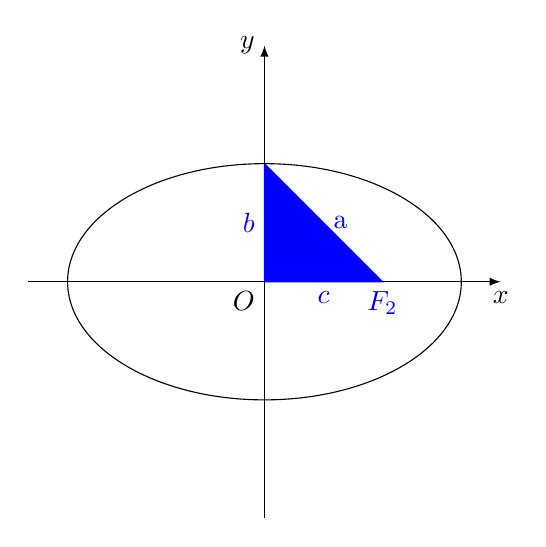
\begin{tikzpicture}
          \draw[-latex] (-3,0) -- node[below left]{$O$} (3,0)node [below]{$x$};
          \draw[-latex] (0,-3) -- (0,3)node [left]{$y$};
          \draw (0,0) ellipse (2.5 and 1.5);
          \filldraw[blue] (1.5,0) node[below]{$F_2$} -- node[below]{$c$} (0,0) -- node[left]{$b$}(0,1.5) -- node[right]{a} cycle;
        \end{tikzpicture}
        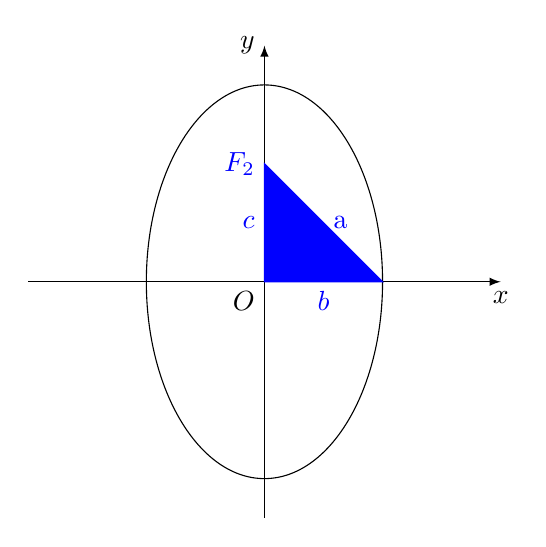
\begin{tikzpicture}
          \draw[-latex] (-3,0) -- node[below left]{$O$} (3,0)node [below]{$x$};
          \draw[-latex] (0,-3) -- (0,3)node [left]{$y$};
          \draw (0,0) ellipse (1.5 and 2.5);
          \filldraw[blue] (0,1.5) node[left]{$F_2$} -- node[left]{$c$} (0,0) -- node[below]{$b$}(1.5,0) -- node[right]{a} cycle;
        \end{tikzpicture}
      \end{center}

      这就是椭圆的标准方程.
    }%椭圆的一般方程结尾

  }%关于椭圆结尾

  \section{关于空间平面}{

    \subsection{空间平面公式}{
      法线向量与平面垂直.\\

      \indent空间平面有以下表示方法:
      \begin{itemize}
        \item {
              点法式:知道一点与法线向量.

              设一点$M_0:(x_0,y_0,z_0)$,法线向量:$\vec{n} = (A,B,C)$

              设$M(x,y,z),\vec{M_0M}=(x - x_0,y - y_0,z - z_0),\vec{n} \cdot \vec{M_0M} = 0$

              平面的点法式方程为:$A(x - x_0) + B(y - y_0) + C(z - z_0) = 0$
              }
        \item {
              一般式:三点确定一个向量.以实例演示:

              设$M_1(2,-1,4),M_2(-1,3,-2),M_3(0,2,3)$代入:

              $Ax + By + Cz + D = 0$

              $$
                \begin{cases}
                  2A - B + 4C = -D \\
                  -A + 3B -2C = -D \\
                  2B + 3C = -D
                \end{cases}
              $$

              也有$Ax + By + Cz + (-Ay_0 - By_0 - Cz_0) = 0$

              (由点法式推出)\\

              \indent有以下情况:
              \begin{enumerate}
                \item $D = 0,Ax + By + Cz = 0$:平面过原点.
                \item $A = 0,By + Cz + D = 0$:法线垂直与$x$轴且平面平行于$x$轴,类似情况同理
                \item $A = B = 0,CZ + D = 0$:平面过$z = -\cfrac{D}{C}$,平行于$xy$轴.
              \end{enumerate}
              }
        \item 截距式:$\cfrac{x}{a} + \cfrac{y}{b} + \cfrac{z}{c} = 1$
      \end{itemize}
    }%关于空间平面结尾

    \subsection{求两平面夹角}{
      其实是求两平面法线的夹角(取锐角)

      因此只要设两平面法线向量为$n_1(A_1,B_1,C_1),n_2(A_2,B_2,C_2)$,然后套向量夹角公式就行了.

      其中$\theta = (\widehat{n_1\ n_2})$或$(\widehat{-n_1\ n_2}) = (\pi - (\widehat{n_1\ n_2}))$

      其中当向量平行时意味着平面重合(因为取的是锐角)、
    }%求两平面夹角结尾

    \subsection{点到平面距离公式}{
      设点$P_0(x_0,y_0,z_0),Ax + By + Cz + D = 0$

      $d = \cfrac{|Ax_0 + By_0 + Cz_0 + D|}{\sqrt{A^2 + B^2 + C^2}}$
    }%点到平面距离公式结尾

    \subsection{直线与平面夹角}{
      指的是直线与法线的夹角

      设与直线同方向的向量$L_1(M,N,P)$,夹角为$\theta$

      $\sin\theta = \cfrac{|AM + BN + CP|}{\sqrt{A^2 + B^2 + C^2}\sqrt{M^2 + N^2 + P^2}}$\\

      \indent有以下几种情况:
      \begin{enumerate}
        \item 直线垂直于平面: $\cfrac{A}{M} = \cfrac{B}{N} = \cfrac{C}{P}$
        \item 直线平行于平面: $AM + BN + CP = 0$
      \end{enumerate}
    }%直线与平面夹角结尾

  }%空间平面及其方程结尾

  \section{关于空间直线}{

    \subsection{空间直线及其方程}{
      有以下三种形式:

      \begin{enumerate}
        \item {
              一般方程:(即两平面的交线)

              $$
                \begin{cases}
                  A_1x + B_1y + C_1Z + D_1 = 0 \\
                  A_2x + B_2y + C_2z + D_2 = 0
                \end{cases}
              $$
              }
        \item {
              对称式方程:

              设点$M(x,y,z),M_0(x_0,y_0,z_0)$是直线$L$上的任意两点,那么存在向量$\vec{M_0M}$与直线$L$的方向向量$\vec{s}$平行.因此两向量的对应坐标成比例.$(\vec{M_0M} = (x - x_0, y - y_0, z - z_0), \vec{s} = (m,n,p))$,因此得出:

              $\cfrac{x - x_0}{m} = \cfrac{y - y_0}{n} = \cfrac{z - z_0}{p} = t$
              }
        \item {
              参数式:将对称式变形

              $$
                \begin{cases}
                  x = x_0 + mt \\
                  y = y_0 + nt \\
                  z = z_0 + pt
                \end{cases}
              $$
              }
      \end{enumerate}
    }%空间直线及其方程结尾

    \subsection{平面束}{
      平面束即形成一条直线的所有面

      $$
        \begin{cases}
          A_1x + B_1y + C_1z + D_1 = 0 \\
          A_2x + B_2y + C_2z + D_2 = 0
        \end{cases}
      $$

      其中$A_1,B_1,C_1$与$A_2,B_2,C_2$不成比例.即:$A_1x + B_1y + C_1z + D_1 + \lambda(A_2x + B_2y + C_2z + D_2) = 0, (\lambda \in \mathRealNumberCollection)$
    }%平面束结尾

  }%关于空间直线结尾

  \section{关于空间曲线}{

    \subsection{空间曲线及其方程}{
      有以下两种形式:

      \begin{enumerate}
        \item {
              一般式:(两曲面的交线)

              $$
                \begin{cases}
                  F(x,y,z) = 0 \\
                  G(x,y,z) = 0
                \end{cases}
              $$
              }
        \item {
              参数方程:(将曲线上的动点的坐标表示为参数t的函数)

              $$
                \begin{cases}
                  x = x(t) \\
                  y = y(t) \\
                  z = z(t)
                \end{cases}
              $$
              }
      \end{enumerate}
    }%空间曲线及其方程结尾

    \subsection{参数方程与一般方程的互化}{
      这两者之间的互化往往会用到一些特殊的技巧,比如诱导公式.

      举例 : 设一个圆的参数方程为 : $$
        \begin{cases}
          x = -1 + \cos \theta \\
          y = 3 + \sin \theta
        \end{cases}
        \mbox{($\theta$是参数)}
      $$

      仅列出以下解法 :
      \begin{enumerate}
        \item {
              利用平方关系$\cos^2\theta + \sin^2\theta = 1$,先将原方程整理一下 : $$
                \begin{cases}
                  \cos\theta = x + 1 \\
                  \sin\theta = y - 3
                \end{cases}
              $$
              代入得 : $$
                (x + 1)^2 + (y - 3)^2 = 1
              $$
              }
        \item {
              类比圆的参数方程形式 : $$
                \begin{cases}
                  x = x_0 + r\cos\alpha \\
                  y = y_0 + r\sin\alpha
                \end{cases}
              $$

              可知圆心为$(-1,3)$,半径$r = 1$,所以普通方程为 : $$
                (x + 1)^2 + (y - 3)^2 = 1
              $$
              }
      \end{enumerate}

      关键在于如何利用一般情况下的公式的结构,而且需要明确参数和角度的区别(因为往往$\theta$是被看作参数而非角度).
    }%参数方程与一般方程的互化结尾

    \subsection{常见参数方程}{
      以下都是二维参数方程.

      \begin{itemize}
        \item {
              直线 :
              \begin{itemize}
                \item 点斜式 : 过$(x_0,y_0)$,斜率为$m$的直线 : $\begin{cases}
                          x = x_0 + y \\
                          y = y_0 + mt
                        \end{cases}$
                \item 点向式 : 过$(x_0,y_0)$,方向向量为$(u,v)$的直线 : $\begin{cases}
                          x = x_0 + ut \\
                          y = y_0 + vt
                        \end{cases}$
              \end{itemize}
              }
        \item 圆 : $\begin{cases}
                  x = r\cos t \\
                  y = r\sin t
                \end{cases}$
        \item 椭圆 : $\begin{cases}
                  x = a\cos t \\
                  y = b\sin t
                \end{cases}$
        \item 双曲线 : $\begin{cases}
                  x = a\sec t \\
                  y = b\tan t
                \end{cases}$
        \item 抛物线 : $\begin{cases}
                  x = 2ct \\
                  y = t^2
                \end{cases}$
        \item 螺线 : $\begin{cases}
                  x = t\cos lt \\
                  y = t\sin lt
                \end{cases}$
        \item 摆线 : $\begin{cases}
                  x = r \cdot (t - \sin t) \\
                  y = r \cdot (1 - \cos t)
                \end{cases}$
      \end{itemize}

      注 : 上文中的$a,b,c,h,k,l,m,p,r,x_0,y_0,u,v$为已知数,$t$都是参数,$x,y$为一般方程下的变量.
    }%常见参数方程结尾

    \subsection{空间曲线在坐标系面上的投影}{

      设空间曲线c的一般方程为:

      $$
        \begin{cases}
          F(x,y,z) = 0 \\
          G(x,y,z) = 0
        \end{cases}
      $$

      消去其中一个变量,(比如z),求在xoy上的投影,得到方程:

      $$
        \begin{cases}
          F(x,y) = 0 \\
          z = 0
        \end{cases}
      $$
    }%空间曲线在坐标系面上的投影结尾

    \subsection{空间曲线的切线及法平面}{
      先写出空间曲线的切线方程 :

      $$
        \begin{cases}
          x = \varphi(t) \\
          y = \Phi(t)    \\
          z = \omega(t)
        \end{cases}
      $$

      其中 $t \in [\alpha,\beta]$,设三个函数都可导且不同时为0.

      则切向量$\vec{T} = \begin{bmatrix}
          \varphi\derivative(t_0) & \Phi\derivative(t_0) & \omega\derivative(t_0)
        \end{bmatrix}$

      切线方程为 : $\cfrac{x - x_0}{\varphi\derivative(t_0)} = \cfrac{y - y_0}{\Phi\derivative(y_0)} = \cfrac{z - z_0}{\omega\derivative(t_0)}$

      则法平面的点法式方程为 : $\varphi\derivative(t_0)(x - x_0) + \Phi\derivative(t_0)(y - y_0) + \omega\derivative(z - z_0) = 0$
    }%空间曲线的切线及法平面

    \subsection{空间曲线的切平面及法线}{
      有两种情况 :

      \begin{enumerate}
        \item {
              $F(x,y,z) = 0$(即隐函数)

              则切平面的方程为:$F\derivative_x(x_0,y_0,z_0)(x - x_0) + F\derivative_y(x_0,y_0,z_0)(y - y_0) + F\derivative_z(x_0,y_0,z_0)(z - z_0) = 0$

              法线的方程为 : $\cfrac{x - x_0}{F\derivative_x(x_0,y_0,z_0)} = \cfrac{y - y_0}{F\derivative_y(x_0,y_0,z_0)} = \cfrac{z - z_0}{F\derivative_z(x_0,y_0,z_0)}$
              }
        \item {
              $z = \defFunction{x,y}$,只需让$F = \defFunction{x,y} - z$,然后套公式1.

              切平面解析式为 : $f\derivative_x(x_0,y_0)(x - x_0) + f\derivative_y(x_0,y_0)(y - y_0) - (z - z_0) = 0$
              }
      \end{enumerate}
    }%空间曲线的切平面及法线

  }%关于空间曲线结尾

  \section{关于空间曲面}{

    \subsection{空间曲面及其方程}{
      有非常多种曲面,都给他列出来:

      \begin{itemize}
        \item {
              旋转曲面:由二次曲线绕某一坐标轴旋转形成.

              \begin{itemize}
                \item {
                      设YOZ平面上有曲线$\defFunction{y,z} = 0$:

                      \begin{itemize}
                        \item 绕z轴旋转,曲面表达式为:$\defFunction{\pm\sqrt{x^2 + y^2},z} = 0$
                        \item 绕y轴旋转,曲面表达式为:$\defFunction{y,\pm\sqrt{x^2 + z^2}} = 0$
                      \end{itemize}
                      }
                \item {
                      设XOY平面上有曲线$\defFunction{x,y} = 0$:

                      \begin{itemize}
                        \item 绕x轴旋转,曲面表达式为:$\defFunction{x,\pm\sqrt{y^2 + z^2}} = 0$
                        \item 绕y轴旋转,曲面表达式为:$\defFunction{\pm\sqrt{x^2 + z^2},y} = 0$
                      \end{itemize}
                      }
                \item {
                      设XOZ平面上有曲线$\defFunction{x,z} = 0$:

                      \begin{itemize}
                        \item 绕x轴旋转,曲面表达式为:$\defFunction{x,\pm\sqrt{y^2 + z^2}} = 0$
                        \item 绕z轴旋转,曲面表达式为:$\defFunction{\pm\sqrt{x^2 + y^2},z} = 0$
                      \end{itemize}
                      }
              \end{itemize}
              }
        \item {
              二次曲面:

              二次曲面有以下12种:
              \begin{itemize}
                \item {
                      椭球面:

                      在直角坐标系中的方程为:

                      $\cfrac{x^2}{a^2} + \cfrac{y^2}{b^2} + \cfrac{z^2}{c^2} = 1$

                      其中a和b是赤道半径(沿着x和y轴),c是极半径,(沿着z轴).这三个数都是固定的正实数,决定了椭球的形状.

                      如果三个半径都是相等的,那么就是一个球;如果有两个半径是相等的,则是一个类球面.

                      \begin{itemize}
                        \item $a = b = c$:球
                        \item $a = b > c$:扁球面
                        \item $a = b < c$:长球面
                        \item $a \neq b,b \neq c,c \neq a$:不等边椭球(三条边都不相等)
                      \end{itemize}

                      点(a,0,0)、(0,b,0)和(0,0,c)都在曲面上.从原点到这三个点的线段,称为椭球的半主轴.它们与椭圆的半长轴和半短轴相对应.

                      体积公式为:$\cfrac{4}{3}\pi abc$.

                      注意,当三个半径都相等时,这个公式便化为球的体积;两个半径相等时,便化为扁球面或长球面的体积.
                      }
                \item {
                      抛物面:

                      例:$y^2 - 2x = 0 / F(x,y) = 0$,参数中缺少z,因此母线平行于z轴
                      }
                \item {
                      椭圆抛物面:

                      椭圆抛物面在直角坐标系中的方程为:$z = \cfrac{x^2}{a^2} + \cfrac{y^2}{b^2}$
                      }
                \item {
                      双曲抛物面:

                      双曲抛物面在直角坐标系中的方程为:$z = \cfrac{x^2}{a^2} - \cfrac{y^2}{b^2}$
                      }
                \item {
                      单叶双曲面:

                      单叶双曲面在直角坐标系中的方程为:$\cfrac{x^2}{a^2} + \cfrac{y^2}{b^2} - \cfrac{z^2}{c^2} = 1$

                      当a = b时双曲面就会变得比较圆
                      }
                \item {
                      双叶双曲面:

                      双叶抛物面在直角坐标系中的方程为:$\cfrac{x^2}{a^2} + \cfrac{y^2}{b^2} - \cfrac{z^2}{c^2} = -1$

                      当a = b时双曲面就会变得比较圆
                      }
                \item {
                      类球面:

                      类球面是一种二次曲面.二维的椭圆有两个主轴,称为长轴与短轴.在三维空间里,将一个椭圆绕着其任何一主轴旋转,则可得到一个类球面.

                      \begin{itemize}
                        \item 假若,这旋转主轴是长轴,则这个类球面为长球面.例如,英式足球里所用的橄榄球是长球形状.
                        \item 假若,这旋转主轴是短轴,则这个类球面为扁球面.例如,地球在北极与南极稍微有点扁平,在赤道又有点凸涨.所以,地球是扁球形状.
                        \item  假若,生成的椭圆是圆圈,则这个类球面为完全对称的圆球面.
                      \end{itemize}

                      用另一种方法来描述,类球面是一种椭球面.而椭球面的公式已经给出,其中a与b分别是椭球面在x轴与y轴的赤道半径,c是椭球面在z轴的极半径,这三个正实数的半径决定了椭球面的形状.以z轴为旋转轴的类球面a = b,他的方程为:

                      $\cfrac{x^2 + y^2}{a^2} + \cfrac{z^2}{c^2} = 1$

                      \begin{itemize}
                        \item 如果三个半径都相等,则此椭球面是圆球面$(a = c)$
                        \item 如果类球面的赤道半径小于极半径,则这是类球面中的长球面.$(a < c)$
                        \item 如果类球面的赤道半径大于极半径,则这是类球面中的扁球面.$(a > c)$
                      \end{itemize}
                      }
                \item {
                      球面:

                      在空间解析几何中,球心为$(x_0,y_0,z_0)$,半径为r的球面是满足以下方程的所有点的轨迹:

                      $(x - x_0)^2 + (y - y_0)^2 + (z - z_0)^2 = r^2$

                      当球心在原点上:$x^2 + y^2 + z^2 = r^2$

                      可化作三元二次方程:$Ax^2 + Ay^2 + Az^2 + Bx + Cy + Dz + G = 0$(平方项系数相同)

                      其中$D^2 + E^2 + F^2 > 4AG$.

                      当满足以上两点时可逆推出一个三元二次方程是否为一个球面

                      (当$D^2 + E^2 + F^2 = 4AG$时是一个点)
                      }
                \item {
                      椭圆锥面(二次锥面):

                      椭圆锥面在直角坐标系中的方程为:$\cfrac{x^2}{a^2} + \cfrac{y^2}{b^2} - \cfrac{z^2}{c^2} = 0$

                      当a = b时就会变成圆锥面.
                      }
                \item {
                      椭圆柱面:

                      椭圆柱面在直角坐标系中的方程为:$\cfrac{x^2}{a^2} + \cfrac{y^2}{b^2} = 1$

                      当a = b时就会变成圆柱面.
                      }
                \item {
                      双曲柱面:

                      双曲柱面在直角坐标系中的方程为:$\cfrac{x^2}{a^2} - \cfrac{y^2}{b^2} = 1$
                      }
                \item {
                      抛物柱面:

                      抛物柱面在直角坐标系中的方程为:$x^2 + 2ay = 0$
                      }
              \end{itemize}
              }
      \end{itemize}
    }%空间曲面及其方程结尾

    \subsection{伸缩法}{
      注:伸缩法不是放缩法!

      举例:有$x^2 + y^2 = 1$,沿着y轴伸缩两倍,则伸缩后的方程为:$x^2 + \cfrac{y^2}{4} = 1$.

      也就是说:沿着n轴伸缩,就对变量n进行替换.

      伸缩t倍,就把原变量替换成$\cfrac{n}{t}$
    }%伸缩法结尾
  }%关于空间曲面结尾

 }%解析几何结尾
  %*数学分析_1
  %\section{微积分}{

\subsection{极限}{

  \subsubsection{定理}{
    \begin{enumerate}
      \item 函数在一点极限存在的条件是左右极限存在且相等
      \item 洛必达法则:当极限为$\cfrac{0}{0}$或者$\cfrac{\infty}{\infty}$时可上下同时求导,求导后极限不变,每一步都需要重新判断是否依然符合类型
      \item {
            归结原则(海涅定理\#狭义) :

            $\limNormal{x \to a}\defFunction{x} = b$存在的充要条件是:

            取$\defFunction{x}$定义域内的任意数列${a_n}$,$\limNormal{n \to \infty}a_n = a$,且$a_n$不等于$a$,则$\limNormal{n \to \infty}\defFunction{a_n} = b$.

            海涅定理表明了函数极限与数列极限的关系.如果极限$\limNormal{x \to x_0}\defFunction{x}$存在,${x_n}$为函数$\defFunction{x}$定义域内任一收敛于$x_0$的数列,且满足 : $x_n \neq x_0,n \in \mathNatureNumberCollection^+$,那么相应的函数值数列${\defFunction{x_n}}$必收敛,且$\limNormal{n \to \infty}\defFunction{x_n} = \limNormal{x \to x_0}\defFunction{x}$.
            }
    \end{enumerate}
  }%极限定理结尾

  \subsubsection{重要极限}{
    $\myLimToZero\cfrac{\sin{x}}{x}=1 \to \limNormal{x \to 0}\sin{x} \to x$

    $\myLimToInf(1+\cfrac{1}{x})^x = e$
  }%重要极限结尾  

  \subsubsection{等价无穷小}{
    $\myLimToZero a^x - 1 \approx x\ln{a}$

    $\myLimToZero \arcsin(a)x \approx \sin(a)x \approx (a)x$

    $\myLimToZero \arctan(a)x \approx \tan(a)x \approx (a)x$

    $\myLimToZero \ln1+x \approx x$

    $\myLimToZero e^x \approx 1+x$

    $\myLimToZero \sqrt{1 + x} - \sqrt{1 - x} \approx x$

    $\myLimToZero \tan{x} \approx x$

    $\myLimToZero (1 + ax)^b - 1 \approx abx$

    $\myLimToZero (1+x)^\alpha \approx 1+\alpha x$

    $\myLimToZero 1 - \cos x \approx \cfrac{x^2}{2}$

    $\myLimToZero x - \ln(1 + x) \approx \cfrac{x^2}{2}$

    $\myLimToZero \tan x - x \approx \cfrac{x^3}{3}$

    $\myLimToZero x - \arctan x \approx \cfrac{x^3}{3}$

    $\myLimToZero x - \sin x \approx \cfrac{x^3}{6}$

    $\myLimToZero \arcsin x - x \approx \cfrac{x^3}{6}$

    以上等价无穷小都可以由泰勒公式推出
  }%等价无穷小结尾

}%极限结尾

\subsection{数列极限相关}{

  注:本章内容可用于级数.

  注:数列不是级数,级数需要求和数列不用.

  \subsubsection{数列}{
    若函数$f$的定义域为全体正整数集合$\mathNatureNumberCollection^n$,则称
    $$
      f : \mathNatureNumberCollection^+ \to \mathRealNumberCollection,\defFunction{n} \ (n \in \mathNatureNumberCollection^+)
    $$

    为数列.因正整数集$\mathNatureNumberCollection^+$的元素可按由小到大的顺序排列,所以数列$\defFunction{n}$也可以写作 :
    $$
      a_1,a_2,a_3,\dots,a_n,\dots,
    $$

    或者可以简记为${a_n}$,其中$a_n$称为该数列的通项.
  }%数列结尾

  \subsubsection{数列极限}{
    设数列${a_n}$,存在$a_0$,若对于任意给定的正数$\epsilon$,总存在正整数$N$,使得当$n > N$时由
    $$
      \absoluteValue{a_n - a} < \epsilon
    $$

    则称数列${a_n}$收敛于$a,a$称为数列$a_n$的极限,记作
    $$
      \limNormal{n \to \infty}a_n = a
    $$

    若数列${a_n}$没有极限,则称${a_n}$不收敛,或者称${a_n}$发散.

    此定义等价于 : 任给$\epsilon > 0$,若在$(a - \epsilon,a + \epsilon)$之外数列${a_n}$中的项至多只有有限个,则称数列${a_n}$收敛域极限$a$.
  }%数列极限结尾

  \subsubsection{O'Stolz(stolz)定理}{
    设$(a_n)_{n > 1}$和$(b_n)_{n > 1}$为两个实数数列.若$b_n$为从某项开始严格单调的无界正数数列,且有穷极限
    $$
      \limNormal{n \to \infty}\cfrac{a_{n + 1} - a_n}{b_{n + 1} - b_n} = L
    $$

    存在,则 :
    $$
      \limNormal{n \to \infty}\cfrac{a_n}{b_n} = L
    $$

    其中$L$可以为有限实数或正/负无穷.

    该定理虽然主要被用于处理数列不定型极限,但该定理再没有$\limNormal{n \to \infty}a_n = \infty$这一条件时也是成立的.虽然该定理通常是以分布$b_n$为正数数列的情形加以叙述的,但注意到该定理对分子$a_n$的正负没有限制,所以原则上把对数列$b_n$的限制条i按替换为"严格单调递减且趋于负无穷大"也是没问题的.

    与洛必达的迭代用法类似,在尝试使用此定理考察数列极限时,如果发现两个数列差分的商任然是不定型,那么可以继续用.

    注意 : 与洛必达类似,判定条件不存在不能认定极限本身不存在.
  }%O'Stolz(stolz)定理结尾

}%数列极限相关结尾

\subsection{渐进线}{
  渐近线分为三种 :
  \begin{itemize}
    \item 水平渐近线 : 当$x \to x_0$时,$\myLimToInf\defFunction{x} = y_0$,则$y = y_0$是水平渐近线.
    \item 垂直渐近线 : 当$x \to x_0$时,$\limNormal{x \to x_0}\defFunction{x} \to \infty$,且$x_0$为一般间断点,则$x = x_0$是垂直渐近线.
    \item {
          斜渐近线 :

          当$\myLimToInf\left[\defFunction{x} - (ax + b)\right] = 0(a,b \in \mathConstant)$存在,则$y = ax + b$是斜渐近线.

          即 : 如果$\myLimToInf\cfrac{\defFunction{x}}{x} = a$存在,且$\myLimToInf\left[\defFunction{x} - ax\right] = b$也存在,则$y = \defFunction{x}$有斜渐近线$y = ax + b$
          }
  \end{itemize}
}%渐近线结尾

\subsection{导数}{
  导数是什么?教科书上普遍给出的定义是指:函数图像的斜率变化率曲线,事实上某些观点表示导数也可以理解成是函数对于输入值的敏感程度,即:输入值的变化对应的输出值的变化的剧烈程度.

  导数在一元情况下的定义是指$\limNormal{x to x_0}\cfrac{f(x) - f(x_0)}{x - x_0}$\ 或者\ $\limNormal{\Delta x \to x_0}\cfrac{f(x + \Delta x) - f(x)}{\Delta x}$

  值得注意的是:求导是一种线性运算.

  \subsubsection{求导法则}{
    以下为求导的基本法则:
    \begin{enumerate}
      \item $(u + v)\derivative = u\derivative + v\derivative$
      \item $(u - v)\derivative = u\derivative - v\derivative$
      \item $(uv)\derivative = u\derivative v + uv\derivative$
      \item $(uvw)\derivative = u\derivative vw + uv\derivative w + uvw\derivative$
      \item $(\mathbf{c}v)\derivative = \mathbf{c}(v)\derivative$
      \item $\cfrac{u}{v}\derivative = \cfrac{u\derivative v - uv\derivative}{v^2}$
    \end{enumerate}
    注:反函数的导数等于函数导数的倒数,即——互为倒数的导数相乘依然为1
  }%求导法则结尾

  \subsubsection{复合函数求导}{
    对于复合函数求导,有以下方法:

    $y = \fint(u), u = g(x); \cfrac{dy}{dx} = \cfrac{dy}{du} \cdot \cfrac{du}{dx} = f\derivative(u) \cdot g\derivative(x)$
  }%复合函数求导结尾

  \subsubsection{求导公式表}{
    以下为基本函数的求导公式表,类似线性组合,大多数函数的导数可以由以下公式组合得到.

    $\fint(x) = C, \fint\derivative(x) = 0$

    $\fint(x) = x^n, \fint\derivative(x) = nx^{n-1}$

    $\fint(x) = x, \fint\derivative(x) = 1$

    $\fint(x) = \sin x, \fint\derivative(x) = \cos x$

    $\fint(x) = \cos x, \fint\derivative(x) = -\sin x$

    $\fint(x) = \tan x, \fint\derivative(x) = \sec^2 x$

    $\fint(x) = \sec x, \fint\derivative(x) = \sec x\tan x$

    $\fint(x) = \cot x, \fint\derivative(x) = -\csc^2 x$

    $\fint(x) = \csc x, \fint\derivative(x) = -\csc x\cot x$

    $\fint(x) = \arcsin x, \fint\derivative(x) = \cfrac{1}{\sqrt{1 - x^2}}$

    $\fint(x) = \arccos x, \fint\derivative(x) = -\cfrac{1}{\sqrt{1 - x^2}}$

    $\fint(x) = \arctan x, \fint\derivative(x) = \cfrac{1}{1 + x^2}$

    $\fint(x) = arccotx, \fint\derivative(x) = -\cfrac{1}{1 + x^2}$

    $\fint(x) = a^x, \fint\derivative(x) = a^x\ln x$

    $\fint(x) = \log_a x, \fint\derivative(x) = \cfrac{1}{x\ln a}$

    $\fint(x) = \ln x, \fint\derivative(x)= \cfrac{1}{x}$

    $\fint(x) = e^x, \fint\derivative(x) = e^x$
  }%求导公式表结尾
  \newline

  值得注意的是:
  \begin{enumerate}
    \item 在一维的情况下,可导 $\Leftrightarrow$ 左右导数存在且相等

    \item 可导 $\Rightarrow$ 连续

    \item 连续则不一定可导
  \end{enumerate}

  \subsubsection{线性近似/牛顿法近似函数/求方程解}{
    由导数的另一种定义:$\fDerivative{x} = \limNormal{x \to a}\cfrac{\defFunction{x} - \defFunction{a}}{x - a}$

    当不再取极限的时候等号变成约等于,即:$\fDerivative{x} \approx \cfrac{\defFunction{x} - \defFunction{a}}{x - a}$, 两边移项,可得

    $\defFunction{x} \approx \defFunction{a} + (x-a)\fDerivative{a}$或者$x - a \approx -\cfrac{\defFunction{a}}{\fDerivative{a}}$

    前者被称为线性近似,后者就是牛顿法,其实本质上是同一个公式的不同变形.

    当x和a取值越接近,近似也就越精确,这种方法本质上是取级数展开形式的前两位.

  }%线性近似/牛顿法近似函数/方程解结尾

}%导数结尾

\subsection{偏导数}{

  设$\defFunction{x,y,z} = ax + by + cy + d$

  $\fint\partialDerivative{x}(x,y,z) = a$

  $\fint\partialDerivative{y}(x,y,z) = b$

  $\fint\partialDerivative{z}(x,y,z) = c$

  换言之,偏导就是只把要求偏导的变量看作变量,其他变量看作常量再求导.

  \subsubsection{全微分}{

    $\Delta z = \defFunction{x + \Delta x,y + \Delta y} - \defFunction{x,y}\qquad\Delta z : $ 近似求得

    定义:$\defFunction{x,y}$在定义域内有定义,产生$\Delta x$和$\Delta y$,$\Delta z = \defFunction{x + \Delta x,y + \Delta y} - \defFunction{x,y} = A\Delta x + B\Delta y + O(\rho)$

    其中$A = f\partialDerivative{x}, B = f\partialDerivative{y}, \rho = \sqrt{(\Delta x)^2 + (\Delta y)^2}$

    并且$A,B$是$x$和$y$的函数(此处$x,y$为常量),与$\Delta x$和$\Delta y$(此处$\Delta x, \Delta y$是变量)无关.

    如果能写成此形式,则称此函数在这点可微,且$A\Delta x + B\Delta y$叫做他的全微分.

    记作:$dz$(近似值)$= A\Delta x + B\Delta y \approx \Delta z$(精确值)

    注意 :

    \begin{itemize}
      \item 可微的必要条件 : 如果$z = f(x,y)$可微,可以推出偏导存在,且$dz - f\partialDerivative{x}\Delta x + f\partialDerivative{y}\Delta y$
      \item 可微的充分条件 : 在定义域内有连续偏导数.
    \end{itemize}
  }

}%偏导数结尾

\subsection{微分}{
那么微分(differential)又是什么?微分是一个函数在自变量做无穷小变化时函数值的变化.在形式上确实与导数类似,但不应该与导数混淆.

可以形象化理解,微分就是曲线的切线.给定一个横坐标,可以在切线上找到纵坐标.就是这样一个映射.而导数就是这条切线的斜率.

\subsubsection{微分公式}{
  给出以下微分公式,与导数确实类似,但微分和导数是两个不同的映射.他们的定义域都是可微函数,微分的值域是1-form,导数的值域是函数.
  \begin{enumerate}
    \item $d(u \pm v) = du \pm dv$
    \item $d(\mathbf{C}u) = \mathbf{c}du$
    \item $d(uv) = vdu + udv$
    \item $d(\cfrac{u}{v} = \cfrac{vdu + udv}{v^2})$
  \end{enumerate}
}%微分公式结尾

\subsubsection{复合微分}{
  与复合求导类似:

  $y = \fint(u), u = g(x);$

  $dy = y\derivative dx = \fint\derivative(u)du = \fint\derivative{u}g\derivative(x)dx$

  即:$du = dg(x)$
}%复合微分结尾

\subsubsection{罗尔中值定理}{
  \begin{center}
    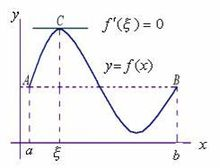
\includegraphics{resources/Rolle's_mean_value_theorem.jpg}
  \end{center}

  如果函数$\fint(x)$满足:

  \begin{enumerate}
    \item 在闭区间$[a,b]$上连续;
    \item 在开区间$(a,b)$上可导;
    \item 在区间端点处的函数值相等,即$\fint(a) = \fint(b)$,
  \end{enumerate}

  那么在$(a,b)$内至少有一点$\xi, (a<\xi<b)$,使得$\fint\derivative(\xi) = 0$.这个定理称为罗尔定理
}%罗尔中值定理结尾

\subsubsection{拉格朗日中值定理}{
\begin{center}
  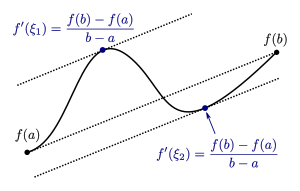
\includegraphics{resources/Lagrange's_mean_value_theorem.png}
\end{center}

令$\fint : [a,b] \to \mathbf{R}$为闭区间$[a,b]$上的一个函数,且在开区间
$(a,b)$内对任意一点$x$,极限$\limNormal{h \to 0}\cfrac{\fint(x + h) - \fint(x)}{h}$存在,
为一个有限数字或者等于$+\infty$或$-\infty$.如果有限,则极限等于$\fDerivative{x}$.

此定理称为{\bfseries拉格朗日中值定理},也简称中值定理,是罗尔中值定理的更一般的形式,同时也是柯西中值定理的特殊情形

这个定理再可以稍微推广一点.只需假设$\fint : [a,b] \to \mathbf{R}$在$[a,b]$连续,且在开区间$(a,b)$内对任意一点$x$,极限$\limNormal{h \to 0}
  \cfrac{\defFunction{x + h} - \defFunction{x}}{b - a}$存在,为一个有限数字或者等于$+\infty$或者$-\infty$.如果有限,则极限等于$\fDerivative{x}$.
这版本定理应用的一个例子是函数$x \to x^{\cfrac{1}{3}}$,实值三次方根函数,其导数在原点趋于无穷.

注意若一个可微函数的值域是复数而不是实数,则上面这定理就未必正确.例如,对实数$x$定义$\defFunction{x} = e^{ix}$.那么

$\defFunction{2\pi} - \defFunction{0} = 0 \neq \fDerivative{c}(2\pi - 0)$

因$|\fDerivative{x}| = 1 \neq 0$时,$c$为开区间$(0,2\pi)$中任意一点.
}%拉格朗日中值定理结尾

\subsubsection{柯西中值定理}{
  柯西中值定理,也叫拓展中值定理,是中值定理的一般形式.它叙述为:如果函数$f$和$g$都在闭区间$[a,b]$上连续,且在开区间$(a,b)$上可微,那么���在某个$c \in (a,b)$,
  使得$(\defFunction{b} - \defFunction{a})g\derivative(c) = (g(b)-g(a))\fDerivative{c}$

  当然,如果$g(a) \neq g(b)$且$g\derivative(c) \neq 0$,则可表示成:$\cfrac{\fDerivative{c}}{g\derivative(c)} = \cfrac{\defFunction{b} - \defFunction{a}}{g(b) - g(a)}$

  在几何上,这表示曲线

  $$
    \begin{cases}
      [a,b] \to \mathbf{R}^2 \\
      t \mapsto (f(t), g(t))
    \end{cases}
  $$
  上存在一点其切线平行于由两点$(\defFunction{a}, g(a))$和$(\defFunction{b}, g(b))$所连接的直线.但柯西定理不能表明在任何情况下这种切线都存在,因为可能存在一些c值使$\defFunction{c} = g(c) = 0$, 所以在这些点曲线根本没有切线.
  下面是这种情况的一个例子

  $t \mapsto (t^3, 1-t^2)$

  在区间$[-1,1]$上,曲线由$(-1, 0)$到$(1,0)$,却并无一个水平切线,然而他在$t = 0$出有一个驻点(实际上是一个尖点).

  柯西中值定理可以用来证明洛必达法则.拉格朗日中值定理是柯西中值定理当$g(t) = t$时的特殊情况.
}%柯西中值定理结尾

\subsubsection{达布中值定理}{
  设$\defFunction{x}$在$(A,B)$区间中可导,且$\mediumBigCase{a,b} \in (A,B)$,$\fDerivative{a} < \fDerivative{b}$,则对于任意给定的$\eta : \fDerivative{a} < \eta < \fDerivative{b}$,都存在一点$c \in (a,b)$使得$\fDerivative{c} = \eta$

  即 : 设$f : \mediumBigCase{a,b} \to \mathRealNumberCollection$为一个$\mediumBigCase{a,b}$上的实值可导函数,并在$\mediumBigCase{a,b}$上可导,那么$f\derivative$满足 : 对任意介于$\fDerivative{a}$和$\fDerivative{b}$之间的$t$,存在$x \in (a,b)$使得$\fDerivative{x} = t$.

  等价于 : 设$\defFunction{x}$在$\mediumBigCase{a,b}$上可微,若在$\mediumBigCase{a,b}$上对于任意的$x,\fDerivative{x}$不等于0,则$\fDerivative{x}$在$\mediumBigCase{a,b}$上保持定号(恒正或恒负).
}%达布中值定理结尾

}%微分结尾

\subsection{不定积分}{
  在微积分中,函数$\fint$的不定积分(或称反导函数或原函数)是一个可微函数$\mathbf{F}$且其导数等于原来的函数$\fint$,即$F\prime = \fint$.不定积分和定积分的关系由微积分基本定理联系起来.透过微积分基本定理,函数的定积分的计算就可以简单的通过求不定积分来进行.

  \subsubsection{不定积分公式}{
    下面给出不定积分公式:

    \begin{enumerate}
      \item $\int x^adx = \cfrac{x^{a+1}}{a+1} + \mathConstant$
      \item $\int kdx = kx + \mathConstant$
      \item $\int \cfrac{1}{x}dx = \ln(x) + \mathConstant$
      \item $\int \cfrac{dx}{1+x^2}dx = \arctan x + \mathConstant$
      \item $\int \cos xdx = \sin x + \mathConstant$
      \item $\int \sin xdx = -\cos x + \mathConstant$
      \item $\int \cfrac{dx}{\cos^2x} = \int \sec^2xdx = \tan x + \mathConstant$
      \item $\int \cfrac{dx}{\sin^2x} = \int\csc^2xdx = -\cot x + \mathConstant$
      \item $\int \sec x\tan xdx = \sec x + \mathConstant$
      \item $\int \csc x\cot xdx = -\csc x + \mathConstant$
      \item $\int e^xdx = e^x + \mathConstant$
      \item $\int a^xdx = \cfrac{a^x}{\ln a} + \mathConstant$
    \end{enumerate}

  }%不定积分公式结尾

  \subsubsection{不定积分第一类换元积分法}{
    设$\defFunction{x}$为可积函数,$g = g(x)$是连续可导函数,则有:

    $\int \defFunction{g}g\derivative dx = \int \defFunction{g}dg$

    第一类换元积分法基本就是配凑的思想.

  }%不定积分第一类换元积分法结尾

  \subsubsection{不定积分第二类换元积分法}{
    设$\defFunction{x}$为可积函数,$x = x(g)$为连续可导函数,则有:

    $\int \defFunction{x}dx = \int \defFunction{x(g)x\derivative dx}$

  }%不定积分第一类换元积分法结尾.

  \subsubsection{分部积分法}{
    分部积分的公式为:

    $\int udv = uv - \int v du$

    推荐按以下顺序考虑优先代入:

    指数函数、三角函数、幂函数、对数函数、反函数
  }%分部积分法结尾

}%不定积分结尾

\subsection{定积分}{

\subsubsection{定义}{
  $\limNormal{\lambda \to 0}\upDownSum{\infty}{i = 1}\defFunction{\xi_i}\cdot\Delta x_i$

  以上为定义,实际中写法为$\definiteIntegral{a}{b}\defFunction{x}dx$.

  其中$a$为积分区域上限,$b$为积分区域下限.
}%定义结尾

\subsubsection{性质}{
  定积分有以下性质:
  \begin{enumerate}
    \item $\definiteIntegral{a}{b}\defFunction{x}dx = -\definiteIntegral{b}{a}\defFunction{x}dx$即:交换上下限积分结果正负改变.
    \item $a < b < c; \definiteIntegral{b}{a}\defFunction{x}dx = \definiteIntegral{b}{a}\defFunction{x}dx + \definiteIntegral{c}{b}\defFunction{x}dx$,且$\definiteIntegral{b}{a}\defFunction{x}dx = \definiteIntegral{c}{a}\defFunction{x}dx - \definiteIntegral{c}{b}\defFunction{x}dx = \definiteIntegral{c}{a}\defFunction{x}dx + \definiteIntegral{b}{c}\defFunction{x}dx$
    \item $\defFunction{x} \leq g(x); \definiteIntegral{b}{a}\defFunction{x}dx \leq \definiteIntegral{b}{a}g(x)dx$
    \item $|\definiteIntegral{b}{a}\defFunction{x}dx|\leq\definiteIntegral{b}{a}|\defFunction{x}|dx$
  \end{enumerate}
}%性质结尾

\subsubsection{定积分第一类换元积分法}{
  设$\defFunction{x}$为可积函数,$g = g(x)$是连续可导函数,则有:

  $\definiteIntegral{\beta}{\alpha} \defFunction{g}g\derivative dx = \definiteIntegral{g(\beta)}{g(\alpha)} \defFunction{g}dg$
}%定积分第一类换元积分法结尾

\subsubsection{定积分第二类换元积分法}{
  设$\defFunction{x}$为可积函数,$x = x(g)$为连续可导函数,则有:

  $\definiteIntegral{\beta}{\alpha} \defFunction{x}dx = \definiteIntegral{x^{-1}(\beta)}{x^{-1}(\alpha)}\defFunction{x}x\derivative dx$

  简而言之:定积分的第二类换元积分法有两个要点
  \begin{enumerate}
    \item 引入换元函数
    \item 上下限也要变(将原函数上下限代入换元函数)
  \end{enumerate}
}%定积分第二类换元积分法结尾.

\subsubsection{积分上限函数(定积分求导公式)}{
  $I(x) = \definiteIntegral{x}{a}\defFunction{t}dt$

  如果$\defFunction{x}连续$,$I(x)$可导,则$I\prime(x) = \cfrac{d\definiteIntegral{x}{a}f(t)dt}{dx} = f(x)$

  $\defFunction{x}$连续,$I(x)$是$f(x)$的一个原函数.

  有以下几种变体:

  \begin{enumerate}
    \item $(\definiteIntegral{a}{x}\defFunction{t}dt)\prime = -\defFunction{x}$
    \item $(\definiteIntegral{\Phi(x)}{a}\defFunction{t}dt)\prime = \defFunction{\Phi(x)}\Phi\prime(x)$
    \item $[\definiteIntegral{\varphi}{\Phi}\defFunction{t}dt]\prime = \defFunction{\varphi(x)}\varphi\prime(x) - \defFunction{\Phi(x)}\Phi\prime(x)$
  \end{enumerate}

}%积分上限函数结尾

\subsubsection{牛顿-莱布尼兹公式/微积分基本定理}{
  $\definiteIntegral{b}{a}\defFunction{x}dx = F(x)|^b_a = F(b) - F(a)$
}%牛顿-莱布尼兹公式/微积分基本定理结尾

\subsubsection{积分介值定理}{

  在区间$[a,b]$上$m$和$M$分别是$\defFunction{x}$的最小值和最大值.

  $m(b - a) \leq \definiteIntegral{b}{a}\defFunction{x}dx \leq M(b - a)$

}%积分介值定理结尾

\subsubsection{区间再现公式}{
  设$\defFunction{x} = \definiteIntegral{a}{b}g(x)dx$,令$x = a + b - t$,当$x = a$时,$t = b$,当$x = b$时,$t = a$,$dx$变成$-dt$.即:

  $\defFunction{x} = \definiteIntegral{a}{b}g(x)dx = -\definiteIntegral{b}{a}g(a+b-t)dt = \definiteIntegral{a}{b}g(a + b - t)dt$

  由于定积分与被积变量无关,所以将上式结果中的t换成x,与原函数相加,得:

  $\defFunction{x} = \cfrac{1}{2}\definiteIntegral{a}{b}[g(x) + g(a + b - x)]dx$
}%区间再现公式结尾

\subsubsection{华里士公式(点火公式)}{
  $$
    \definiteIntegral{\cfrac{\pi}{2}}{0}\sin^nxdx = \definiteIntegral{\cfrac{\pi}{2}}{0}\cos^nxdx = \begin{cases}
      \cfrac{n - 1}{n} \cdot \cfrac{n - 3}{n - 2} \cdots \cfrac{2}{3}\ (n\mbox{为大于1的奇数}) \\
      \cfrac{n - 1}{n} \cdot \cfrac{n - 3}{n - 2} \cdots \cfrac{1}{2} \cdot \cfrac{\pi}{2}\ (n\mbox{为正偶数})
    \end{cases}
  $$
}%华里士公式(点火公式)结尾

\subsubsection{积分第一中值定理}{
设$\fint:[a,b] \to \mathbf{R}$为一连续函数,$g:[a,b] \to \mathbf{R}$要求$g(x)$是可积函数且在积分区间不变号,那么存在一点$\xi\in[a,b]$使得:

$\definiteIntegral{b}{a}\defFunction{x}g(x)dx = \defFunction{\xi}\definiteIntegral{b}{a}g(x)dx$
他的几何意义为:

\begin{center}
  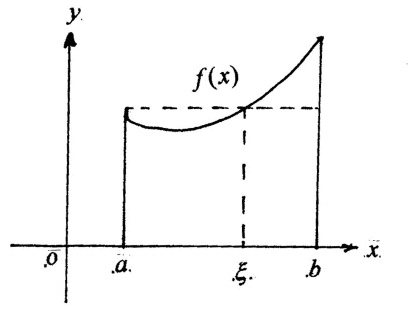
\includegraphics{resources/Geometric_explanation_of_the_mean_value_theorem_for_integration.jpg}
\end{center}

以下为证明:

在不失去一般性的条件下,设对所有的$x$,有$g(x) \geq 0$;因为$\fint$是闭区间上的连续函数,$\fint$取得最大值$M$和最小值$m$.于是得出不等式:

$mg(x) \leq \defFunction{x}g(x) \leq Mg(x)$

对不等式求积分,得出:

$m\definiteIntegral{b}{a}g(x)dx \leq \definiteIntegral{b}{a}\defFunction{x}g(x)dx \leq M\definiteIntegral{b}{a}g(x)dx$

如果$\definiteIntegral{b}{a}g(x)dx = 0$,则$\definiteIntegral{b}{a}\defFunction{x}g(x)dx = 0$.$\xi$可以取$[a,b]$上任意一点.

如果不等于$0$,那么$\definiteIntegral{b}{a}g(x)dx>0$,对不等式变形可得:

$m \leq \cfrac{\definiteIntegral{b}{a}\defFunction{x}g(x)dx}{\definiteIntegral{b}{a}g(x)dx} \leq M$

因为$f(x)$是连续函数,所以上面这玩意是个连续函数,所以必定存在一点$\xi\in[a,b]$,使得

$\defFunction{\xi} = \cfrac{\definiteIntegral{b}{a}\defFunction{x}g(x)dx}{\definiteIntegral{b}{a}g(x)dx}$

($g<0$时也可以按这个步骤推出)
\\\\
推论:拉格朗日中值定理的积分形式

在上式中令$g(x) = 1$,则可得出:

设$\fint : [a,b] \to \mathbf{R}$为一连续函数,则$\exists\xi\in[a,b]$,使得

$\defFunction{\xi} = \cfrac{\definiteIntegral{b}{a}\defFunction{x}dx}{b - a}$

也可以由拉格朗日中值定理推出:

设$F(x)$在$[a,b]$上可导,$\defFunction{x} = F\prime(x)$,则$\exists\xi\in[a,b]$,使

$\defFunction{\xi} = F\prime(\xi) = \cfrac{F(b) - F(a)}{b - a} = \cfrac{\definiteIntegral{b}{a}\defFunction{x}dx}{b - a}$

}%积分第一中值定理结尾

\subsubsection{积分第二中值定理}{

积分第二中值定理与积分第一中值定理相互独立,却又是更精细的积分中值定理.

若$f,g$在$[a,b]$上可积且$f(x)$在$[a,b]$上单调,则存在$[a,b]$上的点$\xi$使

$\definiteIntegral{b}{a}\defFunction{x}dx = \defFunction{a}(\xi - a) + \defFunction{b}(b - \xi)$

进而导出:

$\definiteIntegral{\xi}{a}\defFunction{x}dx -\defFunction{a}(\xi - a) = \defFunction{b}(b - \xi) - \definiteIntegral{b}{\xi}\defFunction{x}dx$

他的几何意义很明显为:能找到$\xi\in[a,b]$,使得红色区域的面积和蓝色区域的面积相加等于阴影区域的面积,即S[\uppercase\expandafter{\romannumeral1}] = S[\uppercase\expandafter{\romannumeral2}]

\begin{center}
  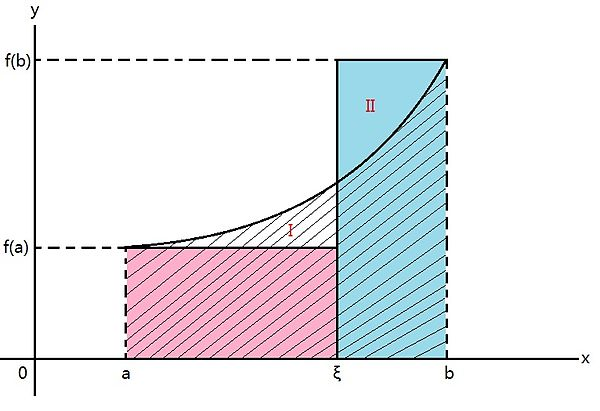
\includegraphics{resources/Geometric_explanation_of_the_second_mean_value_theorem_for_integration.jpg}
\end{center}

}%积分第二中值定理结尾

\subsubsection{定积分求平面函数曲线弧长}{

  $$
    \begin{cases}
      x = \varphi(t) \\
      y = \Phi(t)
    \end{cases}
    \alpha \leq t \leq \beta
    \qquad\qquad\qquad\qquad\qquad\qquad\qquad\qquad\qquad\qquad\qquad\qquad
    \begin{cases}
      x = x \\
      y = \defFunction{x}
    \end{cases}
    \alpha \leq t \leq \beta
  $$

  $S = \definiteIntegral{\beta}{\alpha}\sqrt{\varphi^{\prime 2}(t) + \Phi^{\prime 2}(t)}dt\qquad\qquad\qquad\qquad\qquad\qquad\qquad\qquad\qquad\qquad\qquad S = \definiteIntegral{\beta}{\alpha}\sqrt{1 + y^{\prime 2}}$

  极坐标的情况:

  $$
    \begin{cases}
      x = \rho(\theta)\cos\theta \\
      y = \rho(\theta)\sin\theta
    \end{cases}
  $$

  $S = \definiteIntegral{\beta}{\alpha}\sqrt{\rho^{\prime 2}(\theta) + \rho^2(\theta)d\theta}$\qquad(注意求导符号)
}%定积分求平面函数曲线弧长

}%定积分结尾

\subsection{反常积分}{
通常来说只需要极限存在,则此反常积分收敛.

\subsubsection{无穷限反常积分}{

  有以下几种情况:

  \begin{enumerate}
    \item $\definiteIntegral{+\infty}{a}\defFunction{x}dx = \limNormal{b \to +\infty}\definiteIntegral{b}{a}\defFunction{x}dx$
    \item $\definiteIntegral{b}{-\infty}\defFunction{x}dx = \limNormal{t \to -\infty}\definiteIntegral{b}{t}\defFunction{x}dx$
    \item $\definiteIntegral{+\infty}{-\infty}\defFunction{x}dx = \definiteIntegral{0}{-\infty}\defFunction{x}dx + \definiteIntegral{+\infty}{0}\defFunction{x}dx$
  \end{enumerate}
}%无穷限反常积分结尾


\subsubsection{无界函数反常积分}{

  设b为瑕点:

  \begin{center}
    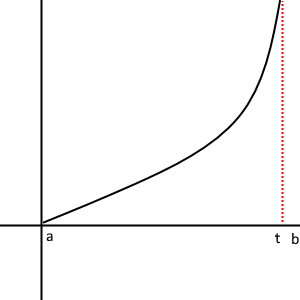
\includegraphics[scale=0.5]{resources/infityFunctionUnormalIntegral.png}
  \end{center}

  $\definiteIntegral{b}{a}\defFunction{x}dx = \limNormal{t \to b^-}\definiteIntegral{t}{a}\defFunction{x}dx$

  或者是设a为瑕点:

  \begin{center}
    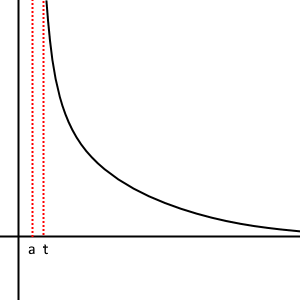
\includegraphics[scale=0.5]{resources/infityFunctionUnormalIntegral2.png}
  \end{center}

  $\definiteIntegral{b}{a}\defFunction{x}dx = \limNormal{t \to a^+}\definiteIntegral{b}{t}\defFunction{x}dx$

  或者以上两者情况合一,设c为瑕点将其拆分:

  \begin{center}
    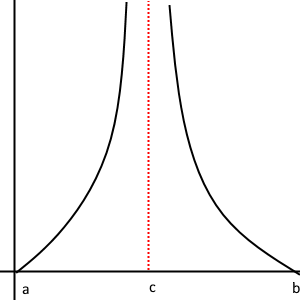
\includegraphics{resources/infityFunctionUnormalIntegral3.png}
  \end{center}

  $\definiteIntegral{b}{a}\defFunction{x}dx = \definiteIntegral{c}{a}\defFunction{x}dx + \definiteIntegral{b}{c}\defFunction{x}dx$

  然后按照上方两个情况分别求解.

  依然可以使用牛-莱公式.

  瑕积分换元需要为单调函数,不论增减性.

}%无界函数反常积分

\subsubsection{gamma函数}{
$\varGamma(s) = \definiteIntegral{+\infty}{0}e^{-x}x^{s-1}dx, (s > 0)$

gamma函数的特点就是:

$\varGamma(s + 1) = s\varGamma(s), \varGamma(1) = 1$

因此:

$\varGamma(n+1) = n!$

}%gamma函数结尾

}%反常积分结尾

\subsection{无穷级数}{

\subsubsection{泰勒公式/泰勒级数/展开}{
泰勒级数表示:当知道某点$x = a$的情况时,就能知道$a$点附近的函数是怎样的.

$x$在$a$点附近,最为粗略的估计就是$\defFunction{x} \approx \defFunction{a}$

然后才是修正项:$\fDerivative{a}(x - a)$,这是斜率乘以距离,最终得到的就是高度.相当于沿切线前进.

还有一项表示弯曲:$\cfrac{1}{2}\fint\doubleDerivative(a)(x - a)^2$,他是斜率的斜率,变化率的变化率.

但后面还有更多项,直接写出通项公式如何?

泰勒级数通项公式:$\defFunction{x} = \upDownSum{\infty}{n = 1}\cfrac{1}{n!}\fint\aLotDerivative{n - 1}(x - a)^{n - 1}$,0阶导指的是原函数,a是x附近的点.

还有泰勒公式:表示的不是一个函数的幂级数形式而是对于某个函数的近似,形式与泰勒级数通项公式类似.

泰勒公式:$\defFunction{x} = \defFunction{a} + \fDerivative{a}(x - a) + \cfrac{1}{2!}\fint\doubleDerivative(a)(x - a)^2 + ... + \cfrac{1}{n!}\fint\aLotDerivative{n}(x - a)^n + R_n(x)$.

$R_n(x)$是余项,表示误差,是$(x - a)^n$的高阶无穷小$O((x - a)^n)$.根据中值定理可得$R_n(x) = \cfrac{1}{(n + 1)!}\fint\aLotDerivative{n + 1}(\xi)(x - a)^{n+1}$,其中$a \leq \xi \leq x$,意思是$\xi$介于$a$和$x$之间.

当泰勒公式在$a = 0$处展开时就称为麦克劳林公式.

麦克劳林公式:当$a = 0, \defFunction{x} = \defFunction{0} + \cfrac{1}{1!}\fDerivative{0}x + \cfrac{1}{2!}\fint\doubleDerivative(0)x^2 + ... + \cfrac{1}{(n + 1)!}\fint\aLotDerivative{n + 1}(\theta x)x^{n+1}$,其中$0 < \theta < 1$

}%泰勒公式/泰勒级数/展开结尾

}%无穷级数结尾

\subsection{微分方程}{
微分方程是一种描述世界的好手段,当描述某个东西随时间的微小变化比起描述这个物体整体的变化更方便的时候就会使用微分方程.

\subsubsection{一阶线性微分方程}{
  形式$\cfrac{dy}{dx} + p(x)y = Q(x)$

  有以下几种情况:
  \begin{enumerate}
    \item $Q(x) = 0\ \to$齐次方程,则$\cfrac{dy}{dx} = -p(x)y\ \to \ \cfrac{dy}{y} = -p(x)dx$,然后两边求积分,从而得出:$y = e^{-\int p(x)dx}e^{\mathConstant_1} = C \cdot e^{-\int p(x)dx}$
    \item {
          $\cfrac{dy}{dx} + p(x)y = Q(x), Q(x) \neq 0$,也就是非齐次方程.设$y = ue^{-\int p(x)dx, u}$是未知量.然后把$y$代入:

          $$
            u\derivative e^{-\int p(x)dx} - ue^{-\int p(x)dx}p(x) + p(x)ue^{-\int p(x)dx} = Q(x)
          $$

          从而推出:
          $$
            u\derivative e^{-\int p(x)dx} = Q(x)
          $$

          因此$u\derivative = Q(x)e^{\int p(x)dx}$,从而推出:
          $$
            u = \int Q(x)e^{\int p(x)dx}dx + \mathConstant
          $$

          将以上带入,得出:$y = e^{-\int p(x)dx}\cdot(\int Q(x)e^{\int p(x)dx}dx + \mathConstant)$\ (通用公式)
          }
  \end{enumerate}

  注:一个非齐次线性微分方程的通解等于对应的齐次微分方程的通解与非齐次微分方程的一个特解之和.

}%一阶线性微分方程结尾

\subsubsection{伯努利方程}{
  $$
    \cfrac{dy}{dx} + p(x)y = Q(x)y^n
  $$

  当$n = 0$时,此式为齐次方程,当$n = 1$,为一阶线性微分方程.

  当$n$即不等于$0$也不等于$1$时,用$y^n$除以两边,得到 :
  $$
    y^{-n}\cfrac{dy}{dx} + p(x)y^{1 - n} = Q(x)
  $$

  设$y^{1 - n} = z$,则 :
  $$
    \cfrac{dz}{dx} = (1 - n)y^{-n}\cfrac{dy}{dx} \to \cfrac{1}{1 - n}\cfrac{dz}{dx} = y^{-n}\cfrac{dy}{dx}
  $$

  代入原方程,则原式等于 :
  $$
    \cfrac{1}{1 - n}\cfrac{dz}{dx} + p(x)z = Q(x)
  $$

  再两侧同乘$\cfrac{dz}{dx}$ :
  $$
    \cfrac{dz}{dx} + (1 - n)p(x)z = (1 - n)Q(x)
  $$

  再套用非齐次线性微分方程的公式,再把$y$求出来就行.
}%伯努利方程结尾

\subsubsection{可降阶高阶微分方程}{
  有以下几种情况:

  \begin{enumerate}
    \item $y^{(n)} = \defFunction{x}$,于是两边不断求积分进行降阶:$y^{n-1} = \int \defFunction{x}dx + \mathConstant$
    \item $y\doubleDerivative = \defFunction{x,y\derivative}$,设$y\derivative = p,y\doubleDerivative = p\derivative$,则$p\derivative = \defFunction{x,p}$.然后再进行回代.
    \item $y\doubleDerivative = \defFunction{y,y\derivative}$,同样的,令$y\derivative = p, y\doubleDerivative = \cfrac{dp}{dx} = \cfrac{dp}{dy}\cdot\cfrac{dy}{dx} = p\cfrac{dp}{dy}$,于是$p\cfrac{dp}{dy} = \defFunction{y,p}$
  \end{enumerate}

}%可降阶高阶微分方程结尾

\subsubsection{常系数齐次线性微分方程}{
  例:$y\doubleDerivative + py\derivative + qy = 0$

  先找出特征方程:$r^2 + pr + q = 0$,即:设$r = p\derivative,r^2 = \doubleDerivative$.

  有以下三种情况:
  \begin{enumerate}
    \item $\Delta = b^2 - 4ac = p^2 - 4q > 0,r_1 = \cfrac{-p + \sqrt{p^2 - 4q}}{2}, r_2 = \cfrac{-p - \sqrt{p^2 - 4q}}{2}$
    \item $\Delta = b^2 - 4ac = p^2 - 4q = 0,r_1 = r_2 = \cfrac{-p}{2}$
    \item {$\Delta = b^2 - 4ac = p^2 - 4q < 0,r_1 = \alpha + \beta_i, r_2 = \alpha - \beta_i$,可扩写成以下三种形式:

          \begin{enumerate}
            \item $y = \mathConstant_1e^{r_1x} + \mathConstant_2e^{r_2x}$($\mathConstant_1,\mathConstant_2$为任意常数)
            \item $y = (\mathConstant_1 + \mathConstant_2)e^{r_1x}$
            \item $y = e^{\alpha x}(\mathConstant_1\cos\beta + \mathConstant_2\sin\beta)$
          \end{enumerate}
          }
  \end{enumerate}

}%常系数其次线性微分方程结尾

\subsubsection{关于运动的微分方程/线性常系数微分方程}{
开门见山,先提出此公式再进行分析.

$m\cfrac{d^2y}{dt^2} + 2r\cfrac{dy}{dt} + ky = 0$

很明显,这是个二阶常系数线性微分方程,二阶指的是它最多求了2次导.线性、这意味着他可以是个抽象的向量,他能被线性代数的方式所表示(见4.1.2-关于抽象向量空间).至于“常系数”,这意味着它的系数都是常数.

先分析这个方程的退化形式.

1、设$m = 0, r = 1/2, \cfrac{dy}{dt} = ay$

很明显:这意味着函数求导后是它自身的倍数,这暗示着原函数是个指数函数.不难猜到:原函数可以为$y = e^{at}$.但这样还不够.仔细想想:如果e的前面有系数,求导后也依然还是原函数的倍数,所以通解应该是$y = ce^{at}$.

2、设 $r = 0, \cfrac{d^2y}{dt^2} = -\omega^2y$,其中$\omega$是$\cfrac{k}{m}$.

这又意味着什么?这意味着:原函数求二次导后是负数倍的他自己,在实数范围内(毕竟一涉及$i$事情就麻烦了起来,不过如果包含虚数的范围倒也是一件合理的事情,设$y=e^{kx},y\doubleDerivative = k^{2}e^{kx}$,如果要使这个二阶导符合条件很明显$k$应该是$i$,而欧拉公式的完整写法是:$e^{ix} = \cos x + i\sin x$)符合这个条件的就这两个函数:$\sin\omega t$和$\cos\omega t$,那么这两个函数就是解集的“基向量/基础解系”,通过这两个函数的线性组合就可以得出所有符合条件的原函数,因此通解写作$y = C\cos\omega t + D\sin\omega t$

3、设$m = 0, r = 0, \cfrac{dy}{dt} = 0$

这更明显,$y = C + Dt$.(y是个函数,表示位置)

那么回到那个方程:这个方程在很多领域都是很常见的.这个方程能表示一切振动.(比如弹簧,钟表,摆动...)通过选择不同的系数,可以建立各种最简洁的基础模型.

那么以弹簧为例来讲解.例子中$t$表示时间(这就是为什么不用x):

实际上,在这种模型中,常有$r = 0$.那么取$ r = 0$的情况.

有牛顿定律:$F = ma$,m就是质量,a则是加速度,也就是二阶导,因此改写成二阶导形式:$F = m\cfrac{d^2y}{dt^2}$(不考虑质量损失)

弹簧是悬空拉着一个小滑块的.y的正方向是向下,他表示弹簧的位移,当y是正的时候,弹簧有向上拉的力,而弹簧的力与$y$成正比,比例则是常数$k$.当y很大的时候弹簧被拉的很长,向上拉的力在往上拉,写作$F = -ky = m\cfrac{d^2y}{dt^2}$其中F表示拉力,负号是因为力的方向与y相反(胡克定理).经过变形得到:$m\cfrac{d^2y}{dt^2} + ky = 0$.非常眼熟.

$r = 0$,$r$表示的是阻力,可以是空气阻力也可以是磁力等等,他就是没法制作永动机的原因,不过现在是假想环境,所以设他为0,那么弹簧就会是一根永不停息的、上下振动的弹簧.就如同上面分析的结果,他沿着{\bfseries 正弦和余弦}振动.而常数$C$与$D$则取决于初始状态.

回想一下,$-ky = m\cfrac{d^2y}{dt^2}$,将两边同除以$m$,负号移走,于是得到$\omega^2$而$\omega^2 = \cfrac{k}{m}$.

这种情况很简单,只有$\sin , \cos$.接下来,来一点阻力.

$my\doubleDerivative + 2ry\derivative + ky = 0$

现在,对于任意$m,r,k$.想要求解此方程,很棒的是指数函数可以求出正确答案.

核心思想是尝试指数函数$y = e^{\lambda t}$,$\lambda$指的是特征函数.(用$\lambda$而不用$C$的原因可以看4.1.1-什么是线性变换.)将这个代入方程,并求出合适的$\lambda$.何不先从常数项开始?

很容易看出常数项是$ke^{\lambda t}$

而一阶导呢?有$2r$乘以$y = e^{\lambda t}$的导数,只需要将导数代入方程.

一阶项是$2r\lambda e^{\lambda t}$

到二阶导,同理.

二阶项就是$m\lambda^2e^{\lambda t}$

写出完整的形态:$m\lambda^2e^{\lambda t} + 2r\lambda e^{\lambda t} + ke^{\lambda t} = 0$

消掉公因式$e^{\lambda t}$,他显然不是0,可以消掉.结果就是$m\lambda^2 + \lambda + k= 0$

这个方程只不过是个普通的二次方程,随随便便就能解出来.二次方程理应有两个解.因此$e^{\lambda_1 t}$和$e^{\lambda_2 t}$都是方程的解

回忆一下公式,$\lambda = \cfrac{-r \pm \sqrt{r^2 - km}}{m}$

引入一些数字,$1y\doubleDerivative + 6y\derivative + 8y = 0$.计算$\lambda$

$\lambda^2 + 6\lambda + 8 = 0$

$\lambda_1 = -2, \lambda_2 = -4$

解是多少呢?$y(t) = Ce^{-2t} + De^{-4t}$

两个$\lambda$都在指数中,然后得解

注意:$\lambda$可能解出复数,可以照样用,但也可以写成另一种形式——利用欧拉公式的美妙性质.

$e^{it} = \cos t + i\sin t$

(欧拉第二天意识到$-i$也有公式)

$e^{-it} = \cos t -i\sin t$

直接跳到结果:

$e^{(x \pm ki)t} = e^{xt}\cdot(\cos(t\cdot n) \pm i\sin(t\cdot n))$

另外,当两个$\lambda$相同(出现重根)的时候,方程的解一个是$e^{\lambda t}$另一个是$te^{\lambda t}$,经过验算会发现最后消掉了一部分,得到的是正常的结果.

所以结论就是:线性常系数微分方程只要通过$e^{\lambda t}$就能解决.
}%关于运动的微分方程结尾

\subsubsection{关于增长的微分方程/非线性微分方程/偏微分方程剧透}{
  从线性的开始.

  最简单的:$\cfrac{dy}{dt} = cy$, 给予了初始条件$y(0)$

  即增长率与自身成正比.很明显的这是呈指数形式的增长,解应该是$y(t) = y(0)e^{ct}$

  看下一个方程,依然是线性的:$\cfrac{dy}{dt} = cy + s$,$s$表示source,可以用银行存钱来描述:前一项是每天的利息,后一项的每天存入的金额.
  这就是右侧带有常数项的线性微分方程了.事实上甚至能拿现有的知识来解决它:$\cfrac{dy}{dt} = cy + s = c(y + \cfrac{s}{c}) = \cfrac{d(y + \cfrac{s}{c})}{dt}$, 其中$\cfrac{s}{c}$是常数,所以可以任意加减而不影响求导结果.随后观察整体,会发现与第一个例子几乎相同,唯一不同的就是多了个$\cfrac{s}{c}$函数依然以增长率c增长.从0处的y值加上$\cfrac{s}{c}$开始.

  所以,结论是:$y(t) + \cfrac{s}{c} = (y(0) + \cfrac{s}{c})e^{ct}$.这就是该微分方程的快速版解答了.将常数丢到右边,就是一个标准的形式.

  所以线性方程(不只是线性微分方程)的解$y(t) = y_{particular}(t) + y_{another\ solution\ with\ a\ right\ side\ 0}(t)$.用人话说就是:线性方程的解总是自身的某个特解加上另一个右侧等于0的方程的解.

  也就是说如果要求$\cfrac{dy}{dt} = cy + s$的解,那么首先求一个特解(也就是任一个满足方程的函数),能找到的最简单的函数就是常函数.想要常数满足方程,常熟的常数必然为0,而且c乘以此常数加s也应该为0.也就是$cy + s = 0,\ cy = -s, \ y = -\cfrac{s}{y}$.这就是一个特解了.

  那么“一个右侧为0的方程的解”是什么意思?将s擦去,使得$\cfrac{dy}{dt} = cy$,保留含有y的,去掉常数项,使得右侧为0.也就是$y\derivative - cy = 0$.书本上喜欢称之为:齐次方程.也就是第一个例子.

  那么齐次方程的解是什么呢?$\cfrac{dy}{dt} = cy$的解含有$e^{ct}$以及任意常数$A$,也就是$Ae^{ct}$,任意$Ae^{ct}$都能满足这个简单的方程.

  所以整个方程的解就是$-\cfrac{s}{c} + Ae^{ct}$A是任意常数.不过当然,如果有初始条件就能特定一个.只需要设$t = 0$,就能解出$A$,在这里$A = y(0) + \cfrac{s}{c}$.在上面也算出来了.

  不过线性的已经没啥意思了,来点线性的.非线性的微分方程很有趣,也可以表示很多东西,比如:人口的增长.

  关于人口增长函数$P(t)$,用什么微分方程描述比较合理?

  $\cfrac{dP}{dt} = cP - sP^2$.其中c表示增长率.同样的,有出生也会有死亡,所以需要一个减速项,因为人口增长不可能这么快.也就是s.这在一定程度上反映了人口之间的相互作用.(事实上这种公式在其他领域也有很多用途)

  在这个公式中$p^2$表示人口之间的相互拥挤造成的影响,因此s是个很小的数,比如十亿分之一.

  下面要解这个方程了.

  不过对于非线性方程,目前(正在阅读的你,或者是我自己复习?)暂时没有现成的工具,需要更多的微积分知识.但是只要方法正确,就能解出来的.

  先展示解吧:首先,如果一开始一个人都没有,那么就始终为0.$P = 0$,常数解,很无趣.还有一种情况,很重要的情况,这种情况下导数也为0.

  假设导数为0,将会得到一个特殊的特解,他不会变化.也就是当导数为0时,那么$cP = sP^2$.可以约掉一个P,也就是$P = \cfrac{C}{S}$.此时,增长和减少将会相互抵消,成为无法逾越的上限.

  那么来看看真实情况下的解,不过为何不先看看图呢?:

  \begin{center}
    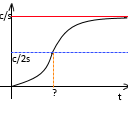
\includegraphics{resources/nonLinearDifferencialEquation_HumanGrow.png}
  \end{center}

  其中$\cfrac{c}{s}$称为稳态,到了这里就会保持稳定,不会改变了.不过其实到不了哪里,只会一直接近而已.这就是这个式子所代表的人口曲线了.

  那么就是解方程的环节了.有很多方法,先试试一个好使的:尝试$y = \cfrac{1}{P}$.然后尝试把整个方程写成y的形式.这是解这个方程的技巧,而解非线性方程常常需要一些技巧.

  看看这个方程长啥样子:$\cfrac{dy}{dt} = -\cfrac{\cfrac{dP}{dt}}{P^2}$而$\cfrac{dP}{dt}$是已知的,所以将他代进来,得到$-\cfrac{cP - sP^2}{P^2}$.将负号写进去,得到一个s:$s - \cfrac{c}{P}$.查看前面的推导能发现:$\cfrac{1}{p} = y$.所以得到$s - cy$.于是$\cfrac{dy}{dt}$变成了线性的,它还含有资源项s,而增长率项还含有一个-c.也许仔细想想为什么

  那么写出y的解:$y(t) - \cfrac{s}{c} = (y(0) - \cfrac{s}{c})e^{-ct}$这就是y的解.$y = \cfrac{1}{P}$,接下来就是要回代了:

  $\cfrac{1}{P(t)} - \cfrac{s}{c} = (\cfrac{1}{P(0)} - \cfrac{s}{c})e^{-ct}$,接下来的一堆化简就不写了.

  这种模型称为logistic方程(只是为了提一下)

  接下来再来一个有意思的方程:捕食者与猎物的方程:

  这里有两个未知数:猎物——记作$v$,捕食者——记作$u$,表示的都是两者的总数.如果猎物不够,捕食者就会减少.捕食者减少,猎物就会增加.因此这里有正的$u \cdot v$

  这是公式:

  前面有个$-cu$,表示没有食物的情况,捕食者将会慢慢灭绝.

  但如果猎物存在,那么资源项就会正比于$uv$.

  所以$\cfrac{du}{dt} = -cu + suv$

  那么$\cfrac{dv}{dt}$呢?情况大不相同.他们被捕食,因此有$-Suv$,同时也有正的增长率$Cv$

  那么这就是一个模型了.剧透一下:这玩意叫偏微分方程(Partical Differential Equation),简称PDE,他比常微分方程(Ordinary Differential Equation, ODE)包含了更多的信息.也更难解.

}%关于增长的微分方程结尾

}%微分方程结尾

}%微积分结尾

\section{多元微积分}{
注:如果忘了什么是偏导数就去上一章回顾.
%# TODO: 重新学一遍

\subsection{多元函数的极值与最值}{

  \subsubsection{多元函数的极值}{
    \begin{itemize}
      \item {
            极值存在的必要条件 :

            如果$z = \defFunction{x,y}$有偏导且在$(x_0,y_0)$存在极值,则$f\derivative_x(x_0,y_0) = 0,f\derivative_y(x_0,y_0) = 0$

            驻点此时指偏导等于0的点,即$f\derivative_x = f\derivative_y = 0$(需要同时成立).

            有偏导数的函数极值点必是驻点.但是函数的驻点不一定是极值点.
            }
      \item {
            极值存在的充分条件 :

            依然是拿$z = \defFunction{x,y}$举例:

            首先求出驻点$(x_0,y_0)$,$A = f\doubleDerivative_{xx},B = f\doubleDerivative_{xy}(x_0,y_0),C = f\doubleDerivative_{yy}(x_0,y_0)$

            \begin{itemize}
              \item {当$AC-B^2 > 0$时,存在极值点.其中 :
                    \begin{itemize}
                      \item $A < 0$,极值点为极大值.
                      \item $A > 0$,极值点为极小值.
                    \end{itemize}
                    }
              \item 当$AC - B^2 > 0$时,无极值.
              \item 当$AC - B^2 = 0$时,无法判断.
            \end{itemize}
            }
    \end{itemize}
  }%多元函数的极值结尾

  \subsubsection{多元函数的最值}{
    多元函数的最值一般出现在三种情况中 :

    \begin{enumerate}
      \item 驻点
      \item 偏导不存在的点
      \item 端点
    \end{enumerate}
  }%多元函数的最值结尾

  \subsubsection{条件极值与拉格朗日乘数法}{
    设目标函数为$z = \defFunction{x,y}$,条件为$\varphi(x,y) = 0$

    假设$y$也是$x$的函数$\psi$,则 :

    $$
      z = \defFunction{x,\psi(x)}
    $$

    如果对$x$的导数存在且有极值,那么求导应该为$0$,因此对$z$求导 :
    $$
      \cfrac{dz}{dx} = \partialDerivativeFrac{f}{x} + \partialDerivativeFrac{f}{y}\cdot\cfrac{dy}{dx}
    $$

    那么 :
    $$
      \directionDerivative{z}{x}{x = x_0} = f\derivative_x(x_0,y_0) + f\derivative_y(x_0,y_0)\directionDerivative{y}{x}{x = x_0} = 0
    $$

    由此结论,把$y$看作$x$的隐函数,则由隐函数存在定理 : $\cfrac{dy}{dx} = -\cfrac{\varphi\derivative_x(x,y)}{\varphi\derivative_y(x,y)}$

    将其代入,从而得到 :
    $$
      f\derivative_x(x_0,y_0) - f\derivative_y(x_0,y_0)\cfrac{\varphi\derivative_x(x,y)}{\varphi\derivative_y(x,y)} = 0
    $$

    设后一项中的$-\cfrac{f\derivative_y(x_0,y_0)}{\varphi\derivative_y(x_0,y_0)} = \lambda$

    代入替换,得 :
    $$
      f\derivative_x + \lambda\varphi\derivative_x = 0
    $$

    并且对$\lambda$作变形 :
    $$
      f\derivative_y(x_0,y_0) - \cfrac{f\derivative_y(x_0,y_0)}{\varphi\derivative_y(x_0,y_0)}\varphi\derivative_y(x_0,y_0) = f\derivative_y + \lambda\varphi\derivative_y = 0
    $$

    联立方程组 :
    $$
      \begin{cases}
        f\derivative_x + \lambda\varphi\derivative_x = 0 \\
        f\derivative_y + \lambda\varphi\derivative_y = 0 \\
        \varphi(x_0,y_0) = 0
      \end{cases}
    $$

    作辅助函数$L(x,y) = \defFunction{x,y} + \lambda\varphi(x,y)$

    $$
      \begin{cases}
        L\derivative_x = 0 \\
        L\derivative_y = 0
      \end{cases}
      \mbox{即 : }
      \begin{cases}
        f\derivative_x + \lambda\varphi\derivative_x = 0 \\
        f\derivative_y + \lambda\varphi\derivative_y = 0 \\
        \varphi(x,y) = 0
      \end{cases}
    $$

    当有两个以上的约束条件时 :

    $u = \defFunction{x,y,z,t},\varphi(x,y,z,t) = 0,\psi(x,y,z,t) = 0$

    $L = \defFunction{x,y,z,t} + \lambda\varphi(x,y,z,t) + \mu\psi(x,y,z,t)$

    $$
      \begin{cases}
        L\derivative_x = 0   \\
        L\derivative_y = 0   \\
        L\derivative_z = 0   \\
        L\derivative_t = 0   \\
        \varphi(x,y,z,t) = 0 \\
        \psi(x,y,z,t) = 0
      \end{cases}
    $$
  }%条件极值与拉格朗日乘数法结尾

}%多元函数的极值与最值结尾

\subsection{隐函数}{

  \subsubsection{隐函数存在定理/隐函数定理(二元)}{
    %# TODO 填坑
  }%隐函数存在定理/隐函数定理(二元)结尾

}%隐函数结尾

\subsection{重积分}{

  \subsubsection{二重积分}{
    定义 : $\limNormal{\lambda \to 0}\upDownSum{n}{i = 1}\Delta\sigma_i\defFunction{\xi_i,\eta_i} = \doubleIntegralOnZone{D}\defFunction{x,y}d\sigma$

    解释 : $\defFunction{x,y}$是区域$D$上的有界函数,将区域$D$任意分成$n$个区域$\Delta\sigma_1\dots\Delta\sigma_n$,在每个$\Delta\sigma_i$上任取一点,$(\xi_i,\varUpsilon_i)\cdot\Delta\sigma_i$,当$\lambda \to 0$时,如果上述极限存在,则称为$f(x,y)$的二重积分.其中$d\sigma$称为面积元素,可写作$dxdy$

    设被积函数$\defFunction{x,y}$,从几何上来说 :
    \begin{itemize}
      \item 当$\defFunction{x,y} \geq 0$时,二重积分结果为体积.
      \item 当$\defFunction{x,y} < 0$时,二重积分结果为体积的相反数.
      \item 当$\defFunction{x,y}$有正有负时,二重积分结果为$XOY$平面上半部分的体积减去下半部分的体积.
    \end{itemize}
  }%二重积分结尾

  \subsubsection{二重积分的性质}{
    \begin{itemize}
      \item $\doubleIntegralOnZone{D}\left[\alpha\defFunction{x,y} + \beta g(x,y)\right]d\sigma = \alpha\doubleIntegralOnZone{D}\defFunction{x,y}d\sigma + \beta\doubleIntegralOnZone{D}g(x,y)d\sigma$
      \item $D$分为$D_1,D_2$,$\doubleIntegralOnZone{D}\defFunction{x,y}d\sigma = \doubleIntegralOnZone{D_1}\defFunction{x,y}d\sigma + \doubleIntegralOnZone{D_2}\defFunction{x,y}d\sigma$
      \item $f(x,y) = 1,\doubleIntegralOnZone{D}f(x,y)d\sigma = \sigma$
      \item $\defFunction{x,y} \leq g(x,y), \doubleIntegralOnZone{D}\defFunction{x,y}d\sigma \leq \doubleIntegralOnZone{D}g(x,y)d\sigma$
      \item $\left|\doubleIntegralOnZone{D}\defFunction{x,y}d\sigma\right| \leq \doubleIntegralOnZone{D}\left|\defFunction{x,y}\right|d\sigma$
      \item $M,m$分别是函数的最高和最低点,$m\sigma \leq \doubleIntegralOnZone{D}\defFunction{x,y} \leq M\sigma$
      \item $m \leq \cfrac{\doubleIntegralOnZone{D}\defFunction{x,y}d\sigma}{\sigma} \leq M$,即 : $\defFunction{\xi,\eta} = \cfrac{1}{\sigma}\doubleIntegralOnZone{D}\defFunction{x,y}d\sigma$
    \end{itemize}
  }%二重积分的性质结尾

  \subsubsection{直角坐标系下的二重积分计算}{
    \begin{center}
      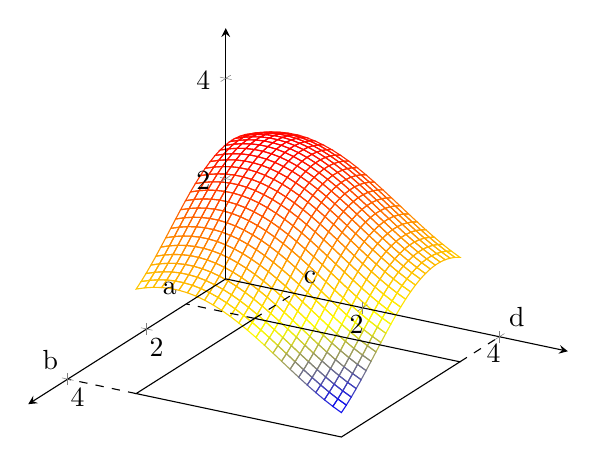
\begin{tikzpicture}
        \begin{axis}[view = {120}{30},axis lines = center,axis on top,xmin = 0,xmax =5,ymin = 0,ymax = 5,zmin = 0,zmax = 5]
          \addplot3[domain=1:4,y domain=1:4,mesh]{2 + sin(deg(x)) + sin(deg(y))};
          \addplot3[color = black] coordinates {(1,1,0)(1,4,0)(4,4,0)(4,1,0)(1,1,0)};
          \addplot3[dashed] coordinates {(1,1,0)(1,0,0)} [above left] node{a};
          \addplot3[dashed] coordinates {(4,1,0)(4,0,0)} [above left] node{b};
          \addplot3[dashed] coordinates {(1,1,0)(0,1,0)} [above right] node{c};
          \addplot3[dashed] coordinates {(1,4,0)(0,4,0)} [above right] node{d};
        \end{axis}

      \end{tikzpicture}
    \end{center}

    思路是将立体对象切成一个个面再进行积分,如下 :

    \begin{center}
      \begin{tikzpicture}
        \draw [->] (0,0) -- (5,0);
        \draw [->] (0,0) -- (0,5);
        \draw (1,3)..controls(2,4) and (3,4)..(4,3);
        \draw (1,0) -- (1,3);
        \draw (4,0) -- (4,3);
        \node (funcZ) at (2.5,4.3){$z = \defFunction{x,y}$};
        \node (point1) at (1,-0.3){$\varphi_1(x)$};
        \node (point1) at (4,-0.3){$\varphi_2(x)$};
        \node (ZAxis) at (5.3,0){Y};
        \node (YAxis) at (0,5.3){Z};
      \end{tikzpicture}
    \end{center}

    此图像的面积$S = \definiteIntegral{\varphi_2(x)}{\varphi_1(x)}\defFunction{x,y}dy$

    再对面积进行积分 : $V = \definiteIntegral{b}{a}\definiteIntegral{\varphi_2(x)}{\varphi_1(x)}\defFunction{x,y}dydx = \definiteIntegral{b}{a}dx\definiteIntegral{\varphi_2(x)}{\varphi_1(x)}\defFunction{x,y}dy = \definiteIntegral{d}{c}\definiteIntegral{\phi_2(y)}{\phi_2(y)}\defFunction{x,y}dxdy$

    在直角坐标系下有两种积分顺序:
    \begin{itemize}
      \item $X$型 : 内层积分时上方函数是上限,下方函数是下限,即:$\definiteIntegral{xx}{xx}\definiteIntegral{\mbox{上}}{\mbox{下}}\defFunction{x,y}dydx$
      \item $Y$型 : 内层积分时左侧函数是下限,右侧函数是上限,即:$\definiteIntegral{xx}{xx}\definiteIntegral{\mbox{左}}{\mbox{右}}\defFunction{x,y}dxdy$
    \end{itemize}
  }%直角坐标系下的二重积分的计算结尾

  \subsubsection{直角坐标系下二重积分的特殊情况}{
    有两种特殊情况可以简化二重积分的运算 :

    \begin{enumerate}
      \item {
            积分区域为长方形 :
            \begin{center}
              \begin{tikzpicture}
                \draw (1,1) rectangle (4,3);
                \node (a) at (2.5,0){a};
                \node (b) at (2.5,4){b};
                \node (c) at (0,2){c};
                \node (d) at (5,2){d};
                \draw[dashed] (a) -- (b);
                \draw[dashed] (c) -- (d);
              \end{tikzpicture}
            \end{center}

            则$\definiteIntegral{b}{a}dx\definiteIntegral{d}{c}\defFunction{x,y}dy = \definiteIntegral{d}{c}dy\definiteIntegral{b}{a}\defFunction{x,y}dx$
            }
      \item {
            在情况 1 下,如果$\defFunction{d}{c} = f_1(x) \cdot f_2(y)$,则 :

            $$
              \definiteIntegral{b}{a}dx\definiteIntegral{d}{c} f_1(x) \cdot f_2(y)dy = \definiteIntegral{b}{a}f_1(x)dx\definiteIntegral{d}{c}f_2(y)dy = \definiteIntegral{b}{a}f_1(x)dx \cdot \definiteIntegral{d}{c}f_2(y)dy
            $$
            }
    \end{enumerate}

  }%直角坐标系下二重积分的特殊情况结尾

  \subsubsection{极坐标下的二重积分计算}{
    \begin{center}
      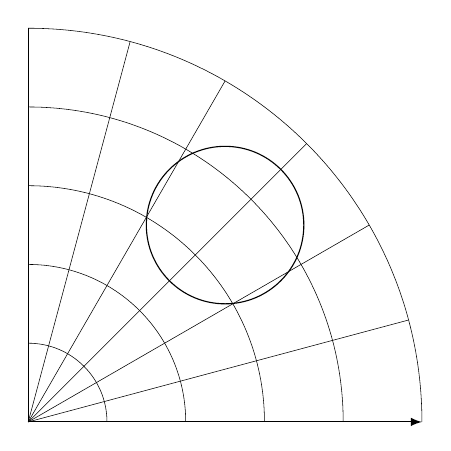
\begin{tikzpicture}
        \draw (0,0) -- (0,5);
        \draw [-latex] (0,0) -- (5,0);
        \draw (2.5,2.5) circle (1);
        \foreach \i in {1,...,5}{
            \draw[line width = 0.2pt] (\i,0) arc (0:90:\i);
          }
        \foreach \j in {1,...,6}{
            \draw[line width = 0.2pt] (0,0) -- (\j * 15:5);
          }
      \end{tikzpicture}
      \qquad\qquad
      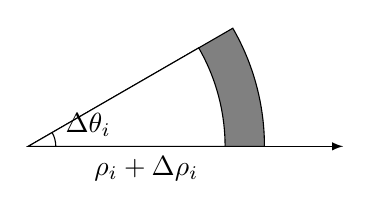
\begin{tikzpicture}
        \filldraw[fill = gray,draw = black] (0,0) -- (3,0) arc (0:30:3) -- cycle;
        \filldraw[fill = white,draw = black] (0,0) -- (2.5,0) arc (0:30:2.5) -- cycle;
        \draw[-latex] (0,0) -- (1.5,0) node[below]{$\rho_i + \Delta\rho_i$} -- (4,0);
        \draw (0.35,0) node[above right]{$\Delta\theta_i$} arc (0:30:0.35);
      \end{tikzpicture}
    \end{center}

    公式的定义为 :
    $$
      \limNormal{\lambda \to 0}\upDownSum{n}{i = 1}\defFunction{\xi_i,\eta_i}\Delta\sigma_i = \limNormal{\lambda \to 0}\upDownSum{n}{i = 1}\defFunction{\bar{\rho_i}\cos\bar{\theta_i}, \bar{\rho_i}\sin\bar{\theta_i}}\cdot\bar{\rho_i}\Delta\rho_i\Delta\theta_i
    $$

    简而言之,将直角坐标系下的二重积分转换为极坐标下的二重积分的公式为 :
    $$
      \doubleIntegralOnZone{D}\defFunction{x,y}d\sigma = \doubleIntegralOnZone{D}\defFunction{\rho\cos\theta,\rho\sin\theta}\rho d\rho d\theta
    $$

    注意 :
    \begin{itemize}
      \item {
            后面多出来了的一个$\rho$要记得加上,这个$\rho$并不是凭空冒出来的,它来自面积元素$d\sigma$ :
            $$
              \Delta\sigma_i = \cfrac{1}{2}(\rho_i + \Delta\rho_i)^2\Delta\theta_i - \cfrac{1}{2}\rho_i^2\Delta\theta_i = \cfrac{\rho_i + (\rho_i + \Delta\rho_i)}{2}\Delta\rho_i - \Delta\theta_i = \bar{\rho_i}\cdot\Delta\rho_i\cdot\Delta\theta_i
            $$
            }
      \item {
            极坐标的积分顺序不能互换
            }
      \item{
            何时使用极坐标 :
            \begin{enumerate}
              \item 积分区域为圆,圆环,扇形
              \item 被积表达式为$x^2 + y^2,\cfrac{x}{y},\cfrac{y}{x}$
            \end{enumerate}
            }
    \end{itemize}

  }%极坐标下的二重积分计算

  \subsubsection{极坐标下的特殊情况}{
    \begin{itemize}
      \item $-x^2 -y^2 = -(\rho^2\cos^2\theta + \rho^2\sin^2\theta) = \rho^2$
      \item $\cfrac{x}{y} = \tan\theta$
      \item $\cfrac{y}{x} = \cot\theta$
    \end{itemize}
  }%极坐标下的特殊情况结尾

  \subsubsection{二重积分换元法}{
    设$\defFunction{x,y}$在$B$区域连续,$x = x(u,v),y = y(u,v)$,且$x,y$积分区域为$D$,用$u,v$换元后为$D\derivative$\\

    当 :
    \begin{enumerate}
      \item $x(u,v),y(u,v)$有一阶连续偏导.
      \item {
            $
              J(u,v)
              =
              \partialDerivativeFrac{(x,y)}{(u,v)} = \begin{bmatrix}
                \partialDerivativeFrac{x}{u} & \partialDerivativeFrac{x}{v} \\
                \partialDerivativeFrac{y}{u} & \partialDerivativeFrac{y}{v}
              \end{bmatrix}
            $
            }
      \item $\absoluteValue{J(u,v)} \neq 0$(不全为0,如果指事字一个点或一条线上为0也成立)
      \item $D\derivative$到$D$点是一一对应的
    \end{enumerate}

    此时 :
    $$
      \doubleIntegralOnZone{D}\defFunction{x,y}dxdy = \doubleIntegralOnZone{D\derivative}\defFunction{x(u,v),y(u,v)}\doubleAbsoluteValue{J(u,v)}dudv
    $$

    从几何直观上看 :
    \begin{center}
      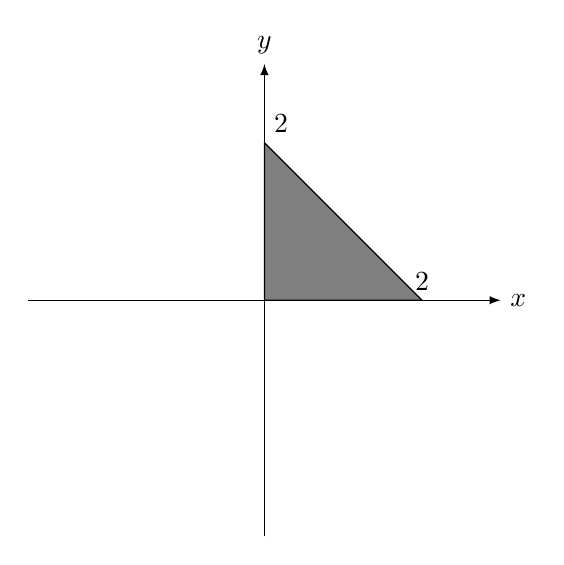
\begin{tikzpicture}
        \draw[-latex] (0,-3) -- (0,3) node[above]{$y$};
        \draw[-latex] (-3,0) -- (3,0) node[right]{$x$};
        \filldraw[fill = gray,draw = black] (0,0) -- (2,0) node[above]{2} -- (0,2) node[above right]{2} -- cycle;
      \end{tikzpicture}
      变成了 :
      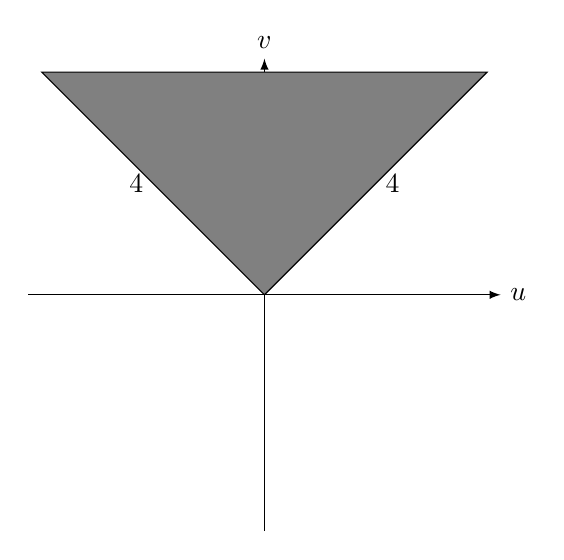
\begin{tikzpicture}
        \draw[-latex] (0,-3) -- (0,3) node[above]{$v$};
        \draw[-latex] (-3,0) -- (3,0) node[right]{$u$};
        \filldraw[fill = gray,draw = black] (0,0) -- node[right]{4}({2*sqrt(2)},{2*sqrt(2)}) -- ({-2*sqrt(2)},{2*sqrt(2)}) -- node[left]{4}cycle;
      \end{tikzpicture}
    \end{center}

    其中$\doubleAbsoluteValue{J(u,v)} = \cfrac{1}{2}$,因此缩放了两倍.\\

    一般来说在以下情况下会使用换元:
    \begin{itemize}
      \item 被积函数不好积
      \item 积分区域不好表示
    \end{itemize}
  }%二重积分换元法结尾

  \subsubsection{三重积分}{
    设$v = \defFunction{x,y,z}$,从空间中任取一点$\Delta V_i : \defFunction{\xi_i,\eta_i,\zeta_i}$

    定义为 :
    $$
      \limNormal{\lambda \to 0}\upDownSum{n}{i = 0}\defFunction{\xi_i,\eta_i,\zeta_i}\Delta V_i = \tripleIntegralOnZone{\Omega}\defFunction{x,y,z}dv = \tripleIntegralOnZone{\Omega}\defFunction{x,y,z}dxdydz
    $$

    $\Omega$表示积分空间区域.

    与二重积分类似,具体积分思路为 :
    \begin{center}
      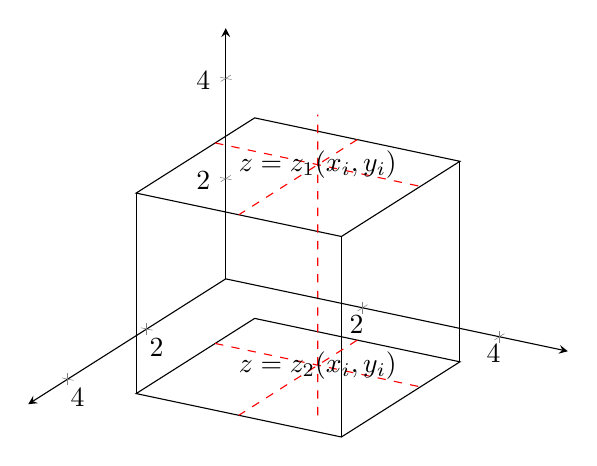
\begin{tikzpicture}
        \begin{axis}[view = {120}{30},axis lines = center,axis on top,xmin = 0,xmax =5,ymin = 0,ymax = 5,zmin = 0,zmax = 5]
          \addplot3[color = black] coordinates {(1,1,0)(4,1,0)(4,4,0)(1,4,0)(1,1,0)};
          \addplot3[color = black] coordinates {(1,1,4)(4,1,4)(4,4,4)(1,4,4)(1,1,4)};
          \addplot3[color = black] table {
              1 1 0 a
              1 1 4 b

              4 1 0
              4 1 4

              4 4 0
              4 4 4

              1 4 0
              1 4 4
            };

          \addplot3[color = red,style = dashed] table {
              2 2.5 -1
              2 2.5 5

              1 2.5 0
              4 2.5 0

              2 1 0
              2 4 0

              1 2.5 4
              4 2.5 4

              2 1 4
              2 4 4
            };

          \draw (axis direction cs:2,2.5,5) node {$z = z_1(x_i,y_i)$};
          \draw (axis direction cs:2,2.5,1) node {$z = z_2(x_i,y_i)$};
        \end{axis}
      \end{tikzpicture}
      $\doubleIntegralOnZone{D(x,y)}\left[\definiteIntegral{z_2(x,y)}{z_1(x,y)}\defFunction{x,y,z}dz\right]dxdy$
    \end{center}

    值得注意的是在二重积分情况下的特殊情况(5.3.4)在三重积分下也适用.
  }%三重积分结尾

  \subsubsection{三重积分(柱面坐标)}{
    由于柱面坐标只是单纯的加了个$z$轴,因此只是单纯的在外面套了一层对$z$轴的积分而已.

    即 : $dv = \rho d\rho d\theta dz$
  }%三重积分(柱面坐标结尾)

  \subsubsection{三重积分(球面坐标)}{
    公式为 :
    $$
      dv = dxdydz = r^2\sin\varphi drd\varphi d\theta
    $$

    多出来的$r^2\sin\varphi$也可以由雅可比行列式推出.
  }%三重积分(球面坐标)结尾

  \subsubsection{重积分应用(求曲面面积)}{
    设$z = \defFunction{x,y}$;将曲面划分称一个个长为$a$宽为$b$�����小方格:

    图示如下 :
    \begin{center}
      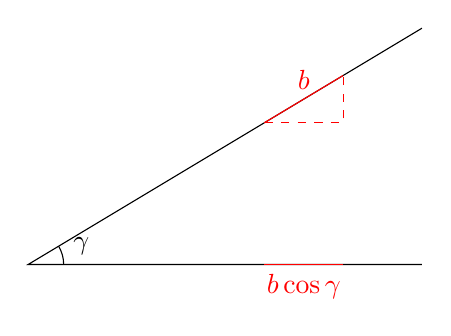
\begin{tikzpicture}
        \draw[color = black] (5,0) -- (0,0) -- (5,3);
        \draw[color = black] (0.45,0) node[above right]{$\gamma$} arc (0 : {deg(0.54)} : 0.45);
        \draw[color = red] (3,0) -- node[below]{$b\cos\gamma$} (4,0);
        \draw[color = red] (3,1.8) -- node[above]{$b$} (4,2.4);
        \draw[color = red,dashed] (3,1.8) -- (4,1.8) -- (4,2.4);
      \end{tikzpicture}
    \end{center}

    设投影后的区域为$d\sigma$,投影前为$dA$.投影后长边的长度$a$不变,因此$dA = \cfrac{d\sigma}{\cos\gamma}$

    其中$\cos\gamma = \cfrac{1}{\sqrt{1 + (f\derivative_x)^2 + (f\derivative_y)^2}}$

    所以$dA = \sqrt{1 + (f\derivative_x)^2 + (f\derivative_y)^2}d\sigma$,即 :

    $$
      A = \doubleIntegralOnZone{D}\sqrt{1 + (f\derivative_x)^2 + (f\derivative_y)^2}d\sigma
    $$
  }%重积分应用(求曲面面积)结尾

  %# TODO 重积分应用(求质心,转动惯量,引力)

}%重积分结尾

\subsection{曲线积分与曲面积分}{
  在数学中,曲线积分或路径积分(或contour integral[留数定理])是积分的一种.积分函数的取值沿的不是区间,而是特定的曲线,称为积分路径.曲线积分有很多种类,当积分路径为闭合曲线时,称为环路积分或围道积分.

  在曲线积分中,被积的函数可以是标量函数或向量函数.当被积函数是标量函数时,积分的值是积分路径各点上的函数值乘上该点切向量的长度.在被积分函数是向量函数时,积分值是积分向量函数与曲线切向量的内积.在函数是标量函数的情形下,可以把切向量的绝对值(长度)看成此曲线把该点附近定义域的极小区间,在到达域内拉长了切向量绝对值的长度,这也是曲线积分与一般区间上的积分的主要不同点.

  \subsubsection{第一类曲线积分(对弧长的曲线积分)}{
    设曲线的密度为$M(x,y)$,求质量$m$:

    \begin{center}
      \begin{tikzpicture}
        \draw[-latex] (0,0) -- (5,0);
        \draw[-latex] (0,0) -- (0,5);

        \draw (1,1) node[left]{$A$} ..  controls (2,1) and (3,2) .. (4,4) node[right]{$B$};
        \draw (2.5,2) rectangle (3.5,2.5);
        \draw[-latex] (3.5,2.25) -- node[above]{放大} (5.5,2.25);
        \draw (5.7,1.3) node[left]{$M_i - 1$} .. controls (6,1) and (7,2) .. node[below right]{$M(\xi_i,\eta_i)$} (7,3) node[right]{$M_i$};
      \end{tikzpicture}
    \end{center}

    第一类曲线积分的定义为 :
    $$
      \limNormal{\lambda \to 0}\upDownSum{n}{i = 1}M(\xi_i,\eta_i)\Delta S_i = m = \pathIntegral{L}\defFunction{x,y}ds
    $$

    其中$ds$称为曲线元素,也有三维的形式$\pathIntegral{L}\defFunction{x,y,z}ds$.

    第一类曲线积分有以下运算性质 :
    \begin{itemize}
      \item $\pathIntegral{L_1 + L_2}\defFunction{x,y}ds = \pathIntegral{L_1}\defFunction{x,y}ds + \pathIntegral{L_2}\defFunction{x,y}ds$
      \item $\pathIntegral{L}(\alpha\defFunction{x,y} + \beta g(x,y))ds = \alpha\pathIntegral{L}\defFunction{x,y}ds + \beta\pathIntegral{L}g(x,y)ds$
      \item $\pathIntegral{L}\defFunction{x,y}ds = \pathIntegral{L_1}\defFunction{x,y}ds + \pathIntegral{L_2}\defFunction{x,y}ds \qquad (L = L_1 + L_2)$
      \item $\defFunction{x,y} \leq g(x,y),\pathIntegral{L}\defFunction{x,y}ds \leq \pathIntegral{L}g(x,y)ds$
      \item $\absoluteValue{\pathIntegral{L}\defFunction{x,y}ds} \leq \pathIntegral{L}\absoluteValue{\defFunction{x,y}}ds$
    \end{itemize}
  }%第一类曲线积分(对弧长的曲线积分)结尾

  \subsubsection{第一类曲线积分的计算}{
    定理 : 设曲线$L$ :
    \begin{center}
      $$
        L :
        \begin{cases}
          x = \varphi(t),(\alpha \leq t \leq \beta) \\
          y = \psi(t)
        \end{cases}
      $$
      这两个参数方程都有一阶连续导数,且$\left[\varphi\derivative(t)\right]^2 + \left[\psi\derivative(t)\right]^2 \neq 0$.
    \end{center}

    则$\pathIntegral{L}\defFunction{x,y}ds = \definiteIntegral{\beta}{\alpha}\defFunction{\varphi(t),\psi(t)}\sqrt{(\varphi\derivative(t))^2 + (\psi\derivative(t))^2}dt\qquad (\alpha < \beta)$

    即:
    \begin{enumerate}
      \item {
            $y = \varphi(x),(x_1 \leq x \leq x_2)$

            则设曲线$L$的参数方程为 :
            $$
              \begin{cases}
                x = t \\
                y = \varphi(t)
              \end{cases}
              x_1 \leq t \leq x_2
            $$

            则积分为 : $\definiteIntegral{x_2}{x_1}\defFunction{t,\varphi(t)}\sqrt{1 + (\varphi\derivative(t))^2}dt = \definiteIntegral{x_2}{x_1}\defFunction{x,\varphi(t)}\sqrt{1 + (\varphi\derivative(x))^2}dx\qquad (x_1 < x_2)$
            }
      \item {
            $x = \varphi(y),(y_1 \leq y \leq y_2)$

            则设参数方程 :
            $$
              \begin{cases}
                x = \varphi(t) \\
                y = t
              \end{cases}
              y_1 \leq t \leq y_2
            $$
            则积分为 : $\definiteIntegral{y_2}{y_1}\defFunction{\varphi(t),t}\sqrt{(\varphi\derivative(t))^2 + 1}dt = \definiteIntegral{y_2}{y_1}\defFunction{\varphi(y),y}\sqrt{(\varphi\derivative(t))^2 + 1}dy\qquad (x_1 < x_2)$
            }
      \item{
            $x = \varphi(t),y = \psi(t),z = \omega(t)$

            $\vdots$

            $\definiteIntegral{\beta}{\alpha}\defFunction{\varphi(t),\psi(t),\omega(t)}\sqrt{(\varphi\derivative(t))^2 + (\psi\derivative(t))^2 + (\omega\derivative(t))^2}dt\qquad (\alpha < \beta),(\alpha \leq t \leq \beta)$
            }
    \end{enumerate}
  }%第一类曲线积分的计算结尾

  \subsubsection{第二类曲线积分(对坐标的曲线积分)}{
    引出 : 设$F$是一变力,求他沿着曲线做的功$\omega$ :

    \begin{center}
      \begin{tikzpicture}
        \draw[-latex] (0,0) -- (5,0);
        \draw[-latex] (0,0) -- (0,5);

        \draw[->] (1,1) node[below left]{$A$} ..controls (1.5,3) and (3,3).. (4,4) node[right]{$B$};
        \draw (1.3,2) rectangle (1.8,2.5);
        \draw[-latex] (1.8,2.3) -- node[above]{切成小段并放大}(6,2.3);
        \draw[->] (6.5,2) node[left]{$M_i - 1$}  -- node[below right]{$F(\xi_i,\eta_i)$} (7.5,2.5) node[right]{$M_i$};
      \end{tikzpicture}
      $\Delta\omega_i = F(\xi_i,\eta_i)\cdot\vec{(M_{i-1}M_i)}$
    \end{center}

    定义为 :
    $$
      \limNormal{\lambda \to 0}\upDownSum{n}{i = 1}F(\xi_i,\eta_i)\cdot\vec{M_{i - 1}M_i}
    $$

    其中$F(\xi_i,\eta_i)$可以分解为$P(\xi_i,\eta_i)\vec{i} + Q(\xi_i,\eta_i)\vec{j}$,$\vec{M_{i - 1}M_i}$可以分解为$\Delta x_i\vec{i} + \Delta y_i\vec{j}$.($\vec{i},\vec{j}$为基向量)

    因此对定义作变形,可以获得另一个形式 :
    $$
    \limNormal{\lambda \to 0}\upDownSum{n}{i = 0}(P(\xi_i,\eta_i)\Delta x_i + Q(\xi_i,\eta_i)\Delta y_i)
    $$
    需要注意的是 : 求和与求极限需要单独对第一,第二项求(即对各个正交方向的基向量分别求).

    \begin{itemize}
      \item 如果第一项极限存在,则$\limNormal{\lambda \to 0}\upDownSum{n}{i = 1}P(\xi_i,\eta_i)\Delta x_i = \pathIntegral{L}P(x,y)dx$
      \item 如果第二项极限存在,则$\limNormal{\lambda \to 0}\upDownSum{n}{i = 1}Q(\xi_i,\eta_i)\Delta y_i = \pathIntegral{L}Q(x,y)dy$
    \end{itemize}

    最后$\pathIntegral{L}P(x,y)dx + \pathIntegral{L}Q(x,y)dy = \pathIntegral{L}F(x,y) \cdot d\vec{r}$

    其中$d\vec{r}$是一个向量,可以分解为$dx\vec{i} + dy\vec{j}$,因此实际上第二类曲线积分求的是积分向量函数各点与该点切向量的内积之和.

    第二类曲线积分有以下运算性质 :
    \begin{itemize}
      \item $\pathIntegral{L}(\alpha F_1(x,y) + \beta F_2(x,y)) \cdot d\vec{r} = \alpha\pathIntegral{L}F_1(x,y) \cdot d\vec{r} + \beta\pathIntegral{L}F_2(x,y) \cdot d\vec{r}$
      \item $\pathIntegral{L}F(x,y) \cdot d\vec{r} = \pathIntegral{L_1}F(x,y) \cdot d\vec{r} + \pathIntegral{L_2}F(x,y) \cdot d\vec{r}$
      \item 如果$L^-$是$L$的反向曲线弧,则$\pathIntegral{L^-}F(x,y) \cdot d\vec{r} = -\pathIntegral{L}F(x,y) \cdot d\vec{r}$
    \end{itemize}
    }%对坐标的曲线积分结尾

    \subsubsection{第二类曲线积分(对坐标的曲线积分)计算}{
      设参数方程 :
      \begin{center}
        $$
          \begin{cases}
            x = \varphi(t) \\
            y = \psi(t)
          \end{cases}
        $$
        从起点$A$到终点$B$时,$t$从$\alpha$到$\beta$.
      \end{center}
      则$\pathIntegral{L}P(x,y)dx + Q(x,y)dy = \definiteIntegral{\beta}{\alpha}[P(\varphi(t),\psi(t))\varphi\derivative(t) + Q(\varphi(t),\psi(t))\psi\derivative(t)]dt$

      注意:第二类曲线积分中$\alpha$不一定比$\beta$小,只是一个对应起点一个对应终点.

      有以下特殊情况 :
      \begin{itemize}
        \item {
              $y = \psi(x)$ :

              令$x = x,y = \psi(x)$,则积分公式为$\definiteIntegral{\beta}{\alpha}[P(x,\psi(x)) + Q(x,\psi(x))\psi\derivative(x)]dx$
              }
        \item{
              $x = \varphi(y)$ :

              令$x = \varphi(y),y = y$,则积分公式为$\definiteIntegral{\beta}{\alpha}[P(\varphi(y),y)\varphi\derivative(y) + Q(\varphi(y),y)]dy$
              }
      \end{itemize}
    }%第二类曲线积分(对坐标的曲线积分)计算结尾

    \subsubsection{第二类曲线积分计算例题}{
      \begin{enumerate}
        \item {
              设$F(x,y) = xy$,从$A$到$B$沿$y^2 = x$积分:

              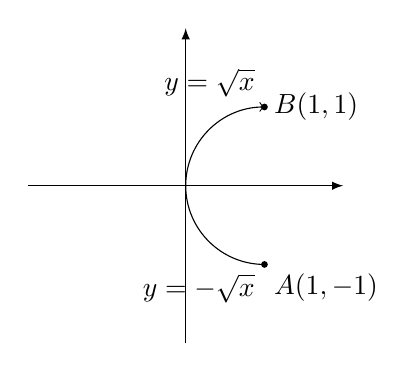
\begin{tikzpicture}
                \draw [-latex] (-2,0) -- (2,0);
                \draw [-latex] (0,-2) -- (0,2);
                \draw [->] (1,-1) node[below right]{$A(1,-1)$} node[below left]{$y = -\sqrt{x}$} arc (270:90:1) node[right]{$B(1,1)$} node[above left]{$y = \sqrt{x}$};
                \tikzPlaceDot{(1,-1)};
                \tikzPlaceDot{(1,1)};
              \end{tikzpicture}

              有两种方法 :
              \begin{enumerate}
                \item {
                      将$AB$分成两段,$A \to 0$和$0 \to B$ :
                      $$
                        \pathIntegral{L}xydx = \pathIntegral{A0}xydx + \pathIntegral{0B}xydx.
                      $$

                      因为在$A0$上$y = -\sqrt{x}$,在$0B$上$y = \sqrt{x}$,所以x的取值在$A0$上是$1 \to 0$,在$0B$上是$0 \to 1$.所以上式等于 :
                      $$
                        \definiteIntegral{0}{1}x(-\sqrt{x})dx + \definiteIntegral{1}{0}x(\sqrt{x})dx = 2\definiteIntegral{1}{x}x^{\cfrac{3}{2}}dx = \cfrac{4}{5}
                      $$

                      这可以形象的称为"按照x型区域积分"
                      }
                \item {
                      将公式变形成$x = y^2$ :

                      $\pathIntegral{L}y^2dx = \definiteIntegral{1}{-1}y^2 \cdot ydx = \definiteIntegral{1}{-1}y^2 \cdot y \cdot 2ydy = \cfrac{4}{5}$
                      }
              \end{enumerate}
              }
        \item{
              $\pathIntegral{L}y^2dx$,求沿着上半圆周L和从$A(a,0)$到$B(-a,0)$的直线$AB$的积分 :

              \begin{tikzpicture}
                \draw [-latex] (-3,0) -- (3,0);
                \draw [-latex] (0,-3) -- (0,3);
                \draw [->] (1.5,0) node [below right]{$A$} arc (0:180:1.5) node[below left]{$B$};
                \draw [->] (1.5,0) arc (0:90:1.5);
                \tikzPlaceDot{(-1.5,0)};
                \tikzPlaceDot{{(1.5,0)}};
              \end{tikzpicture}

              \begin{enumerate}
                \item {
                      第一题 : 极坐标 :
                      $$
                        x = a\cos\theta, y = a\sin\theta,0 \leq \theta \leq \pi \mbox{(注意旋转方向)}
                      $$
                      $$
                        \definiteIntegral{\pi}{0}a^2\sin^2\theta(-a\sin\theta)d\theta = a^3\definiteIntegral{\pi}{0}1 - \cos^2\theta d\cos\theta = -\cfrac{4}{3}a^3
                      $$
                      }
                \item {
                      第二题 : 沿着x轴,y始终等于0. x从$a$到$-a$ :
                      $$
                        \definiteIntegral{-a}{a}0^2dx = 0
                      $$
                      }
              \end{enumerate}
              }
      \end{enumerate}
    }%第二类曲线积分计算例题

    \subsubsection{两类曲线积分之间的联系}{
      先列出两类曲线积分的定义 :
      \begin{center}
        \begin{tabular}{c|c}
          第一类 :                                                       & 第二类                                                                                                              \\
          \hline
          {
            \begin{tikzpicture}
              \draw[-latex] (0,0) -- (3.5,0);
              \draw[-latex] (0,0) -- (0,3.5);

              \draw (1,1) node[left]{$A$} ..  controls (2,1) and (3,2) .. (4,4) node[right]{$B$};
              \draw (2.5,2) rectangle (3.5,2.5);
              \draw[-latex] (3.5,2.25) -- node[above]{切成小段并放大} (5.5,2.25);
              \draw (5.7,1.3) node[left]{$M_i - 1$} .. controls (6,1) and (7,2) .. node[below right]{$M(\xi_i,\eta_i)$} node[above left]{此段为$\Delta S_i$} (7,3) node[right]{$M_i$};
            \end{tikzpicture}
          }
                                                                         &
          {
              \begin{tikzpicture}
                \draw[-latex] (0,0) -- (3.5,0);
                \draw[-latex] (0,0) -- (0,3.5);

                \draw[->] (1,1) node[below left]{$A$} ..controls (1.5,3) and (3,3).. (4,4) node[right]{$B$};
                \draw (1.3,2) rectangle (1.8,2.5);
                \draw[-latex] (1.8,2.3) -- node[above]{切成小段并放大}(6,2.3);
                \draw[->] (6.2,2) node[left]{$M_i - 1$}  -- node[below right]{$F(\xi_i,\eta_i)$} (7.2,2.5) node[right]{$M_i$};
              \end{tikzpicture}
          }                                                                                                                                                                                    \\
          $\defFunction{\xi_i,\eta_i}\Delta S_i(\mbox{简称为}f\Delta S)$ & $P(\xi_i,\eta_i)\Delta x_i + Q(\xi_i,\eta_i)\Delta y_i(\mbox{简称为}P\Delta x + Q\Delta y)$                         \\
          $\downarrow$                                                   & $\downarrow$                                                                                                        \\
          {
          放大的积分弧段可以近似的看作一个三角形 :

          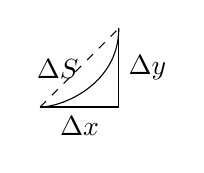
\begin{tikzpicture}
            \draw (0,0) -- node[below]{$\Delta x$} (1,0) -- node[right]{$\Delta y$} (1,1);
            \draw (0,0) ..controls (0.3,0) and (1,0.3).. node[above left]{$\Delta S$} (1,1);
            \draw[dashed] (0,0) -- (1,1);
          \end{tikzpicture}
          }
                                                                         &
          {
              将$P\Delta x + Q\Delta y$除以$\sqrt{\Delta x^2 + \Delta y^2}$
          }                                                                                                                                                                                    \\
          因此$f\Delta S = f\sqrt{\Delta x^2 + \Delta y^2}$              & 结果为$(P(\cfrac{\Delta x}{\sqrt{\Delta x^2 + \Delta y^2}}) + Q(\cfrac{\Delta y}{\sqrt{\Delta x^2 + \Delta y^2}}))$
        \end{tabular}
      \end{center}
      即 : $f = P(\cfrac{\Delta x}{\sqrt{\Delta x^2 + \Delta y^2}}) + Q(\cfrac{\Delta y}{\sqrt{\Delta x^2 + \Delta y^2}}) = P\cos\alpha + Q\cos\beta$\\

      设$x = \varphi(t),y = \psi(t)$,由此得出 :

      \begin{math}
        \definiteIntegral{\beta}{\alpha}(P(\varphi(t),\psi(t))\varphi\derivative(t) + Q(\varphi(t),\psi(t))\psi\derivative(t))dt \\
        = \definiteIntegral{\beta}{\alpha}(P\left(\varphi(t),\psi(t))\cfrac{\varphi\derivative(t)}{\sqrt{(\varphi\derivative(t))^2 + (\psi\derivative(t))^2}}+ Q(\varphi(t),\psi(t))\cfrac{\psi\derivative(t)}{\sqrt{(\varphi\derivative(t))^2 + (\psi\derivative(t))^2}}\right)\sqrt{(\varphi\derivative(t))^2 + (\psi\derivative(t))^2} \\
        = \definiteIntegral{\beta}{\alpha}(P(\varphi(t),\psi(t))\cos\alpha + Q(\varphi(t),\psi(t))\cos\beta)\sqrt{(\varphi\derivative(t))^2 + (\psi\derivative(t))^2} \\
        = \pathIntegral{L}[P(x,y)\cos\alpha + Q(x,y)\cos\beta]ds
      \end{math}
    }%两类曲线积分之间的联系

    \subsubsection{格林公式}{
      在物理学与数学中,格林公式给出了沿封闭曲线$C$的线积分与以$C$为边界的平面区域$D$上的双重积分的联系.格林公式是斯托克斯公式的二维特例 :

      设闭区域D由分段光滑的简单曲线$L$围成,函数$P(x,y)$及$Q(x,y)$在$D$上有一阶连续偏导数(即:没有洞的区域),则有 :
      $$
        \doubleIntegralOnZone{D}(\partialDerivativeFrac{Q}{x} - \partialDerivativeFrac{P}{y})dxdy = \curveIntegralOnLine{L^+}(Pdx + Qdy)
      $$

      其中$L^+$是$D$的取正向的边界曲线,$\oint$表示闭合路线上的曲线积分.
    }%格林公式结尾

    \subsubsection{当$D$为一个简单区域时格林公式的证明}{
      设一个比较简单的区域D,无论是沿着Y还是X都最多只有两个垂边,即 :
      \begin{center}
        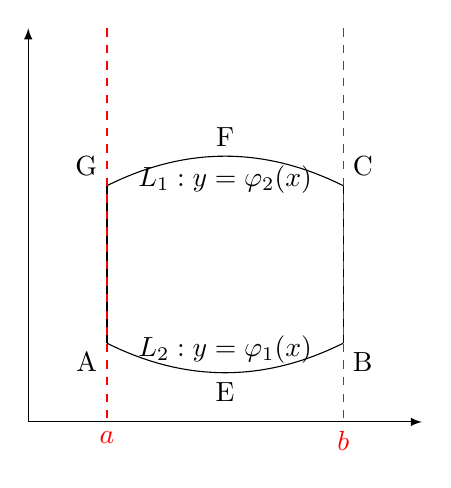
\begin{tikzpicture}
          \draw[-latex] (0,0) -- (0,5);
          \draw[-latex] (0,0) -- (5,0);
          \draw (1,3) node[above left]{G} -- (1,1) node[below left]{A};
          \draw (4,1) node[below right]{B} -- (4,3) node[above right]{C};
          \draw (1,3) ..controls (2,3.5) and (3,3.5).. node[above]{F} node[below]{$L_1 : y = \varphi_2(x)$} (4,3);
          \draw (1,1) ..controls (2,0.5) and (3,0.5).. node[below]{E} node[above]{$L_2 : y = \varphi_1(x)$}(4,1);
          \draw[color = red,dashed] (1,5) -- (1,0) node[below]{$a$};
          \draw[color = red,dashed] (4,5) -- (4,0) node[below]{$b$};
        \end{tikzpicture}
        \begin{tikzpicture}
          \draw[-latex] (0,0) -- (0,5);
          \draw[-latex] (0,0) -- (5,0);
          \draw (1,3) node[above left]{G} -- (1,1) node[below left]{A};
          \draw (4,1) node[below right]{B} -- (4,3) node[above right]{C};
          \draw (1,3) ..controls (2,3.5) and (3,3.5).. node[above]{F}(4,3);
          \draw (1,1) ..controls (2,0.5) and (3,0.5).. node[below]{E}(4,1);
          \draw[color = red,dashed] (5,3.35) -- (0,3.35) node[left]{$d$};
          \draw[color = red,dashed] (5,0.65) -- (0,0.65) node[left]{$c$};
          \node(A) at (4.2,4.5){设$\widehat{FGAE} : x = \psi_1(y),\widehat{EBCF} : x = \psi_2(y)$};
        \end{tikzpicture}
      \end{center}
      \begin{center}左:x型区域,右:y型区域\end{center}

      那么,区域$D$就可以写作:$D : \{(x,y)|\psi_1(y) \leq x \leq \psi_2(y),c \leq y \leq d\}$

      \begin{enumerate}
        \item {
              先证明后半部分 :
              $$
                \doubleIntegralOnZone{D}\partialDerivativeFrac{P}{y}dxdy = \definiteIntegral{b}{a}dx\definiteIntegral{\varphi_1(x)}{\varphi_2(x)}\partialDerivativeFrac{P}{y}dy = \definiteIntegral{b}{a}[P(x,\varphi_2(x)) - P(x,\varphi_1(x))]dx :
              $$

              \begin{math}
                \curveIntegralOnLine{L}Pdx \\
                = \pathIntegral{L_1}Pdx + \pathIntegral{BC}Pdx + \pathIntegral{L_2}Pdx + \pathIntegral{GA}Pdx \\
                = \pathIntegral{L_1}Pdx + \pathIntegral{L_2}Pdx \\
                = \definiteIntegral{b}{a}P(x,\varphi_1(x))dx + \definiteIntegral{a}{b}P(x,\varphi_2(x))dx \\
                = \definiteIntegral{b}{a}[P(x,\varphi_1(x)) - P(x,\varphi_2(x))]dx \\
                = -\doubleIntegralOnZone{D}\partialDerivativeFrac{P}{y}dxdy
              \end{math}
              }
        \item{
              然后是前半部分 :

              \begin{math}
                \doubleIntegralOnZone{D}\partialDerivativeFrac{Q}{x}dxdy \\
                = \definiteIntegral{d}{c}dy\definiteIntegral{\psi_2(y)}{\psi_1(y)}\partialDerivativeFrac{Q}{x}dx \\
                = \definiteIntegral{d}{c}[Q(\psi_2(y),y) - Q(\psi_1(y),y)]dy \\
                = \pathIntegral{L_2}Qdy + \pathIntegral{L_1}Qdy \\
                = \curveIntegralOnLine{L}Qdy
              \end{math}
              }
      \end{enumerate}
    }%当D时一个简单区域时格林公式的证明

    \subsubsection{格林公式的计算}{
      $$
        \doubleIntegralOnZone{D}\mediumBigCase{\partialDerivativeFrac{Q}{x} - \partialDerivativeFrac{P}{y}}dxdy = \curveIntegralOnLine{L}Pdx + Qdy
      $$

      有两种情况 :
      \begin{enumerate}
        \item {
              已经得知了以上公式的右侧,求左侧 (计算区域面积):
              使用格林公式,可以用线积分计算区域的面积.因为区域$D$的面积$A = \doubleIntegralOnZone{D}1dA$,所以只要选取适当的$P$与$Q$使得$\partialDerivativeFrac{Q}{x} - \partialDerivativeFrac{P}{y} = 1$,就可以通过$A = \curveIntegralOnLine{L}(Pdx + Qdy)$来计算面积.

              还有一种可能的取值是$A = \curveIntegralOnLine{L}xdy = -\curveIntegralOnLine{L}ydx = \cfrac{1}{2}\curveIntegralOnLine{L}(-ydx + xdy)$

              即 : 设$P = -y,Q = x,\partialDerivativeFrac{Q}{x} = 1,\partialDerivativeFrac{P}{y} = -1$

              那么$2\doubleIntegralOnZone{D}dxdy = \curveIntegralOnLine{L}xdy - ydx$

              所以$A = \cfrac{1}{2}\curveIntegralOnLine{L}xdy - ydx$

              $A$:积分区域面积
              }
        \item {
              已经得知了左侧,求右侧 :

              有以下例子 :
              \begin{enumerate}
                \item {
                      $$
                        \curveIntegralOnLine{L}x^2ydx - xy^2dy
                      $$
                      L : 正向圆周$x^2 + y^2 = a^2$.

                      $P = x^2y,Q =-xy^2,\partialDerivativeFrac{Q}{x} - \partialDerivativeFrac{P}{y} = -y^2-x^2$

                      原式$=\doubleIntegralOnZone{D}(-y^2-x^2)dxdy = -\definiteIntegral{2\pi}{0}d\theta\definiteIntegral{a}{0}\rho^2\rho d\rho = -\cfrac{\pi}{2}a^4$
                      }
                \item {
                      $\doubleIntegralOnZone{D}e^{-y^2}dxdy$,积分区域D : 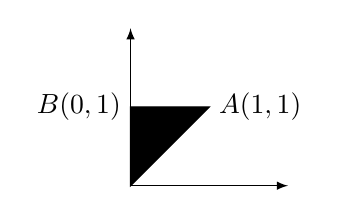
\begin{tikzpicture}
                        \draw[-latex] (0,0) -- (0,2);
                        \draw[-latex] (0,0) -- (2,0);
                        \filldraw[color = black] (0,0) -- (1,1) node[right]{$A(1,1)$} -- (0,1) node[left]{$B(0,1)$} -- cycle;
                      \end{tikzpicture}

                      设$P = 0,Q = xe^{-y^2}$

                      原式 = \begin{math}
                        \curveIntegralOnLine{OA + AB + BO}xe^{-y^2}dy \\
                        =\pathIntegral{OA}xe^{-y^2}dy \\
                        =\definiteIntegral{1}{0}xe^{-x^2}dx \\
                        =\cfrac{1}{2}(1 - e^{-1})
                      \end{math}

                      注 : $OA$直线是$y = x$
                      }
                \item {
                      $$
                        x = a\cos\theta,y = a\sin\theta,\mbox{求面积}
                      $$

                      用之前得出的$A = \cfrac{1}{2}\curveIntegralOnLine{L}xdy - ydx$ :

                      \begin{math}
                        \cfrac{1}{2}\definiteIntegral{2\pi}{0}(a\cos\theta \cdot a\cos\theta + a\sin\theta \cdot a\sin\theta)d\theta \\
                        =\pi ab
                      \end{math}
                      }
                \item {
                      $$
                        \curveIntegralOnLine{L}\cfrac{xdy - ydx}{x^2 + y^2},L:\mbox{无重点,分段光滑,且不过原点的连续闭曲线,方向逆时针.}
                      $$

                      $$
                        P=\cfrac{-y}{x^2 + y^2},Q=\cfrac{x}{x^2+y^2}\quad \partialDerivativeFrac{P}{y} = \partialDerivativeFrac{y^2 - x^2}{(x^2 +y^2)^2} = \partialDerivativeFrac{Q}{x}
                      $$

                      分两种情况 :
                      \begin{enumerate}
                        \item {
                              不包含原点,一阶偏导数存在且连续,$ \curveIntegralOnLine{L}\cfrac{xdy - ydx}{x^2 + y^2} = 0$ :
                              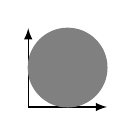
\begin{tikzpicture}
                                \draw[-latex] (0,0) -- (0,1);
                                \draw[-latex] (0,0) -- (1,0);
                                \filldraw[color = gray] (0.5,0.5) circle (0.5);
                              \end{tikzpicture}
                              }
                        \item{
                              包括原点,取适当小的$r > 0$,在原点附近作圆,圆周$C: x^2 + y^2 = r^2$,称为复联通区域,方向逆时针,用于代换原区域.

                              \begin{center}
                                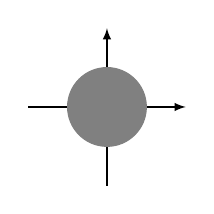
\begin{tikzpicture}
                                  \draw[-latex] (-1,0) -- (1,0);
                                  \draw[-latex] (0,-1) -- (0,1);
                                  \filldraw[color = gray] (0,0) circle (0.5);
                                \end{tikzpicture}
                              \end{center}
                              $$
                                \curveIntegralOnLine{L}\cfrac{xdy - ydx}{x^2 + y^2} - \curveIntegralOnLine{C}\cfrac{xdy - ydx}{x^2 + y^2} = 0
                              $$

                              $$
                                \curveIntegralOnLine{L}\cfrac{xdy - ydx}{x^2 + y^2} = \curveIntegralOnLine{C}\cfrac{xdy - ydx}{x^2 + y^2} = \definiteIntegral{2\pi}{0}\cfrac{r\cos\theta \cdot r\cos\theta + r\sin\theta \cdot r\sin\theta}{r^2}d\theta = 2\pi
                              $$
                              }
                      \end{enumerate}
                      }
              \end{enumerate}
              }
      \end{enumerate}
    }%格林公式的计算

  }%曲线积分与曲面积分结尾

  \subsection{雅可比矩阵与雅可比行列式}{
    在向量分析(多元微积分)中,雅可比矩阵是函数的一阶偏导数以一定方式排列成的矩阵。

    其重要性在于,如果函数 $f:\mathRealNumberCollection^n \to \mathRealNumberCollection^m$在点$x$可微的话,在点$x$的雅可比矩阵即为该函数在该点的最佳线性逼近,也代表雅可比矩阵是单变数实数函数的微分在向量值多变数函数的推广,在这种情况下,雅可比矩阵也被称作函数$f$在点$x$的微分或者导数.

    \subsubsection{雅可比矩阵}{
      假设某函数从$f : \mathRealNumberCollection^n \to \mathRealNumberCollection^M$,从$x\in\mathRealNumberCollection^n$映射到$\defFunction{x}\in\mathRealNumberCollection^m$,其雅可比矩阵就是一个$m \times n$的矩阵.换句话讲也就是从$\mathRealNumberCollection^n$到$\mathRealNumberCollection^m$的线性映射,其重要意义在于它表现了一个多变量向量函数的最佳线性逼近.因此,雅可比矩阵类似于单变数函数的导数.

      此函数$f$的雅可比矩阵$J$为$m \times n$的矩阵,一般由以下方式定义 :
      $$
        J =
        \begin{bmatrix}
          \partialDerivativeFrac{f}{x_1} & \dotsm & \partialDerivativeFrac{f}{x_n}
        \end{bmatrix}
        =
        \begin{bmatrix}
          \partialDerivativeFrac{f_1}{x_1} & \dotsm & \partialDerivativeFrac{f_1}{x_n} \\
          \vdots                           & \ldots & \vdots                           \\
          \partialDerivativeFrac{f_m}{x_1} & \dotsm & \partialDerivativeFrac{f_m}{x_n}
        \end{bmatrix}
      $$

      矩阵的分量可表示成 :
      $$
        J_{ij} = \partialDerivativeFrac{f_i}{x_j}
      $$

      雅可比矩阵的其他常用符号还有 :
      $$
        Df,J_f(x_1,\dots,x_n)\mbox{或者}\partialDerivativeFrac{(f_1,\dots,f_m)}{(x_1,\dots,x_n)}
      $$

      此矩阵的第$i$行是由函数$f_i$的梯度函数所表示的,$1 \leq i \leq m$.

      如果$p$是$\mathRealNumberCollection^n$中的一点,$f$在$p$点可微,根据数学分析,$J_f(p)$时在这点的导数.在此情况下,$J_f(p)$这个线性映射即$f$在点$p$附近的最佳线性逼近,也就是说当$x$足够靠近点p时,有 :
      $$
        \defFunction{x} \approx \defFunction{p} + J_f(p)\cdot(x - p)
      $$
      讲更详细点也就是 :
      $$
        \defFunction{x} = \defFunction{p} + J_f(p)(x - p) + \smallO{\doubleAbsoluteValue{x - p}}
      $$

      其中,$o$表示高阶无穷小,$\doubleAbsoluteValue{x - p}$为$x$与$p$之间的距离
    }%雅可比矩阵结尾

    \subsubsection{雅可比行列式}{
      当雅可比矩阵为方阵时,其行列式称为雅可比行列式.

      如果$m = n$,那么$f$是从$\mathRealNumberCollection^n$映射到$\mathRealNumberCollection^m$的函数,且他的雅可比矩阵是一个方阵.因此可以取他的行列式,称为雅可比行列式.

      在某个给定点的雅可比行列式提供了$f$在接近该点时的表现的重要资讯.例如:如果连续可微函数$f$在$p$点的雅可比行列式不等于0,那么他在该点附近有$f$的反函数,这成为反函数定理.更进一步,如果$p$点的雅可比行列式是正数,则$f$在$p$点保持定向.如果是负数,则逆转定向.而从雅可比行列式的绝对值,就可以知道函数$f$在$p$点附近时放大或缩小体积;这就是他出现在换元积分法中的原因.
    }%雅可比行列式结尾

    \subsubsection{举例}{
      \begin{enumerate}
        \item {
              球坐标系到直角坐标系的转化由$F : R^+\times[0,\pi]\times[0,2\pi) \to R^3$给出,其分量为 :
              $$
                \begin{array}{l}
                  x = r\sin\theta\cos\varphi \\
                  y = r\sin\theta\sin\varphi \\
                  z = r\cos\theta
                \end{array}
              $$

              此坐标变换的雅可比矩阵是 :
              $$
                J_F(r,\theta,\varphi)
                =
                \begin{bmatrix}
                  \partialDerivativeFrac{x}{r} & \partialDerivativeFrac{x}{\theta} & \partialDerivativeFrac{x}{\varphi} \\
                  \partialDerivativeFrac{y}{r} & \partialDerivativeFrac{y}{\theta} & \partialDerivativeFrac{y}{\varphi} \\
                  \partialDerivativeFrac{z}{r} & \partialDerivativeFrac{z}{\theta} & \partialDerivativeFrac{z}{\varphi}
                \end{bmatrix}
                =
                \begin{bmatrix}
                  \sin\theta\cos\varphi & r\cos\theta\cos\varphi & -r\sin\theta\sin\varphi \\
                  \sin\theta\sin\varphi & r\cos\theta\sin\varphi & r\sin\theta\cos\varphi  \\
                  \cos\theta            & -r\sin\theta           & 0
                \end{bmatrix}
              $$

              其雅可比行列式为$r^2\sin\theta$,由于$dV = dxdydz$,如果左变数变换的画其体积元$dV$会变成 : $dV = r^2\sin\theta dr d\theta d\varphi$.
              }
        \item {
              设有函数$F : R^3 \to R^3$,其分量为 :
              $$
                \begin{array}{l}
                  y_1 = 5x_2                   \\
                  y_2 = 4x_1^2 - 2\sin(x_2x_3) \\
                  y_3 = x_2x_3
                \end{array}
              $$

              则他的雅可比行列式为 :
              $$
                \begin{vmatrix}
                  0    & 5                 & 0                 \\
                  8x_1 & -2x_3\cos(x_2x_3) & -2x_2\cos(x_2x_3) \\
                  0    & x_3               & x_2
                \end{vmatrix}
                =
                -8x_1
                \cdot
                \begin{vmatrix}
                  5   & 0   \\
                  x_3 & x_2
                \end{vmatrix}
                =
                -40x_1x_2
              $$
              可以得出:当$x_1$与$x_2$同号时,$F$逆转定向;改函数处处具有反函数,除了在$x_1 = 0$或者$x_2 = 0$的点.
              }
      \end{enumerate}
    }%举例结尾

  }%雅可比矩阵与雅可比行列式结尾

}%多元微积分结尾

\section{无穷级数}{
在数学中,一个有穷或无穷的序列$u_{1},u_{2},u_{3},u_{4}\ldots$的和$S=u_{1}+u_{2}+u_{3}+\ldots$称为级数.如果序列是有穷序列,其和称为有穷级数;反之,称为无穷级数(一般简称为级数).序列{$u_{0},u_{1},u_{2},\ldots$中的项称作级数的通项(或一般项).级数的通项可以是实数,矩阵或向量等常量,也可以是关于其他变量的函数,不一定是一个数.一般的,如果级数的通项是常量,则称之为常数项级数,如果级数的通项是函数,则称之为函数项级数.

有穷数列的级数一般通过初等代数的方法就可以求得.无穷级数有发散和收敛的区别,称为无穷级数的敛散性.判断无穷级数的敛散性是无穷级数研究中的主要工作.无穷级数在收敛时才会有一个和;发散的无穷级数在一般意义上没有和,但可以用一些别的方式来定义.

$$
  \upDownSum{n}{i = 1}u_i = u_1 + u_2 + u_3 + \dots + u_n +  \dots
$$

其中$u_n$称为一般项,前$n$项之和$S_n = u_1 + u_2 + u_3 + u_n$称为部分和,比如 :
$$
  S_1 = u_1\qquad S_2 = u_1 + u_2\qquad S_3 = u_1 + u_2 + u_3 \dots
$$

当$\limNormal{n \to +\infty}S_n = S$,即趋于某个常数,就称此级数是收敛的.否则就是发散的.

设$S$是所有项的和,$S_n$是前$n$项的和,那么$R_n = S - S_n = u_{n+1} + u_{n + 2} + \dots$就被称为余项.

\subsection{无穷级数的性质}{
  无穷级数有以下性质 :
  \begin{itemize}
    \item $\sumSeries u_n$收敛于$s$则$\sumSeries ku_n$收敛于$ks$(即 : 级数的每一项乘以$k$不会改变敛散性.和也会乘以$k$)
    \item {
          $\sumSeries u_n$和$\sumSeries v_n$分别收敛于$s_1$和$s_2$,则$\sumSeries (u_n \pm v_n)$也收敛,且和等于$s_1 \pm s_2$.即 :
          \begin{itemize}
            \item 两个收敛的级数,相加减后仍收敛.
            \item 相加减后收敛的两个级数,本身未必收敛.
            \item 若两个级数都是绝对收敛,则合在一起也是绝对收敛.
            \item 若两个级数都是条件收敛,则合在一起可能是条件收敛,也可能是绝对收敛.
            \item 若两个级数一个是绝对收敛,一个是条件收敛,则合在一起是条件收敛.
          \end{itemize}
          }
    \item 去掉,加上或改变有限项,敛散性不变
    \item $\sumSeries u_n$收敛,任意加括号后得到的级数也收敛,并且和不变.(加括号后收敛,原级数不一定收敛)
    \item 级数$\sumSeries u_n$收敛的必要条件是$u_n$(即通项趋于0).(注意,是必要条件而非充分条件,即 : $u_n$趋于0,级数未必收敛,$u_n$不趋于0,级数一定发散)
  \end{itemize}
}%无穷级数的性质结尾

\subsection{常数项无穷级数审敛法}{
  常数项级数,即每一项都是常数的级数.

  \subsubsection{正项级数}{
    若通项为实数的无穷级数$\sum u_n$每一项$u_n$都大于等于零,则称$\sum u_n$是一正项级数.

    正项级数的部分和$S_n$是一个单调递增数列.由数列极限的判别准则:单调有界数列必有极限.因此,要么部分和数列$S_n$有界,这时$\sum u_n$收敛,$\myLimToInf S_n = s$,要么部分和数列趋于正无穷,这时级数发散.

    \begin{itemize}
      \item {
            比较判别法 :

            设$\sum u_n$和$\sum v_n$是正项级数.
            如果存在正实数$M$,使得从若干项开始,$u_n \leq Mv_n$(也就是说$u_n$是$v_n$的高阶无穷小),则 :
            \begin{itemize}
              \item 当$\sum v_n$收敛时,可推出$\sum u_n$也收敛.
              \item 当$\sum u_n$发散时,可推出$\sum v_n$也发散.
            \end{itemize}

            使用此方法常常是对所要判别的级数的通项进行放缩.

            比较判别法的特点是要已知若干级数的敛散性.一般来说,可以选择比较简单的级数:$P$级数$U_p = \sum\cfrac{1}{n^p}$作为"标准级数",依此判断其他函数的敛散性.需要知道的是当$p \leq 1$时,$P$级数发散.当$p \geq 1$时,$P$级数收敛.

            比如:已知级数$\sum \cfrac{1}{n^2}$收敛,则级数$\sum \cfrac{\absoluteValue{\sin n}}{n^2}$也收敛,因为对任意的$n$,$\sin n \leq 1$
            }
      \item{
            比较判别法的极限形式 :

            如果$\myLimToInf\cfrac{u_n}{v_n} = 1$或其他有限数,即同阶无穷小时,两者敛散性一致

            如果$\myLimToInf\cfrac{u_n}{v_n} = 0$,则 :
            \begin{itemize}
              \item 当$\sum v_n$收敛时,可推出$\sum u_n$也收敛.
              \item 当$\sum u_n$发散时,可推出$\sum v_n$也发散.
            \end{itemize}

            如果$\myLimToInf\cfrac{u_n}{v_n} = \infty$,则 :
            \begin{itemize}
              \item 当$\sum u_n$收敛时,可推出$\sum v_n$也收敛.
              \item 当$\sum v_n$发散时,可推出$\sum u_n$也发散.
            \end{itemize}

            注 : 使用此方法常常是采用等价无穷小替换或与$p$级数作比较,寻找同阶无穷小来判别原级数的敛散性。
            }
      \item{
            达朗贝尔判别法 :

            在比较判别法中,如果去几何级数为比较的标准级数,可得 :

            设$\sum u_n$是通项大于零的正项级数.且$\myLimToInf \cfrac{u_{n + 1}}{u_n} = p$,则 :
            \begin{itemize}
              \item 当$p < 1$时,级数$\sum u_n$收敛.
              \item 当$p > 1$时,级数$\sum u_n$发散.
              \item 当$p = 1$时,无法判断.级数$\sum u_n$可能收敛也可能发散
            \end{itemize}

            这个判别法也被称为比值判别法或者比值审敛法.

            对于多个式子连乘的,适合用此方法.
            }
      \item {
            柯西收敛准则 :

            设$\sum u_n$时正项级数.并且$\myLimToInf \sqrt[n]{u_n} = p$,则 :
            \begin{itemize}
              \item 当$p < 1$时,级数$\sum u_n$收敛.
              \item 当$p > 1$时,级数$\sum u_n$发散.
              \item 当$p = 1$时,级数$\sum u_n$可能收敛也可能发散.
            \end{itemize}

            这个判别法也称为根值判别法或根值审敛法.

            对于通项中含有以$n$为指数幂的,适合用此方法.
            }
      \item{
            对数判别法 :

            \begin{itemize}
              \item 若存在$\alpha > 0$,使当$n \geq n_0$时,$\cfrac{\ln\cfrac{1}{a_n}}{\ln n} \geq 1 + \alpha$,则正项级数$\sumSeries a_n$收敛.
              \item 若$n \geq n_0$时,$\cfrac{\ln\cfrac{1}{a_n}}{\ln n} \leq 1$,则正项级数$\sumSeries a_n$发散.
            \end{itemize}
            }
      \item {
            积分判别法 :

            若函数$\defFunction{x}$是区间$\mediumBigCase{a,+\infty}$上非负且单调递减的连续函数,则$\upDownSum{\infty}{n = a} a_n = \upDownSum{\infty}{n = a} f(n)$与$\definiteIntegral{a}{+\infty}\defFunction{x}dx$的敛散性一致.

            注意:只是敛散性一致.
            }
    \end{itemize}
  }%正项级数结尾

  \subsubsection{交错级数}{
    具有以下形式的级数 :
    $$
      \sumSeries (-1)^na_n\ (a_n >= 0)
    $$
    被称为交错级数.

    \begin{itemize}
      \item {
            莱布尼茨判别法 :

            在上述的级数$\sumSeries (-1)^na_n$中,如果当$n$趋于无穷时,数列$a_n$的极限存在且等于$0$,并且每个$a_n$小于$a_{n-1}$(即:数列$a_n$是单调递减的),那么级数收敛.

            即 : 交错级数$\sumSeries(-1)^{n}u_n$满足 :
            \begin{itemize}
              \item $u_{n - 1} > u_n$
              \item $\limNormal{n \to \infty}u_n = 0$
              \item 注:此处所指的$u_n,u_{n + 1}$不包括负号
            \end{itemize}
            }
      \item{
            利用级数的敛散性定义 :

            研究交错级数的部分和数列是否收敛,若部分和数列收敛,则级数收敛,反之发散.
            }
      \item{
            利用加括号级数判断 :

            \begin{itemize}
              \item 若加括号的级数发散,则原级数必发散
              \item 若加括号的级数收敛,且原级数的通项的极限为$0$,则原级数收敛.
            \end{itemize}
            }
      \item 拆通项判别
      \item {
            交换奇偶项判别:

            常常是交换奇偶项配合莱布尼兹判别法判别.
            }
    \end{itemize}
  }%交错级数结尾

  \subsubsection{任意项级数}{

    \begin{itemize}
      \item {
            比较判别法(只能判定收敛) :

            对于通项为任意实数的无穷级数$\sum u_n$,将级数$\sum \absoluteValue{u_n}$称为他的绝对值级数.可以证明,如果$\sum \absoluteValue{u_n}$收敛,那么$\sum u_n$也收敛,这时称$\sum u_n$为绝对收敛.如果$\sum u_n$收敛,但是$\sum \absoluteValue{u_n}$发散,则称$\sum u_n$为条件收敛.

            比如说,级数$\sum \cfrac{\sin n}{n^2}$绝对收敛,因为$\sum \cfrac{\absoluteValue{\sin n}}{n^2}$是收敛的,而级数$\sum \cfrac{(-1)^n}{n}$是条件收敛的.它自身收敛到$\ln\cfrac{1}{2}$,但是他的绝对值函数$\sum \cfrac{1}{n}$是发散的.
            }
      \item {
            比值判别法,根值判别法 :

            若$\limNormal{n \to \infty} \absoluteValue{\cfrac{a_{n + 1}}{a_n}} = \rho$或者$\limNormal{n \to \infty}\sqrt[n]{\absoluteValue{a_n}} = \rho$,则$\rho < 1$时收敛且为绝对收敛,$\rho > 1$时发散.
            }
    \end{itemize}

    黎曼级数定理说明,如果一个无穷级数$\sum u_n$条件收敛,那么对于任意的实数$x$,存在一个正整数到正整数的双射$\sigma$,使得级数$\sum u_{\sigma(n)}$收敛到$x$,对于正负无穷大,上述双射也存在.
  }%任意项级数结尾

  \subsubsection{常见常数项无穷级数}{

    \begin{itemize}
      \item {
            几何级数 :

            几何级数(或等比级数)是指通向为等比数列的级数,比如 :
            $$
              1 + \cfrac{1}{2} + \cfrac{1}{4} + \cfrac{1}{8} + \dots = \upDownSum{\infty}{n = 0} \cfrac{1}{2^n} = 2
            $$

            一般来说,几何级数$\upDownSum{\infty}{n = 0}z^n$收敛当且仅当$\absoluteValue{z} < 1$.
            }
      \item{
            调和级数 :

            调和级数是指通向为$\cfrac{1}{n}$的级数 :
            $$
              1 + \cfrac{1}{2} + \cfrac{1}{3} + \dots = \sumSeries \cfrac{1}{n}
            $$

            他是发散的.
            }
      \item{
            $p$级数 :

            指通项为$\cfrac{1}{n^p}$的级数 :
            $$
              U_p = \sumSeries\cfrac{1}{n^p}
            $$

            对于实数值$p$,当$p > 1$时收敛,$p <= 1$时发散,$p = 1$时为调和级数.
            }
      \item{
            列项级数 :
            $$
              \sumSeries(b_n - b_{n - 1})
            $$

            收敛当且仅当数列$b_n$收敛到某个极限$L$,这时级数的和是$b_1 - L$.
            }
      \item{
            交错级数 :

            具有以下形式的级数 :
            $$
              \upDownSum{\infty}{n = 0}(-1)^na_n
            $$

            其中所有的$a_n$非负,就被称为交错级数.
            }
    \end{itemize}

  }%常见常数项无穷级数结尾

}%常数项无穷级数审敛法

\subsection{函数项无穷级数审敛法}{
设$(u_n(x))_{n \geq 0}$为定义在区间$I$上的函数列,则表达式$u_1(x) + u_2(x) + \dots + u_n(x) + \dots$称为函数项级数,记为$\sum u_n(x)$.对函数项级数的主要研究是 :
\begin{enumerate}
  \item 确定对哪些$x,\sum u_n(x)$收敛
  \item $\sum u_n(x)$收敛的话,其和是什么,有什么性质?
\end{enumerate}

\subsubsection{一些定义(收敛点,收敛域,发散点,发散域,和函数与部分和还有余项)}{
  对于区间$I$上的每个点$x_0$,级数$\sum u_n(x_0)$是常数项级数.
  \begin{itemize}
    \item 收敛点 : 若$\sum u_n(x_0)$收敛,则称$x_0$是$\sum u_n(x)$的一个收敛点.
    \item 收敛域 : $\sum u_n(x)$全体收敛点的集合称为他的收敛域.
    \item 发散点 : 若$\sum u_n(x_0)$发散,则称$x_0$是$\sum u_n(x)$的一个发散点.
    \item 发散域 : $\sum u_n(x)$全体发散点的集合称为他的发散域.
    \item $\sum u_n(x)$在其收敛域的每一点上都有定义,因此定义了一个函数,称为$\sum u_n(x)$的和函数,记为$S(x)$.
    \item $S(x_0) = \limNormal{n \to \infty}S_n(x_0)$,其中$S_n(x_0) = u_1(x_0) + u_2(x_0) + \dots + u_n(x_0)$为函数项级数在$x_0$点上的部分和.
    \item 余项为和函数减去部分和 : $r_n(x) = S(x) - S_n(x)$,显然 : $\limNormal{n \to \infty} r_n(x) = 0$
  \end{itemize}
}%收敛域结尾

\subsubsection{阿贝尔定理}{
  设$\defFunction{z} = \upDownSum{\ }{n \geq 0}a_nx^n$为一幂级数,其收敛半径为$R$,若对于收敛圆(模长为$R$的复数的集合)上的某个复数$z_0$,级数$\upDownSum{\ }{n \geq 0}a_nx^n_0$收敛,则有 : $\limNormal{t \to 1^-}\defFunction{tx_0} = \upDownSum{\ }{n \geq 0}a_nx^n_0$.

  用人话来说就是 : $\upDownSum{+\infty}{n = 0}a_nx^n$,如果$x = x_0$时此幂级数收敛,对于所有满足$\absoluteValue{x} \leq \absoluteValue{x_0}$的$x$,此幂级数绝对收敛.反之,如果$x = x_0$时发散,则对于所有满足$\absoluteValue{x} > \absoluteValue{x_0}$的$x$,此幂级数发散.

  收敛半径是指收敛圆的半径,在数轴上是指收敛域的半径.

  推论 : 收敛的情况有这三种 :
  \begin{itemize}
    \item $x = 0$时收敛
    \item $x \in (-\infty,+\infty)$时收敛.
    \item $\absoluteValue{x} < R$时绝对收敛(在端点处可能发散也可能收敛).
  \end{itemize}
  在判断端点(是否收敛)之前$(-R,R)$称为收敛区间,经过判断决定了是否保留端点后才称为收敛域.
}

\subsubsection{求幂级数的收敛域}{
  设幂级数$\sum a_nx^n$满足$\limNormal{n \to +\infty}\cfrac{a_{n + 1}}{a_n} = \rho$,则 :
  \begin{itemize}
    \item $\rho$是正实数时,$R = \cfrac{1}{p}$.
    \item $\rho = 0$时,$R = \infty$
    \item $\rho = \infty$时,$R = 0$
  \end{itemize}

  如果模糊一下概念,可以概括为:$R = \cfrac{1}{\rho}$.

  注 : 如果只有偶数项则不能用此方法.
}%求幂级数的收敛域结尾

\subsubsection{幂级数的比值审敛法}{
$$
  \limNormal{n \to +\infty}\absoluteValue{\cfrac{u_{n + 1}}{u_n}} = L
$$

求当$x$为何值时$L < 1$

例 :
求$\upDownSum{+\infty}{n = 0}\cfrac{(2n)!}{(n!)^2}x^{2n}$的收敛半径 : $$
  \limNormal{n \to +\infty}\absoluteValue{\cfrac{\cfrac{(2(n + 1))!}{((n + 1)!)^2}x^{2n + 2}}{\cfrac{(2n)!}{(n!)^2}x^{2n}}} = 4\absoluteValue{x}^2 < 1,\ \absoluteValue{x} < \cfrac{1}{2},\ R = \cfrac{1}{2}
$$
}

\subsubsection{幂级数的运算}{
  \begin{itemize}
    \item {
          幂级数的加法与减法 : 将相应系数进行加减.
          \begin{math}
            (a_0+ a_1x + a_2x^2 + \dots + a_nx^n + \dots) \pm (b_0 + b_1x + b_2x^2 + \dots + b_nx^n + \dots)
            = (a_0 + b_0) + (a_1 + b_1)x + (a_2 + b_2)x^2 + \dots + (a_n + b_n)x^n + \dots
          \end{math}
          }
    \item {
          幂级数的乘积 : 基于柯西乘积

          \begin{math}
            $$\bigCase{\upDownSum{\infty}{n = 0}a_n(x - c)^n}\mediumBigCase{\upDownSum{\infty}{n = 0}b_n(x - c)^n}$$ \\
            = \upDownSum{\infty}{i = 0}\upDownSum{\infty}{j = 0}a_ib_j(x - c)^{i + j} \\
            = \upDownSum{\infty}{n = 0}\bigCase{\upDownSum{n}{i = 0}a_ib_{n - i}}(x - c)^n
          \end{math}

          举例 : $$
            \upDownSum{\infty}{n = 0}a_nx^n \times \upDownSum{\infty}{n = 0}b_nx^n = a_0b_0 + (a_0b_1 + a_1b_0)x + (a_0b_2 + a_1b_1 + a_2b_0)x^2 + \dots + (a_0b_n + a_1b_{n-1} + \dots + a_nb_0)x^n + \dots
          $$
          }
    \item{
          幂级数的除法 :

          两个幂级数相除的结果仍然是幂级数.假设$b_0 \neq 0$时 :
          $$
            \cfrac{a_0 + a_1x + a_2x^2 + \dots + a_nx^n + \dots}{b_0 + b_1x + b_2x^2 + \dots + b_nx^n + \dots} = c_0 + c_1x + c_2x^2 + \dots + c_nx^n + \dots
          $$

          系数$c_0,c_1,\dots,c_n$由以下等式逐一确立 :

          \begin{math}
            a_0 = b_0c_0 \\
            a_1 = b_1c_0 + b_0c_1 \\
            a_2 = b_2c_0 + b_1c_1 + b_0c_2 \\
            \dots \\
            a_n = b_nc_0 + b_{n-1}c_1 + \dots + b_0c_n
          \end{math}

          相除所得的幂级数的收敛域可能比原来两个幂级数的收敛域都小得多.
          }
  \end{itemize}

  在各种运算后得到的幂级数的收敛半径为较小者.
}%幂级数的运算结尾

\subsubsection{幂级数和函数的性质}{
  \begin{itemize}
    \item 幂级数$\upDownSum{\infty}{n = 0}a_nx^n$的和函数$s(x)$在其收敛域$I$上连续.
    \item {
          幂级数$\upDownSum{\infty}{n = 0}a_nx^n$的和函数$s(x)$在其收敛域上$I$可积,并有逐项积分公式 :
          $$
            \definiteIntegral{x}{0}s(x)dx = \definiteIntegral{x}{0}\bigCase{\upDownSum{\infty}{n = 0}a_nx^n}dx = \upDownSum{\infty}{n = 0}\definiteIntegral{x}{0}a_nx^ndx = \upDownSum{\infty}{n = 0}\cfrac{a_n}{n + 1}x^{n + 1},(x \in I)
          $$
          逐项积分后所得的幂级数和原函数有相同的收敛半径.收敛域端点要重新考察.

          推论 : 幂级数$\upDownSum{\infty}{n = 0}a_nx^n$的和函数$s(x)$在其收敛域内可逐项积分任意次.
          }
    \item{
          幂级数$\upDownSum{\infty}{n = 0}a_nx^n$的和函数$s(x)$在其收敛区间$(-R,R)$内可导,并有逐项求导公式 :
          $$
            是\derivative(x) = \bigCase{\upDownSum{\infty}{n = 0}a_nx^n}\derivative = \upDownSum{\infty}{0}(a_nx^n)\derivative = \upDownSum{\infty}{n = 1}na_{n - 1}x^{n - 1},(\absoluteValue{x} < R)
          $$
          逐项求导后所得的幂级数和原级数有相同的收敛半径.收敛域端点要重新考察.

          推论 : 幂级数$\upDownSum{\infty}{n = 0}a_nx^n$的和函数$s(x)$在其收敛区间$(-R,R)$内有任意阶导数.
          }

          实际应用举例 :
          求$\upDownSum{\infty}{n = 1}nx^{n - 1}$的收敛域,和函数,并求$\cfrac{n}{2^n}$ :
          $$
            \limNormal{n \to \infty}\absoluteValue{\cfrac{a_{n + 1}}{a_n}} = \limNormal{n \to \infty}\absoluteValue{\cfrac{n + 1}{n}} = 1 = \rho,R = \cfrac{1}{\rho} = 1
          $$
          因此$(-1,1)$为收敛区间,在端点处判断后可得出结论:收敛域为$(-1,1)$.

          设$s(x) = \upDownSum{\infty}{n = 1}nx^{n - 1}$

          \begin{math}
            \definiteIntegral{x}{0}s(x)dx
            = \definiteIntegral{x}{0}\upDownSum{\infty}{n = 1}nx^{n - 1}dx \\
            = \upDownSum{\infty}{n = 1}\definiteIntegral{x}{0}nx^{n - 1}dx \\
            = \upDownSum{\infty}{n = 1}x^n|^x_0 \\
            = \upDownSum{\infty}{n = 1}x^n \\
            =\cfrac{x}{1 - x}\ (\absoluteValue{x} < 1)
          \end{math}

          $S(x) = \cfrac{1}{1 - x^2},x \in (-1,1)$,$(\definiteIntegral{x}{0}S(x)dx)\derivative = S(x)$(变上限积分).

          令$x = \cfrac{1}{2},S(x) = \upDownSum{\infty}{n = 1}n\bigCase(\cfrac{1}{2})^{n - 1} = 4,\upDownSum{\infty}{n - 1}\cfrac{n}{2^n} = S(x)\times\cfrac{1}{2} = \cfrac{1}{2} \times 4 = 2$
  \end{itemize}

  关于这些性质的用法有以下五条建议 :
  \begin{itemize}
    \item 要先求导时,$n$最好在分母上,即$\cfrac{1}{n}$.
    \item 要先求积分时,$n$最好在分子上.
    \item 注意提出可以抵消的$x$的幂次方.
    \item 求几次积分就要求几次导,相反也一样.
    \item 可以适当的拆项.
  \end{itemize}
}%幂级数和函数的性质结尾

}%函数项无穷级数审敛法

\subsection{函数的幂级数展开(泰勒级数)}{
  假设有函数$f(x)$,想要展开成$a_0 + a_1(x - x_0) + a_2(x - x_0)^2 + a_3(x - x_0)^3 + \dots  + a_n(x - x_0)^n + \dots$的形式,其中$x$是$x_0$的极限,即 : \\
  \begin{math}
    \defFunction{x} = a_0 + a_1(x - x_0)^1 + a_2(x - x_0)^2 + \dots + a_n(x - x_0)^n + \dots \\
    \fDerivative{x} = 0 + a_1 + 2a_2(x - x_0) + 3a_3(x - x_0)^2 + \dots \\
    f\doubleDerivative(x) = 0 + 0 + 2a_2 + 2 \times 3 a_3(x - x_0) + 3 \times 4 a_4(x - x_0)^2 + \dots \\
    f\tripleDerivative(x) = 0 + 0 + 0 + 2 \times 3 a_3 + 3 \times 4 a_4(x - x_0) + \dots
  \end{math}

  将x取值成$x_0$,即$x = x_0$,代入 : \\
  \begin{math}
    \defFunction{x_0} = {\color{red}a_0} + 0 + 0 + 0 + 0 + \dots\ \to \ a_0 = \defFunction{x_0} \\
    \fDerivative{x_0} = 0 + {\color{red}a_1} + 0 + 0 + 0 + 0 + \dots\ \to \ a_1 = \fDerivative{x_0} \\
    f\doubleDerivative(x_0) = 0 + 0 + {\color{red}2a_2} + 0 + 0 + 0 + 0 + \dots\ \to \ a_2 = \cfrac{f\doubleDerivative(x_0)}{2!} \\
    f\tripleDerivative(x_0) = 0 + 0 + 0 + {\color{red}2 \times 3 a_3} + 0 + 0 + 0 + 0 + \dots\ \to \ a_3 = \cfrac{f\tripleDerivative(x_0)}{3!} \\
    \vdots
  \end{math}

  最后可以总结出公式 :
  $$
    a_n = \cfrac{1}{n!}f\aLotDerivative{n}(x_0),\ \defFunction{x} = \upDownSum{\infty}{n = 0}\cfrac{1}{n!}f\aLotDerivative{n}(x_0)(x - x_0)^n
  $$

  这种级数展开泰勒级数,此通项公式称为泰勒展开式.

  函数$f(x)$能展开成幂级数的充要条件就是 : 泰勒展开式成立,且收敛到$\defFunction{x}$.

  更确切的来说 :
  \subsubsection{泰勒展开式与马克劳林展开式}{
    泰勒展开式 :
    $$
      \defFunction{x} = \upDownSum{\infty}{n = 0}\cfrac{1}{n!}f\aLotDerivative{n}(x_0)(x - x_0)^n\qquad x\in U(x_0),\mbox{此公式在$x_0$的邻域内成立}
    $$

    当$x_0$取$0$,在$0$处展开,就称为马克劳林公式 :
    $$
      \defFunction{x} = \upDownSum{\infty}{n = 0}\cfrac{1}{n!}f\aLotDerivative{n}(0)x^n\qquad x\in I_{f},\mbox{麦克劳林的定义更加清晰:此公式在收敛域内成立}.
    $$
  }%泰勒展开式结尾

  \subsubsection{基础函数展开公式表推导}{
    注 : 此处全部使用马克劳林展开
    \begin{enumerate}
      \item {
            $\defFunction{x} = e^x$ :

            由于$f\aLotDerivative{n}(0) = 1$,而且$f\derivative = e$,因此展开项为 :
            $$
              e^x = 1 + x + \cfrac{x^2}{2!} + \dots + \cfrac{x^n}{n!} + \dots
            $$
            }
      \item {
            $\defFunction{x} = \sin(x),g(x) = \cos(x)$ :

            \begin{center}
              \begin{tabular}{c c}
                $\fDerivative{x} = \cos(x)$        & $\fDerivative{0} = 1$        \\
                $f\doubleDerivative(x) = -\sin(x)$ & $f\doubleDerivative(0) = 0$  \\
                $f\tripleDerivative(x) = \cos(x)$  & $f\tripleDerivative(0) = -1$ \\
                $f\aLotDerivative{4}(x) = \sin(x)$ & $f\aLotDerivative{4}(0) = 0$
              \end{tabular}
            \end{center}

            总结规律,可知 : 展开式只有奇数次项,并且正负会交替出现 :
            $$
              \sin(x) = x - \cfrac{x^3}{3!} + \cfrac{x^5}{5!} - \cfrac{x^7}{7!} + \dots + (-1)^n\cfrac{x^{2n + 1}}{(2n + 1)!} + \dots
            $$

            由$\fDerivative{x} = g(x)$,对上式求导就会得到$\cos$的展开式 :
            $$
              \cos(x) = 1 - \cfrac{x^2}{2!} + \cfrac{x^4}{4!} - \cfrac{x^6}{6!} + \dots + (-1)^n\cfrac{x^{2n}}{(2n)!} + \dots
            $$

            特点是只有偶次项.
            }
      \item {
            $\defFunction{x} = \cfrac{1}{1 - x}$ :

            很容易看出这是等比(几何)级数的通项公式 :
            $$
              \cfrac{1}{1 - x} =1 + x + x^2 + x^3 + \dots + x^n + \dots
            $$

            将$x$换成$-x$ :
            $$
              \cfrac{1}{1 + x} = 1 - x + x^2 - x^3 + x^4 + \dots + (-1)^nx^n + \dots
            $$

            上述两个公式在$\absoluteValue{x} < 1$时成立
            }
      \item{
            公式3从$0$到$x$求定积分 : $\definiteIntegral{x}{0}\cfrac{1}{1 - x}dx = \ln(1 - x),\definiteIntegral{x}{0}\cfrac{1}{1 + x}dx = \ln(1 + x)$ :

            $$
              \ln(1 - x) = -x - \cfrac{x^2}{2} - \cfrac{x^3}{3} - \dots - \cfrac{x^n}{n} - \dots
            $$

            $$
              \ln(1 + x) = x + \cfrac{x^2}{2} + \cfrac{x^3}{3} + \dots + \cfrac{x^n}{n} + \dots
            $$

            上述两个公式对于在区间$\left(-1,1\right]$内的所有x都成立.
            }
      \item {
            将公式1中的$x$换成$x\ln a$ : $e^{x\ln a} = a^x$ :

            $$
              a^x = 1 + x\ln a + \cfrac{x^2(\ln a)^2}{2!} + \cfrac{x^3(\ln a)^3}{3!} + \dots + \cfrac{x^n(\ln a)^n}{n!} + \dots
            $$
            }
      \item{
            将公式3中$\cfrac{1}{1 + x}$中的$x$换成$x^2$ : $\cfrac{1}{1 + x^2}$ :

            $$
              \cfrac{1}{1 + x^2} = 1 - x^2 + x^4 - x^6 + x^8 + \dots + (-1)^nx^{2n} + \dots
            $$

            同样的,对于在区间$\left(-1,1\right]$中的所有$x$成立.
            }
      \item {
            对公式7在$0$到$x$求定积分 : $\definiteIntegral{x}{0}\cfrac{1}{1 + x^2}dx = \arctan(x)$  :

            $$
              \arctan(x) = x - \cfrac{x^3}{3} + \cfrac{x^5}{5} - \cfrac{x^7}{7} + \dots + (-1)^n\cfrac{x^{2n + 1}}{2n + 1} + \dots
            $$

            对于所有$\absoluteValue{x} < 1$成立.
            }
    \end{enumerate}
  }%基础函数展开公式表推导

  \subsubsection{基础函数展开公式表}{
    \begin{itemize}
      \item $e^x = 1 + x + \cfrac{x^2}{2!} + \dots + \cfrac{x^n}{n!} + \dots,(-\infty < x < +\infty)$
      \item $\sin(x) = x - \cfrac{x^3}{3!} + \cfrac{x^5}{5!} - \cfrac{x^7}{7!} + \dots + (-1)^n\cfrac{x^{2n + 1}}{(2n + 1)!} + \dots,(-\infty < x < +\infty)$
      \item $\cos(x) = 1 - \cfrac{x^2}{2!} + \cfrac{x^4}{4!} - \cfrac{x^6}{6!} + \dots + (-1)^n\cfrac{x^{2n}}{(2n)!} + \dots,(-\infty < x < +\infty)$
      \item $\cfrac{1}{1 - x} = 1 + x + x^2 + x^3 + \dots + x^n + \dots,(-1 < x < 1)$
      \item $\cfrac{1}{1 + x} = 1 - x + x^2 - x^3 + x^4 + \dots + (-1)^nx^n + \dots,(-1 < x < 1)$
      \item $\ln(1 - x) = -x - \cfrac{x^2}{2} - \cfrac{x^3}{3} - \dots - \cfrac{x^n}{n} - \dots,(-1 < x \leq 1)$
      \item $\ln(1 + x) = x + \cfrac{x^2}{2} + \cfrac{x^3}{3} + \dots + \cfrac{x^n}{n} + \dots,(-1 < x \leq 1)$
      \item $a^x = 1 + x\ln a + \cfrac{x^2(\ln a)^2}{2!} + \cfrac{x^3(\ln a)^3}{3!} + \dots + \cfrac{x^n(\ln a)^n}{n!} + \dots,(-\infty < x < +\infty)$
      \item $\cfrac{1}{1 + x^2} = 1 - x^2 + x^4 - x^6 + x^8 + \dots + (-1)^nx^{2n} + \dots,(-1 < x \leq 1)$
      \item $\arctan(x) = x - \cfrac{x^3}{3} + \cfrac{x^5}{5} - \cfrac{x^7}{7} + \dots + (-1)^n\cfrac{x^{2n + 1}}{2n + 1} + \dots,(-1 < x < 1)$
    \end{itemize}
  }%基础函数展开公式表结尾

  \subsubsection{运算示例}{
    \begin{enumerate}
      \item {
            将$e^{\cfrac{x}{2}}$展开 :

            将$x$换成$\cfrac{x}{2}$,即 :
            $$
              e^{\cfrac{x}{2}} = 1 + \cfrac{x}{2} + \cfrac{x^2}{2!2^2} + \cfrac{x^3}{3!3^2} + \dots + \cfrac{x^n}{n!n^2}
            $$
            }
      \item {
            将$\defFunction{x} = (1 - x)\ln(1 + x)$展成$x$的幂级数 :
            $$
              \ln(1 + x) = x - \cfrac{x^2}{2} + \cfrac{x^3}{3} - \cfrac{x^4}{4} + \dots
            $$

            \begin{math}
              (1 - x)\ln(1 + x) \\
              = (1 - x)(x - \cfrac{x^2}{2} + \cfrac{x^3}{3} - \cfrac{x^4}{4} + \dots) \\
              = x + (-\cfrac{1}{2} - 1)x^2 + (\cfrac{1}{3} + \cfrac{1}{2})x^3 + (-\cfrac{1}{4} - \cfrac{1}{3})x^4 + \dots \\
              = x + \upDownSum{\infty}{n = 2}(-1)^{n - 1}\cfrac{(2n - 1)x^n}{n(n - 1)} \ (-1 < x \leq 1)
            \end{math}
            }
      \item {
            将$\sin x$展成$x - \cfrac{\pi}{4}$的幂级数.

            (泰勒级数在$\cfrac{\pi}{4}$处展开,也可以用马克劳林),使用马克劳林 :

            \begin{math}
              \sin x \xrightarrow{x \to x - \cfrac{\pi}{4}} \sin(\cfrac{\pi}{4} + x - \cfrac{\pi}{4}) \\
              = \sin\cfrac{\pi}{4}\cos(x - \cfrac{\pi}{4}) + \cos\cfrac{\pi}{4}\sin(x - \cfrac{\pi}{4}) \\
              = \cfrac{\sqrt{2}}{2}(\cos(x - \cfrac{\pi}{4}) + \sin(x - \cfrac{\pi}{4})) \\
              =\dots
            \end{math}
            }
      \item {
            将$\defFunction{x} = \cfrac{1}{x^2 + 4x + 3}$展成$x - 1$的幂级数 :
            $$
              \defFunction{x} = \cfrac{1}{(x + 1)(x + 3)} = \cfrac{1}{2}\bigCase{\cfrac{1}{1 + x} - \cfrac{1}{3 + x}}
            $$

            $$
              \cfrac{1}{1 + x} = \cfrac{1}{2 + (x - 1)} = \cfrac{1}{2}\bigCase{\cfrac{1}{1 + \cfrac{x - 1}{2}}}(\mbox{先凑出形式})
            $$

            令$\cfrac{x - 1}{2} = t$,对$\cfrac{1}{2}\cfrac{1}{1 + t}$展开 : $\cfrac{1}{2}\bigCase{1 - \cfrac{x - 1}{2} + \cfrac{(x - 1)^2}{2^2} - \cfrac{(x - 1)^3}{2^3} + \dots}$

            同理,$\cfrac{1}{3 + x}$经过变形 :
            $$
              \cfrac{1}{4}(\cfrac{1}{1 + \cfrac{x - 1}{4}}) = \cfrac{1}{4}\bigCase{1 - \cfrac{x - 1}{4} \cfrac{(x - 1)^2}{4^2} - \cfrac{(x - 1)^3}{4^3} + \dots}
            $$

            因此.$\defFunction{x} = \sumSeries(-1)^n\bigCase{2^{\cfrac{1}{n + 2}} - 2^{\cfrac{1}{2n + 3}}}(x - 1)^n$

            还需要求出收敛域 :

            $-1 < \cfrac{x - 1}{4} < 1 \to -3 < x < 5$,收敛域为$(-3 < x < 5)$

            $-1 < \cfrac{x - 1}{2} < 1 \to -1 < x < 3$,收敛域为$(-1 < x < 3)$

            两者相加减,收敛域取交集 : $(-3 < x < 5) \intersectionSet (-1 < x < 3) = (-1 < x < 3)$

            即 : $\defFunction{x}$收敛域为$(-1 < x < 3)$
            }
    \end{enumerate}
  }%运算示例结尾

}%函数的幂级数展开结尾

}%无穷级数结尾

\section{场论(含有多元微积分向量分析部分)}{

  \subsection{场论基本内容}{
    注:矢量 = 向量,有时候会混着用,一般是那个顺口用哪个.

    \subsubsection{矢量函数/向量函数}{
      向量值函数,有时也称为向量函数,是一个单变量或多变量的、值域是多维向量或者无穷维向量的集合的函数.向量值函数的输入可以是一个标量或者一个向量(定义域的维度可以是1或大于1);定义域的维度不取决于值域的维度.

      即:设有数性变量t和变矢量$\vec{A}$.若对于t在某个范围内的每一个数值,$\vec{A}$都有一个确定的矢量和它对应,则称$\vec{A}$为数性变量t的矢量函数.记为:$\vec{A} = A(t)$,也可以写作$\vec{A} = A_x(t)i + A_y(t)j + A_z(t)k$

      矢量函数$A(t)$的起点取在坐标原点,其终点随变量t变化描绘出了一条曲线,该曲线叫做$A(t)$的矢端曲线.也就是$A(t)$的图像.
    }%矢量函数/向量函数结尾

    \subsubsection{矢量向量函数的极限}{
      用$\delta-\epsilon$语言来说:

      设矢量函数$A(t)$在点$t_0$的某个邻域内有定义(在$t_0$点可以没有),$\vec{A}_0$为常矢量.若对于任意给定$\epsilon > 0$,都存在一个$\delta > 0$,当$0 < |t - t_0| < \delta$时,就有$|A(t) - \vec{A}_0|$成立,则称当$t \to t_0$时,$A(t)$有极限$\vec{A}_0$,记作:

      \begin{center}
        $\limNormal{t \to t_0}A(t) = \vec{A}_0$
      \end{center}

      注:在直角坐标系中有:

      \begin{center}
        $\limNormal{t \to t_0}A_x(t) = A_{0x}$ \\
        $\limNormal{t \to t_0}A_y(t) = A_{0y}$ \\
        $\limNormal{t \to t_0}A_z(t) = A_{0z}$
      \end{center}

      其中$\vec{A}_0 = A_{0x}\vec{i} + A_{0y}\vec{j} + A_{0z}\vec{k}$
    }%矢量函数的极限结尾

    \subsubsection{矢量函数的连续}{
      设$A(t)$在$t_0$的某领域内有定义,且 :

      \begin{center}
        $\limNormal{t \to t_0}A(t) = A(t_0)$
      \end{center}

      即 :

      \begin{center}
        $\limNormal{t \to t_0}A_x(t) = A_x(t_0)$ \\
        $\limNormal{t \to t_0}A_y(t) = A_y(t_0)$ \\
        $\limNormal{t \to t_0}A_y(t) = A_y(t_0)$
      \end{center}

      就称$A(t)$在$t_0$点连续.
    }%矢量函数的连续结尾

    \subsubsection{矢量函数的导数}{
      设矢量函数$A(t)$在点t处有增量$\Delta \vec{A} = A(t + \Delta t) - A(t)$

      当$\Delta t \to 0$时,$\cfrac{\Delta \vec{A}}{\Delta t} = \cfrac{A(t + \Delta t) - A(t)}{\Delta t}$的极限存在,则称此极限值为$A(t)$在点t处的导向量/导矢.即 :

      $$
        A\derivative(t) = \cfrac{dA(t)}{dt} = \limNormal{\Delta t \to 0}\cfrac{\Delta \vec{A}}{\Delta t} = \limNormal{\Delta t \to 0}\cfrac{A(t + \Delta t) - A(t)}{\Delta t}
      $$

      以下为导数公式 :

      \begin{itemize}
        \item $\cfrac{d}{dt}(\vec{\mathConstant}) = 0$ ($\vec{\mathConstant}$为常矢量)
        \item $\cfrac{d}{dt}(\vec{A} \pm \vec{B}) = \cfrac{d}{dt}\vec{A} \pm \cfrac{d}{dt}\vec{B}$
        \item $\cfrac{d}{dt}(u\vec{A}) = \cfrac{du}{dt}\vec{A} + u\cfrac{d\vec{A}}{dt}$\ 当u是常数k时,$\cfrac{d}{dt}(kA) = k\cfrac{d\vec{A}}{dt}$
        \item $\cfrac{d}{dt}(\vec{A}\cdot\vec{B}) = \vec{A}\cdot\cfrac{d\vec{B}}{dt} + \vec{B}\cdot\cfrac{d\vec{A}}{dt}$
        \item $\cfrac{d}{dt}(\vec{A}\times\vec{B}) = \vec{A}\times\cfrac{d\vec{B}}{dt} + \vec{B}\times\cfrac{d\vec{A}}{dt}$
        \item 若$\vec{A} = A(u),u = u(t)$,则$\cfrac{d\vec{A}}{dt} = \cfrac{d\vec{A}}{du}\cdot\cfrac{du}{dt}$
      \end{itemize}

      这些公式与函数的导数公式类似.只是在乘法上向量有点乘和叉乘两种乘法,而且没有除法,所以没有除法法则.

      向量导数在几何上的直观图像为:

      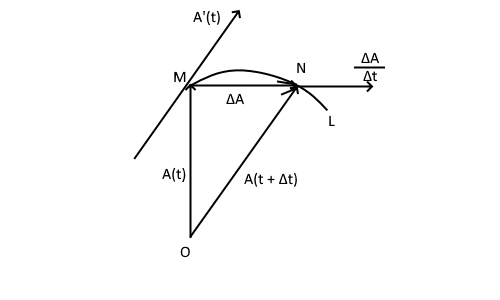
\includegraphics{resources/derivativeOfVectorFunction.png}

      即 : 矢径长度随时间的变化率
    }%矢量函数的导数

    \subsubsection{矢量函数的微分}{
      称$dA(t) = A\derivative(t)dt\ (\Delta t = dt)$为$A(t)$在$t$处的微分.在直角坐标系中有:

      $\cfrac{d\vec{A}}{dt} = A\derivative_x(t)\vec{i} + A\derivative_y(t)\vec{j} + A\derivative_z(t)\vec{k}$

      即 :

      $d\vec{A} = dA_x(t)\vec{i} + dA_y(t)\vec{j} + dA_z(t)\vec{k} = (A\derivative_x(t)\vec{i} + A\derivative_y(t)\vec{j} + A\derivative_z(t)\vec{k})dt$
    }%矢量函数的微分结尾

    \subsubsection{矢量函数的不定积分}{
      若$A\derivative(t) = a(t)$,则称$A(t)$是$a(t)$的原函数.$a(t)$的原函数的一般形式叫做$a(t)$的不定积分,记作 :

      $\int a(t)dt$

      若$A\derivative(t)$是$a(t)$的一个原函数,则有 :

      $\int a(t)dt = A(t) + \vec{\mathConstant}$\qquad ($\vec{\mathConstant}$为任意常矢)
    }

    \subsubsection{矢量函数的定积分}{
      类似于数性函数,$a(t)$在$[t_1,t_2]$上的定积分的定义为($A(t)\mbox{是}a(t)$的原函数) :

      $\definiteIntegral{t_2}{t_1}a(t)dt = \limNormal{n \to \infty}\limNormal{\lambda \to 0}\upDownSum{n}{i = 1}a(\xi_i)\Delta t_i$

      若$A(t)$是$a(t)$的一个原函数,则有 :
      $$
        \definiteIntegral{t_2}{t_1}a(t)dt = A(t_2) - A(t_1)\qquad \mbox{(微积分基本定理)}
      $$
      在直角坐标系中可分解为 :
      $$
        \definiteIntegral{t_2}{t_1}a(t)dt = \definiteIntegral{t_2}{t_1}a_x(t)dt\vec{i} + \definiteIntegral{t_2}{t_1}a_y(t)dt\vec{j} + \definiteIntegral{t_2}{t_1}a_z(t)dt\vec{k}
      $$
    }%矢量函数的定积分

    \begin{itemize}
      \item 从上述内容看出,矢量函数的微积分与数学分析(高等数学)中的微积分相类似,不过矢量函数要复杂些,他在直角坐标系中分解成三个数性函数,即他的三个分量.对矢量函数进行某一种运算,也就等于对他的各个分量进行这种运算.
      \item 矢量分解与坐标选取有关.在不同的坐标系中,有不同的表现形式,有的可能复杂的多.这里主要讨论直角坐标系的分解问题,多数问题还是会用分量表示.
    \end{itemize}

  }%场论基本内容结尾

  \subsection{场的分类与表示法}{

    \subsubsection{场的概念}{
      某一物理量在空间的分布就称为"场".在这个空间发生了物理现象,也就有物理量在这个空间分布.
    }%场的概念结尾

    \subsubsection{场的分类与表示}{
      场中每一点$M:(x,y,z)$都对应着一个物理量,即某个函数$\defFunction{M}$,如果这个函数是数量值函数,这种场就叫做数量场.如果是向量值函数,那么这种场就叫做矢量场.

      场中的物理量往往与点的位置有关,而且还将随时间变化.会随时间变化的场就叫做不稳定场(或不定常场),表示为 :
      $$
        u= \defFunction{M,t},\vec{A} = A(M,t)
      $$
      在三维直角坐标系(可推广至任意维)下也可分解为 :
      $$
        u = \defFunction{x,y,z,t}
      $$
      $$
        \vec{A} = A(x,y,z,t) = A_x(x,y,z,t)\vec{i} + A_y(x,y,z,t)\vec{j} + A_z(x,y,z,t)\vec{k}
      $$\spaceline

      如果场中物理量不随时间变换,这种场叫做稳定场(定常场),表示为 :
      $$
        u= \defFunction{M}\qquad \vec{A} = A(M)
      $$
      在三维直角坐标系(可推广)下也可以分解为 :
      $$
        u= \defFunction{x,y,z}
      $$
      $$
        \vec{A} = A(x,y,z) = A_x(x,y,z)\vec{i} + A_y(x,y,z)\vec{j} + A_z(x,y,z)\vec{k}
      $$
      在不稳定场中,美以固定时刻也就是稳定场.在场论中,讨论稳定场是基础.对于不稳定场,可以在讨论不稳定场的基础上再讨论对时间的变化.因此接下来一大段着重讨论稳定场的规律.
    }%场的分类与表示

    \subsubsection{场的直观表示}{
      在数量场中,物理量是点的坐标$(x,y,z)$的函数 :
      $$
        u = \defFunction{x,y,z}
      $$
      当u为某常数$\mathConstant$时,所有满足$\defFunction{x,y,z} = \mathConstant$的点就组成一个曲面.这个曲面的特点是在其上的点$(x,y,z)$处的函数值$u$相等,即
      $$
        \defFunction{x,y,z} = \mathConstant
      $$
      此曲面称为等值面,在平面中也被称为等值线.

      在矢量场中用矢量线表示.场中的曲线$L$,若他每点的切线方向与场在该点的矢量方向平行,则$L$称为该矢量场的矢量线.矢量线满足微分方程 :
      $$
        \cfrac{dx}{A_x} = \cfrac{dy}{A_y} = \cfrac{dz}{A_z}
      $$

      \begin{itemize}
        \item 矢量线$L$不止有一个,而是一族曲线.矢量线$L$存在于场中,$L$上每一点都有一个矢量$\vec{A} = \begin{bmatrix}
                  A_x & A_y & A_z
                \end{bmatrix}$
        \item 矢量线$L$只反映矢量场在$L$上每点的方向,并没有大小数量关系.
        \item 等值面(线)是满足等函数值的自变量全体.因为C时任意常数,所以$\defFunction{x,y,z} = \mathConstant$表示等值面族.
      \end{itemize}
    }%场的直观表示结尾

  }%场的分类与表示法结尾

  \subsection{方向导数与梯度}{

    \subsubsection{方向导数的定义}{
      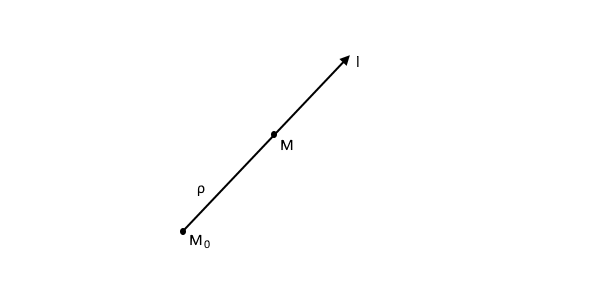
\includegraphics{resources/directionDerivative1.png}

      从数量场$u= u(M)$中任一点$M_0$出发引一条有向射线$\vec{l}$,在$\vec{l}$上任取一点$M$,记$\vec{M_0M} = \rho$,当沿$\vec{l}$,$M \to M_0$时,此式的极限存在 :
      $$
        \cfrac{\Delta u}{\vec{\rho}} = \cfrac{u(M) - u(M_0)}{\vec{M_0M}}
      $$
      称此极限值为函数$u(M)$在点$M_0$处沿方向$\vec{l}$的方向导数,记为$\directionDerivative{u}{l}{M_0}$,即 :
      $$
        \directionDerivative{u}{l}{M_0} = \limNormal{M \to M_0}\cfrac{u(M) - u(M_0)}{M_0M}
      $$

      \begin{itemize}
        \item 方向导数是一个数量,他与点$M_0$有关,也与方向$\vec{l}$有关.
        \item {
              以平面数量场为例说明方向导数的意义 :

              设数量场
              $$
                u = \defFunction{x,y}
              $$
              不难看出 :
              % #TODO 画图
              $$
                \cfrac{\Delta u}{\rho} = \cfrac{u(M) - u(M_0)}{\vec{M_0M}} = \cfrac{\defFunction{M} - \defFunction{M_0}}{\vec{M_0M}}
              $$
              正是沿着$\vec{l}$方向,函数$\defFunction{x,y}$从点$M_0$到点$M$的平均升高,即平均变化率.而极限 :
              $$
                \limNormal{M \to M_0}\cfrac{\Delta u}{\vec{\rho}} = \limNormal{M \to M_0}\cfrac{\defFunction{M} - \defFunction{M_0}}{\vec{M_0M}} (\mbox{沿着})\vec{l}
              $$
              是$u = \defFunction{x,y}$在点$M_0$沿$\vec{l}$的变化率.所以方向导数是变化率,它反映了函数$u = \defFunction{x,y}$在$\vec{l}$方向上的增减情况.当$\directionDerivative{u}{l}{M_0} > 0$,表示函数$u = \defFunction{x,y}$在点$M_0$沿方向$\vec{l}$是增加的,越大表示增加的越快,反之亦然.
              }
        \item 偏导数是方向导数的特例.比如当$\vec{l}$指向x轴正向时,$\cfrac{\partial u}{\partial l} = \cfrac{\partial u}{\partial x}$,当$\vec{l}$指向y轴正向时,$\cfrac{\partial u}{\partial l} = \cfrac{\partial u}{\partial y}$.
        \item 有时候要考虑函数沿某曲线C的导数.函数沿曲线C的每一点的切线方向的方向导数叫做函数沿曲线C的导数.
      \end{itemize}
    }%方向导数的定义结尾

    \subsubsection{方向导数的计算公式}{
      设$u= u(x,y,z)$在$M_0(x_0,y_0,z_0)$处可微,$\vec{l}$的方向余弦是$\cos\alpha,\cos\beta,\cos\gamma$,则u在点$M_0$沿$\vec{l}$的方向导数为 :
      $$
        \directionDerivative{u}{l}{M_0} = \directionDerivative{u}{x}{M_0}\cos\alpha + \directionDerivative{u}{y}{M_0}\cos\beta + \directionDerivative{u}{z}{M_0}\cos\gamma
      $$
      或者 :
      $$
        \directionDerivative{u}{l}{M_0} = \partialDerivativeFrac{u}{x}\cos\alpha + \partialDerivativeFrac{u}{y}\cos\beta + \partialDerivativeFrac{u}{z}\cos\gamma
      $$
    }%方向导数的计算公式结尾    

    \subsubsection{梯度}{
      设数量场$u = u(M)$,如果在���中任一点$M$处,存在非零矢量$\vec{G}$,其方向为函数$u(M)$在$M$点处方向导数的最大的方向,其模$|\vec{G}|$这个最大的方向导数值,则称矢量$\vec{G}$为数量场$u$在点$M$处的梯度,记为 :
      $$
        \gradText u = \vec{G}
      $$
      在直角坐标系中有 :
      $$
        \gradText u = \begin{bmatrix}
          \partialDerivativeFrac{u}{x} & \partialDerivativeFrac{u}{y} & \partialDerivativeFrac{u}{z}
        \end{bmatrix} = \partialDerivativeFrac{u}{x}\vec{i} + \partialDerivativeFrac{u}{y}\vec{j} + \partialDerivativeFrac{u}{z}\vec{k}
      $$

      引入$grad\ u = \triangledown u$

      \begin{itemize}
        \item 梯度是刻划数量场的概念.数量场的梯度是一个矢量.
        \item 任一点的梯度垂直于过该点的等值面(线),并且指向$u(M)$增大的一方.因而梯度方向平行于等值面(线)的法线方向.
        \item 数量场的每一点都有一个梯度,他是矢量,数量场的梯度场是矢量场,称为$u(M)$的梯度场.
        \item $\partialDerivativeFrac{u}{l} = \nabla u \cdot l_0$,其中$l_0= \cfrac{l}{|l|}$
        \item $\nabla$称为nabla算子
      \end{itemize}
    }%梯度结尾

    \subsubsection{梯度的运算公式}{
      \begin{itemize}
        \item $\gradText \mathConstant = 0$
        \item $\gradText (\mathConstant u) = \mathConstant \triangledown u$
        \item $\gradText (u \pm v) = \triangledown u + \triangledown v$
        \item $\gradText (uv) = v\triangledown u + u\triangledown v$
        \item $\gradText (\cfrac{u}{v}) = \cfrac{v\triangledown u - u\triangledown v}{v^2}\qquad (v \neq 0)$(注意:与导数的顺序不同)
        \item $\gradText \defFunction{u} = \fDerivative{u}\triangledown u$
        \item 以上的公式都可以改写成用$\nabla$算子的形式
      \end{itemize}
    }%梯度的运算公式

  }%方向导数与梯度结尾

  \subsection{通量与散度,高斯公式}{
    对于一个矢量场,主要讨论他的两个基本性质 : 其一是有没有源,其二是有没有旋

    \subsubsection{通量}{
      定义 : 设矢量场$A(M)$,将沿着场中某一有向曲面$S$的曲面积分 :
      $$
        \varPhi = \doubleIntegralOnZone{S} A_n dS = \doubleIntegralOnZone{s} A \cdot d\mathbf{S}
      $$
      称为矢量场$A(M)$向正侧穿过曲面$S$的通量.其中$d\mathbf{S} = \vec{n}dS$,$\vec{n}$是$dS$的法线方向,$A_n = A \cdot \vec{n}$

      说明 :
      \begin{itemize}
        \item {通量$\varPhi$是一个数量.(顾名思义,通量就是矢量$\vec{A}$通过$S$的量,$A$可以表示流速,电场,磁场的强度等.相应的$\varPhi$就是流量,电通量,磁通量等.)因为$d\mathbf{S} = \vec{n}dS$,$A\cdot d\mathbf{S}$有正负之分

              \begin{itemize}
                \item $\vecAngle{\vec{A}}{\vec{n}} < \cfrac{\pi}{2},\varPhi > 0$
                \item $\vecAngle{\vec{A}}{\vec{n}} > \cfrac{\pi}{2},\varPhi < 0$
                \item $\vec{A} \perp \vec{n},\varPhi = 0$.
              \end{itemize}

              在一个矢量场中,每点上的$\vec{A}$是确定对.$\varPhi$的正负与$\vec{n}$的制定有关.
              }
        \item {
              若$S$是闭曲面,一般去向外法线方向为正向.因此 :

              \begin{itemize}
                \item $\varPhi > 0$,表示$S$内部有源.这意味着穿过$S$流入的量小于流出的量,而$\varPhi$正是流出量与流入量的差,因此$S$内部有源.$\varPhi$就是由$S$散发出去的量.
                \item $\varPhi < 0$,表示$S$内部有洞.流出的量小于流入的量,$\varPhi$就是流入的多余部分,���个量再$S$所包围的区域内被吸收或者渗掉,所以有洞.$\varPhi$是吸收入$S$内部的量.
                \item $\varPhi = 0$,说明流入等于流出.
              \end{itemize}
              }
        \item {
              由定义得 :
              $$
                d\varPhi = \vec{A} \cdot d\mathbf{S}
              $$

              表示流过面积元$dS$的正向的通量.
              }
      \end{itemize}
    }%通量结尾

    \subsubsection{散度}{
      通量描述了一固定区域上向量场的流通倾向,而散度在某点的的值则是这个性质在这点的局部描述,也就是说,从散度在一点的值,就可以看出向量场在这点附近到底是倾向于发散还是收敛.

      设��量场$A(M)$,在场中作包围点$M$的闭曲面$S$,$S$包围的趋于称为$\Omega$,$\Omega$的体积为$\Delta V$.当$\Omega$收缩到极限$M$时,如果极限 :
      $$
        \limNormal{\Omega \to M}\cfrac{\doubleCurveIntegralOnZone{S}A \cdot d\mathbf{S}}{\Delta V}
      $$
      存在,则称此极限值为向量场$A$在点$M$处的散度.记为$\divergenceText A$,即 :
      $$
        \divergenceText A = \limNormal{\Omega \to M}\cfrac{\doubleCurveIntegralOnZone{S}A \cdot d\mathbf{S}}{\Delta V}
      $$

      说明 :
      \begin{itemize}
        \item {
              散度是刻画矢量场的基本性质的量,是数量.$\divergenceText A$形成一个数量场,称为矢量场$A$的散度场.
              }
        \item {
              散度,顾名思义就是向量场一点处发散量的大小.在$M$点 :
              \begin{itemize}
                \item $\divergenceText A > 0$,表示M点有源.值越大,表示源$M$的发散量越大.
                \item $\divergenceText A < 0$,表示M点有洞.绝对值越大,表示这个洞吸收量越大(或渗的越快).
                \item $\divergenceText A = 0$,表示$M$点无源无洞.
              \end{itemize}
              }
        \item {
              由定义可知,$\divergenceText A$就是单位体积的通量的极限,也就是通量的密度.
              }
        \item {
              散度算子为$\divergenceSymbol$,表示点乘结果为数.
              }
        \item {
              还有一种理解方法 : 散度表示当$x,y,z$有微小增加时,向量场分量增加量的总和.散度在各个方向是一样的,不随坐标系旋转而改变.
              }
      \end{itemize}
    }%散度

    \subsubsection{散度在常见坐标系中的计算公式}{
      在不同的坐标系下,向量场的散度有不同的表达方. :
      \begin{itemize}
        \item {
              直角坐标系 :

              在三维直角坐标系$xyz$中,设向量场$A$的表示为 :
              $$
                A(x,y,z) = A_x(x,y,z)\vec{i} + A_y(x,y,z)\vec{j} + A_z(x,y,z)\vec{k}
              $$

              其中$\vec{i},\vec{j},\vec{k}$分别是$x,y,z$轴上的单位向量,场的分量$A_x,A_y,A_z$具有一阶连续偏导数,那么向量场$A$的散度就是 :
              $$
                \divergenceText A = \divergenceSymbol A = \partialDerivativeFrac{A_x}{x} + \partialDerivativeFrac{A_y}{y} + \partialDerivativeFrac{A_z}{z}
              $$
              }
        \item {
              圆柱坐标系 :

              圆柱坐标系中,假设物体的位置为$(\rho,\varphi,z)$,定义其径向单位矢量,横向单位的矢量和纵向单位的矢量为

              $\vec{e_{\rho}},\vec{e_{\varPhi}},\vec{e_z}$,那么向量场$A$可以表示为 :
              $$
                A = A_{\rho}(\rho,\varphi,z)\vec{e_{\rho}} + A_{\varphi}(\rho,\varphi,z)\vec{e_{\varphi}} + A_{z}(\rho,\varphi,z)\vec{e_{z}}
              $$
              向量场$A$的散度就是 :
              $$
                \divergenceText A = \divergenceSymbol A = \cfrac{1}{\rho}\partialDerivativeFrac{\rho A_\rho}{\rho} + \cfrac{1}{\rho}\partialDerivativeFrac{A_\varphi}{\varphi} + \partialDerivativeFrac{A_z}{z}
              $$
              }
        \item {
              球坐标系 :

              球坐标系中,假设物体的位置用球坐标系表示为$(r,\theta,\varphi)$,定义它的基向量 : $\vec{e_r},\vec{e_\theta},\vec{e_\varphi}$,则向量场$A$可以表示为 :
              $$
                A = A_r(r,\theta,\varphi)\vec{e_r} + A_\theta(r,\theta,\varphi)\vec{e_\theta} + A_\varphi(r,\theta,\varphi)\vec{e_\varphi}
              $$
              向量场$A$的散度就是 :
              $$
                \divergenceText A = \divergenceSymbol A = \cfrac{1}{r^2}\partialDerivativeFrac{r^2A_r}{r} + \cfrac{1}{r\sin\theta}\partialDerivativeFrac{\sin\theta A_\theta}{\theta} + \cfrac{1}{r\sin\theta}\partialDerivativeFrac{A_\varphi}{\varphi}
              $$
              }
      \end{itemize}
    }%散度在常见坐标系中的计算公式

    \subsubsection{高斯散度定理/高斯公式/高斯-奥斯特洛格拉特斯基公式}{
      既然向量场某一处的散度是向量场在该处附近通量的体密度,那么对某一个体积内的散度进行积分,就应该得到这个体积内的总通量.事实上可以证明这个推论是正确的,称为高斯散度定理.高斯定理说明,如果在体积V内的向量场A拥有散度,那么散度的体积分等于向量场在V的表面S的面积分

      设矢量场$A = P\vec{i} + Q\vec{j} + R\vec{k}$的各分量$P,Q,R$再闭曲面所围区域$\Omega$内有一阶连续偏导数,则有 :
      $$
        \doubleCurveIntegralOnZone{S}A \cdot d\mathbf{S} = \tripleIntegralOnZone{\Omega}\divergenceText AdxdydZ
      $$
      或者 :
      $$
        \doubleCurveIntegralOnZone{S}Pdydz + Qdzdx + Rdxdy = \tripleIntegralOnZone{\Omega}\left(\partialDerivativeFrac{P}{x} + \partialDerivativeFrac{Q}{y} + \partialDerivativeFrac{R}{z}\right)dxdydz
      $$

      说明 :
      \begin{itemize}
        \item {
              高斯公式是重要公式,它的意义是曲面积分与体积分互化.因为曲面积分不易计算,所以将曲面积分化作了三重积分
              }
        \item {
              高斯公式的物理意义是 : 矢量场通过任意闭曲面$S$的通量等于他所包围的体积$V$内散度的总和.
              }
      \end{itemize}
    }%高斯散度定理/高斯公式/高斯-奥斯特洛格拉特斯基公式结尾

    \subsubsection{散度的运算性质}{
      \begin{itemize}
        \item {
              由于散度是线性算符,所以 :
              $$
                \divergenceSymbol(aF \pm bG) = a\divergenceSymbol F \pm b\divergenceSymbol G
              $$
              其中$F,G$是向量场,$a,b$是实数.
              }
        \item {
              $\divergenceSymbol(\varphi A) = grad \varphi \cdot A + \varphi\divergenceSymbol A$

              其中$\varphi$是数性函数.
              }
        \item {
              $\divergenceSymbol (\vec{\mathConstant}\varphi) = \vec{\mathConstant} \cdot grad \varphi$
              }
      \end{itemize}

      注意 :
      \begin{itemize}
        \item 散度是对矢量场而言的,所以对一个标量函数求散度无意义.
        \item {
              散度运算与通常的微分运算相似 :
              $$
                d(uv) = vdu + udv
              $$
              若是直接仿照应当有$\divergenceSymbol (\varphi A) = \varphi\divergenceSymbol A + A\divergenceSymbol \varphi$,但是由于$\varphi$是数性函数,求散度无意义,只有写成$grad \varphi$才有意义.于是就能满足散度是一个"数量"的要求.
              }
      \end{itemize}
    }%散度的运算性质

  }%通量与旋度,高斯公式

  \subsection{环量,旋度,斯托克斯公式}{
    \subsubsection{环量}{
      设矢量场$A(M)$,将沿着场中某一有向封闭曲线$l$的曲线积分 : $$
        \Gamma = \curveIntegralOnLine{l}A \cdot dl
      $$

      称为矢量场$A$按照所取方向沿着曲线$l$的环量.

      说明 :
      \begin{itemize}
        \item 环量与通量一样,是一个刻画矢量场的特征量.
        \item 环量是一个数量,他的数值除了与场$A$有关外,还和回路$l$的形状和取向有关,说明$\Gamma$并不只是表示向量场本身内在属性的量,为了只表示场$A$本身的性质,就需要让$l$收缩到一点,为此引入环量面密度.
      \end{itemize}
      %#TODO wiki
    }%环量结尾

    \subsubsection{环量面密度}{
      设$M$是矢量场中的一点,在$M$点取一矢量$\vec{n}$,并且在$M$点附近取回路$l$,作以$l$为边界,$\vec{n}$为法线且过$M$的曲面$\Delta S$,并取$l$的正向与$n$构成右手系.令$l$沿着$\Delta S$以任意方式收缩到$M$点,如果极限$$
        \limNormal{l \to M(\mbox{沿着}\Delta S)}\cfrac{\curveIntegralOnLine{l}A \cdot dl}{\Delta S}
      $$
      存在,则称此极限值为向量场$A$在点$M$处沿方向$\vec{n}$的环量面密度.记为$L_{n}$

      说明 :
      \begin{itemize}
        \item $L_n$是单位面积的环量的极限.在物理上,单位面积的某个两被称为面密度.$\cfrac{\curveIntegralOnLine{l}A \cdot dl}{\Delta S}$是平均单位面积的环量,即$\Delta S$上的平均面密度.用微分方法处理,取极限得到了在$M$点的环量密度,与$l$的形状无关.
        \item $L_n$的大小反映了在点$M$沿着$\vec{n}$方向的旋转强弱情况.
        \item $L_n$的大小与取定的方向$\vec{n}$有关.在空间中一点,方向$L_n$可以任取,于是又无穷多个$L_n$,这些$L_n$中有一个最大者,沿着最大者的方向,场在该点旋转最强,于是引入旋度概念.
      \end{itemize}
    }%环量面密度结尾

    \subsubsection{旋度}{
      若在向量场$A$中的一点$M$处存在矢量$\vec{R}$,他的方向是$A$在该点环量面密度最大的方向,他的模就是这个最大的环量面密度.矢量$\vec{R}$称为向量场$A$在点$M$的旋度,记为$\curlRotText A$或者$\curlText A$

      说明 :
      \begin{itemize}
        \item 旋度是刻划向量场的一个特征量.说明一个矢量场是否有旋以及旋转强弱.
        \item 旋度与环量中$l$的形状,取向都无关,只与场在$M$点的量$A(M)$本身有关,他是代表矢量场本身内在属性的量.
        \item 旋度是一个向量算子,表示在三维欧几里得空间中的向量场的无穷小量旋转.在向量场的每个点上,点的旋度表示为一个向量,称为旋度向量.这个向量的模和方向刻画了在这个点上的强度和旋转方向.
        \item 由定义知旋度与环量面密度的关系 : $L_n = \curlRotText A \cdot \vec{n}$
        \item 旋转的方向是旋转的轴,它由右手定则来确定,而旋度的大小是旋转的量.如果向量场表示一个移动的流形的流速,则旋度是这个流形的环量面密度.旋度为0的向量场叫做无旋向量场.旋度是向量的一种微分形式.微积分基本定理的对应形式是开尔文-斯托克斯定理(斯托克斯公式),他将向量场旋度的曲面积分关联到这个向量场环绕的边界曲线的曲线积分.
        \item 不同于梯度和散度,旋度不能简单的推广到其他维度;某些推广是可能的,但是只有在三位中,在几何上定义的向量场旋度还是向量场.这个现象类似于三维叉积,此联系反映在了旋度的符号$\curlSymbol$上.
        \item 矢量场每点都对应一个旋度,这些旋度就形成了一个新的矢量场,称为原矢量场$A$的旋度场$\curlRotText A$.
      \end{itemize}
    }%旋度结尾

    \subsubsection{旋度在直角坐标系中的运算公式}{
      设矢量场$A$ : $$
        A = P(x,y,z)\vec{i} + Q(x,y,z)\vec{j} + R(x,y,z)\vec{k}
      $$
      且$P,Q,R$具有一阶连续偏导数,则 : $$
        \curlRotText A = \bigCase{\partialDerivativeFrac{R}{y} - \partialDerivativeFrac{Q}{z}}\vec{i} + \bigCase{\partialDerivativeFrac{P}{z} - \partialDerivativeFrac{R}{x}}\vec{j} + \bigCase{\partialDerivativeFrac{Q}{x} - \partialDerivativeFrac{P}{y}}\vec{k}
      $$
      可以写成便于记忆的行列式(只是便于记忆,只有形式上的意义,无实际意义) : $$
        \curlRotText A = \begin{vmatrix}
          \vec{i}                       & \vec{j}                       & \vec{k}                       \\
          \partialDerivativeFrac{\ }{x} & \partialDerivativeFrac{\ }{y} & \partialDerivativeFrac{\ }{z} \\
          P                             & Q                             & R
        \end{vmatrix}
      $$
    }%旋度在直角坐标系中的运算公式结尾

    \subsubsection{旋度的运算性质}{
      \begin{itemize}
        \item $\curlRotText (\vec{A} \pm \vec{B}) = \curlRotText \vec{A} \pm \curlRotText \vec{B}$
        \item $\curlRotText (\varphi \vec{A}) = \varphi \curlRotText \vec{A} + \gradText \varphi \times \vec{A}$($\varphi$是数性函数)
        \item $\curlRotText \mathConstant \vec{A} = \mathConstant \curlRotText \vec{A}$
        \item $\curlRotText (\varphi \vec{a}) = \gradText \varphi \times \vec{a}$($\vec{a}$为常向量)
      \end{itemize}
    }%旋度的运算性质结尾

    \subsubsection{斯托克斯公式}{
      设矢量场$A = P\vec{i} + Q\vec{j} + R\vec{k}$的分量$P,Q,R$在包围曲面$S$的空间区域中有一阶连续偏导数,$l$为曲面$S$的边界,则 : $$
        \curveIntegralOnLine{l}A \cdot dl = \surfaceIntegralOnSurface{S}\curlRotText A\cdot dS
      $$
      或者写成 : $$
        \curveIntegralOnLine{l}Pdx + Qdy + Rdz = \surfaceIntegralOnSurface{S}\mediumBigCase{\bigCase{\partialDerivativeFrac{R}{y} - \partialDerivativeFrac{Q}{z}}dydz + \bigCase{\partialDerivativeFrac{P}{z} - \partialDerivativeFrac{R}{x}}dzdx + \bigCase{\partialDerivativeFrac{Q}{x} - \partialDerivativeFrac{P}{y}}dxdy}
      $$

      说明 :
      \begin{itemize}
        \item 斯托克斯公式也是重要公式之一,利用它可以把曲线积分转换为曲面积分,或者相反.
        \item 由于计算曲面积分困难,而曲线积分可以直接计算,若用斯托克斯公式化为曲面积分,除了特殊情况外可能会更难计算,因此斯托克斯公式没有高斯公式用的多.
        \item 此公式的意义就是向量场在任意闭回路$l$上的环量等于以$l$为边界的曲面$S$上的旋度的总和.
        \item 注意 : 高斯公式把闭曲面的曲面积分华为三重积分,斯托克斯则把曲线积分华为以$l$为边界的曲面积分,如果不能化为闭曲面的曲面积分,也就不能化成三重积分.
      \end{itemize}

      当$A$为平面向量场是,斯托克斯公式会变成格林公式,斯托克斯公式可以看作是格林公式的推广.
    }%斯托克斯公式

  }%环量,旋度,斯托克斯公式结尾

  \subsection{几个特殊的向量场}{

    \subsubsection{管形场}{
      在向量场$A$中,如果$\divergenceText A = 0$,则称$A$为管形场,又称无源场.

      管形场的判别法 : A为管形场$\Leftrightarrow \divergenceText A = 0$.

      管形场的一条重要性质就是 : 场中任一矢量管(由矢量线所组成的管型曲面)的所有横截面的通量都相等.
    }%管形场结尾

    \subsubsection{有势场}{
      在矢量场$A(M)$中,如果存在函数$u(M)$使得$A = \gradText u$,则称$A$为有势场.称$v = -u$为矢量场$A$的势函数.

      有以下等价定义 :
      \begin{itemize}
        \item $A = P\vec{i} + Q\vec{j} + R\vec{k}$为有势场
        \item $\curlRotText A = 0$
        \item $\curveIntegralOnLine{l} A \cdot dl = 0$($l$为任意闭曲线)
        \item $\definiteIntegral{M}{M_0}A \cdot dl$与路径无关.
        \item 存在函数$u$使得$du(x,y,z) = Pdx + Qdy + Rdz$
      \end{itemize}
      以上五条定义都互相等价

      有势场的判别方法 : 如果$\curlRotText A = 0$,则$A$为有势场.

      使用这一判别方法比较方便,当然等价定义也可以用于判别.\spaceline

      求势函数的方法 :
      \begin{enumerate}
        \item {
              公式法 :

              任取一点$M_0(x_0,y_0,z_0)$,则$$
                u(x,y,z) = \definiteIntegral{x}{x_0}P(x,y_0,z_0)dx + \definiteIntegral{y}{y_0}Q(x,y,z)dy + \definiteIntegral{z}{z_0}R(x,y,z)dz %# TODO 查错
              $$
              则势函数$v(x,y,z) = -u(x,y,z)$
              }
        \item {
              凑全微分法 :

              找一个函数$u(x,y,z)$,使得$$
                du = Pdx + Qdy + Rdz
              $$
              则势函数$v(x,y,z) = -u(x,y,z)$
              }
        \item 积分法:微分法换一种思路,解微分方程.
      \end{enumerate}
    }%有势场结尾

    \subsubsection{调和场}{
      矢量场$A$中,若$\divergenceText A = 0$且$\curlRotText A = 0$,则称$A$是调和场.也叫做无源无旋场.

      说明 :
      \begin{itemize}
        \item 调和场$\Leftrightarrow$有势场且管形场
        \item {
              调和场是有势场,必有$u$存在,使$$
                \gradText u = A
              $$
              又因为是管形场,所以$\divergenceText A = \divergenceText\gradText u = 0$,即$\Delta u = 0$(参考公式表)

              $u$称为调和场的调和函数.
              }
      \end{itemize}
    }%调和场结尾

  }%几个特殊的向量场结尾

  \subsection{nabla算子(哈密尔顿算子)}{

    \subsubsection{定义}{
      $$
        \nabla = \vec{i}\partialDerivativeFrac{\ }{x} + \vec{j}\partialDerivativeFrac{\ }{y} + \vec{k}\partialDerivativeFrac{\ }{z} = \begin{Bmatrix}
          \partialDerivativeFrac{\ }{x} & \partialDerivativeFrac{\ }{y} & \partialDerivativeFrac{\ }{z}
        \end{Bmatrix}
      $$
      称为哈密尔顿算子(nabla算子).它是一个向量形式的微分算子,兼有微分运算和向量运算的双重作用.它本身既不是一个函数也不是某个物理量.他表示的是一种运算,以一定方式作用于函数式向量后才能表示一个量.
    }%nabla算子定义结尾

    \subsubsection{运算规则}{
      \begin{itemize}
        \item $\nabla u = \bigCase{\vec{i}\partialDerivativeFrac{\ }{x} + \vec{j}\partialDerivativeFrac{\ }{y} + \vec{k}\partialDerivativeFrac{\ }{z}}u = \partialDerivativeFrac{u}{x}\vec{i} + \partialDerivativeFrac{u}{y}\vec{j} + \partialDerivativeFrac{u}{z}\vec{k} = \begin{bmatrix}
                  \partialDerivativeFrac{u}{x} & \partialDerivativeFrac{u}{y} & \partialDerivativeFrac{u}{z}
                \end{bmatrix}$
        \item $\divergenceSymbol A = \bigCase{\vec{i}\partialDerivativeFrac{\ }{x} + \vec{j}\partialDerivativeFrac{\ }{y} + \vec{k}\partialDerivativeFrac{\ }{z}} \cdot (P\vec{i} + Q\vec{j} + R\vec{k}) = \partialDerivativeFrac{P}{x} + \partialDerivativeFrac{Q}{y} + \partialDerivativeFrac{R}{z}$
        \item $\curlSymbol A = \bigCase{\vec{i}\partialDerivativeFrac{\ }{x} + \vec{j}\partialDerivativeFrac{\ }{y} + \vec{k}\partialDerivativeFrac{\ }{z}} \times (\vec{i}P + \vec{j}Q + \vec{k}R) = \begin{vmatrix}
                  \vec{i}                       & \vec{j}                       & \vec{k}                       \\
                  \partialDerivativeFrac{\ }{x} & \partialDerivativeFrac{\ }{y} & \partialDerivativeFrac{\ }{z} \\
                  P                             & Q                             & R
                \end{vmatrix}\\
                = \vec{i}\bigCase{\partialDerivativeFrac{R}{y} - \partialDerivativeFrac{Q}{z}} + \vec{j}\bigCase{\partialDerivativeFrac{P}{z} - \partialDerivativeFrac{R}{x}} + \vec{k}\bigCase{\partialDerivativeFrac{Q}{x} - \partialDerivativeFrac{P}{y}}$
      \end{itemize}

      说明 :
      \begin{itemize}
        \item {
              $\nabla$算子可以作用到数性函数,也可以作用到向量函数,有三种形式 : $$
                \nabla u \quad \divergenceSymbol A \quad \curlSymbol A
              $$
              }
        \item {
              $\nabla$不是向量,所以$A \cdot \nabla \neq \divergenceSymbol A$ :

              $$
                \divergenceSymbol A = \partialDerivativeFrac{\ }{x}A_x + \partialDerivativeFrac{\ }{y}A_y + \partialDerivativeFrac{\ }{z}A_z
              $$

              $$
                A \cdot \nabla = A_x\partialDerivativeFrac{\ }{x} + A_y\partialDerivativeFrac{\ }{y} + A_z\partialDerivativeFrac{\ }{z}
              $$
              }
      \end{itemize}
    }%运算规则结尾

    \subsubsection{梯度散度旋度以及高斯公式和斯托克斯公式的算子表示法}{
      梯度 : $\nabla u = \gradText u$

      散度 : $\divergenceSymbol A = \divergenceText A$

      旋度 : $\curlSymbol A = \curlRotText A$

      高斯公式 : $\doubleCurveIntegralOnZone{S} A \cdot d\mathbf{S} = \tripleIntegralOnZone{\Omega} \divergenceSymbol A d\Omega$

      斯托克斯公式 : $\curveIntegralOnLine{l} A \cdot dl = \surfaceIntegralOnSurface{S}\curlSymbol A \cdot ds$
    }%梯度散度旋度以及高斯公式和斯托克斯公式的算子表示法

    \subsubsection{常用公式}{
      \begin{itemize}
        \item $\nabla(\mathConstant u) = \mathConstant \nabla u$
        \item $\divergenceSymbol(\mathConstant\vec{A}) = \mathConstant \divergenceSymbol \vec{A}$
        \item $\curlSymbol(\mathConstant \vec{A}) = \mathConstant \curlSymbol \vec{A}$
        \item $\nabla(u \pm v) = \nabla u \pm \nabla v$
        \item $\divergenceSymbol(\vec{A} \pm \vec{B}) = \divergenceSymbol \vec{A} \pm \divergenceSymbol \vec{B}$
        \item $\curlSymbol(\vec{A} \pm \vec{B}) = \curlSymbol\vec{A} \pm \curlSymbol\vec{B}$
        \item $\divergenceSymbol(u\vec{\mathConstant}) = \nabla u \cdot \vec{\mathConstant}$
        \item $\curlSymbol(u\vec{\mathConstant}) = \nabla u \times \vec{\mathConstant}$
        \item $\nabla(uv) = u\nabla v + v\nabla u$
        \item $\divergenceSymbol(u\vec{A}) = \nabla u \cdot \vec{A} + u \divergenceSymbol \vec{A}$
        \item $\curlSymbol(u\vec{A}) = \nabla u \times \vec{A} + u \curlSymbol \vec{A}$
        \item $\nabla(\vec{A} \cdot \vec{B}) = (\vec{A} \cdot \nabla)\vec{B} + (\vec{B} \cdot \nabla)\vec{A} + \vec{A}\times(\curlSymbol\vec{B}) + \vec{B}\times(\curlSymbol\vec{A})$
        \item $\divergenceSymbol(\vec{A}\times\vec{B}) = \vec{B}\cdot(\curlSymbol\vec{A}) - \vec{A}\cdot(\curlSymbol\vec{B})$
        \item $\curlSymbol(\vec{A} \times \vec{B}) = (\vec{B} \cdot \nabla)\vec{A} - (\vec{A} \cdot \nabla)\vec{B} + (\divergenceSymbol\vec{B})\vec{A} - (\divergenceSymbol\vec{A})\vec{B}$
        \item $\divergenceSymbol\nabla u = \nabla^2 u = \laplaceOperator u$($\laplaceOperator \equiv  \cfrac{\partial^2}{\partial x^2} + \cfrac{\partial^2}{\partial x^2} + \cfrac{\partial^2}{\partial z^2}$为拉普拉斯算符,$\laplaceOperator u$称为调和量)
        \item $\curlSymbol(\nabla u) = 0$(数量场的梯度场是无旋场)
        \item $\divergenceSymbol(\curlSymbol\vec{A}) = 0$(向量场的旋度场是无源场)
        \item $\curlSymbol(\curlSymbol\vec{A}) = \nabla(\divergenceSymbol\vec{A}) - \laplaceOperator\vec{A}$
      \end{itemize}
      $$
        \laplaceOperator \vec{A} = \laplaceOperator A_x\vec{i} + \laplaceOperator A_y\vec{j} + \laplaceOperator A_z\vec{k}
      $$
    }%常用公式结尾

  }%nabla算子结尾

  %#TODO 梯度,散度,旋度在不同坐标系中的表达式,整理,将A和B改写成\vec{f},\vec{g}此类形式,合并至多元微积分.

 }%场论结尾
  %*数学分析_2
  % \chapter{数学分析}{
\section{映射与函数}{

\subsection{映射}{
    映射指的是集合之间的一种对应关系.

    定义 : $X,Y$是两集合,按照某个规则$f$,对于任一的$x \in X$,有唯一的$y \in Y$与之对应,则称$f$是$X$到$Y$的一个映射.

    记为 : $f: X \to Y$,即 : $x \mapsto y = \defFunction{x}$

    称呼 :

    \begin{itemize}
        \item $y$ : 在映射$f$下,x的像.
        \item $x$ : 在映射$f$下,y的\textcolor{red}{一个}逆像.
        \item $X$ : $f$的定义域,记为$X = D_f$.
        \item $Y$ : $f$的值域,记为$R_f \subset Y$,具体的来说,$R_f = \set{y | y \in Y \land \exists x(y = f(x) \land x \in X)}$
    \end{itemize}

    举例 : 设$X$是平面上三角形的全体,$Y$是平面上圆的全体,构造一个映射$f$,表示(y 是 x 的外接圆),记为 : $$
        f : \underset{x \mapsto y}{X \to Y}
    $$

    \subsubsection{映射的基本要素}{
        \begin{itemize}
            \item $X = D_f$,定义域.
            \item $Y$,限制值域的范围.
            \item $f$,需要保证像的唯一性.
        \end{itemize}

        这说明了两点 : \begin{enumerate}
            \item {
                  映射的像是唯一的,举例 :

                  设$X = \mathRealNumberCollection^+ = \set{x | x \in R \land x > 0}$,假设存在映射$f : \underset{x \mapsto y}{X \to Y}(y^2 = x)$,此时$Y = \mathRealNumberCollection$,那么假设$x = 4,y = \pm 2$.这个映射就无法保证像的唯一性.换句话说,这个$f$并不是个映射.

                  但是可以稍作改造:对$Y = \mathRealNumberCollection$做限制,令$Y = R^-$,此时 : $$
                      \mapsToWithSubText{f}{X \to Y}{x \mapsto y}(y^2 = x)
                  $$
                  就构成了一个映射
                  }
            \item {
                  映射不要求逆向唯一.
                  }
        \end{enumerate}
    }%映射的基本要素结尾

    \subsubsection{映射的分类}{
        \begin{itemize}
            \item {
                  单射 :

                  $f$是$X$到$Y$的一个映射,若逆像也具有唯一性,则称$f$是单射(injection)

                  逻辑命题表述 : $x_1 \neq x_2 \Rightarrow y_1 \neq y_2(y_1 = \defFunction{x_1},y_2 = \defFunction{x_2})$

                  注 : 单射的值域不一定完全等于$Y$,也可能包含于$Y$,即$R_f \subseteq Y$
                  }
            \item {
                  满射 : 如果映射的值域完全等于$Y$,即$R_f = Y$,则称为满射(surjection).

                  注 : 满射不一定是单射
                  }
            \item {
                  双射 : 如果$f$又是单射,又是满射,则称$f$为双射(bijection)

                  双射又称为一一对应.
                  }
        \end{itemize}
    }%映射的分类结尾

    \subsubsection{逆映射}{
        如果$f : X \to Y$是一个单射,即对任意的$y \in R_f$,有唯一的逆像$x \in X$与$y$对应.

        如果$\mapsToWithSubText{g}{R_f \to X}{y \mapsto x}$是满射($\defFunction{x} = y$)

        那么$g$就称为$f$的逆映射,又记为$f\inverse$

        举例 : $\mapsToWithSubText{y = \sin x}{\mediumBigCase{-\frac{\pi}{2},\frac{\pi}{2}} \to \mediumBigCase{-1,1}}{x \mapsto y = \sin x}$,他的逆映射为 : $$
            \mapsToWithSubText{x = \arcsin y}{\mediumBigCase{-1,1} \to \mediumBigCase{-\frac{\pi}{2},\frac{\pi}{2}}}{y \mapsto x}(\sin x = y)
        $$
    }%逆映射结尾

    \subsubsection{复合映射}{
        $$
            \mapsToWithSubText{g}{X \to U_1}{x \mapsto u = g(x)}
        $$
        $$
            \mapsToWithSubText{f}{U_2 \to Y}{u \mapsto y = f(u)}
        $$

        这两个映射若是要复合在一起,那么就得满足 : $R_g \subset U_2 = D_f$.即 : $g$的值域在$f$的定义域中,才能构造出复合映射.

        称为$f$与$g$的复合映射.

        例 : 设$X = Y = U_1 = U_2 = \mathRealNumberCollection$ :
        $$
            \mapsToWithSubText{g}{x \to U_1}{x \mapsto u = \sin x}
        $$
        $$
            \mapsToWithSubText{f}{U_2 \to Y}{u \mapsto y = \frac{u}{1 + u^2}}
        $$
        由于$R_g = \mediumBigCase{-1,1} \subset D_f$,所以 : $$
            \mapsToWithSubText{f \cdot g}{X \to Y}{x \mapsto y = \frac{\sin x}{1 + \sin x}}
        $$
    }%复合映射结尾

}%映射结尾

\subsection{函数}{
函数是映射的特殊情况.

有映射 : $$
    \mapsToWithSubText{f}{X \to Y}{x \mapsto y = \defFunction{x}}
$$
如果$X \subset \mathRealNumberCollection,Y = \mathRealNumberCollection$,即如果两者都是实数构成的集合,那么就称$f$为一元实函数(简称函数).

如果$X$是卡氏积(笛卡尔乘积集合),那么就是多元实函数.

对函数来说,映射可以简写为 : $$
    y = \defFunction{x},x \in X\ (X = D_f)
$$
其中$x$也称为自变量,$y$称为因变量,函数也反映了因变量与自变量变化的一种因果关系.

\subsubsection{基本初等函数}{
    以下几种函数被称为基本初等函数 :

    \begin{enumerate}
        \item 常数函数 : $y = \mathConstant$
        \item 幂函数 : $y = x^\alpha\ (\alpha \in \mathRealNumberCollection)$
        \item 指数函数 : $y = a^x\ (a > 0 \land a \neq 1)$
        \item 对数函数 : $y = \log_ax\ (a > 0 \land a \neq 1)$
        \item 三角函数 : $y = \sin x,\cos x,\tan x,\cot x...$
        \item 反三角函数 : $y = \arcsin x,\arccos x,\arctan x...$
    \end{enumerate}
}%基本初等函数结尾

\subsubsection{初等函数}{
    初等函数是由基本初等函数经过有限次四则运算与复合运算所产生的函数.

    例如 : $$
        y = ax^2 + bx + c
    $$
}%初等函数结尾

\subsubsection{自然定义域}{
自然定义域是指函数中自变量的最大取值范围.

如果函数不注明定义域,则默认定义域为他的自然定义域.

例 : 求$y = x + \frac{1}{x}$的自然定义域 : $$
    D = (-\infty,0) \unionSet (0,+\infty),\ R = (-\infty,-2] \unionSet [2,+\infty)
$$

方法不说了...难以描述.
}%自然定义域结尾

\subsubsection{函数的表示}{
    \begin{itemize}
        \item 显式表示 : $y = \defFunction{x}$
        \item {
              分段表示 :

              $A \intersectionSet B = \emptyset$,现有$\varphi(x)$定义于$A$上,$\psi(x)$定义于$B$上,构造函数$\defFunction{x}$ : $$
                  \defFunction{x} = \begin{cases}
                      \varphi(x)\qquad x \in A \\
                      \psi(x)\qquad x \in B
                  \end{cases}
              $$

              这样的表示称为函数的分段表示.
              }
        \item {
              隐函数表示(函数的隐式表示) : $F(x,y) = 0$

              也就是说没有写成$y = F(x)$的形式,而是写成了方程的形式,式中$y$与$x$的变化关系并没有写出,而是写在方程中.

              例如 : $$
                  x^2 + y^2 = R^2\mbox{或者}x^2 + y^2 - R^2 = 0
              $$

              发现对任意的$x \in (-\mathRealNumberCollection,+\mathRealNumberCollection)$,都有两个$y$与之对应.

              这并不意味着这个函数关系无法讨论,只需要对$y$做限制,比如要求$y \geq 0$,这样一来对于给定的$y$,就有唯一确定的$x$,由此就构成了函数关系.

              需要注意的是并不是所有的隐函数都可以写出显式表达的形式,比如Kepler方程 : $$
                  y = x + \varepsilon \sin y
              $$

              这个方程描述了行星绕太阳运行的轨迹的规律,轨迹是个椭圆.其中$\varepsilon$是这个椭圆的离心,$x$与时间有关,$y$与行星的位置有关.
              }
        \item {
              参数表示 :

              当$x$与$y$的关系不方便表示的时候可以考虑引进参数$t$($t$只是个字符),如果$x$和$y$可以表示成$t$的函数 : $$
                  \begin{cases}
                      x = x(t) \\
                      y = y(t)
                  \end{cases},\ t \in [a,b]
              $$

              这样就间接的反映了变量$y$与$x$之间的参数表示,称为函数的参数表示.

              他是这么表示的 : 有两个集合 : $$
                  X = \set{x | x = x(t),t \in [a,b]},\ Y = \set{y | y = y(t),t \in [a,b]}
              $$

              那么函数关系$f$就是一个映射 : $$
                  \mapsToWithSubText{f}{X \to Y}{x = x(t) \mapsto y = y(t)}
              $$
              }
    \end{itemize}
}%函数的表示结尾

\subsubsection{函数的简单性质}{
    \begin{enumerate}
        \item {
              有界性 : 对于$y = \defFunction{x},x \in D$ :

              如果存在$m < M$,使得$m \leq \defFunction{x} \leq M,x \in D$,则称$\defFunction{x}$有界,$m$称为下界,$M$称为上界.

              等价定义 : 存在$X > 0$(此$X$不是集合),使得$\absoluteValue{\defFunction{x}} \leq X,x \in D$

              需要注意的是 : 如果函数有界,那么上下界是不唯一的.
              }
        \item {
              单调性 : 对于$y = \defFunction{x},x \in D$ :

              若对于任意的$x_1,x_2 \in D,x_1 < x_2 \Leftrightarrow \defFunction{x_1} \leq \defFunction{x_2}$,则称函数$f$在$D$单调增加.如果$\leq$可以换成$<$,则称为严格单调增加.

              记为 : $$
                  f\uparrow(f\mbox{严格}\uparrow)
              $$

              类似的,将不等号的箭头方向改变,也有单调减少和严格单调减少,记为 : $$
                  f\downarrow(f\mbox{严格}\downarrow)
              $$
              }
        \item {
              奇偶性 : 设函数的定义域$D$关于原点对称.即 : $$
                  x \in D \Leftrightarrow -x \in D
              $$
              那么 :

              \begin{itemize}
                  \item 若在$D$上,$f(x) = f(-x)$,则称$f$是偶函数.
                  \item 若在$D$上,$f(x) = -f(x)$,则称$f$是奇函数.
              \end{itemize}
              }
        \item {
              周期性 : 设$D$是函数$f$的定义域,$x \pm T \in D$,并且$f(x) = f(x \pm T)$

              $T$称为函数的一个周期.

              在所有的周期中,如果有最小的$T$,则称他为最小周期.

              }
    \end{enumerate}
}%函数的简单性质结尾

\subsubsection{一些特殊的函数}{
    \begin{itemize}
        \item {
              符号函数 :

              符号函数(Sign function,简称sgn)是一个逻辑函数,用以判断实数的正负号.为避免和英文读音相似的正弦函数(sine)混淆,它亦称为Signum function.其定义为 : $$
                  sgn(x) = \begin{cases}
                      -1\qquad x < 0 \\
                      0\qquad x = 0  \\
                      1\qquad x > 0
                  \end{cases}
              $$

              \functionTabular{$D = (-\infty,+\infty)$}{$R = sgn(x) = \set{-1,0,1}$}{奇函数}

              图像为 :

              \begin{center}
                  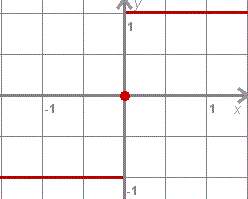
\includegraphics[scale=0.5]{resources/Signum_function.png}
              \end{center}
              }
        \item {
              整数部分函数(下取整函数) :$$
                  y = [x]
              $$

              在数学和计算机科学中,取整函数是一类将实数映射到相近的整数的函数.

              常用的取整函数有两个,分别是下取整函数和上取整函数.

              下取整函数即为取底符号,在数学中一般记作$[x]$或者$E(x)$,在计算机科学中一般记作$floor(x)$,表示不超过$x$的整数中最大的一个 : $$
                  [x] = \min\set{n \in \mathIntegerCollection | x \leq n}
              $$

              \functionTabular{$D = (-\infty,+\infty)$}{$R = [X] = \mathIntegerCollection$}{N/A}

              图像为 :

              \begin{center}
                  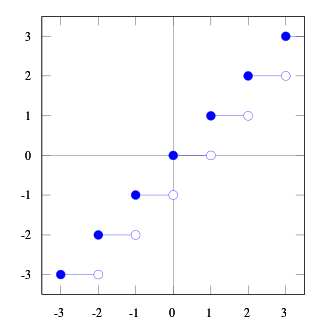
\includegraphics[scale=0.5]{resources/Floor_function.png}
              \end{center}

              下取整函数的符号用方括号$[x]$表示,称作高斯符号.
              }
        \item {
              小数部分函数(分数部分函数) : $$
                  y = (x) = x - [x]
              $$

              小数部分函数(decimal part function)亦称分数部分函数,是一种特殊的数论函数.$x$的小数部分记为${x}$,读作$x$的小数部分(或分数部分).小数部分函数被定义为${x}=x-[x]$,其中$[x]$是整数函数.$\{x\}$只能是0或正的纯小数,即$\{x\}$满足$0≤\{x\}<1$

              \functionTabular{$D = (-\infty,+\infty)$}{$R = \{X\} = (0,1)$}{N/A}

              图像为 :

              \begin{center}
                  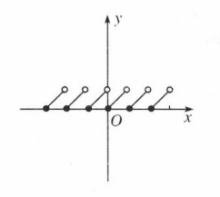
\includegraphics[]{resources/DecimalPartFunction.png}
              \end{center}
              }
        \item {
              狄利克雷函数 :

              问 : 是否周期函数都有最小周期?

              答 : 不是.

              反例 : 狄利克雷函数(Dirichlet function)$D(x)$ : $$
                  D(x)
                  =
                  \begin{cases}
                      0\qquad \mbox{$x$无理数} \\
                      1\qquad \mbox{$x$有理数}
                  \end{cases}
              $$

              \functionTabular{$D = (-\infty,+\infty)$}{$R = D(x) = (0,1)$}{偶函数}

              任何的有理数$r > 0$都是他的周期,没有最小周期.
              }
    \end{itemize}
}%一些特殊的函数结尾

}%函数结尾

}%映射与函数结尾

\section{数列极限}{

\subsection{实数系的连续性}{

\subsubsection{引入}{
    一切都得从实数系的诞生说起 :

    命题 : $\sqrt{2}$不是有理数.

    \begin{center}
        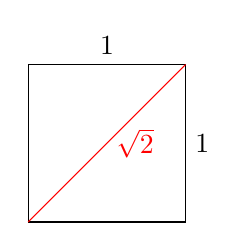
\begin{tikzpicture}
            \draw (0,0) -- (0,2) --node[above]{$1$} (2,2) -- node[right]{$1$} (2,0) -- cycle;
            \draw[red] (0,0) --node[right]{$\sqrt{2}$} (2,2);
        \end{tikzpicture}
    \end{center}

    使用反证法

    如果$\sqrt{2}$不是有理数,设其为有理数,即 : $$
        \sqrt{2} = \cfrac{n}{m}
    $$

    其中$n,m \in \mathNatureNumberCollection^+$且互质.

    那么$2 = \cfrac{n^2}{m^2}$,即$n^2 = 2m^2$

    则$n$是偶数.令$n = 2k$,则$m^2 = 2k^2$,因此$m$也是偶数,矛盾,得证.

    \qed

    换句话来说,在有理数上开根号不封闭,因此需要扩展数系.

    从几何上看是这样的 :

    \begin{center}
        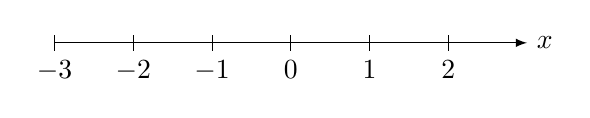
\begin{tikzpicture}% table%\begin{}[]%\addplot table[] {};%\end{}%\end{}
            \draw[-latex] (0,0) -- (6,0) node[right]{$x$};
            \foreach \i in {-3,...,2}{
                    \draw (\i + 3,-0.1) node[below]{$\i$} -- (\i + 3,0.1);
                }
        \end{tikzpicture}
    \end{center}

    \begin{itemize}
        \item {
              $\mathIntegerCollection$ :

              整数集上每一个数都对应其上的一个点,每两个点之间总有距离,点与点之间距离至少为1.称这一性质为\textcolor{red}{离散性}.

              因此可以说 : 整数集合具有集散性.
              }
        \item {
              $\mathRationalNumberCollection$ :

              有理数集合种每一个元素都可以在数轴上找到一个点与他对应,而且有理数很多,多到无法找到一个小区间,使得这个小区间内没有有理数.将这种性质称为\textcolor{red}{稠密性}.

              因此可以说 : 有理数集合具有稠密性.
              }
        \item {
              $\mathRealNumberCollection$

              长期以来人们一直只认识有理数,直到公元200年前的古希腊 :

              \begin{center}
                  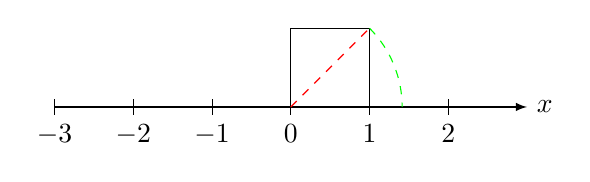
\begin{tikzpicture}
                      \draw[-latex] (0,0) -- (6,0) node[right]{$x$};
                      \foreach \i in {-3,...,2}{
                              \draw (\i + 3,-0.1) node[below]{$\i$} -- (\i + 3,0.1);
                          }
                      \draw (3,0) rectangle (4,1);
                      \draw[dashed,red] (3,0) -- (4,1);
                      \draw[dashed,green] (4,1) arc (45:0:{sqrt(2)});
                  \end{tikzpicture}
              \end{center}

              就这样,人们发现了一个在数轴上的点,对应的不是有理数.

              换句话说,尽管有理数集合在数轴上有稠密性,但是有空隙.

              于是又扩展了数系,将无限不循环小数(即无理数)加进了有理数系,就这样出现了实数集合$\mathRealNumberCollection$,自此运算又封闭了.

              因此实数是有理数集合和有理数集合的并,即 : $$
                  \mathRealNumberCollection = \set{x | x \in \mathRationalNumberCollection \lor x\mbox{是无理数}}
              $$

              引入的无理数填满了数轴上的空隙,现在数轴上每一个点都与实数集合中的一个元素对应,换句话来说: 实数集合布满了整个数轴,不留任何空隙.称这一性质为\textcolor{red}{连续性}.

              即 : 实数的连续性.

              实数集合有时候又被称为实数连续统.
              }
    \end{itemize}
}%引入结尾

\subsubsection{最大数与最小数}{
    首先提出以下概念 : 最大数与最小数.

    $S \subset \mathRealNumberCollection,\ S \neq \emptyset$,如果$S$是有限集,则$S$必有最大数和最小数.

    但是如果$S$是无限集,则$S$不一定有最大数与最小数.

    \begin{itemize}
        \item 如果$\exists \xi \in S$,使得$\forall x \in S$,有$x \leq \xi$,则称$\xi$是$S$中的最大数,记为$\xi = \max S$
        \item 如果$\exists \eta \in S$,使得$\forall x \in S$,有$x \geq \eta$,则称$\eta$是$S$中的最小数,记为$\eta = \min S$
        \item 显然,有限数集合一定有最大数和最小数.
        \item 但是无限数集合则不一定.
    \end{itemize}
}%最大数与最小数结尾

\subsubsection{上确界与下确界}{
    \begin{itemize}
        \item {
              上界 :

              \begin{itemize}
                  \item 设$S \subset \mathRealNumberCollection,\ S \neq \emptyset$,如果$\exists M \in \mathRealNumberCollection$,使得$\forall x \in S$,有$x \leq M$,则称$M$是$S$的一个上界,或称$S$有上界.
                  \item 设$U$是$S$上界的集合,则$U$没有最大数,但$U$必定有最小数.
                  \item $U$中的最小数记为$\beta = sup S$,称为$S$的上确界(supremum).
                  \item {
                        \(
                        \beta : \begin{cases}
                            \beta\mbox{是上界,即 : }\forall x \in S(x \leq \beta) \\
                            \beta\mbox{是最小上界,即 : }\forall \epsilon > 0 \exists x \in S (x > \beta - \epsilon)
                        \end{cases}
                        \)
                        }
              \end{itemize}
              }
        \item {
              下界 :

              \begin{itemize}
                  \item 设$S \subset \mathRealNumberCollection,\ S \neq \emptyset$,如果$\exists m \in \mathRealNumberCollection$,使得$\forall x \in S$,有$x \geq m$,则称$m$是$S$的一个下界,或称$S$有上界.
                  \item 设$L$是$S$下界的集合,则$L$没有最小数,但$L$必定有最大数.
                  \item $L$中的最大数记为$\alpha = inf S$,称为$S$的下确界(infimum).
                  \item {
                        \(
                        \alpha : \begin{cases}
                            \alpha\mbox{是下界,即 : }\forall x \in S(x \geq \alpha) \\
                            \alpha\mbox{是最大下界,即 : }\forall \epsilon > 0 \exists x \in S (x < \alpha + \epsilon)
                        \end{cases}
                        \)
                        }
              \end{itemize}
              }
    \end{itemize}
}%上确界与下确界结尾

\subsubsection{确界存在定理(实数系连续性定理)}{
\begin{itemize}
    \item 非空有上界的数集必有上确界.
    \item 非空有下界的子集必有下确界.
\end{itemize}

证明 : $$
    \forall_{x \in \mathRealNumberCollection} (x = [x] + (x))
$$

$$
    (x) = 0.a_1 a_2 \dots a_n \dots
$$
说明 :
\begin{itemize}
    \item 将$(x)$写成无限小数表示
    \item 如果是有限小数,那么后面加一列0.
    \item $0.a_1a_2 \dots a_p 000\dots\ (a_p \neq 0)$可以写成$0.a_1a_2 \dots (a_p-1)999\dots$,这两者等价$(1 = 0.99999\dots)$,但是一般使用前者的形式表示
\end{itemize}

设$S \subset \mathRealNumberCollection,S \neq \emptyset,$有上界,$S$可以表示成为 : $$
    S = \set{a_0 + a_1a_2 \dots a_n \dots | a_0 = [x],0.a_1a_2 \dots a_n \dots = (x),x \in S}
$$
\begin{enumerate}
    \item $S$有上界,取$S$中所有$a_0$的最大值,记为$\alpha_0$
    \item 作$S_0 = \set{x | x \in S \land [x] = \alpha_0}$,则$x \in S \land x \notin S \Rightarrow x < \alpha_0$
    \item 取$S_0$中$x$的小数表示中第1位小数的最大者为$\alpha_1$.
    \item 作$S_1 = \set{x | x \in S_1 \land x\mbox{的第一位小数为}\alpha_1}$,则$x \in S \land x \notin S_1 \Rightarrow x < \alpha_0 + 0.\alpha_1$
    \item 一般的,取$S_{n - 1}$中$x$的小数表示中第$n$位的最大者为$\alpha_n$
    \item 那么$S_n = \set{x | x \in S_{n - 1} \land x\mbox{的小数第$n$位为}\alpha_n}$,则$x \in S \land x \notin S_n \Rightarrow x < \alpha_0 + 0.\alpha_1\alpha_2 \dots \alpha_n \dots$
    \item \begin{enumerate}
              \item 得到了一串集合$S \supset S_0 \supset S_1 \supset S_2 \supset \dots \supset S_N \supset \dots$
              \item $\alpha_0 \in \mathIntegerCollection,\alpha_n(\alpha_1,\alpha_2,\dots,\alpha_n,\dots) \in \set{0,1,2,\dots,9}$
          \end{enumerate}
    \item 令$\beta = a_0 + 0.\alpha_1\alpha_2 \dots \alpha_n \dots$
    \item {
          \begin{proof}
              $\beta$是$S$的上确界 :

              \begin{enumerate}
                  \item $\beta$是$S$的上界 : \begin{enumerate}
                            \item $\forall x \in S$,或者$\exists n_0(x \notin S_{n_0})$,或者$\forall_{n \in \mathNatureNumberCollection}(x \in S_n)$
                            \item 若为前一种情况,则$x < \alpha_0 + 0.\alpha_1\alpha_2 \dots \alpha_n \leq \beta$
                            \item 若为后一种情况,则考虑$[x]$与$(x)$的每一位小数.发现$x = \beta$
                            \item 因此$\beta$是$S$的上界.
                        \end{enumerate}
                  \item $\beta$是最小上界,换句话来说 : $\forall \epsilon > 0,\beta - \epsilon$不是上界. : \begin{enumerate}
                            \item 可取$n_0 \in \mathIntegerCollection$,使$\cfrac{1}{10^{n_0}} < \epsilon$
                            \item 取$x \in S_{n_0}$,$[x] = \alpha_0$,前$n_0$位小数为$\alpha_1,\alpha_2,\alpha_{n_0}$
                            \item $\beta - x \leq \cfrac{1}{10^{n_0}} < \epsilon \Rightarrow x > \beta - \epsilon$
                            \item 因此$\beta$是$S$的上确界.下确界同理.
                        \end{enumerate}
              \end{enumerate}
          \end{proof}
          }
\end{enumerate}

此定理反映了实数系的连续性 :

假设数轴上存在一点为空隙,这一点既不是有理数也不是无理数,那么这个空隙左边的实数没有上确界,右边的实数没有下确界.

因此被称为实数系连续性存在定理.
}%确界存在定理结尾

\subsubsection{Dedekind切割定理}{
    \begin{itemize}
        \item 事实上实数连续性有多种等价的叙述方式,其中之一就是从有理数集的稠密性出发,使用Dedekind切割定理.
        \item 此定理是以有理数集$Q$的切割为基础导出无理数定义,进而定义整个实数系的.
    \end{itemize}

    \begin{itemize}
        \item {
              定义1 : 设两个非空有理数集合$A$和$B$满足以下条件 : $Q$ = $A \unionSet B$.且对任意的$a \in A$与$b \in B$,成立$a < b$,则称$A$和$B$构成$Q$的一个切割,记为$A/B$.

              从逻辑上讲,对有理数集合$Q$的任何切割$A/B$,下述情况有且仅有一种出现 : \begin{enumerate}
                  \item 集合$A$有最大数$a_0$,集合$B$没有最小数.
                  \item 集合$A$没有最大数,集合$B$有最小数$b_0$
                  \item 集合$A$没有最大数,集合$B$没有最小数.
                  \item 集合$A$有最大数,集合$B$有最小数.
              \end{enumerate}

              但情况$4$是不可能发生的.因为根据切割的定理,可知$a_0 < b_0$.而$\cfrac{a_0 + b_0}{2}$显然也是$Q$中的有理数,由$a_0 < \cfrac{a_0 +b_0}{2} < b_0$,即得到$\cfrac{a_0 + b_0}{2}$既不属于$A$也不属于$B$,这就与$Q = A \unionSet B$产生矛盾.

              对于情况$1$,称切割$A/B$确定了有理数$a_0$,对于情况$2$,称切割$A/B$确定了有理数$b_0$,而对情况$3$,由于$A/B$没有确定任何有理数,即$A$与$B$之间存在一个空隙,因此有必要引进一个新的数(即无理数)作为这一切割的确定对象,并且构成了实数集$\mathRealNumberCollection$.

              引入了后就可以保证对实数集的任意切割都不会出现空隙了.
              }
    \end{itemize}

    \paragraph{Dedekind切割定理的证明}{
        Dedekind切割定理 : 设$\hat{A} / \hat{B}$是$\mathRealNumberCollection$的一个切割,$\hat{A},\hat{B}$在这里意思是非空,则或者$\hat{A}$有最大数,或者$\hat{B}$有最小数.

        \begin{proof}
            设$A$是$\hat{A}$中所有有理数所构成的集合,$B$是$\hat{B}$中所有有理数构成的集合,则$A/B$是有理数集合$Q$的一个切割.由前面所述,对于切割$A/B$,下述三种情况有且仅有一种出现 :
            \begin{enumerate}
                \item 集合$A$有最大数$a_0$,集合$B$没有最小数.
                \item 集合$A$没有最大数,集合$B$有最小数$b_0$
                \item 集合$A$没有最大数,集合$B$没有最小数.
            \end{enumerate}

            对情况1,可以证明此时$a_0$是集合$\hat{a}$的最大数,而集合$\hat{B}$没有最小数 :

            用反证法.若有$\hat{a} \in \hat{A}$,成立$a_0 < \hat{a}$,则由有理数的稠密性,在区间$(a_0,\hat{a})$中必存在有理数$a_0$.由$a < \hat{a}$,可知$a \in A$,但$a > a_0$,与$a_0$就是$A$的最大数矛盾,说明$a_0$就是集合$\hat{A}$的最大数.

            对于任意的$\hat{b} \in \hat{B}$,因为$a_0 < \hat{b}$,于是在区间$(a_0,\hat{b})$中必存在有理数$b$.由$a_0 < b$,可知$b \in \hat{B}$,但是$b < \hat{b}$,这说明$\hat{B}$没有最小数.

            对于情况2,可类似证明此时$b_0$也是集合$\hat{b}$的最小数,而集合$\hat{A}$没有最大数.

            对于情况3,切割$A/B$确定一个无理数,将该无理数记为$c$,则对任意$a \in A$与任意$b \in B$,成立$a < c < b$.

            因为无理数$c \in \mathRealNumberCollection = \hat{A} \unionSet \hat{B}$,所以只有两种可能 : 或者$c \in \hat{A}$,或者$c \in \hat{B}$.若$c \in \hat{A}$,则$c$必是$\hat{A}$的最大数.若不是则存在$\hat{a} \in \hat{A}$,成立$c < \hat{A}$,在区间$(c,\hat{a})$中取有理数$a$,由$a < \hat{a}$,可知$a \in A$,但由$c < a$,又可知$a \in B$,这就产生矛盾.

            同理.若$c \in \hat{B}$,则$c$必是$\hat{B}$的最小数.

            综合情况$123$,可知Dedekind定理成立.

        \end{proof}
    }%Dedekind切割定理的证明结尾

}%Dedekind切割定理

}%实数系的连续性

\subsection{数列极限}{

    注:本章内容可用于级数.

    注:数列不是级数,级数需要求和数列不用.

    \subsubsection{数列}{
        若函数$f$的定义域为全体正整数集合$\mathNatureNumberCollection^n$,则称
        $$
            f : \mathNatureNumberCollection^+ \to \mathRealNumberCollection,\defFunction{n} \ (n \in \mathNatureNumberCollection^+)
        $$

        为数列.因正整数集$\mathNatureNumberCollection^+$的元素可按由小到大的顺序排列,所以数列$\defFunction{n}$也可以写作 :
        $$
            a_1,a_2,a_3,\dots,a_n,\dots,
        $$

        或者可以简记为${a_n}$,其中$a_n$称为该数列的通项.

        以下为一些例子 : \begin{itemize}
            \item $\set{\cfrac{1}{x}} : \cfrac{1}{1},\cfrac{1}{2},\cfrac{1}{3},\dots,\cfrac{1}{n},\dots$
            \item $\set{\cfrac{n}{n + 3}} : \cfrac{1}{4},\cfrac{2}{5},\cfrac{3}{6},\dots,\cfrac{n}{n + 3},\dots$
            \item $\set{n^2} : 1,4,9,\dots,n^2,\dots$
            \item $\set{(-1)^n} : -1,1,-1,1,\dots,(-1)^n,\dots$
        \end{itemize}

        简而言之,所谓数列就是按照正整数编号的一串数

        注意 : 与集合不同,数列允许重复,而且有顺序.
    }%数列结尾

    \subsubsection{邻域}{
        $a$点的$\epsilon$邻域$O(a,\epsilon) = (a - \epsilon, a + \epsilon)$,用集合的写法可表示为 : $$
            \set{x | x - \epsilon < x < x + \epsilon}
        $$
    }%邻域结尾

    \subsubsection{数列极限的定义}{
        设数列${x_n}$,存在$x_0$,若对于任意给定的$\epsilon > 0$,可以找到正整数$N$,使得当$n > N$时,有 : $$
            \absoluteValue{x_n - a} < \epsilon (\mbox{或者等价的说,} x \in O(a,\epsilon))
        $$

        则称数列${x_n}$收敛于$a,a$称为数列$x_n$的极限,记作
        $$
            \limNormal{n \to \infty}x_n = a
        $$

        若不存在$a$,即数列${x_n}$没有极限,则称${x_n}$不收敛,或者称${x_n}$发散.

        \begin{itemize}
            \item 此定义等价于 : 任给$\epsilon > 0$,若在$O(a,\epsilon)$之外数列${x_n}$中的项至多只有有限个,则称数列${x_n}$收敛域极限$a$.
            \item 由此定义可知,一个数列收敛的话,收敛于那个数,这与数列的前有限项无关,因此数列改动有限项不影响数列的收敛性和极限.
            \item {
                  $\cfrac{1}{n} : 1,\cfrac{1}{2},\dots$此数列以$0$为极限

                  以零为极限的变量(此处的变量是数列)通常称为\textcolor{red}{无穷小量}.

                  $$
                      \limNormal{n \to \infty}x_n = a \Rightarrow \set{x_n - a}\mbox{是无穷小量}
                  $$
                  }
        \end{itemize}
    }%数列极限的定义结尾

    \subsubsection{一些例题}{
        \begin{enumerate}
            \item {
                  用定义证明$\set{\cfrac{n}{n + 3}}$的极限为1.

                  \begin{proof}
                      对任意给定的$\epsilon > 0$ : $$
                          \absoluteValue{\cfrac{n}{n + 3} - 1} = \cfrac{3}{n + 3} < \epsilon \Leftrightarrow n > \cfrac{3}{\epsilon} - 3
                      $$

                      取$N = \mediumBigCase{\cfrac{3}{\epsilon}} + 1$,当$n > N$时,必定满足$$
                          \absoluteValue{\cfrac{n}{n + 3} - 1} < \epsilon
                      $$因此成立.

                  \end{proof}
                  }
            \item {
                  \begin{itemize}
                      \item $\set{n^2} : 1,4,9,16,\dots$
                      \item $\set{(-1)^n} : -1,1,-1,1,\dots$
                  \end{itemize}

                  根据定义,以上数列都是发散的.
                  }
            \item {
                  $0 < \absoluteValue{q} < 1$,证明$\set{q^n}$是无穷小量.

                  \begin{proof}
                      对任意的$\epsilon > 0$ : $$
                          \absoluteValue{q^n - 0} = \absoluteValue{q^n} < \epsilon
                      $$
                      $$
                          \Leftrightarrow n\lg\absoluteValue{q} < \lg\epsilon \Leftrightarrow n > \cfrac{\lg \epsilon}{\lg\absoluteValue{q}}
                      $$

                      于是$N$只要取任意大于这玩意的正整数即可,取$N = max\bigCase{\mediumBigCase{\cfrac{\lg \epsilon}{\lg \absoluteValue{q}}},1}$当$n > N$时,$\absoluteValue{q^n - 0} = \absoluteValue{q^n} < \epsilon$

                  \end{proof}

                  注 : 根据对数列极限的定义的讨论,$N$取的太大没啥意义,可以只考虑绝对值很小的$\epsilon > 0$,不妨考虑任意给定的$0 < \epsilon < \absoluteValue{q}$.则$N$可取为$\mediumBigCase{\cfrac{\lg \epsilon}{\lg \absoluteValue{q}}}$,即$\mediumBigCase{\log_{\absoluteValue{q}}\epsilon}$,当$n > N$时,成立$\absoluteValue{q^n - 0} < \epsilon$

                  根据数列极限的定义来证明某一数列收敛,其关键是对任意给定的$\epsilon > 0$寻找正整数$N$.在上面的立体中,$N$都是通过解不等式$\absoluteValue{x_n - a} < \epsilon$来得出的.但在大多数情况下,这个不等式并不容易解.实际上,数列极限的定义并不要求取到最好的$N$,所以在证明中常常对$\absoluteValue{x_n - a}$适度的做一些放大处理,这是种常用的技巧.以下是一些例子,描述了怎么使用这个技巧 :
                  }
            \item {
                  证明$\limNormal{n \to \infty}\sqrt[n]{a} = 1,\ (a > 1)$

                  \begin{proof}
                      对任意给定的$\epsilon > 0$,令$\absoluteValue{\sqrt[n]{a} - 1} < \epsilon$

                      令$\sqrt[n]{a} - 1 = y_n,\ y_n > 0$,则$\sqrt[n]{a} = 1 + y_n,\ a = (1 + y_n)^n$,使用二项式定理展开后很明显 : $$
                          a = 1 + ny_n + \mathCombination{n}{2}y^2_n +  \dots + y^n_n > 1 + ny_n \Rightarrow y_n < \cfrac{a - 1}{n}
                      $$
                      换而言之 : $$
                          \sqrt[n]{a} - 1 = y_n < \cfrac{a - 1}{n} < \epsilon
                      $$
                      那么$n$只要取到$n > \cfrac{a - 1}{\epsilon}$即可,取$\mediumBigCase{\cfrac{a - 1}{\epsilon}} + 1$

                      当$n > N$时,$\absoluteValue{\sqrt[n]{a} - 1} = y_n < \cfrac{a - 1}{n} < \epsilon$

                  \end{proof}
                  }
            \item {
                  证明$\limNormal{n \to \infty}\cfrac{n^2 + 1}{2n^2 - 7n} = \cfrac{1}{2}$

                  \begin{proof}
                      对任意给定的$\epsilon > 0$ : $$
                          \absoluteValue{\cfrac{n^2 + 1}{2n^2 - 7n} - \cfrac{1}{2}} = \absoluteValue{\cfrac{7n + 2}{2n(2n - 7)}}\stackrel{n > 3}{=}\cfrac{7n + 2}{2n(2n - 7)} < \cfrac{8n}{4n^2} \cdot 2 = \cfrac{4}{n}
                      $$
                      注 : 此时要求这个不等式成立的话$n$要满足$n > 6$

                      取$N = max\set{\mediumBigCase{\cfrac{4}{\epsilon}},6}$,当$n > N$,$\absoluteValue{\cfrac{n^2}{2n^2 - 7n} - \cfrac{1}{2}} = \absoluteValue{\cfrac{7n + 2}{2n(2n - 7)}} < \cfrac{4}{n} < \epsilon$

                  \end{proof}
                  }
            \item {
                  设$\limNormal{n \to \infty}a_n = a$,证明$\limNormal{n \to \infty}\cfrac{a_1 + a_2 + \dots + a_n}{n} = a$

                  \begin{proof}
                      分两步 :

                      \begin{enumerate}
                          \item {
                                设$a = 0$,对于任意给定的$\epsilon > 0$,存在$N_1$,当$n > N_1$时,$\absoluteValue{a_n} < \cfrac{\epsilon}{2}$

                                $$
                                    \cfrac{a_1 + a_2 + ... + a_n}{n} = \cfrac{a_1 + a_2 + ... + a_{N_1}}{n} + \cfrac{a_{N_1 + 1} + a_{N_1 + 2} + \dots + a_n}{n}
                                $$
                                此时后一项的绝对值必定小于$\cfrac{\epsilon}{2}$

                                回过头,此时第一项已经是个固定的数了,于是取$N > N_1$,使$n > N$时,$\absoluteValue{\cfrac{a_1 + a_2 + \dots + a_{N_1}}{n}} < \cfrac{\epsilon}{2}$

                                于是由三角不等式 : $$
                                    \absoluteValue{\cfrac{a_1 + a_2 + \dots + a_n}{n}} = \absoluteValue{\cfrac{a_1 + a_2 + ... + a_{N_1}}{n} + \cfrac{a_{N_1 + 1} + a_{N_1 + 2} + \dots + a_n}{n}}
                                $$
                                $$
                                    \leq \absoluteValue{\cfrac{a_1 + a_2 + ... + a_{N_1}}{n}} + \absoluteValue{\cfrac{a_{N_1 + 1} + a_{N_1 + 2} + \dots + a_n}{n}} < \cfrac{\epsilon}{2} + \cfrac{\epsilon}{2} = \epsilon
                                $$
                                }
                          \item {
                                $a \neq 0$,$\set{a_n - a}$是无穷小量.

                                $$
                                    \limNormal{n \to \infty}\bigCase{\cfrac{a_1 + a_2 + \dots + a_n}{n} - a} = \limNormal{n \to \infty}\cfrac{(a_1 - a) + (a_2 - a) + \dots + (a_n - a)}{n} = 0
                                $$
                                }
                      \end{enumerate}

                  \end{proof}
                  }
        \end{enumerate}
    }%一些例题结尾

    \subsubsection{数列极限的性质}{
        \begin{enumerate}
            \item {
                  极限的唯一性 : 若$\limNormal{n \to \infty}x_n = a,\limNormal{n \to \infty}x_n = b$,则$a = b$.

                  \begin{proof}
                      $\forall \epsilon > 0$ : \begin{itemize}
                          \item $\exists N_1,\forall n > N_1 : \absoluteValue{x_n - a} < \cfrac{\epsilon}{2}$
                          \item $\exists N_2,\forall n > N_2 : \absoluteValue{x_n - b} < \cfrac{\epsilon}{2}$
                      \end{itemize}
                      取$N = max\set{N_1,N_2},\forall n > N$,由三角不等式 : $$
                          \absoluteValue{a - b} = \absoluteValue{a - x_n + x_n - b} \leq \absoluteValue{x_n - a} + \absoluteValue{x_n - b} < \epsilon
                      $$
                      由$\epsilon$任意小可知,$a = b$.

                  \end{proof}
                  }
            \item {
                  数列的有界性(收敛数列必有界) :
                  \begin{itemize}
                      \item $\set{x_n}$,若$\exists M \in R,\forall n \in N^+$,成立$x_n \leq M$,则$M$是数列的一个上界,或称$\set{x_n}$有上界.
                      \item $\set{x_n}$,若$\exists M \in R,\forall n \in N^+$,成立$x_n \geq M$,则$M$是数列的一个下界,或称$\set{x_n}$有下界.
                  \end{itemize}

                  若$\set{x_n}$即有上界又有下界,则称$\set{x_n}$有界.

                  $\set{x_N}$有界的另一个定义 : $\exists X \in R,\forall n \in N^+$,成立$\absoluteValue{x_n} \leq X$

                  \begin{proof}
                      收敛数列必有界,设$\set{x_n}$收敛于$a$

                      由极限的定义,取$\epsilon = 1,\exists N,\forall n > N : a - 1 < x_n < a + 1$

                      取$M = max\set{x_1,x_2,\dots,x_N,a + 1},m = min\set{x_1,x_2,\dots,x_N,a - 1}$

                      显然对于$\absoluteValue{x_n}$所有的项 : $$
                          \forall n \in N^+,m \leq x_n \leq M
                      $$
                      因为n大于N以后,开始收敛,所以想找上界的值,就去找N之前的最大值,并且不排除邻域的边界.

                  \end{proof}
                  }
        \end{enumerate}
    }%数列极限的性质结尾

    \subsubsection{O'Stolz(stolz)定理}{
        设$(a_n)(n > 1)$和$(b_n)(n > 1)$为两个实数数列.若$b_n$为从某项开始严格单调的无界正数数列,且有穷极限
        $$
            \limNormal{n \to \infty}\cfrac{a_{n + 1} - a_n}{b_{n + 1} - b_n} = L
        $$

        存在,则 :
        $$
            \limNormal{n \to \infty}\cfrac{a_n}{b_n} = L
        $$

        其中$L$可以为有限实数或正/负无穷.

        该定理虽然主要被用于处理数列不定型极限,但该定理在没有$\limNormal{n \to \infty}a_n = \infty$这一条件时也是成立的.虽然该定理通常是以分母$b_n$为正数数列的情形加以叙述的,但注意到该定理对分子$a_n$的正负没有限制,所以原则上把对数列$b_n$的限制条件按替换为"严格单调递减且趋于负无穷大"也是没问题的.

        与洛必达的迭代用法类似,在尝试使用此定理考察数列极限时,如果发现两个数列差分的商任然是不定型,那么可以继续用.

        注意 : 与洛必达类似,判定条件不存在不能认定极限本身不存在.
    }%O'Stolz(stolz)定理结尾

}%数列极限结尾

}%数列极限结尾

}%数学分析结尾
  %*线性代数/高等代数
  % \section{线性代数}{

  \subsection{向量相关}{

      \subsubsection{标量}{
          标量(scalar),又称纯量,是只有大小,没有方向,可以用实数表示的一个量.实际上标量就是实数,叫他标量只是为了区别于向量.

          标量可以是负数.
      }%标量结尾

      \subsubsection{向量}{
          向量(euclidean vector,物理,工程等也称作矢量,欧几里得向量)是指一个同事具有大小和方向,而且满足平行四边形法则的几何对象.理论数学中向量的定义为任何在向量空间中的元素.一般的,同时具有大小和方向两个性质的几何对象即可认为是向量.向量常常在符号上加以箭头标识来区别于其他两.与向量相对的概念称为标量(数量),即只有大小,绝大多数情况下没有方向,不满足平行四边形法则的量.

          在线性代数中,向量场采用更为抽象的向量空间(也称为线性空间)来定义.向量是所谓向量空间中的基本构成元素.
      }%向量结尾

      \subsubsection{向量表示法}{
          注 : 本笔记默认向量记作头上带一个箭头的符号.比如向量$\alpha$就记作$\vec{\alpha}$

          \begin{itemize}
              \item {
                    向量的代数表示 :

                    代数表示指在指定了一个坐标系之后,用一个向量在该坐标系下的坐标表示该向量.兼具了符号的抽象性和几何形象性,因此具有最高的实用性,被广泛采用与需要定量分析的情形.对于自由向量,将向量的起点平移到坐标原点后,向量就可以用一个坐标系下的一个点来表示,该点的坐标值即向量的终点坐标.

                    设有一向量$\vec{\alpha}$,有坐标系$S$,在$S$中定义好若干个特殊的基本项链(称为基向量,各个基向量共同组成该坐标系下的基)$\vec{e_1},\vec{e_2},\dots,\vec{e_n}$置换,则向量在各个基向量下的投影值即为对应的分量值,各个分量值组成了该向量在坐标系$S$下可唯一表示的一个有序数组(即坐标),且与向量终点一一对应.

                    在矩阵运算中,向量更多的被写成类似于矩阵的列向量或者行向量.在线性代数中所指的向量默认为列向量.比如一个向量$\vec{\alpha} = (a,b,c)$,可写成 : $$
                        \vec{\alpha} = \begin{bmatrix}
                            \alpha_1 \\
                            \alpha_2 \\
                            \alpha_3 \\
                        \end{bmatrix}
                    $$
                    或者行向量的形式 : $$
                        \vec{\alpha} = \begin{bmatrix}
                            \alpha_1 & \alpha_2 & \alpha_3
                        \end{bmatrix}
                    $$

                    列向量和行向量都可以被视为矩阵.
                    }
              \item {
                    向量的几何表示 :

                    直观上,向量通常被标示为一个带箭头的有向线段.线段的长度表示向量的大小(或称模长),向量的方向即箭头所指的方向,可以记为$\vec{\alpha}$.该种表示的优点是具有强烈的几何直观形象性,缺点是在纸面上作图繁琐,不便定量分析 :

                    \begin{center}
                        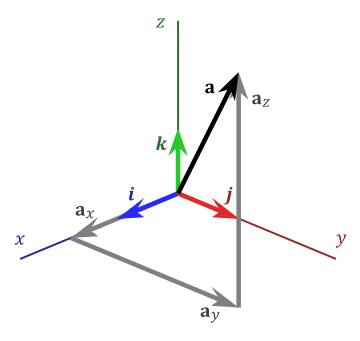
\includegraphics[scale=0.5]{resources/Vector_picture.png}
                    \end{center}
                    }
          \end{itemize}
      }%向量表示法

      \subsubsection{向量空间}{
          \begin{itemize}
              \item 向量空间是现代数学中的一个基本概念.是线性代数研究的基本对象.
              \item 向量空间的一个直观模型是向量几何,几何上的向量及相关的运算即向量加法,标量乘法,以及对运算的一些限制如封闭性,结合律,已大致地描述了"向量空间"这个数学概念的直观形象.
              \item 在现代数学中,"向量"的概念不仅限于此,满足下列公理的任何数学对象都可被当作向量处理.譬如,实系数多项式的集合在定义适当的运算后构成向量空间,在代数上处理是方便的.单变元实函数的集合在定义适当的运算后,也构成向量空间,研究此类函数向量空间的数学分支称为泛函分析.
          \end{itemize}

          给定域$F,F$上的向量空间$\vecSpace$是一个集合,其上定义了两种二元运算:

          \begin{itemize}
              \item 向量加法$+$ : $\vecSpace \times \vecSpace \to \vecSpace$,把$\vecSpace$中的两个元素$\vec{u}$和$\vec{v}$映射到$\vecSpace$中另一个元素,记为$\vec{u} + \vec{v}$
              \item 标量乘法$\cdot$ : $F \times \vecSpace \to \vecSpace$,把$F$中的一个元素$a$和$\vecSpace$中的一个元素$\vec{u}$变为$\vecSpace$中的另一个元素,记作$a \cdot \vec{u}$
          \end{itemize}

          V中的元素称为向量,相对地,F中的元素称为标量.

          而集合V满足以下公理才构成一个向量空间(对F中的任意元素a,b以及V中的任意元素u,v,w都成立):

          \begin{center}
              \begin{tabular}{|l|l|}
                  \hline
                  向量加法的结合律           & $\vec{u} + (\vec{v} + \vec{w}) = (\vec{u} + \vec{v}) + \vec{w}$                                            \\
                  \hline
                  向量加法的交换律           & $\vec{u} + \vec{v} = \vec{v} + \vec{u}$                                                                    \\
                  \hline
                  向量加法的单位元           & 存在一个零向量$\vec{0} \in \vecSpace$,使得对任意$\vec{u} \in \vecSpace$都满足$\vec{u} + \vec{0} = \vec{u}$ \\
                  \hline
                  向量加法的逆元素           & 对任意$\vec{v} \in \vecSpace$都存在其逆元素$-\vec{v}$,使得$\vec{v} + (-\vec{v}) = \vec{0}$                 \\
                  \hline
                  标量乘法与标量的域乘法相容 & $a(\vec{u} + \vec{v}) = a\vec{u} + a\vec{v}$                                                               \\
                  \hline
                  标量乘法的单位元           & 域$F$存在乘法单位元$1$满足$1\vec{v} = \vec{v}$                                                             \\
                  \hline
                  标量乘法对向量加法的分配律 & $a(\vec{u} + \vec{v}) = a\vec{u} + a\vec{v}$                                                               \\
                  \hline
                  标量乘法对域加法的分配律   & $(a + b)\vec{v} = a\vec{v} + b\vec{v}$                                                                     \\
                  \hline
              \end{tabular}

              向量空间的公理定义
          \end{center}

          由这些公理可以推出以下性质 :

          \begin{itemize}
              \item 零向量$\vec{0}$是唯一的.
              \item 对任意$a \in F,a \cdot \vec{0} = \vec{0}$.
              \item 对任意$\vec{u} \in \vecSpace,0 \times \vec{u} = \vec{0}$($0$是$F$的加法单位元).
              \item 如果$a \cdot \vec{u} = \vec{0}$,那么要么$a = 0$,要么$\vec{u} = \vec{0}$.
              \item 向量加法的逆向量$\vec{v}$是唯一的,记作$-\vec{v},\vec{u} + (-\vec{v})$也可以写称$\vec{u} - \vec{v}$,两者都是标准的.
              \item 对任意$\vec{u} \in \vecSpace,-1 \cdot \vec{u} = -\vec{u}$
              \item 对任意$a \in F$以及$\vec{u} \in \vecSpace,(-a) \cdot \vec{u} = -(a \cdot \vec{u}) = a \cdot (-\vec{u})$
          \end{itemize}
      }%向量空间结尾

  }%向量相关结尾

 }%线性代数结尾
  %*离散数学
  \chapter{离散数学}{

\section{前置知识}

\section{集合论}{

\subsection{集合论的主要内容}{
  \begin{itemize}
    \item 研究对象 : 集合,关系,函数,自然数,基数
    \item 研究思想 : 以逻辑为基础,以集合为工具,表示和构造各种数学对象
    \item 研究内容 : \begin{itemize}
            \item 集合的基本概念 : 集合之间的关系,运算,恒等式
            \item 二元关系 : 表示,性质,函数,等价关系,序关系
            \item 自然数 : 皮亚诺系统,自然数的运算,性质
            \item 基数 : 有序集于无穷集,基数的比较
            \item 良序,超限归纳法
          \end{itemize}
  \end{itemize}
}%集合论的主要内容结尾

\subsection{集合论中的问题}{
  \begin{itemize}
    \item 如何给集合下定义?
    \item 如何用集合去定义关系,函数,自然数?
    \item 如何比较集合的大小?
    \item 能否把每个集合的元素依次列举出来?
    \item 有没有最大的集合?
  \end{itemize}
}%集合论中的问题结尾

\subsection{集合的表示}{
  \begin{itemize}
    \item {
          列举法 :

          列出集合中的全体元素,元素之间用逗号分开,然后用花括号括起来,比如 : $A = \{a,b,c,d\},B = \{2,4,6,\dots\}$.
          }
    \item {
          描述法 :

          用谓词$P(x)$表示$x$具有性质$P$,用$\{x | P(x)\}$表示具有性质$P$的集合.例如 : $P_1(x)$表示$x$是英文字母,$P_2(x)$表示$x$是十进制数字,$C = \{x | P_1(x)\}$表示26个英文字母的集合,$D = \{x | P_2(x)\}$表示10个十进制数字的集合.
          }
  \end{itemize}
}%集合的表示结尾

\subsection{描述集合的注意事项}{
  \begin{enumerate}
    \item 集合中的元素是各不相同的.
    \item 集合中的元素不规定顺序.
    \item {
          集合的两种表示法可以互相转化,例如,$B={2,4,6,...}$可用描述法表示为$B=\{x|x>0\mbox{且x是偶数}\}$或$B=\{x|x=2(k+1),\mbox{k为非负整数}\}$.
          }
  \end{enumerate}
}%描述集合的注意事项结尾

\subsection{常用的集合}{
  \begin{itemize}
    \item $\mathNatureNumberCollection$: 自然数集合 $\mathNatureNumberCollection = {0,1,2,3,\dots}$
    \item $\mathIntegerCollection$: 整数集合 $\mathIntegerCollection = {0, \pm 1, \pm 2, \dots} = {\dots, -2, -1, 0, 1, 2, \dots}$
    \item $\mathRationalNumberCollection$: 有理数集合
    \item $\mathRealNumberCollection$: 实数集合
    \item $\mathComplexNumberCollection$: 复数集合
  \end{itemize}
}%常用的集合结尾

\subsection{集合之间的关系}{

\subsubsection{子集}{
  设$A,B$为二集合,若$B$中的元素都是$A$中的元素,则称$B$是$A$的子集,也称$A$包含$B$,或者$B$包含于$A$,记作$B \subseteq A$,其符号化形式为 : $$
    B \subseteq A \Leftrightarrow \forall x (x \in B \to x \in A)
  $$
  若$B$不是$A$的子集,则记作$B \subsetneq A$,其符号化形式为 : $$
    B \subsetneq A \Leftrightarrow \exists x (x \in B \land x \notin A)
  $$
}%子集结尾

\subsubsection{有限集和无限集}{
  \begin{itemize}
    \item 有限集,即元素数量优先的集合,定义叙述为 : $S$是由$n$个元素组成的集合($n$是非负正整数,包含0),则称$S$为有限集.
    \item 无限集:不是有限集的集合都是无限集.
  \end{itemize}
}%有限集和无限集结尾

\subsubsection{可列集}{
  可列集是无限集的一种,如果某无限集$S$中的元素可以按某种规则排成一列,并且无重复,无遗漏,则称该$S$为可列集.

  此时$S$可以被用列举法或者描述法表示.

  任何无限集都包含可列集,但是无限集本身不一定是可列集.

  另外,可列个可列集的并也是可列集.

}%可列集结尾

\subsubsection{相等}{
  设$A,B$为二集合,若$A$包含$B$且$B$包含$A$,则称$A$与$B$相等,记作$A = B$,符号化形式为 : $$
    A = B \Leftrightarrow \forall x (x \in B \leftrightarrow x \in A)
  $$
}%相等结尾

\subsubsection{集合之间包含关系的性质}{
  设$A,B,C$为三个集合,则以下三命题为真 :

  \begin{enumerate}
    \item $A \subseteq A$;
    \item 若$A \subseteq A$且$A \neq B$,则$B \subsetneq A$;
    \item 若$A \subseteq B$且$B \subseteq C$,则$A \subseteq C$
  \end{enumerate}
}%集合之间包含关系的性质结尾

\subsubsection{真子集}{
  设$A,B$为二集合,若$A$为$B$的子集且$A \neq B$,则称$A$为$B$的真子集,或者又称$B$真包含$A$,记作$A \subset B$,符号化形式为 : $$
    A \subset B \Leftrightarrow A \subseteq B \land A \neq B
  $$
  若$A$不是$B$的真子集,则记作$A \notRealSubset B$,其符号化形式为 : $$
    A \notRealSubset B \Leftrightarrow \exists x (x \in A \land x \notin B) \land A \neq B
  $$

  设$A,B,C$为三个集合,则以下命题为真 :

  \begin{enumerate}
    \item $A \notRealSubset A$;
    \item 若$A \subset B$,则$B \notRealSubset A$;
    \item 若$A \subset B$,且$B \subset C$,则$A \subset C$
  \end{enumerate}
}%真子集结尾

\subsubsection{空集}{
  不拥有任何元素的集合称为空集合,简称空集,记作$\emptyset$(读作ugh)

  比如$\{x | x^2 + 1 = 0 \land x \in \mathRealNumberCollection\}$和$\{(x,y) | x^2+y^2 < 0 \land x,y \in \mathRealNumberCollection\}$都是空集.

  注意 :

  \begin{itemize}
    \item 空集是一切集合的子集,
    \item 空集是唯一的
    \item 空集是最小的集合.
  \end{itemize}
}%空集结尾

\subsubsection{全集}{
  如果限定所讨论的集合都是某个集合的子集,则称该集合为全集,记作$\mathEverythingCollection$.

  从定义可以看出,全集是相对的,视具体情况而定,因此不唯一.

  比如 : 讨论区间$(a,b)$上的实数的性质时,可以取$(a,b)$为全集,也可以取$[a,b),(a,b],(a , +\infty),\mathRealNumberCollection$等为全集.

  给定若干个集合之后,都可以找到包含它们的全集.在今后讨论中,所涉及的集合都可以看成是某个全集$\mathEverythingCollection$的子集.
}%全集结尾

\subsubsection{集合的元素个数/集合的基数/集合的势}{
  $\emptyset$为$0$元集,含1个元素的集合为单元集或1元集,含两个元素的集合为2元集,依次类推,含$n$个元素的集合称为$n$元集$(n \geq 1)$.

  一个集合$A$所包含的元素数目称为该集合的基数或势(cardinality).记作$\absoluteValue{A}$或者$\#A$或$card(A)$

  当$A$中的元素个数为有限数时($\absoluteValue{A} < \infty$),$A$称为有穷集或有限集,否则称为无限集或者无穷集.
}%集合的元素个数结尾

\subsubsection{幂集}{
  设$A$为一个集合,称由$A$的全体子集组成的集合为$A$的幂集,记作$\powerSetOf{A}$.

  用描述法可以表示为 $\powerSetOf{A} = \{x | x \subseteq A\}$

  注意 :

  \begin{itemize}
    \item 在概率论中也会用$\powerSetOf{A}$来表示事件$A$的概率,两者虽然不相同但是定义是一样的.
    \item 为了避免混淆,也可以用$2^A$表示$A$的幂集.
    \item 这并不是没有道理,设集合$A$的元素个数$\absoluteValue{A} = n$,则$\absoluteValue{\powerSetOf{A}} = 2^n$
  \end{itemize}
}%幂集结尾s

\subsubsection{求幂集的步骤}{
  为了求出给定集合$A$的幂集,先求$A$的由低到高的所有子集,再将它们组成集合.

  设$A = \{a,b,c\}$,求$\powerSetOf{A}$的步骤如下 :

  0元子集为$\emptyset$;1元子集为$\{a\},\{b\},\{c\}$;2元子集为$\{a,b\},\{a,c\},\{b,c\}$;3元子集为$\{a,b,c\} = A$;

  所以,$A$的幂集为 : $$
    \powerSetOf{A} = \{\emptyset,\{a\},\{b\},\{c\},\{a,b\},\{a,c\},\{b,c\},\{a,b,c\}\}
  $$
}%求全集的步骤结尾

\subsubsection{集族}{
除了幂集$\powerSetOf{A}$以外,还有其他形式的由集合构成的集合,统称为集族.若集族中的集合都赋予记号,则可得带指标集的集族.

设$\mathcal{A}$为一个集族,$S$为一个集合,若对于任意的$\alpha \in S$,存在唯一的$A_\alpha \in \mathcal{A}$与之对应,而且$\mathcal{A}$中的任意集合都对应$S$中的某一元素,则称$\mathcal{A}$是以$S$为指标集的集族,$S$称为$\mathcal{A}$的指标集.记为$\mathcal{A} = \{A_\alpha | \alpha \in S\}$,或$\mathcal{A} = \{A_\alpha\}_{\alpha \in S}$

如果把$\emptyset$看作集族,则称$\emptyset$为空集族.
}%集族结尾

\subsubsection{多重集}{
  设全集为$\mathEverythingCollection$,$\mathEverythingCollection$中元素可以不止一次在$A$中出现的集合$A$称为多重集.若$\mathEverythingCollection$中元素$a$在$A$中出现$k$次($k \geq 0$),则称$a$在$A$中重复度为$k$.

  例如 : 设全集$E = \{a,b,c,d,e\},A = \{a,a,b,b,c\}$为多重集,其中$a,b$的重复度为2,$c$的重复度为1,而$d,e$的重复度为0.

  集合可以看作重复度均$\leq 1$的多重集.
}%多重集结尾

}%集合之间的关系结尾

\subsection{集合的运算}{

  \subsubsection{并集}{
    设$A,B$为二集合,称由$A$和$B$的所有元素组成的集合为$A$与$B$的并集,记作$A \unionSet B$,称$\unionSet$为并元算符.

    $A \unionSet B$得到的集合,用描述法可以表示为 : $$
      A \unionSet B = \{x | x \in A \lor x \in B\}
    $$
    集合的并运算可以推广到有限个或可数个集合(初级并).

    设$A_1,A_2,\dots,A_n$为$n$个集合,$A_1,A_2,\dots,A_n,\dots$为可数个集合,则 : $$
      A_1 \unionSet A_2 \unionSet \dots \unionSet A_n = \{x | \exists i (1 \leq i \leq n \land x \in A_i)\}
    $$

    并集也可以写作类似求和的形式 : $$
      \updownUnion{n}{i = 1}A_i = A_1 \unionSet A_2 \unionSet \dots \unionSet A_n
    $$

  }%并集结尾

  \subsubsection{交集}{
    设$A,B$为二集合,称由$A$和$B$的公共元素组成的集合为$A$与$B$的交集,记作$A \intersectionSet B$,称$\intersectionSet$为并元算符.

    $A \intersectionSet B$的描述法表示为$$
      A \intersectionSet B = \{x | x \in A \land x \in B\}
    $$
    集合的交运算可以推广到有限个或可数个集合(初级交).

    设$A_1,A_2,\dots,A_n,\dots$为可数个集合,则 : $$
      A_1 \intersectionSet A_2 \intersectionSet \dots \intersectionSet A_n = \{x | \forall i (1 \leq i \leq n \to x \in A_i)\}
    $$

    同样的,也有这种简化形式 : $$
      \bigcap\limits_{i = 1}^{n}A_i = A_1 \intersectionSet A_2 \intersectionSet \dots \intersectionSet A_n
    $$
  }%交集结尾

  \subsubsection{不相交}{
    设$A,B$为二集合,若$A \intersectionSet B = \emptyset$,则称$A$和$B$是不交的.设$A_1,A_2,\dots$是可数个集合秒如果对于任意的$i \neq j$,都有$A_i \intersectionSet A_j = \neq$,则称$A_1,A_2,\dots$是互不相交的.

    设$A_n = \{x \in R | n - 1 < x < n\},n = 1,2,\dots$,则$A_1,A_2,\dots$是互不相交的.
  }%不相交结尾

  \subsubsection{相对补集}{
    设$A,B$为二集合,称属于$A$而不属于$B$的全体元素组成的集合为$B$对$A$的相对补集,记作$A - B$或$\complement_A B$.$A - B$的描述法表示为 : $$
      A - B = \{x | x \in A \land x \notin B\}
    $$
  }%相对补集

  \subsubsection{对称差}{
    设$A,B$为二集合,称属于$A$而不属于$B$,或属于$B$而不属于$A$的全体元素组成的集合为$A$与$B$的对称差,记作$A \oplus B$.

    $A \oplus B$的描述法表示为 : $$
      A \oplus B = \{x | (x \in A \land x \notin B) \lor (x \notin A \land x \in B)\}
    $$
    容易看出 : $$
      A \oplus B = (A - B) \unionSet (B - A) = (A \unionSet B) - (A \intersectionSet B)
    $$
  }%对称差结尾

  \subsubsection{绝对补集}{
    设$\mathEverythingCollection$为全集,$A \subseteq \mathEverythingCollection$, 称$A$对$\mathEverythingCollection$的相对补集为$A$的绝对补集,记作$A\absoluteCompletementSet$或${~}^\sim A$或$\complement_{\mathEverythingCollection} A$.

    $A\absoluteCompletementSet$的描述法表示为 : $$
      A\absoluteCompletementSet = \{x | x \in \mathEverythingCollection \land x \notin A\}
    $$
    因为$\mathEverythingCollection$是全集,所以$x \in \mathEverythingCollection$是真命题,于是 : $$
      A\absoluteCompletementSet = \{x | x \notin A\}
    $$
  }%绝对补集结尾

  \subsubsection{广义并集}{
    设$\mathcal{A}$为一个集族,称由$\mathcal{A}$中全体元素的元素组成的集合为$\mathcal{A}$的广义并,记作$\bigcup \mathcal{A}$("大并$\mathcal{A}$").

    $\bigcup \mathcal{A}$的描述法表示为 : $$
      \bigcup\mathcal{A} = \{x | \exists z (x \in z \land z \in \mathcal{A})\}
    $$

    设$\mathcal{A} = \{\{a,b\},\{c,d\},\{d,e,f\}\}$,则$\bigcup \mathcal{A} = \{a,b,c,d,e,f\}$.

    当$\mathcal{A}$是以$S$为指标集的集族时 : $$
      \bigcup\mathcal{A} = \bigcup\{A_\alpha | \alpha \in S\} = \bigcup_{\alpha \in S}A_\alpha
    $$
  }%广义并集结尾

  \subsubsection{广义交}{
    设$\mathcal{A}$为一个集族,称由$\mathcal{A}$中全体元素的元素组成的集合为$\mathcal{A}$的广义并,记作$\bigcap \mathcal{A}$("大并$\mathcal{A}$").

    $\bigcap \mathcal{A}$的描述法表示为 : $$
      \bigcap\mathcal{A} = \{x | \exists z (x \in z \land z \in \mathcal{A})\}
    $$

    设$\mathcal{A} = \{\{1,2,3\},\{1,a,b\},\{1,6,7\}\}$,则$\bigcap \mathcal{A} = \{1\}$.

    当$\mathcal{A}$是以$S$为指标集的集族时 : $$
      \bigcap\mathcal{A} = \bigcap\{A_\alpha | \alpha \in S\} = \bigcap_{\alpha \in S}\mathcal{A}_\alpha
    $$

    注意 : 当$A = \emptyset$时,$\intersectionSet \emptyset$无意义.
  }%广义交结尾

  \subsubsection{集合运算的优先级}{
    有以下几类 :

    \begin{itemize}
      \item 第一类运算(此类运算按照从左向右的顺序进行) : 绝对补,幂集,广义交,广义并等.
      \item 第二类运算(此类运算按照括号决定的顺序运算,多个括号并排或没有括号的部分按照从左向右的顺序运算) : 初级并,初级交,相对补,对称差等.
    \end{itemize}
  }%集合运算的优先级结尾

  \subsubsection{文氏图}{
    文氏图就是将集合与集合之间的关系以及一些运算的结果用图像进行表示.在文氏图中,用矩形代表全集,用元或者其他闭曲线的内部代表$\mathEverythingCollection$的子集,并将运算结果得到的集合用阴影部分表示.

    \begin{center}
      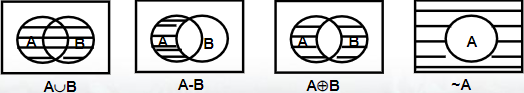
\includegraphics{resources/Venn's_diagram.png}
    \end{center}
  }%文氏图结尾

  \subsubsection{容斥原理(排斥原理)}{
    设$A_1,A_2,\dots,A_n$为$n$个集合,则 : $$
      \absoluteValue{\updownUnion{n}{i = 1}A_i} = \upDownSum{n}{i = 1}\absoluteValue{A_i} - \upDownSum{\ }{i < j}\absoluteValue{A_i \intersectionSet A_j} + \upDownSum{\ }{i < j < k}\absoluteValue{A_i \unionSet A_j \unionSet A_k} - \dots + (-1)^{n - 1}\absoluteValue{A_1 \unionSet A_2 \unionSet \dots \unionSet A_n}
    $$
  }%容斥原理结尾

}%集合之间的运算结尾

\subsection{基本集合恒等式}{
  设$\mathEverythingCollection$,$A,B,C$为$\mathEverythingCollection$的任意子集:

  \begin{enumerate}
    \item 幂等律 : $A \intersectionSet A = A, A \unionSet A = A$
    \item 交换律 : $A \unionSet B = B \unionSet A,A \intersectionSet B = B \intersectionSet A$
    \item 结合律 : $(A \unionSet B) \unionSet C = A \unionSet (B \unionSet C),(A \intersectionSet B) \intersectionSet C = A \intersectionSet (B \intersectionSet C)$
    \item 分配律 : $A \unionSet (B \intersectionSet C) = (A \intersectionSet B) \intersectionSet (A \unionSet C), A \intersectionSet (B \unionSet C) = (A \intersectionSet B) \unionSet (A \intersectionSet C)$
    \item 德$\cdot$摩根律 : \begin{itemize}
            \item 绝对形式 : $(A \unionSet B)\absoluteCompletementSet = A\absoluteCompletementSet \intersectionSet B\absoluteCompletementSet,(A \intersectionSet B)\absoluteCompletementSet = A\absoluteCompletementSet \unionSet B\absoluteCompletementSet$
            \item 相对形式 : $\mathEverythingCollection - (A \unionSet B) = (\mathEverythingCollection - A) \intersectionSet (\mathEverythingCollection - B),\mathEverythingCollection - (A \intersectionSet B) = (\mathEverythingCollection - A) \unionSet (\mathEverythingCollection - B)$
          \end{itemize}
    \item 吸收律 : $A \unionSet (A \intersectionSet B) = A,A \intersectionSet (A \unionSet B) = A$
    \item 零律 : $A \unionSet \mathEverythingCollection = E,A \intersectionSet \emptyset = \emptyset$
    \item 同一律 : $A \unionSet \emptyset = A,A \intersectionSet E = A$
    \item 排中律 : $A \unionSet A\absoluteCompletementSet = \mathEverythingCollection$
    \item 矛盾律 : $A \intersectionSet A\absoluteCompletementSet = \emptyset$
    \item 余补律 : $\emptyset\absoluteCompletementSet = \mathEverythingCollection,\mathEverythingCollection\absoluteCompletementSet = \emptyset$
    \item 双重否定律 : $(A\absoluteCompletementSet)\absoluteCompletementSet = A$
    \item 补交转换律 : $A - B = A \intersectionSet B\absoluteCompletementSet$
  \end{enumerate}
}%基本集合恒等式结尾

\subsection{集合恒等式推广到集族的情况}{
设$\{A_\alpha\}_{\alpha \in S}$为集族,$B$为一集合 :

\begin{itemize}
  \item 分配律 : $B \unionSet (\updownIntersection{~}{~}\{A_\alpha\}_{\alpha \in S}) = \updownIntersection{~}{\alpha \in S}(B \unionSet A_\alpha),B \intersectionSet (\updownUnion{~}{~}\{A_\alpha\}_{\alpha \in S}) = \updownUnion{~}{\alpha \in S}(B \intersectionSet A_\alpha)$
  \item 德$\cdot$摩根律 : \begin{itemize}
          \item 绝对形式: \begin{itemize}
                  \item $(\updownUnion{~}{~}\{A_\alpha\}_{\alpha \in S})\absoluteCompletementSet = \updownIntersection{~}{\alpha \in S}(A_\alpha\absoluteCompletementSet)$
                  \item$(\updownIntersection{~}{~}\{A_\alpha\}_{\alpha \in S})\absoluteCompletementSet = \updownUnion{~}{\alpha \in S}(A_\alpha\absoluteCompletementSet)$
                \end{itemize}
          \item 相对形式 : \begin{itemize}
                  \item $B - (\updownUnion{~}{~}\{A_\alpha\}_{\alpha \in S}) = \updownIntersection{~}{\alpha \in S}(B - A_\alpha)$
                  \item $B - (\updownIntersection{~}{~}\{A_\alpha\}_{\alpha \in S}) = \updownUnion{~}{\alpha \in S}(B - A_\alpha)$
                \end{itemize}
        \end{itemize}
\end{itemize}
}%集合恒等式推广到集族的情况结尾

\subsection{集合幂集运算的性质}{
  \begin{enumerate}
    \item $A \subseteq B$当且仅当$\powerSetOf{A} \subseteq \powerSetOf{B}$
    \item $\powerSetOf{A - B} \subseteq (\powerSetOf{A} - \powerSetOf{B}) \unionSet \{\emptyset\}$
  \end{enumerate}
}%集合幂集运算的性质结尾

\subsection{有序对与卡氏积}{

  \subsubsection{有序对(有序二元组)}{
    有序对又称有序二元组 : $$
      <a,b> = \{\{a\},\{a,b\}\}
    $$

    其中$a$是第一元素,$b$是第二元素.

    $<a,b>$也记作$(a,b)$.

    由于集合没有顺序,因此${a,b}$和${b,a}$是一样的.又称无序对,在公理集合论中有一条定义无序对的公理,称为无序对公理 : $$
      \mbox{如果$a,b$是集合,则\{a,b\}依然是集合}
    $$

    而在$<a,b>$中,$a$在每一个子集合中,而$b$只出现在其中一个子集合中,因此他们的地位不相等,所以在有序对中$a$是第一元素,$n$是第二元素.

    实际上是定义了一个数组,用这种方法来保证元素的顺序.

    接下来一章严格证明有序对的性质.
  }%有序对结尾

  \subsubsection{有序对性质的证明}{
    \begin{itemize}
      \item {
            引理1 : $\{x,a\} = \{x,b\} \Leftrightarrow a = b$

            叙述为 : 当集合$\{x,a\}$等于$\{x,b\}$当且仅当$a = b$.

            证明 : \begin{itemize}
              \item 充分性($\Leftarrow$) 是显然的,因此不证.
              \item 必要性($\Rightarrow$) 分两种情况 : \begin{enumerate}
                      \item $x = a.\ \{x,a\} = \{x,b\} \Rightarrow \{a,a\} = \{a,b\} \Rightarrow \{a\} = \{a,b\} \Rightarrow a = b$
                      \item $x \neq a.\ a \in \{x,a\} = \{x,b\} \Rightarrow a = b$.
                    \end{enumerate}
            \end{itemize}

            \qed
            }
      \item {
            引理2 : 若$\mathcal{A} = \mathcal{B} \neq \emptyset$.则 : \begin{enumerate}
              \item $\updownUnion{~}{~}\mathcal{A} = \updownUnion{~}{~}\mathcal{B}$
              \item $\updownIntersection{~}{~}\mathcal{A} = \updownIntersection{~}{~}\mathcal{B}$
            \end{enumerate}

            证明 : \begin{enumerate}
              \item $\forall x,x \in \updownUnion{~}{~}\mathcal{A} \Leftrightarrow \exists z(z \in \mathcal{A} \land x \in z) \Leftrightarrow \exists z(z \in \mathcal{B} \land x \in z) \Leftrightarrow x \in \updownUnion{~}{~}\mathcal{B}$
              \item $\forall x,x \in \updownIntersection{~}{~}\mathcal{A} \Leftrightarrow \forall z(z \in \mathcal{A} \land x \in z) \Leftrightarrow \forall z(z \in \mathcal{B} \land x \in z) \Leftrightarrow x \in \updownIntersection{~}{~}\mathcal{B}$
            \end{enumerate}

            \qed
            }
      \item {
            定理(性质1)--两个有序对相对,当且仅当他们的第一个元素和第二个元素分别相等 : $<a,b> = <c,d> \Leftrightarrow a = c \land b = d$

            证明 : \begin{itemize}
              \item ($\Leftarrow$) 显然,不证.
              \item{
                    ($\Rightarrow$) :

                    由引理2,$\set{\set{a},\set{a,b}} = \set{\set{c},\set{c,d}} \Rightarrow \updownIntersection{~}{~}\set{\set{a},\set{a,b}} = \updownIntersection{~}{~}\set{\set{c},\set{c,d}} \Rightarrow \set{a} = \set{c} \Leftrightarrow a = c$

                    又因为$<a,b> = <c,d> \Leftrightarrow \set{\set{a},\set{a,b}} = \set{\set{c},\set{c,d}} \Rightarrow \updownUnion{~}{~}\set{\set{a},\set{a,b}} = \updownUnion{~}{~}\set{\set{c},\set{c,d}} \Rightarrow \set{a,b} = \set{c,d}$

                    再由引理1,得出$b = d$.

                    \qed
                    }
            \end{itemize}
            }
      \item {
            推论 : $a \neq b \Rightarrow <a,b> \neq <b,a>$

            证明(反证) : $$
              <a,b> = <b,a> \Leftrightarrow a = b
            $$
            与$a \neq b$矛盾.

            \qed
            }
    \end{itemize}
  }%有序对性质的证明结尾

  \subsubsection{有序n元组}{
    \begin{itemize}
      \item {
            有序三元组 : $$
              <a,b,c> = <<a,b>,c>
            $$
            }
      \item {
            有序n($n > 2$)元组 : $$
              <a_1,a_2,\dots,a_n> = <<a_1,a_2,\dots,a_{n - 1}>,a_n>
            $$
            }
    \end{itemize}

    有以下定理 : $$
      <a_1,a_2,\dots,a_n> = <b_1,b_2,\dots,b_n> \Leftrightarrow a_i = b_i,i = 1,2,\dots,n
    $$
  }%有序n元组结尾

  \subsubsection{笛卡尔乘积集合(卡氏积)}{
    设$A,B$为两个集合,取$x \in A,y \in B$,构造有序对集合$\{(x,y)| x \in A \land y \in B\}$(属于$A$的$x$在前面,属于$B$的$y$在后面),将这样的集合记为笛卡尔乘积集合(又称为卡氏积) : $$
      A \times B = \set{<x,y>|x \in A \land y \in B}
    $$

    这种集合可以用来表示两个集合中元素的排列组合.

    举例,设$A = \set{\emptyset,a},B = \set{1,2,3}$,则 :

    \begin{itemize}
      \item $A \times B = \set{<\emptyset,1>,<\emptyset,2>,<\emptyset,3>,<a,1>,<a,2>,<a,3>}$
      \item $B \times A = \set{<1,\emptyset>,<1,a>,<2,\emptyset>,<2,a>,<3,\emptyset>,<3,a>}$
      \item $A \times A = \set{<\emptyset,\emptyset>,<\emptyset,a>,<a,\emptyset>,<a,a>}$
      \item \dots
    \end{itemize}
  }%笛卡尔乘积集合结尾

  \subsubsection{卡氏积的性质}{
    \begin{itemize}
      \item {
            卡氏积非交换性 : $A \times B \neq B \times A$(除非$A = B \lor A = \emptyset \lor B = \emptyset$)

            反证法反例 : 设$A = \set{1},B = \set{2}$ : $$
              A \times B = \set{<1,2>} \neq \set{<2,1>} = B \times A
            $$

            \qed
            }
      \item {
            卡氏积非结合性 : $(A \times B) \times C \neq A \times (B \times C)$(除非$A = \emptyset \lor B = \emptyset \lor C = \emptyset$)

            反证法反例 : $A = B = C = \set{1}$ : $$
              (A \times B) \times C = \set{<<1,1>,1>} \neq \set{<1,<1,1>>} = A \times (B \times C)
            $$

            \qed
            }
      \item {
            卡氏积分配律 :

            \begin{enumerate}
              \item $A \times (B \unionSet C) = (A \times B) \unionSet (A \times C)$
              \item $A \times (B \intersectionSet C) = (A \times B) \intersectionSet (A \times C)$
              \item $(B \unionSet C) \times A = (B \times A) \unionSet (C \unionSet A)$
              \item $(B \intersectionSet C) \times A = (B \times A) \intersectionSet (C \times A)$
            \end{enumerate}

            其中选一个证明 : $A \times (B \unionSet C) = (A \times B) \unionSet (A \times C)$.

            证明 : \begin{math}
              \forall <x,y>,<x,y> \in A \times (B \unionSet C) \\
              \Leftrightarrow x \in A \land y \in (B \unionSet C) \Leftrightarrow x \in A \land (y \in B \lor y \in C) \\
              \Leftrightarrow (x \in A \lor y \in B) \lor (x \in A \land y \in C) \\
              \Leftrightarrow (<x,y> \in A \times B) \lor (<x,y> \in A \times C) \\
              \Leftrightarrow <x,y> \in (A \times B) \unionSet (A \times C)
            \end{math}

            \qed
            }
    \end{itemize}
  }%卡氏积的性质结尾

  \subsubsection{卡氏积的图示}{
    放张图就一目了然了 :

    \begin{center}
      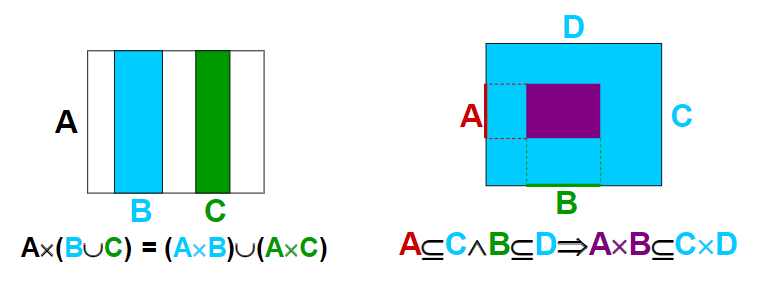
\includegraphics{resources/Set_DicarelProduct.png}
    \end{center}

    特别的 : $A = B = \mathRealNumberCollection$,则$A \times B = \mathRealNumberCollection \times \mathRealNumberCollection = \mathRealNumberCollection^2$,也就是笛卡尔平面直角坐标系.

    同样的,也有$R^3,R^n$


    $$
      A = \{x | x \in \mathRealNumberCollection \land a \leq x \leq b\}
    $$
    $$
      B = \{y | y \in \mathRealNumberCollection \land c \leq y \leq d\}
    $$
    $$
      C = \{z | z \in \mathRealNumberCollection \land e \leq z \leq f\}
    $$
    那么$A \times B$的图像表示就是 :
    \begin{center}
      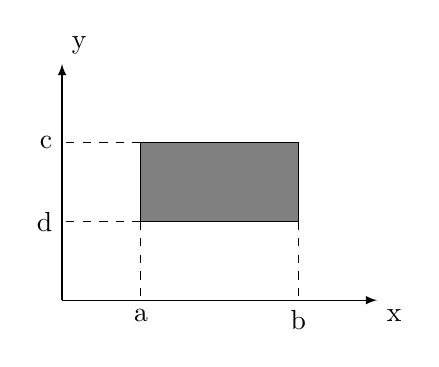
\begin{tikzpicture}
        \draw[-latex] (0,0) -- (4,0) node[below right]{x};
        \draw[-latex] (0,0) -- (0,3) node[above right]{y};
        \draw[fill = gray] (1,1) rectangle (3,2);
        \draw[dashed] (1,1) -- (1,0) node[below]{a};
        \draw[dashed] (3,1) -- (3,0) node[below]{b};
        \draw[dashed] (1,2) -- (0,2) node[left]{c};
        \draw[dashed] (1,1) -- (0,1) node[left]{d};
      \end{tikzpicture}
    \end{center}

    同样的,$A \times B \times C$表示的是空间中的一个立方体,这里就不画了(邪恶的tikz).
  }%卡氏积的图示结尾

  \subsubsection{n维卡氏积}{
    \begin{itemize}
      \item n维卡氏积 : $$
              A_1 \times A_2 \times \dots \times A_n = \set{<x_1,x_2,\dots,x_n> | x_1 \in A_1 \land x_2 \in A_2 \land \dots \land x_n \in A_n}
            $$
      \item $A^n = A \times A \times \dots \times A$
      \item $\absoluteValue{A_i} = n_i,i = 1,2,\dots,n \Rightarrow \absoluteValue{A_1 \times A_2 \times \dots \times A_n} = n_1 \times n_2 \times \dots \times n_n$.
      \item n维卡氏积性质于2维卡氏积类似.
    \end{itemize}
  }%n维卡氏积结尾

  \subsubsection{n维卡氏积的性质}{
    \begin{itemize}
      \item 非交换 : $A \times B \times C \neq B \times C \times A$\ (要求$A,B,C$均非空,且互不相等)
      \item 非结合 : (非二元运算)
      \item 分配律 : 例如 : $A \times B \times (C \unionSet D) = (A \times B \times C) \unionSet (A \times B \times D)$
      \item 其他 : 比如$A \times B \times C = \emptyset \Leftrightarrow A = \emptyset \lor B = \emptyset \lor C = \emptyset$.
    \end{itemize}
  }%n维卡氏积的性质结尾

}%有序对与卡氏积结尾

\subsection{二元关系}{

  \subsubsection{n元关系}{
    \begin{itemize}
      \item n元关系 : 其元素全是有序n元组的集合.
      \item 例1 : $F_1 = \set{<a,b,c,d>,<1,2,3,4>,<\alpha,\beta,\gamma,\delta>}$---$F_1$是3元关系.
      \item 例2 : $F_2 = \set{<a,b,c>,<\alpha,\beta,\gamma>,<A,B,C>}$---$F_2$是3元关系
    \end{itemize}
  }%n元关系结尾

  \subsubsection{二元关系}{
    \begin{itemize}
      \item 2元关系(关系) : 元素全是有序对的集合.
      \item 比如$A = \set{<A,B>,<1,2,3>,a,\alpha,1}$---如果$a,\alpha,1$不是有序对,那么$A$不是关系.
    \end{itemize}
  }%二元关系结尾

  \subsubsection{二元关系的记号}{
    \begin{itemize}
      \item{
            设$F$是二元关系,那么有三种记法 :

            \begin{itemize}
              \item 中缀(infix)记号 : $xFy$
              \item 前缀(prefix)记号 : $F(x,t),Fxy$
              \item 后缀(suffix)记号 : $\dependent{,xy} \in F,xyF$
            \end{itemize}
            }
      \item 例如 : $2 < 15 \Leftrightarrow <(2,15) \Leftrightarrow \dependent{2,15} \in <$
    \end{itemize}
  }%二元关系的记号结尾

  \subsubsection{A到B的二元关系}{
    \begin{itemize}
      \item {
            A到B的二元关系 : 是$A \times B$的任意子集.

            $R$是$A$到$B$的二元关系$\Leftrightarrow R \subseteq A \times B \Leftrightarrow R \in \powerSetOf{A \times B}$
            }
      \item 如果$\absoluteValue{A} = m,\absoluteValue{B} = n$,则$\absoluteValue{A \times B} = mn$,所以$\absoluteValue{P(A \times B)} = 2^{mn}$,也就是说$A$到$B$不同的二元关系共有$2^{mn}$个.
    \end{itemize}
  }%A到B的二元关系结尾

  \subsubsection{A到B的二元关系举例}{
    设$A = \set{a_1,a_2},B = \set{b_1,b_2}$,则$A$到$B$的二元关系共有4个 : $$
      R_1 = \emptyset,R_2 = \set{\dependent{a_1,b}},R_3 = \set{\dependent{a_2,b}},R_4 = \set{\dependent{a_1,b},\dependent{a_2,b}}
    $$

    反过来,$B$到$A$的二元关系也有4个 : $$
      R_5 = \emptyset.R_6 = \set{\dependent{b,a_1}},R_7 = \set{\dependent{b,a_2}},R_8 = \set{\dependent{b,a_1},\dependent{b,a_2}}
    $$
  }%A到B的二元关系举例结尾

  \subsubsection{A上的二元关系}{
    \begin{itemize}
      \item {
            $A$上的二元关系 : 是$A \times A$的任意子集.

            $R$是$A$上的二元关系 $\Leftrightarrow R \subseteq A \times A \Leftrightarrow R \in P(A \times A)$
            }
      \item {
            如果$\absoluteValue{A} = m$,则$\absoluteValue{A \times A} = m^2$,所以 : $$
              \absoluteValue{P(A \times A)} = 2^{m^2}
            $$

            即$A$上不同的二元关系共有$2^{m^2}$个
            }
    \end{itemize}
  }%A上的二元关系

  \subsubsection{一些特殊关系}{
    \begin{itemize}
      \item {
            设$A$是任意集合,则可以定义$A$上的 :

            \begin{itemize}
              \item 空关系 : $\emptyset$
              \item 恒等关系 : $I_A = \set{\dependent{x,x}| x \in A}$
              \item 全域关系 : $E_A = A \times A = \set{\dependent{x,y} | x \in A \land y \in A}$
              \item 包含关系 : $\subseteq_A = \set{\dependent{x,y}|x \subseteq \land y \subseteq A \land x \subseteq y}$
              \item 真包含关系 : $\subset_A = \set{\dependent{x,y} | x \subseteq A \land y \subseteq A \land x \subset y}$
            \end{itemize}
            }
      \item {
            设$A \subseteq Z$,则可以定义$A$上的 :

            \begin{itemize}
              \item 整除关系 : $D_A = \set{\dependent{x,y} | x \in A \land y \in A \land x|y}$
              \item {
                    例 : $A = \set{1,2,3,4}$,则 : $$
                      D_A = \set{\dependent{1,1},\dependent{1,2},\dependent{1,3},\dependent{1,4},\dependent{2,2},\dependent{2,4},\dependent{3,3},\dependent{4,4}}
                    $$
                    }
            \end{itemize}
            }
      \item {
            设$A \subset R$,则可以定义$A$上的 :

            \begin{itemize}
              \item 小于等于(less than or equal to)关系 : $LE_A = \set{\dependent{x,y}|x \in A \land y \in A \land x \leq y}$
              \item 小于(less than)关系 : $L_A = \set{\dependent{x,y}| x \in A \land y \in A \land x < y}$
              \item 大于等于(greater than or equal to)关系
              \item 大于(greater than)关系,\dots
            \end{itemize}
            }
    \end{itemize}
  }%一些特殊关系结尾

  \subsubsection{与二元关系有关的概念}{
    \begin{itemize}
      \item {
            对任意集合$R$,可以定义 :

            \begin{itemize}
              \item 定义域(domain) : $dom\ R = \set{x | \exists y(x R y)}$
              \item 值域(range) : $ran\ R = \set{y | \exists x(x R y)}$
              \item 域(field) : $fld\ R = dom\ R \unionSet ran\ R$
            \end{itemize}

            例 : \begin{itemize}
              \item $R_1 = \set{a,b}$
              \item $R_2 = \set{a,b,\dependent{c,d},\dependent{e,f}}$
              \item $R_3 = \set{\dependent{1,2}, \dependent{3,4}, \dependent{5,6}}$
            \end{itemize}

            当$a,b$不是有序对时,$R_1$和$R_2$不是关系.
            \begin{itemize}
              \item $dom\ R_1 = \emptyset,ran\ R_1 = \emptyset,fld\ R_1 = \emptyset$
              \item $dom\ R_2 = \set{c,e}, ran\ R_2 = \set{d,f},fld\ R_2 = \set{c,d,e,f}$
              \item $dom\ R_3 = \set{1,3,5}, ran\ R_3 = \set{2,4,6}, fld\ R_3 \set{1,2,3,4,5,6}$
            \end{itemize}
            }
      \item {
            对任意集合$F,G$,可以定义 :

            \begin{itemize}
              \item {
                    逆(inverse) : $F\inverse = \set{\dependent{x,y} | yFx}$

                    定理 : 设$F,G$为二集合,则$(F \circ G)\inverse = G\inverse \circ F\inverse$

                    这个可以用矩阵的逆来理解.

                    证明 : \begin{math}
                      \forall \dependent{x,y},\dependent{x,y} \in (F \circ G)\inverse \\
                      \Leftrightarrow \dependent{y,x} \in (F \circ G) \\
                      \Leftrightarrow \exists z (yGz \land zFx) \\
                      \Leftrightarrow \exists z (z G\inverse y \land x F\inverse z) \\
                      \Leftrightarrow \exists z (x F\inverse z \land z G\inverse y) \Leftrightarrow \dependent{x,y} \in G\inverse \circ F\inverse
                    \end{math}

                    \qed
                    }
              \item {
                    合成(复合)(composite) : $F \circ G = \set{\dependent{x,y} | \exists z(xGz \land zFy)}$

                    \begin{center}
                      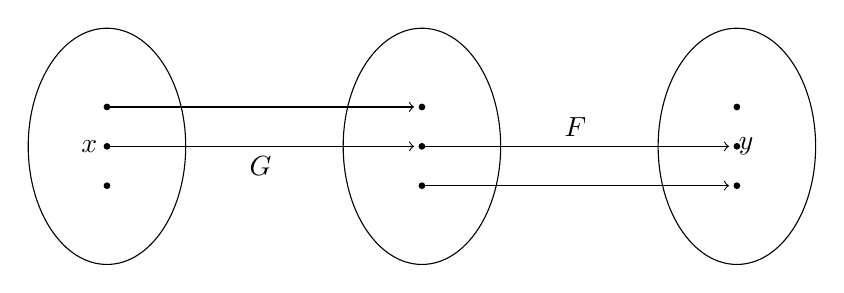
\begin{tikzpicture}
                        \draw (-4,0) ellipse [x radius = 1,y radius = 1.5];
                        \draw (0,0) ellipse [x radius = 1,y radius = 1.5];
                        \draw (4,0) ellipse [x radius = 1,y radius = 1.5];
                        \foreach \xOffset in {-4,0,4}{
                            \foreach \yOffset in {0.5,0,-0.5}{
                                \tikzPlaceDot{(\xOffset,\yOffset)};
                              }
                          }
                        \draw[->] (-4,0.5) -- (-0.1,0.5);
                        \draw[->] (-4,0) node[left]{$x$} --node[below]{$G$} (-0.1,0);
                        \draw[->] (0,0) --node[above]{$F$} (3.9,0) node[right]{$y$};
                        \draw[->] (0,-0.5) -- (3.9,-0.5);
                      \end{tikzpicture}
                    \end{center}

                    关于合成,还分为 :

                    \begin{itemize}
                      \item 顺序合成(右合成) : $F \circ G = \set{\dependent{x,y} | \exists z (xFz \land zGy)}$
                      \item 逆序合成(左合成) : $F \circ G = \set{\dependent{x,y} | \exists z (xGz \land zFy)}$
                    \end{itemize}

                    合成运算有结合律 :

                    \begin{itemize}
                      \item 设$R_1,R_2,R_3$为集合,则 : $$
                              (R_1 \circ R_2) \circ R_3 = R_1 \circ (R_2 \circ R_3)
                            $$
                    \end{itemize}

                    证明 : \begin{math}
                      \forall\dependent{x,y}, \dependent{x,y} \in (R_1 \circ R_2) \circ R_3 \\
                      \Leftrightarrow \exists z (x R_3 z \land z(R_1 \circ R_2)y) \\
                      \Leftrightarrow \exists z (x R_3 z \land \exists t(z R_2 t \land t R_1 y)) \\
                      \Leftrightarrow \exists z \exists t(x R_3 z \land (z R_2 t \land t R_1 y)) \\
                      \Leftrightarrow \exists t \exists z(x R_3 z \land z R_2 t \land t R_1 y) \\
                      \Leftrightarrow \exists t \exists z (x R_3 z \land z R_2 t \land t R_1 y) \\
                      \Leftrightarrow \exists t(\exists z(x R_3 z \land z R_2 t) \land t R_1 y) \\
                      \Leftrightarrow \exists t(x(R_2 \circ R_3)t \land t R_1 y) \\
                      \Leftrightarrow x R_1 \circ (R_2 \circ R_3) y \\
                      \Leftrightarrow \dependent{x,y} \in R_1 \circ (R_2 \circ R_3) \\
                      \therefore (R_1 \circ R_2) \circ R_3 = R_1 \circ (R_2 \circ R_3)
                    \end{math}

                    \qed
                    }
            \end{itemize}
            }
      \item {
            对任意集合$F,A$,可以定义 :

            \begin{itemize}
              \item 限制(restriction) : $F \upharpoonright  A = \set{\dependent{x,y} | xFy \land x \in A}$
              \item 象(image) : $F[A] = ran(F \upharpoonright A),F[A] = \set{y | \exists x (x \in A \land xFy)}$
            \end{itemize}
            }
      \item {
            对任意集合$F$,可以定义 :

            \begin{itemize}
              \item {
                    单根(single rooted) : 一个$y$对应唯一的一个$x$就是单根.

                    $F$是单根的 $\Leftrightarrow \forall y(y \in ran\ F \to \exists! x(x \in dom\ F \land xFy)) \Leftrightarrow (\forall y \in ran\ F)(\exists! x \in dom\ F)(xFy)$

                    \begin{itemize}
                      \item $\exists!$表示"存在唯一的"
                      \item $\forall x (x \in A \to B(x))$缩写为$(\forall x \in A)B(x)$
                      \item $\exists x (x \in A \land B(x))$缩写为$(\exists x \in A)B(x)$
                    \end{itemize}
                    }
              \item {
                    单值(single valued) : 一个$x$对应一个唯一的$y$就是单值.
                    $$
                      \mbox{$F$是单值的} \Leftrightarrow \forall x(x \in dom\ F \to \exists! y (y \in \rangle F \land xFy)) \Leftrightarrow (\forall x \in dom\ F)(\exists! y \in ran\ F)(xFy)
                    $$
                    }
            \end{itemize}
            }
    \end{itemize}
  }%与二元关系有关的概念结尾

}%二元关系结尾

\subsection{关系的表示与性质}{

  \subsubsection{关系矩阵}{
    设$A = \set{a_1,a_2,...,a_n},R \subseteq A \times A$

    $R$的关系矩阵为一个$n \times n$的方阵$M(R) = (r_{ij})_{n \times n}$ : $$
      M(R)(i,j) = r_{ij} = \begin{cases}
        1,\ a_iRa_j \\
        0,\ \mbox{否则}
      \end{cases}
    $$

    举个例子 : \begin{itemize}
      \item $A = \set{a,b,c}$
      \item $R_1 = \set{\dependent{a,a},\dependent{a,b},\dependent{b,a},\dependent{b,c}}$
      \item $R_2 = \set{\dependent{a,b},\dependent{a,c},\dependent{b,c}}$
    \end{itemize}

    $$
      M(R_1) = \begin{bmatrix}
        1 & 1 & 0 \\
        1 & 0 & 1 \\
        0 & 0 & 0
      \end{bmatrix}
      \qquad
      M(R_2) = \begin{bmatrix}
        0 & 1 & 1 \\
        0 & 0 & 1 \\
        0 & 0 & 0
      \end{bmatrix}
    $$

    注 : 默认从左到右,从上到下按$a,b,c$的顺序排列.
  }%关系矩阵结尾

  \subsubsection{关系矩阵的性质}{
    \begin{itemize}
      \item 集合表达式与关系矩阵可以唯一互相确定
      \item $M(R\inverse) = (M(R))\transpose$\begin{itemize}
              \item $~\transpose$表示矩阵转置
            \end{itemize}
      \item $M(R_1 \circ R_2) = M(R_2) \cdot M(R_1)$\begin{itemize}
              \item $\cdot$表示矩阵的"逻辑乘"(即分量相加或数乘换成逻辑操作),加法用$\lor$,乘法用$\land$
            \end{itemize}
    \end{itemize}
  }%关系矩阵的性质结尾

  \subsubsection{关系矩阵举例}{
    \begin{itemize}
      \item $A = \set{a,b,v}$
      \item $R_1 = \set{\dependent{a,a},\dependent{a,b},\dependent{b,a},\dependent{b,c}}$
      \item $R_2 = \set{\dependent{a,b},\dependent{a,c},\dependent{b,c}}$
      \item 用$M(R_1),M(R_2)$确定$M(R_1\inverse),M(R_2\inverse),M(R_1 \circ R_1),M(R_1 \circ R_2)$,从而求出他们的集合表达式.
    \end{itemize}

    解 : $$
      M(R_1) = \begin{bmatrix}
        1 & 1 & 0 \\
        1 & 0 & 1 \\
        0 & 0 & 0
      \end{bmatrix},\qquad
      M(R_2) = \begin{bmatrix}
        0 & 1 & 1 \\
        0 & 0 & 1 \\
        0 & 0 & 0
      \end{bmatrix},\qquad
      M(R_1\inverse) = \begin{bmatrix}
        1 & 1 & 0 \\
        1 & 0 & 0 \\
        0 & 1 & 0
      \end{bmatrix},\qquad
      M(R_2\inverse) = \begin{bmatrix}
        0 & 0 & 0 \\
        1 & 0 & 0 \\
        1 & 1 & 0
      \end{bmatrix}
    $$
    \begin{itemize}
      \item $R_1\inverse = \set{\dependent{a,a},\dependent{a,b},\dependent{b,a},\dependent{c,b}}$
      \item $R_2\inverse = \set{\dependent{b,a},\dependent{c,a},\dependent{c,b}}$
    \end{itemize}
    $$
      M(R_1 \circ R_1) = \begin{bmatrix}
        1 & 1 & 0 \\
        1 & 0 & 1 \\
        0 & 0 & 0
      \end{bmatrix}
      \cdot
      \begin{bmatrix}
        1 & 1 & 0 \\
        1 & 0 & 1 \\
        0 & 0 & 0
      \end{bmatrix}
      =
      \begin{bmatrix}
        1 & 1 & 1 \\
        1 & 1 & 0 \\
        0 & 0 & 0
      \end{bmatrix}
    $$
    \begin{itemize}
      \item $R_1 \circ R_1 = \set{\dependent{a,a},\dependent{a,b},\dependent{a,c},\dependent{b,a},\dependent{b,b}}$
    \end{itemize}
    $$
      M(R_1 \circ R_2) = \begin{bmatrix}
        0 & 1 & 1 \\
        0 & 0 & 1 \\
        0 & 0 & 0
      \end{bmatrix}
      \cdot
      \begin{bmatrix}
        1 & 1 & 0 \\
        1 & 0 & 1 \\
        0 & 0 & 0
      \end{bmatrix}
      =
      \begin{bmatrix}
        1 & 0 & 1 \\
        0 & 0 & 0 \\
        0 & 0 & 0
      \end{bmatrix}
    $$
    \begin{itemize}
      \item $R_1 \circ R_2 = \set{\dependent{a,a},\dependent{a,c}}$
    \end{itemize}
  }%关系矩阵举例结尾

  \subsubsection{关系图}{
    \begin{itemize}
      \item $A = \set{a_1,a_2,\dots,a_n},R \subseteq A \times A$
      \item {
            $R$的关系图$G(R)$ : \begin{itemize}
              \item 以"$o$"表示$A$中元素(称为顶点), 以"$\rightarrow$"表示$R$中元素(称为有向边)
              \item 若$a_iRa_j$,则从顶点$a_i$向顶点$a_j$引有向边$\dependent{a_i,a_j}$
            \end{itemize}
            }
    \end{itemize}
  }%关系图结尾

  \subsubsection{关系图举例}{
    \begin{itemize}
      \item $A = \set{a,b,c}$
      \item $R_1 = \set{\dependent{a,a},\dependent{a,b},\dependent{b,a},\dependent{b,c}}$
      \item $R_2 = \set{\dependent{a,b},\dependent{a,c},\dependent{b,c}}$
      \item $R_1\inverse = \set{\dependent{a,a},\dependent{a,b},\dependent{b,a},\dependent{c,b}}$
      \item $R_2\inverse = \set{\dependent{b,a},\dependent{c,a},\dependent{c,b}}$
      \item $R_1 \circ R_1 = \set{\dependent{a,a},\dependent{a,b},\dependent{a,c},\dependent{b,a},\dependent{b,b}}$
      \item $R_1 \circ R_1 = \set{\dependent{a,a},\dependent{a,c}}$
      \item $R_2 \circ R_1 = \set{\dependent{a,b},\dependent{a,c},\dependent{b,b},\dependent{b,c}}$
    \end{itemize}
    \begin{center}
      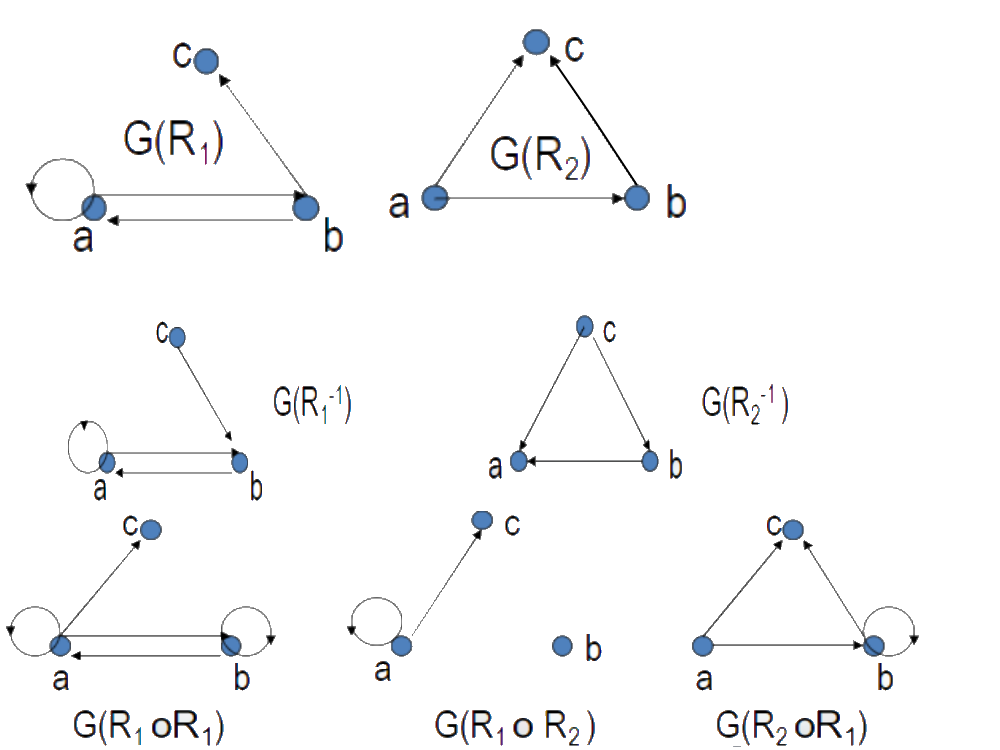
\includegraphics[scale=0.5]{resources/dependGraphic_1.png}

      去他妈的tikz!
    \end{center}
  }%关系图举例

  \subsubsection{讨论}{
    \begin{itemize}
      \item 当$A$中元素标定次序后,对于$R \subseteq A \times A$ : \begin{itemize}
              \item $G(R)$与$R$的集合表达式可唯一互相确定.
              \item $R$的集合表达式,关系矩阵,关系图三者均可唯一互相确定.
            \end{itemize}
      \item 对于$R \subseteq A \times B$ : \begin{itemize}
              \item $\absoluteValue{A} = n,\absoluteValue{B} = m$,关系矩阵$M(R)$时$n \times m$阶.
              \item $G(R)$中边都是从$A$中元素指向$B$中元素.
            \end{itemize}
    \end{itemize}
  }%讨论结尾

  \subsubsection{关系的性质}{
    \begin{itemize}
      \item {
            自反性(reflexivity) : \begin{itemize}
              \item $R \subseteq A \times A$
              \item $R$是自反的$\Leftrightarrow \forall x(x \in A \to xRx) \Leftrightarrow (\forall x \in A)xRx$
              \item $R$是非自反的$\Leftrightarrow \exists x (x \in A \land \lnot xRx)$
            \end{itemize}

            \begin{center}
              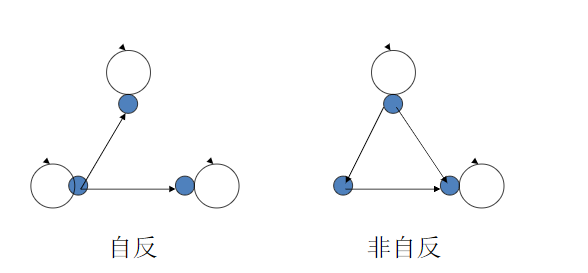
\includegraphics{resources/reflexivity.png}
            \end{center}

            定理 : 以下描述等价
            \begin{itemize}
              \item $R$是自反的
              \item $I_A \subseteq R$
              \item $R\inverse$是自反的
              \item $M(R)$主对角线上的元素全为$1$
              \item $G(R)$的每个顶点处均有环.
            \end{itemize}
            }
      \item {
            反自反性(irreflexivity) : \begin{itemize}
              \item $R \subseteq A \times A$
              \item $R$是反自反的$\Leftrightarrow \forall x(x \in A \to \lnot xRx) \Leftrightarrow (\forall x \in A)\lnot xRx$
              \item $R$是非反自反的$\Leftrightarrow \exists x(x \in A \land xRx)$
            \end{itemize}

            \begin{center}
              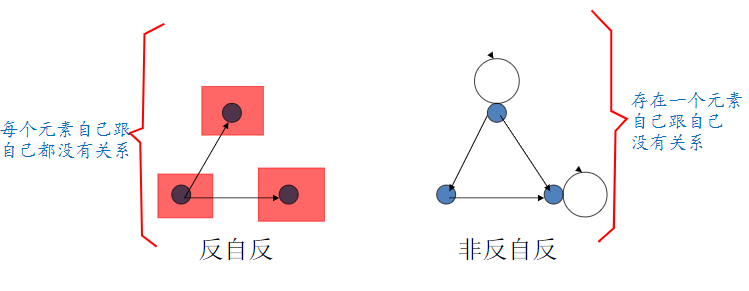
\includegraphics{resources/irreflexivity.png}
            \end{center}

            定理 : 以下描述等价
            \begin{itemize}
              \item $R$是反自反的
              \item $I_A \intersectionSet R = \emptyset$
              \item $R\inverse$是反自反的
              \item $M(R)$主对角线上的元素全为0
              \item $G(R)$的每个顶点处均无环.
            \end{itemize}

            自反且反自反 : $\emptyset$上的空关系
            }
      \item {
            对称性(symmetry) : \begin{itemize}
              \item $R \subseteq A \times A$
              \item $R$是对称的$\Leftrightarrow \forall x \forall y (x \in A \land y \in A \land xRy \to yRx) \Leftrightarrow (\forall x \in A)(\forall y \in A)[xRy \to yRx]$
              \item $R$是非对称的$\Leftrightarrow \exists x \exists y(x \in A \land y \in A \land xRy \land \lnot yRx)$
            \end{itemize}

            \begin{center}
              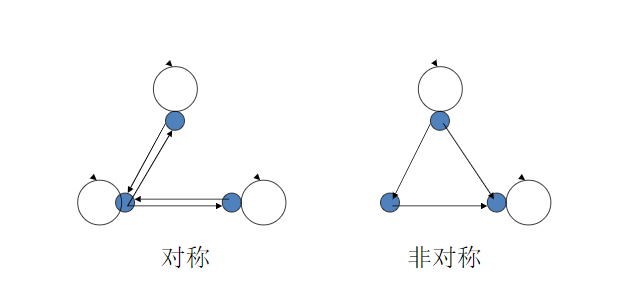
\includegraphics{resources/symmetry.png}
            \end{center}

            定理 : 以下描述等价
            \begin{itemize}
              \item $R$是对称的
              \item $R\inverse = R$
              \item $R\inverse$是对称的
              \item $G(R)$的任何两个顶点之间若有边,则必有两条方向相反的有向边.
            \end{itemize}
            }
      \item {
            反对称性(antisymmetry) : \begin{itemize}
              \item $R \subseteq A \times A$
              \item $R$是反对称的$\Leftrightarrow \forall x \forall y(x \in A \land y \in A \land xRy \land yRx \to x = y) \Leftrightarrow (\forall x \in A)(\forall y \in A)[xRy \land yRx \to x = y]$
              \item $R$非反对称$\Leftrightarrow \exists x \exists y (x \in A \land y \in A \land xRy \land yRx \land x \neq y)$
            \end{itemize}

            \begin{center}
              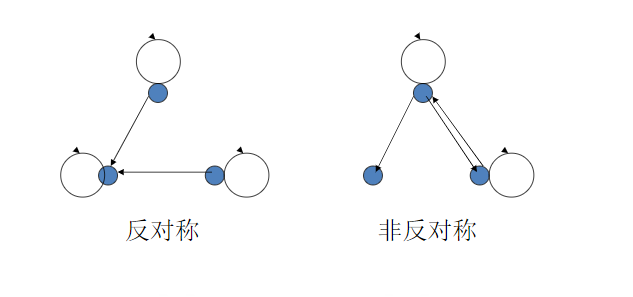
\includegraphics{resources/antisymmetry.png}
            \end{center}

            定理 : 以下叙述等价
            \begin{itemize}
              \item $R$是反对称的
              \item $R\inverse \intersectionSet R \subseteq I_A$
              \item $R\inverse$是反对称的
              \item 在$M(R)$中,$\forall i \forall j(i \neq j \land r_{ij} = 1 \to r_{ji} = 0)$
              \item 在$G(R)$中,$\forall a_i \forall a_j (i \neq j)$,若有有向边$\dependent{a_i,a_j}$,则必没有$\dependent{a_j,a_i}$.
            \end{itemize}
            }
      \item {
            传递性(transivity) : \begin{itemize}
              \item $R \subseteq A \times A$
              \item $R$是传递的$\Leftrightarrow \forall x \forall y \forall z (x \in A \land y \in A \land z \in A \land xRy \land yRz \to xRz)\Leftrightarrow(\forall x \in A)(\forall y \in A)(\forall z \in A)[xRy \land yRz \to xRz]$
              \item $R$非传递$\Leftrightarrow \exists x \exists y \exists z (x \in A \land y \in A \land z \in A \land xRy \land yRz \land \lnot xRz)$
            \end{itemize}

            \begin{center}
              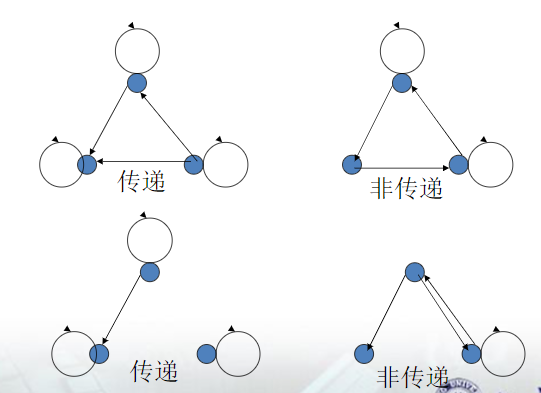
\includegraphics{resources/transivity.png}
            \end{center}

            定理 : 以下叙述等价
            \begin{itemize}
              \item $R$是传递的
              \item $R \circ R \subseteq R \Leftrightarrow R\inverse$是传递的
              \item $\forall i \forall j,M(R \circ R)(i,j) \leq M(R)(i,j)$
              \item 在$G(R)$中,$\forall a_i \forall a_j \forall a_k$,若有有向边$\dependent{a_i,a_j}$和$\dependent{a_j,a_k}$,则必有有向边$\dependent{a_i,a_k}$
            \end{itemize}
            }
    \end{itemize}

    在$\mathNatureNumberCollection = \set{0,1,2,...}$上 : \begin{itemize}
      \item $\leq = \set{\dependent{x,y} | x \in \mathNatureNumberCollection \land y \in \mathNatureNumberCollection \land x \leq y}$自反,反对称,传递
      \item $\geq = \set{\dependent{x,y} | x \in \mathNatureNumberCollection \land y \in \mathNatureNumberCollection \land x \geq y}$自反,反对称,传递
      \item $< = \set{\dependent{x,y} | x \in \mathNatureNumberCollection \land y \in \mathNatureNumberCollection \land x < y}$反自反,反对称,传递
      \item $> = \set{\dependent{x,y} | x \in \mathNatureNumberCollection \land y \in \mathNatureNumberCollection \land x > y}$反自反,反对称,传递
      \item $| = \set{\dependent{x,y} | x \in \mathNatureNumberCollection \land y \in \mathNatureNumberCollection \land x | y}$反对称,传递($\lnot 0 | 0$)
      \item $I_N = \set{\dependent{x,y} | x \in \mathNatureNumberCollection \land y \in \mathNatureNumberCollection \land x = y}$自反,对称,反对称,传递
      \item $E_N = \set{\dependent{x,y} | x \in \mathNatureNumberCollection \land y \in \mathNatureNumberCollection} = \mathNatureNumberCollection \times \mathNatureNumberCollection$自反,对称,传递
    \end{itemize}
  }%关系的性质结尾

}%关系的表示与性质结尾

\subsection{关系的幂运算和闭包}{

  \subsubsection{关系的n次幂}{
    \begin{itemize}
      \item {
            $R \subseteq A \times A,n \in \mathNatureNumberCollection$

            $$
              \begin{cases}
                R^0 = I_A \\
                R^{n + 1} = R^n \circ R\ (n \geq 0)
              \end{cases}
            $$
            }
      \item {
            显然$R^n \subseteq A \times A,n \in \mathNatureNumberCollection$
            }
    \end{itemize}

    $$
      R^n = R \circ R \circ \dots \circ R\qquad(n\mbox{个}R)
    $$

  }%关系的n次幂结尾

  \subsubsection{关系的幂运算的一些定理}{
    设$R \subseteq A \times A,m,n \in \mathNatureNumberCollection$,则 : \begin{enumerate}
      \item $R^m \circ R^n = R^{m + n}$
      \item $(R^m)^n = R^{mn}$
    \end{enumerate}

    \begin{proof}
      \begin{enumerate}
        \item {
              给定$m$,对$n$归纳 : $n = 0$时 : $$
                R^m \circ R^n = R^m \circ R^0 = R^m \circ I_A = R^m = R^{m + 0}
              $$

              假设$R^m \circ R^n = R^{m + n}$,则 :
              \begin{math}
                R^m \circ R^{n + 1} \\
                = R^m \circ (R^n \circ R^1) \\
                = (R^m \circ R^n) \circ R^1 \\
                = R^{m + n} \circ R \\
                = R^{(m + n) + 1} \\
                = R^{m + (n + 1)}
              \end{math}
              }
        \item 可类似证明.
      \end{enumerate}
    \end{proof}

    一言以蔽之,指数律对关系的幂运算也成立.
  }%关系的幂运算的一些定理结尾

  \subsubsection{幂运算举例}{
    尚未参透tikz怎么玩,就先拿ppt糊一下.

    \begin{center}
      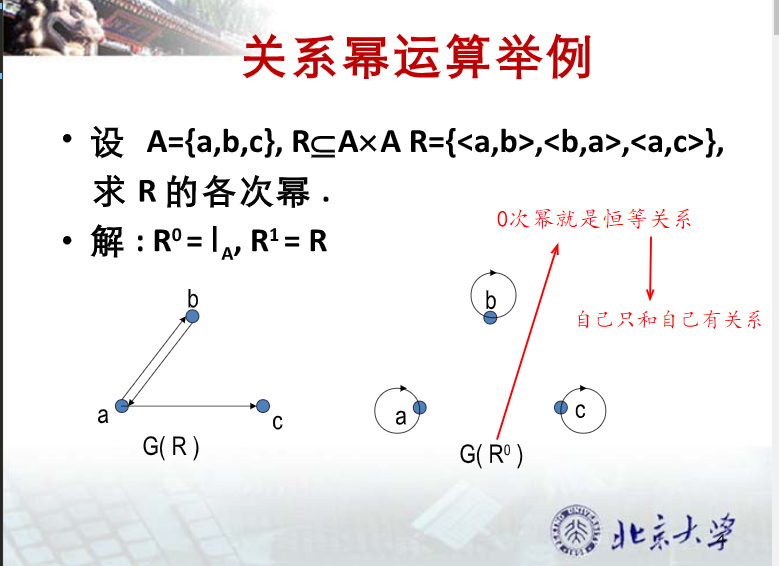
\includegraphics{resources/depend_power_example_1.png}
      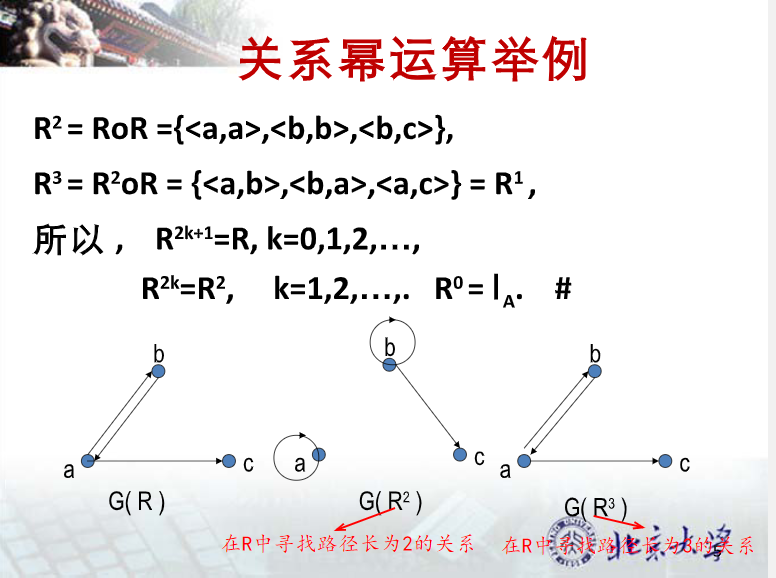
\includegraphics{resources/depend_power_example.png}
    \end{center}
  }

  思考:这好像和隔壁教线代的GS老爷子的骚操作有点关系...
}%关系的幂运算和闭包结尾

\subsubsection{关系的闭包}{
  在数学上,闭包的定义一般指的是这个意思 : 包含给定的一些元素,并且具有某种指定性质的最小集合称为 : 某些元素具有某性质的闭包.

  所以闭包一般有三个性质 : \begin{enumerate}
    \item 包含给定的元素
    \item 具有给定的性质
    \item 是最小的二元关系
  \end{enumerate}

  其中关系的闭包主要有以下三种 :

  \begin{itemize}
    \item 自反闭包$r(R)$ : 包含$R$,向$R$中加一些元素,使$R$自反.
    \item 对称闭包$s(R)$ : 包含$R$,并且使$R$对称.
    \item 传递闭包$t(R)$ : 包含$R$,并且使$R$构成传递的二元关系.
  \end{itemize}
}%关系的闭包

\subsubsection{自反闭包}{
  自反闭包$r(R)$有以下性质(定义也如下) : \begin{enumerate}
    \item $R \subseteq r(R)$
    \item $r(R)$是自反的
    \item $\forall s ((R \subseteq S \land S\mbox{自反}) \to r(R) \subseteq S)$ 注 : 此条是所谓"最小的"的其中一种定义.
  \end{enumerate}

  \begin{center}
    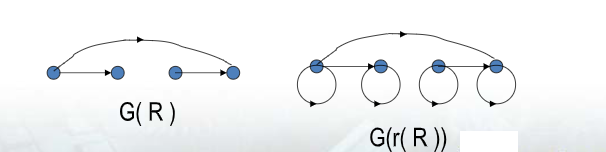
\includegraphics{resources/Reflexive_closure.png}
  \end{center}
}%自反闭包结尾

\subsubsection{对称闭包}{
  对称闭包有以下性质(定义也如下) : \begin{enumerate}
    \item $R \subseteq s(R)$
    \item $s(R)$是对称的
    \item $\forall S ((R \subseteq S \land S\mbox{对称}) \to s(R) \subseteq S)$ 注 : 此条是所谓"最小的"的其中一种定义.
  \end{enumerate}

  \begin{center}
    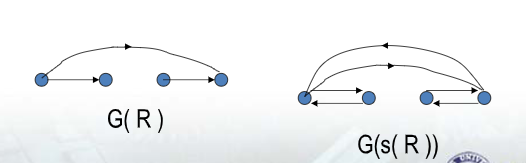
\includegraphics{resources/Symmetric_closure.png}
  \end{center}
}%对称闭包结尾

\subsubsection{传递闭包}{
  传递闭包有以下性质(定义也如下) : \begin{enumerate}
    \item $R \subseteq t(R)$
    \item $t(R)$是传递的
    \item $\forall S ((R \subseteq S \land S\mbox{传递}) \to t(R) \subseteq S)$ 注 : 此条是所谓"最小的"的其中一种定义.
  \end{enumerate}

  \begin{center}
    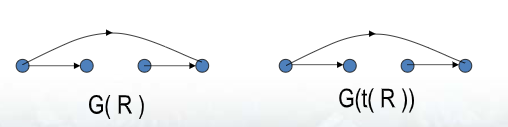
\includegraphics{resources/transivity_closure.png}
  \end{center}
}%传递闭包结尾

\subsubsection{关于闭包的一些定理}{
  \begin{enumerate}
    \item {
          设$R \subseteq A \times A$且$A \neq \emptyset$,则 : \begin{enumerate}
            \item $R$自反$\Leftrightarrow r(R) = R$
            \item $R$对称$\Leftrightarrow s(R) = R$
            \item $R$传递$\Leftrightarrow t(R) = R$
          \end{enumerate}
          }
    \item {
          设$R_1 \subseteq R_2 \subseteq A \times A$且$A \neq \emptyset$,则 : \begin{enumerate}
            \item $r(R_1) \subseteq r(R_2)$
            \item $s(R_1) \subseteq s(R_2)$
            \item $t(R_1) \subseteq t(R_2)$
          \end{enumerate}
          }
    \item {
          设$R_1,R_2\subseteq A \times A$且$A \neq \emptyset$,则 : \begin{enumerate}
            \item $r(R_1 \unionSet R_2) = r(R_1) \unionSet r(R_2)$
            \item $s(R_1 \unionSet R_2) = s(R_1) \unionSet s(R_2)$
            \item $t(R_1 \unionSet R_2) \supseteq t(R_1) \unionSet t(R_2)$
          \end{enumerate}
          \begin{proof}
            如下 :

            \begin{enumerate}
              \item {
                    $R_1 \unionSet R_2 \subseteq r(R_1) \unionSet r(R_2) \subseteq r(R_1 \unionSet R_2)$

                    又由$r(R_1) \unionSet r(R_2)$自反,所以$r(R_1 \unionSet R_2) \subseteq r(R_1) \unionSet r(R_2)$
                    }
              \item 可类似证明
              \item $t(R_1) \unionSet t(R_2) \subseteq t(R_1 \unionSet R_2)$
            \end{enumerate}
          \end{proof}
          注 : $t(R_1) \unionSet t(R_2)$不一定传递,反例如下 :

          \begin{center}
            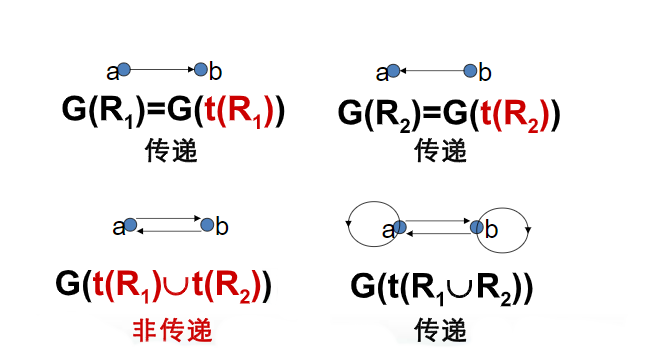
\includegraphics{resources/transivity_closure_2.png}
          \end{center}
          }
  \end{enumerate}
}%关于闭包的一些定理结尾

\subsubsection{闭包的求法}{
  \begin{itemize}
    \item 设$R \subseteq A \times A$且$A \neq \emptyset$,则 : \begin{itemize}
            \item $r(R) = R \unionSet I_A$(图形表示就是给每个点加上环)
            \item $s(R) = R \unionSet R\inverse$(图形表示就是给每个边加上反向的边)
            \item $t(R) = R \unionSet R^2 \unionSet R^3 \unionSet \dots$(传递闭包)
          \end{itemize}
    \item 对比 : \begin{itemize}
            \item $R$自反$\Leftrightarrow I_A \subseteq R$
            \item $R$对称$\Leftrightarrow R = R\inverse$
            \item $R$传递$\Leftrightarrow R^2 \subseteq R$
          \end{itemize}
  \end{itemize}

  \begin{proof}
    设$R \subseteq A \times A$且$A \neq \emptyset$,则 : \begin{itemize}
      \item {
            $r(R) = R \unionSet I_A$

            证明如下 :\begin{enumerate}
              \item $R \subseteq R \unionSet I_A$
              \item $I_A \subseteq R \unionSet I_A \Leftrightarrow R \unionSet I_A$自反$\Rightarrow r(R) \subseteq R \unionSet I_A$
              \item $R \subseteq r(R) \land r(R)$自反$\Rightarrow R \subseteq r(R) \land I_A \subseteq r(R) \Rightarrow R \unionSet I_A \subseteq r(R)$
            \end{enumerate}
            }
      \item {
            $s(R) = R \unionSet R\inverse$

            证明如下 : \begin{enumerate}
              \item $R \subseteq R \unionSet R\inverse$
              \item $(R \unionSet R\inverse)\inverse = R \unionSet R\inverse \Leftarrow R \unionSet R\inverse$对称$\Rightarrow s(R) \subseteq R \unionSet R\inverse$
              \item $R \subseteq s(R) \land R\inverse \subseteq s(R) \Rightarrow R \unionSet R\inverse \subseteq s(R)$
            \end{enumerate}
            }
      \item {
            $t(R) = R \unionSet R^2 \unionSet R^3 \unionSet \dots$

            证明如下 : \begin{enumerate}
              \item $R \subseteq R \unionSet R^2 \unionSet R^3 \unionSet \dots$
              \item {
                    \begin{itemize}
                      \item[] $(R \unionSet R^2 \unionSet R^3 \unionSet \dots)^2$
                      \item[$=$] $R^2 \unionSet R^3 \unionSet \dots \subseteq R \unionSet R^2 \unionSet R^3 \unionSet \dots$
                      \item[$\Leftrightarrow$]这玩意传递
                      \item[$\Rightarrow$] $t(R) \subseteq R \unionSet R^2 \unionSet R^3 \unionSet \dots$
                    \end{itemize}
                    }
              \item {
                    \begin{itemize}
                      \item[] $R \subseteq t(R) \land t(R)$传递
                      \item[$\Rightarrow$] $R \subseteq t(R) \land R^2 \subseteq t(R) \land R^3 \subseteq t(R) \land \dots$
                      \item[$\Rightarrow$] $R \unionSet R^2 \unionSet R^3 \unionSet \dots \unionSet \subseteq t(R)$
                    \end{itemize}

                    推论 : 设$R \subseteq A \times A$且$0 < \absoluteValue{A} < \absoluteValue{\infty}$,则$\exists I \in \mathNatureNumberCollection$,使得$t(R) = R \unionSet R^2 \unionSet R^3 \unionSet \dots \unionSet R^I$
                    }
            \end{enumerate}
            }
    \end{itemize}
  \end{proof}
}%闭包的求法结尾

\subsubsection{闭包运算与关系性质}{
  下表表示闭包运算后原本的关系的性质是否保持 :

  \begin{center}
    \begin{tabular}{|c|c|c|c|}
      \hline
      ~      & 自反性 & 对称性 & 传递性 \\
      \hline
      $r(R)$ & yes    & yes    & yes    \\
      \hline
      $s(R)$ & yes    & yes    & no     \\
      \hline
      $t(R)$ & yes    & yes    & yes    \\
      \hline
    \end{tabular}
  \end{center}

  以下为证明 :

  \begin{enumerate}
    \item {
          \begin{proof}
            $R$自反$\Rightarrow s(R)$和$t(R)$自反

            \begin{itemize}
              \item $I_A \subseteq R \unionSet R\inverse = s(R) \Rightarrow s(R)$自反
              \item $I_A \subseteq R \unionSet R^2 \unionSet R^3 \unionSet \dots t(R) \Rightarrow t(R)$自反
            \end{itemize}
          \end{proof}
          }
    \item {
          \begin{proof}
            $R$对称$\Rightarrow r(R)$和$t(R)$对称

            \begin{itemize}
              \item $r(R)\inverse = (I_A \unionSet R)\inverse = I_A\inverse \unionSet R\inverse = I_A \unionSet R\inverse = I_A \unionSet R = r(R) \Rightarrow r(R)$对称.
              \item {
                    \begin{itemize}
                      \item[] $t(R)\inverse = (R \unionSet R^2 \unionSet R^3 \unionSet \dots)\inverse$
                      \item[$=$] $R\inverse \unionSet (R^2)\inverse \unionSet (R^3)\inverse \unionSet \dots$
                      \item[$=$] $R\inverse \unionSet (R\inverse)^2 \unionSet (R\inverse)^3 \unionSet \dots$
                      \item[$=$] $R \unionSet R^2 \unionSet R^3 \unionSet \dots$
                      \item[$=$] $t(R)$
                      \item[$\Rightarrow$] $t(R)$对称.
                    \end{itemize}
                    }
            \end{itemize}
          \end{proof}
          }
    \item {
          \begin{proof}
            $R$传递$\Rightarrow r(R)$传递

            \begin{itemize}
              \item[] $r(R) \circ r(R) = (I_A \unionSet R) \circ (I_A \unionSet R)$
              \item[$=$] $(I_A \circ I_A) \unionSet (I_A \circ R) \unionSet (R \circ I_A) \unionSet (R \circ R)$
              \item[$\subseteq$] $I_A \unionSet R \unionSet R \unionSet R = I_A \unionSet R = r(R)$
              \item[$\Rightarrow$] $r(R)$传递.
            \end{itemize}
          \end{proof}

          注 : $R$传递$ \nRightarrow s(R)$传递,反例 :
          \begin{center}
            \begin{tikzpicture}
              \tikzPlaceNode{a}{(-1,0)}{~};
              \tikzPlaceNode{b}{(1,0)}{~};
              \draw[very thick,->] (a) -- (b);
            \end{tikzpicture}
            \begin{tikzpicture}
              \tikzPlaceNode{a}{(-1,0)}{~};
              \tikzPlaceNode{b}{(1,0)}{~};
              \tikzPlaceShiftLeftRightArrow{a}{b}
            \end{tikzpicture}

            $H(R)$ \qquad $G(s(R))$
          \end{center}
          }
  \end{enumerate}
}%闭包运算与关系性质结尾

\subsubsection{闭包运算与关系性质相关定理}{
  \begin{itemize}
    \item {
          设$R \subseteq A \times A$且$A \neq \emptyset$,则 : \begin{enumerate}
            \item $rs(R) = sr(R)$
            \item $rt(R) = tr(R)$
            \item $st(R) = ts(R)$
          \end{enumerate}

          注 : $rs(R) = r(s(R))$

          证明 : \begin{enumerate}
            \item {
                  \begin{itemize}
                    \item[] $rs(R) = r(s(R) = r(R \unionSet R\inverse)) = I_A \unionSet (R \unionSet R\inverse)$
                    \item[$=$] $(I_A \unionSet R) \unionSet (I_A\inverse \unionSet R\inverse) = (I_A \unionSet r) \unionSet (I_A \unionSet R)\inverse$
                    \item[$=$] $r(R) \unionSet r(R)\inverse = s(r(R)) = sr(R)$
                  \end{itemize}
                  }
            \item {
                  \begin{itemize}
                    \item[] $rt(R) = r(t(R)) = r(R \unionSet R^2 \unionSet R^3 \unionSet \dots) = I_A \unionSet (R \unionSet R^2 \unionSet R^3 \unionSet \dots)$
                    \item[$=$] $(I_A \unionSet R)\unionSet(I_A \unionSet R \unionSet R^2) \unionSet (I_A \unionSet R \unionSet R^2 \unionSet R^3) \unionSet \dots$
                    \item[$=$] $(I_A \unionSet R) \unionSet (I_A \unionSet R)^2 \unionSet (I_A \unionSet R)^3 \unionSet \dots$
                    \item[$=$] $r(R) \unionSet r(R)^2 \unionSet r(R)^3 \unionSet \dots$
                    \item[$=$] $t(r(R)) = tr(R)$
                  \end{itemize}
                  }
            \item {
                  $st(R) \subseteq st(s(R)) = sts(R) = s(ts(R)) = ts(R)$

                  ($ts(R)$对称)

                  反例 : $st(R) \subset ts(R)$ :
                  }
          \end{enumerate}
          }
  \end{itemize}

  \begin{center}
    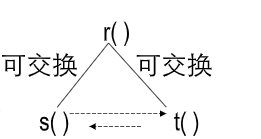
\includegraphics{resources/closure_properties_example_1.png}
  \end{center}
}%闭包运算与关系性质相关定理结尾

}%集合论结尾

\section{图论}{

  \subsection{图论的主要内容}{
    \begin{itemize}
      \item 研究对象 : 由顶点和边构成的图
      \item 研究思想 : 以集合论为基础,以图为工具,为各种二元关系建立模型
      \item 研究内容 : \begin{itemize}
              \item 图的基本概念 : 连通性,矩阵表示,带权图
              \item 欧拉图,哈密顿图 : 边和顶点的遍历
              \item 树 : 表示层级组织关系
              \item 平面图 : 判定,表示,性质
              \item 图的着色 : 各种调度问题的模型
              \item 独立集,支配集,覆盖集,匹配 : 各种应用问题
            \end{itemize}
    \end{itemize}
  }%图论的主要内容结尾

  \subsection{图论中的问题}{
    \begin{itemize}
      \item 什么是图?有哪些图?图有什么性质?
      \item 什么是欧拉图?什么是哈密顿图?
      \item 什么是树?如何用矩阵表示图?
      \item 什么是图的着色?
      \item 什么是支配集,独立集,覆盖,匹配?
      \item 什么是带权图?
    \end{itemize}
  }%图论中的问题结尾

 }%图论结尾

}%离散数学结尾
  %*近世代数
  % \chapter{抽象代数}{
    
}%抽象代数结尾
  %*数论
  % \section{数论}{

 }%数论结尾

 }%数学篇结尾
% #TODO ComputerScience
% \part{计算机科学}{

  %*计算机图形学
  % \section{计算机图形学}{
  注:本章中向量默认为列向量.

  \subsection{对于线性代数部分的补充与扩展}{

    在计算机图形学中线性代数的主要作用是操纵与计算空间中对象的变化.由此衍生出了一些特殊的观点.

    同时有一部分重要的常用基础内容放在了数学篇中的空间解析几何部分.

    \begin{enumerate}
      \item {向量叉乘的对偶矩阵:
            $$\vec{a} \times \vec{b}
              =
              \begin{bmatrix}
                y_az_b - y_bz_a \\
                z_ax_b - x_az_b \\
                x_ay_b - y_ax_b
              \end{bmatrix}
              =
              A * \vec{b}
              =
              \begin{bmatrix}
                0    & -z_a & y_a  \\
                z_a  & 0    & -x_a \\
                -y_a & x_a  & 0
              \end{bmatrix}
              \begin{bmatrix}
                x_b \\
                y_b \\
                z_b
              \end{bmatrix}
            $$
            }
      \item 非满秩矩阵意味着将空间变换到了更低的维度.
      \item 特征向量是指在进行了矩阵所代表的线性变换后方向没改变向量,特征值则是指特征向量的缩放倍数.
      \item 逆矩阵所代表的变换成为逆变换,是原矩阵所代表的变换的反向操作,一个矩阵乘以他的逆矩阵是单位阵,这从几何上的直观理解就是什么都没做,两次操作互相抵消了.
    \end{enumerate}
  }

  \subsection{变换}{
    变换按照作用对象可以分为:
    \begin{enumerate}
      \item Modeling 模型变换
      \item Viewing 视角变换
    \end{enumerate}

    按照作用效果可以分为:
    \begin{enumerate}
      \item scale 缩放变换
      \item rotate 旋转变换
      \item shear 剪切变换
    \end{enumerate}

    如同3b1b的观点,将目标空间看作矩阵的列空间.而矩阵每一列都对应了列空间中的一个基向量,拿2维空间举例:
    $$
      \begin{bmatrix}
        1 & 0 \\
        0 & 1
      \end{bmatrix}
    $$

    假设第一列代表了$x$轴的单位向量$i$,则第二列代表了$y$轴的单位向量$j$

    因此,对矩阵进行操作就相当于对矩阵所代表的空间进行操作.

    例如:$$
      \begin{bmatrix}
        2 & 1 \\
        1 & 2
      \end{bmatrix}
    $$

    这个矩阵就代表着将单位向量$i$移动到了坐标$(2,1)$,将单位向量$j$移动到了坐标$(1,2)$.整个二维空间都是由这两个单位向量所张成的.随着单位向量的移动,整个空间也就随之而变形.这种操作被称为变换.
    其中一类最简单的变换称为线性变换,在线性代数篇中已有了详细解释.

    旋转矩阵的表示原理如下:

    先看看二维:

    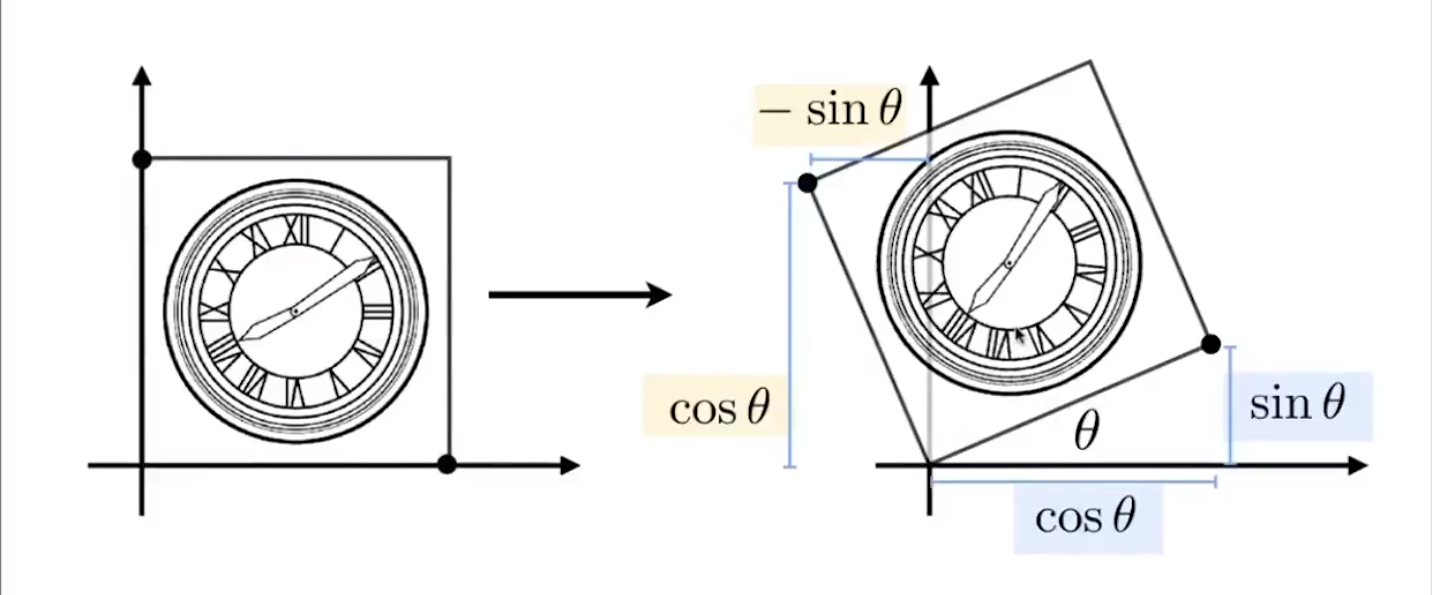
\includegraphics[scale=0.25]{resources/rotateMatrixGraphics.png}

    因此二维的旋转矩阵$$
      R_\theta = \begin{bmatrix}
        \cos\theta & -\sin\theta \\
        \sin\theta & \cos\theta
      \end{bmatrix}
    $$


    \subsubsection{齐次坐标}{
      由于单纯的线性变换并不能让对象动起来,依然只能在原点操作,所以需要齐次坐标表示空间上的位移.

      如下图:

      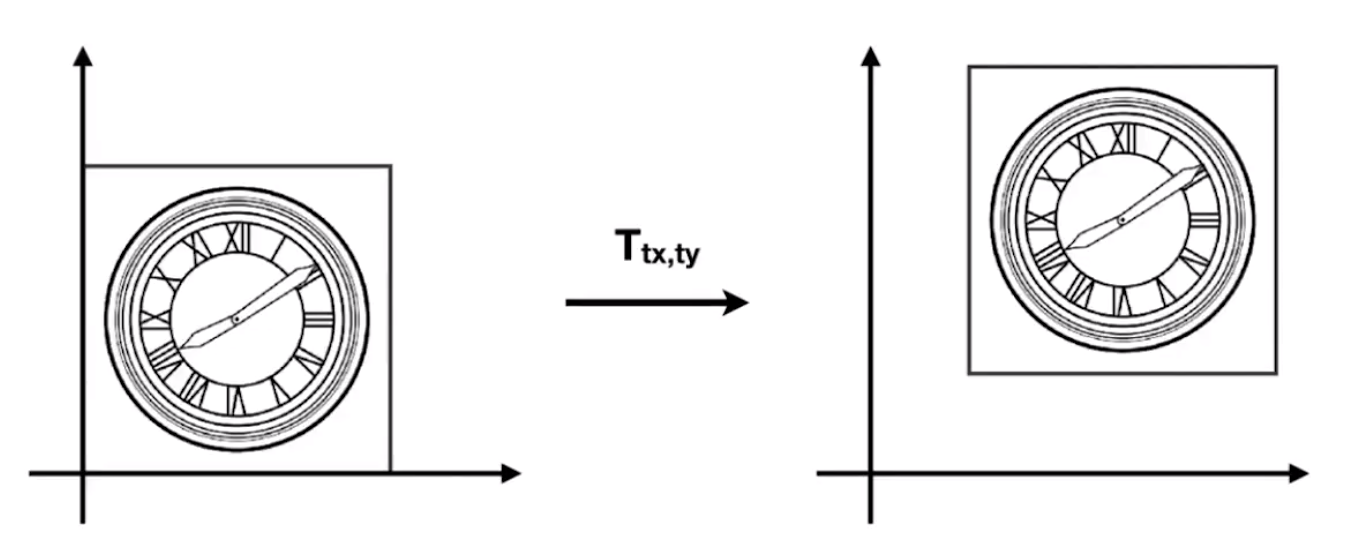
\includegraphics[scale=0.25]{resources/homogeneous_coordinates.png}

      用$x\prime$和$y\prime$来表示变换后的坐标,公式为:

      $x\prime = x + t_x$

      $y\prime = y + t_y$

      仔细思考一下发现似乎并不能写成矩阵$A\vec{x} = \vec{b}$的形式.

      事实上应该写成这样:
      $$
        \begin{bmatrix}
          x\prime \\
          y\prime
        \end{bmatrix}
        =
        \begin{bmatrix}
          a & b \\
          c & d
        \end{bmatrix}
        \begin{bmatrix}
          x \\
          y
        \end{bmatrix}
        +
        \begin{bmatrix}
          t_x \\
          t_y
        \end{bmatrix}
      $$

      因此平移变换不属于线性变换.但是人们不想要特殊情况,于是引入了齐次坐标:

      还是拿二维的情况举例,增加一个维度,将二维的点表示为:
      $$\begin{bmatrix}
          x & y & 1
        \end{bmatrix}^T$$

      将二维向量表示为:
      $$\begin{bmatrix}
          x & y & 0
        \end{bmatrix}^T$$

      也就是说:再多增加一个维度用于说明表示的是一个点还是一个向量,这是因为向量具有平移不变性,不管怎么移动表示的始终是一个方向.

      齐次坐标的好处就在这里,它是这么用的:

      $$\begin{bmatrix}
          x\prime \\
          y\prime \\
          w\prime
        \end{bmatrix}
        =
        \begin{bmatrix}
          1 & 0 & t_x \\
          0 & 1 & t_y \\
          0 & 0 & 1
        \end{bmatrix}
        \cdot
        \begin{bmatrix}
          x \\
          y \\
          1
        \end{bmatrix}
        =
        \begin{bmatrix}
          x + t_x \\
          y + t_y \\
          1
        \end{bmatrix}
      $$

      更直观一点:可以这么理解:
      \begin{itemize}
        \item 向量 + 向量 = 向量, 向量相加还是向量 $0 + 0 = 0$
        \item 点 - 点 = 向量, 两点相减得到向量 $1 - 1 = 0$
        \item 点 + 向量 = 点, 一个点加一个向量结果是一个点 $0 + 1 = 1$
        \item 点 + 点 = 两个点的中点, $1 + 1 = 2$,原因见扩充定义.
      \end{itemize}
      扩充定义如下:
      $$\begin{bmatrix}
          x \\
          y \\
          w
        \end{bmatrix} = \begin{bmatrix}
          x \\
          y \\
          w
        \end{bmatrix}\cdot\cfrac{1}{w} = \begin{bmatrix}
          \cfrac{x}{w} \\
          \cfrac{y}{w} \\
          1
        \end{bmatrix}$$

      {\bfseries于是总结,给出以下下定义:}\\\\\indent
      仿射变换(Affine transformation) = 线性变换(Linear transformation) + 位移(transformation)

      即:
      $$\begin{bmatrix}
          x\prime \\
          y\prime
        \end{bmatrix}
        =
        \begin{bmatrix}
          a & b \\
          c & d
        \end{bmatrix}
        \cdot
        \begin{bmatrix}
          x \\
          y
        \end{bmatrix}
        +
        \begin{bmatrix}
          t_x \\
          t_y
        \end{bmatrix}$$

      都可以写成齐次坐标(homogeneous coordinates)的形式

      即:
      $$\begin{bmatrix}
          x\prime \\
          y\prime \\
          1
        \end{bmatrix}
        =
        \begin{bmatrix}
          a & b & t_x \\
          c & d & t_y \\
          0 & 0 & 1
        \end{bmatrix}
        \cdot
        \begin{bmatrix}
          x \\
          y \\
          1
        \end{bmatrix}$$

      {\bfseries不如直接将其他操作的齐次坐标形式补全吧?}
      \begin{itemize}
        \item 缩放(scale) : $$S(s_x, s_y) = \begin{bmatrix}
                  s_x & 0   & 0 \\
                  0   & s_y & 0 \\
                  0   & 0   & 0
                \end{bmatrix}$$
        \item 旋转(rotation) : $$R(\alpha) = \begin{bmatrix}
                  \cos\alpha & -\sin\alpha & 0 \\
                  \sin\alpha & \cos\alpha  & 0 \\
                  0          & 0           & 1
                \end{bmatrix}$$
        \item 平移(translation) : $$T(t_x, t_y) = \begin{bmatrix}
                  1 & 0 & t_x \\
                  0 & 1 & t_y \\
                  0 & 0 & 1
                \end{bmatrix}$$
      \end{itemize}

    }%齐次坐标结尾

    \subsubsection{组合变换}{
      可以通过组合各个基础变换以形成复杂的变换效果.

      组合方法为对应矩阵按照顺序从右向左做乘法.

      大部分时候组合顺序至关重要.

    }%组合变换结尾

    \subsubsection{三维变换}{
      以上结论都可以用于三维,推而广之:\\

      齐次坐标:\begin{itemize}
        \item 三维点:$$\begin{bmatrix}
                  x \\
                  y \\
                  z \\
                  1
                \end{bmatrix}$$
        \item 三维向量:$$\begin{bmatrix}
                  x \\
                  y \\
                  z \\
                  0
                \end{bmatrix}$$
      \end{itemize}

      $\left[x\ y\ z\ w\right]^T$,当$w$不等于$1$他所表示的三维的点其实是(第四个维度已略去):
      $$\begin{bmatrix}
          \cfrac{x}{w} \\
          \cfrac{y}{w} \\
          \cfrac{z}{w} \\
        \end{bmatrix}$$

      同样的,三维空间中齐次坐标描述的仿射变换的矩阵是$4 \times 4$的:
      $$\begin{bmatrix}
          x\prime \\
          y\prime \\
          z\prime \\
          1
        \end{bmatrix}
        =
        \begin{bmatrix}
          a & b & c & t_x \\
          d & e & f & t_y \\
          g & h & i & t_z \\
          0 & 0 & 0 & 1
        \end{bmatrix}
        \cdot
        \begin{bmatrix}
          x \\
          y \\
          z \\
          1
        \end{bmatrix}$$

      将二维操作类比过来:

      \begin{itemize}
        \item 缩放 : $$
                S(s_x,s_y,s_z) =\begin{bmatrix}
                  s_x & 0   & 0   & 0 \\
                  0   & s_y & 0   & 0 \\
                  0   & 0   & s_z & 0 \\
                  0   & 0   & 0   & 1
                \end{bmatrix}
              $$
        \item 平移 : $$
                T(t_x,t_y,t_z) = \begin{bmatrix}
                  1 & 0 & 0 & t_x \\
                  0 & 1 & 0 & t_y \\
                  0 & 0 & 1 & t_z \\
                  0 & 0 & 0 & 1
                \end{bmatrix}
              $$
        \item 三维旋转(绕某个轴逆时针旋转) :
              $$
                R_x(\alpha) = \begin{bmatrix}
                  1 & 0          & 0           & 0 \\
                  0 & \cos\alpha & -\sin\alpha & 0 \\
                  0 & \sin\alpha & \cos\alpha  & 0 \\
                  0 & 0          & 0           & 1
                \end{bmatrix}
              $$

              $$
                R_y(\alpha) = \begin{bmatrix}
                  \cos\alpha  & 0 & \sin\alpha & 0 \\
                  0           & 1 & 0          & 0 \\
                  -\sin\alpha & 0 & \cos\alpha & 0 \\
                  0           & 0 & 0          & 1
                \end{bmatrix}
              $$

              $$
                R_z(\alpha) = \begin{bmatrix}
                  \cos\alpha & -\sin\alpha & 0 & 0 \\
                  \sin\alpha & \cos\alpha  & 0 & 0 \\
                  0          & 0           & 1 & 0 \\
                  0          & 0           & 0 & 1
                \end{bmatrix}
              $$
        \item 三维旋转(欧拉角) : $R_{xyz}(\alpha,\beta,\gamma) = R_x(\alpha)R_y(\beta)R_z(\gamma)$
        \item 三维旋转($\vec{I}$绕任意轴n旋转角度$\alpha$)(罗德里格斯旋转公式) : $$
                R(n,\alpha) = \cos(\alpha)\vec{I} + (1 - \cos(\alpha))\vec{n}\vec{n}\transpose + \sin(\alpha)\begin{bmatrix}
                  0    & -n_z & n_y  \\
                  n_z  & 0    & -n_x \\
                  -n_y & n_x  & 0
                \end{bmatrix}
              $$
              (其中$\vec{n}$为旋转轴的单位向量)
      \end{itemize}
    }%三维变换结尾

    \subsubsection{观测变换}{
      一般来说拍一张照片的步骤如下 :

      \begin{enumerate}
        \item 找到一个好的位置摆放人物(模型变换,model transformation)
        \item 找到一个好的"角度"来放下相机(视图变换,view transformation)
        \item 按下快门(投影变换,projection transformation)
      \end{enumerate}

      \begin{itemize}
        \item {
              视图变换(view transformation) :

              首先定义相机:
              \begin{itemize}
                \item 位置(Position) : $\vec{e}$
                \item 视线方向(Look-at/gaze direction) : $\hat{\vec{g}}$
                \item 向上方向(UP direction) : $\hat{\vec{t}}$ (注:这个表示的是相机自身的旋转,此向量垂直于上面两个向量张成的平面)
              \end{itemize}

              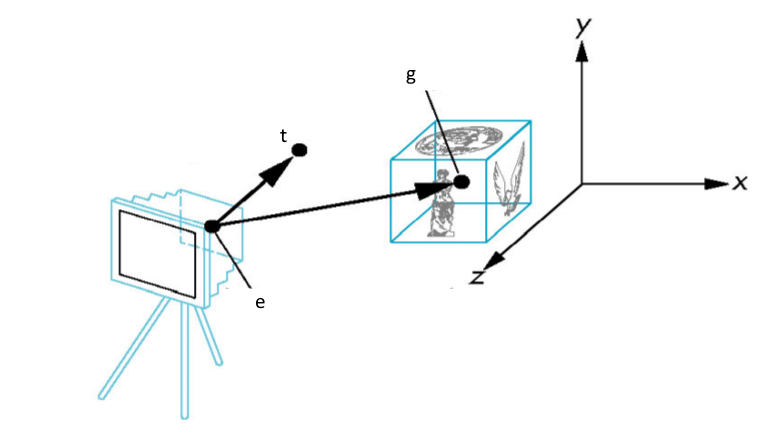
\includegraphics[scale=0.9]{resources/viewTransformation.png}

              值得注意的是: 定义相机永远在原点,视线朝向-z方向,以y轴作为向上方向(约定俗成,这么做有很多好处)

              所以在实际情况中,需要将相机和被观测的对象视作一个整体,进行如下操作:
              \begin{enumerate}
                \item 将$\vec{e}$平移到原点.
                \item 将$\hat{\vec{g}}$旋转到-z方向
                \item 将$\hat{\vec{t}}$旋转到y方向
                \item 将$\hat{\vec{g}} \times \hat{\vec{t}}$旋转到x方向
              \end{enumerate}

              这一系列的矩阵操作记作$M_{view}$,如下:

              \begin{itemize}
                \item 令$M_{view} = R_{view}T_{view}$
                \item 将$\vec{e}$平移到原点 : $$
                        T_{view} = \begin{bmatrix}
                          1 & 0 & 0 & -x_e \\
                          0 & 1 & 0 & -y_e \\
                          0 & 0 & 1 & -z_e \\
                          0 & 0 & 0 & 1
                        \end{bmatrix}
                      $$
                \item 将$\hat{\vec{g}}$旋转到-z方向,将$\hat{\vec{t}}$旋转到y方向,($\hat{\vec{g}} \times \hat{\vec{t}}$)旋转到x方向
                \item 仔细思考,发现上面的矩阵想要直接计算出来过于繁琐,应当反向思考—做基变换,再求逆以得到旋转矩阵 : $$
                        R^{-1}_{view} = \begin{bmatrix}
                          x_{\hat{\vec{g}} \times \hat{\vec{t}}} & x_{\hat{\vec{t}}} & x_{-\hat{\vec{g}}} & 0 \\
                          y_{\hat{\vec{g}} \times \hat{\vec{t}}} & y_{\hat{\vec{t}}} & y_{-\hat{\vec{g}}} & 0 \\
                          z_{\hat{\vec{g}} \times \hat{\vec{t}}} & z_{\hat{\vec{t}}} & z_{-\hat{\vec{g}}} & 0 \\
                          0                                      & 0                 & 0                  & 1
                        \end{bmatrix}
                        R_{view} = \begin{bmatrix}
                          x_{\hat{\vec{g}} \times \hat{\vec{t}}} & y_{\hat{\vec{g}} \times \hat{\vec{t}}} & z_{\hat{\vec{g}} \times \hat{\vec{t}}} & 0 \\
                          x_{\hat{\vec{t}}}                      & y_{\hat{\vec{t}}}                      & z_{\hat{\vec{t}}}                      & 0 \\
                          x_{-\hat{\vec{g}}}                     & y_{-\hat{\vec{g}}}                     & z_{-\hat{\vec{g}}}                     & 0 \\
                          0                                      & 0                                      & 0                                      & 1
                        \end{bmatrix}
                      $$
                      (由于旋转矩阵是正交矩阵,所以求逆等于求转置.)
              \end{itemize}
              随着相机的变换,其他所有物体也应当跟着变换,这样才能保证拍出来的是同样的照片.
              }

        \item {
              投影变换(projection transformation) :

              投影分为两种 : 正交投影(Perspective projection)和透视投影(Orthographic projection):

              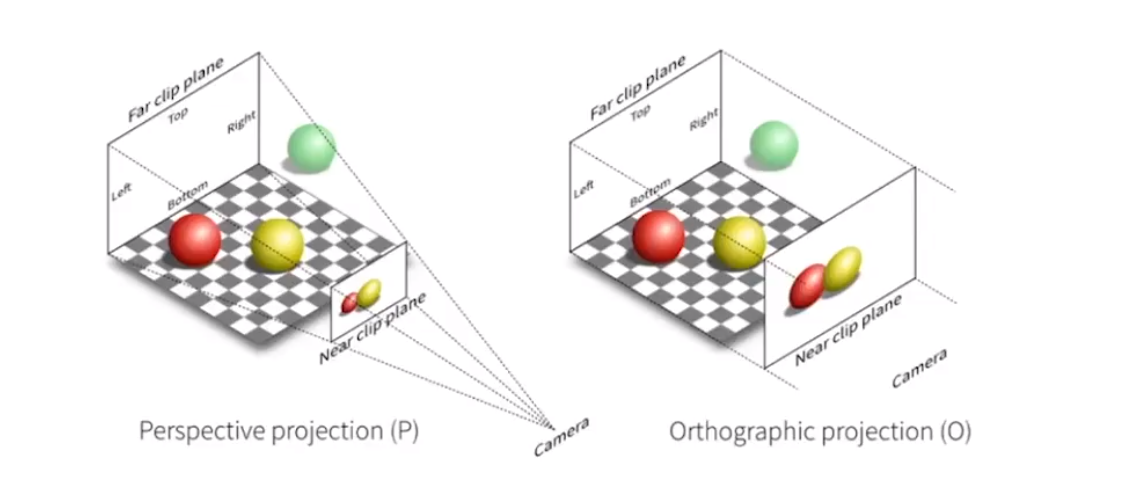
\includegraphics[scale=0.5]{resources/twoProjectionTransformation.png}

              两种投影的本质区别就在于是否有近大远小的现象.

              \begin{itemize}
                \item {
                      正交投影(Orthographic projection) :

                      先定义一个空间中的立方体, 给出三个轴的范围$[l,r]\times[b,t]\times[f,n]$,平移并缩放到标准立方体$[-1,1]^3$

                      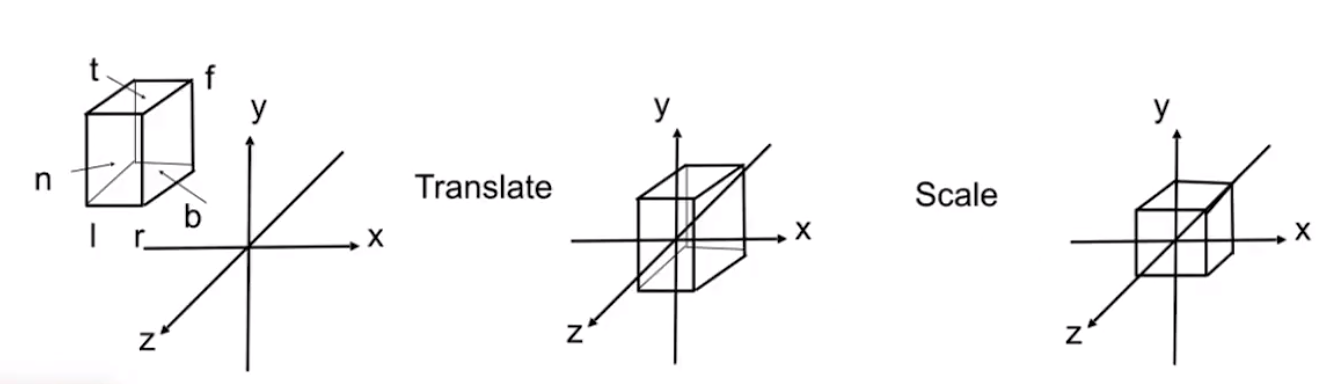
\includegraphics[scale=0.5]{resources/OrthographicProjection.png}

                      矩阵形式为:$$
                        M_{ortho} = \begin{bmatrix}
                          \cfrac{2}{r - l} & 0                & 0                & 0 \\
                          0                & \cfrac{2}{t - b} & 0                & 0 \\
                          0                & 0                & \cfrac{2}{n - f} & 0 \\
                          0                & 0                & 0                & 1
                        \end{bmatrix}
                        \begin{bmatrix}
                          1 & 0 & 0 & -\cfrac{r + l}{2} \\
                          0 & 1 & 0 & -\cfrac{t + b}{2} \\
                          0 & 0 & 1 & -\cfrac{n + f}{2} \\
                          0 & 0 & 0 & 1
                        \end{bmatrix}
                      $$

                      \begin{itemize}
                        \item 注意:由于视线方向沿着-z,所以$n>f$
                        \item 这就是为啥OpenGL用的是左手系
                      \end{itemize}
                      }
                \item {
                      透视变换(Perspective projection) :

                      首先把视锥压缩成长方体.(近平面永远不变,远平面z值不发生变化,中心点不发生变化)$(n \to n,f \to f,M_{persp \to ortho})$

                      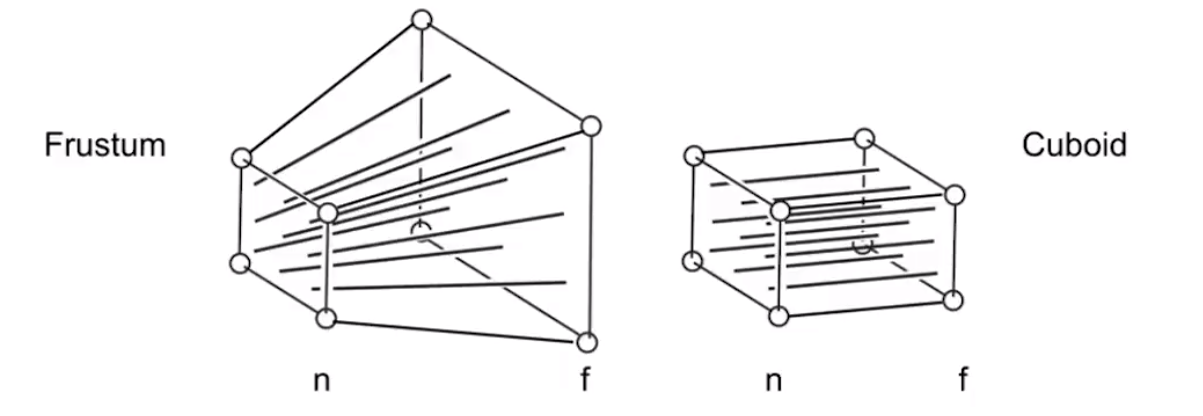
\includegraphics[scale=0.5]{resources/perspectiveProjection.png}

                      关键就在于:要找到中点和被投影对象之间的联系.

                      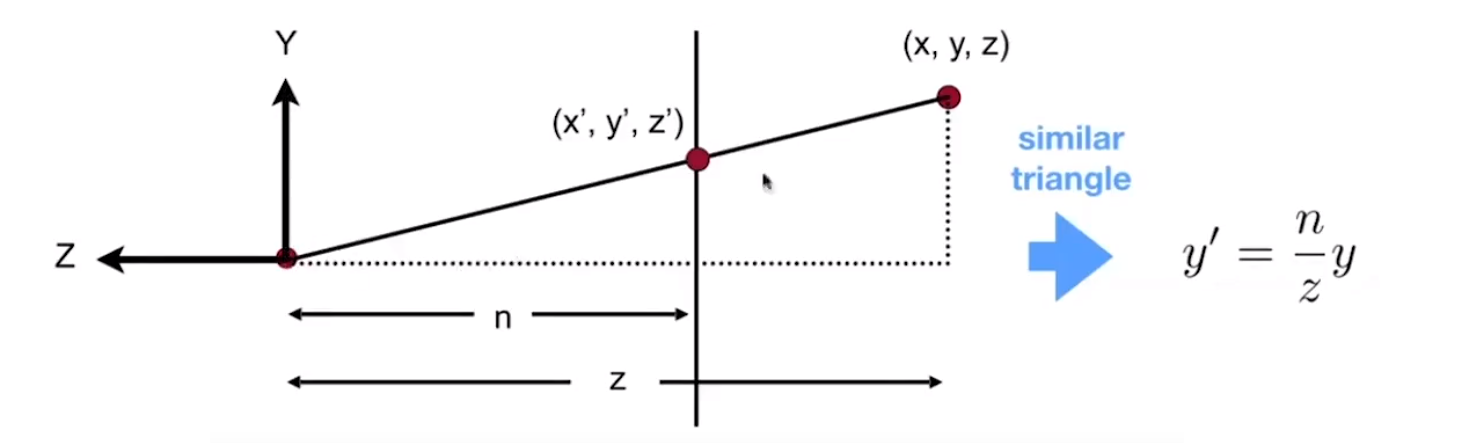
\includegraphics[scale=0.5]{resources/perspectiveProjection_middle.png}

                      $y^\prime = \cfrac{n}{z}y$,由这个公式就可以算出来压缩后的y,并且结果是满足要求的.

                      类似的,还有$x^\prime = \cfrac{n}{z}x$

                      于是得出结论:$$
                        \begin{bmatrix}
                          x \\
                          y \\
                          z \\
                          1
                        \end{bmatrix}
                        \Rightarrow
                        \begin{bmatrix}
                          \cfrac{nx}{z} \\
                          \cfrac{ny}{z} \\
                          unknow        \\
                          1             \\
                        \end{bmatrix}
                        ==
                        \begin{bmatrix}
                          nx           \\
                          ny           \\
                          still unknow \\
                          z
                        \end{bmatrix}
                      $$
                      因此,透视变换的本质就是由目标平面和被投影平面构造一个直角三角形

                      由此写出未完成的投影矩阵 : $$
                        M_{persp \to ortho}
                        =
                        \begin{bmatrix}
                          n & 0 & 0 & 0 \\
                          0 & n & 0 & 0 \\
                          ? & ? & ? & ? \\
                          0 & 0 & 1 & 0
                        \end{bmatrix}
                      $$

                      而这一行未知的也一定与z有关系.

                      另外,任何在目标平面上的点被投影后一定在原地,也就是说:$$
                        \begin{bmatrix}
                          x \\
                          y \\
                          n \\
                          1
                        \end{bmatrix}
                        \Rightarrow
                        \begin{bmatrix}
                          x \\
                          y \\
                          n \\
                          1
                        \end{bmatrix}
                        ==
                        \begin{bmatrix}
                          nx  \\
                          ny  \\
                          n^2 \\
                          n
                        \end{bmatrix}
                      $$

                      仔细思考可以得出:矩阵第三行前两个未知数一定为0:$$
                        \begin{bmatrix}
                          0 & 0 & A & B
                        \end{bmatrix}
                        \begin{bmatrix}
                          x \\
                          y \\
                          n \\
                          1
                        \end{bmatrix}
                        =
                        n^2
                      $$

                      结合另一件事 : 被投影平面上的中心点投影后位置不变,可得出:$$
                        \begin{cases}
                          \begin{bmatrix}
                            0 & 0 & A & B
                          \end{bmatrix}
                          \begin{bmatrix}
                            x \\
                            y \\
                            n \\
                            1
                          \end{bmatrix}
                          =
                          n^2
                          \rightarrow
                          An + B = n^2 \\
                          \begin{bmatrix}
                            0 \\
                            0 \\
                            f \\
                            1
                          \end{bmatrix}
                          \Rightarrow
                          \begin{bmatrix}
                            0 \\
                            0 \\
                            f \\
                            1
                          \end{bmatrix}
                          ==
                          \begin{bmatrix}
                            0   \\
                            0   \\
                            f^2 \\
                            f
                          \end{bmatrix}
                          \rightarrow
                          Af + B = f^2
                        \end{cases}
                        \rightarrow
                        \begin{cases}
                          A = n + f \\
                          B = -nf
                        \end{cases}
                      $$
                      所以 : $$
                        M_{persp \to ortho}
                        =
                        \begin{bmatrix}
                          n & 0 & 0     & 0   \\
                          0 & n & 0     & 0   \\
                          0 & 0 & n + f & -nf \\
                          0 & 0 & 1     & 0
                        \end{bmatrix}
                      $$

                      最后将正交投影和此式结合起来使矩阵变得完整 : $M_{persp} = M_{ortho}M_{persp \to ortho}$
                      }
              \end{itemize}
              }
      \end{itemize}


    }%观测变换结尾

  }%变换结尾

  \subsection{光栅化}{

    \subsubsection{定义与解释}{
      \begin{itemize}
        \item {
              什么是屏幕?
              \begin{itemize}
                \item 对于图形学来说,抽象的认为是一个二维数组,其中每一个元素都是一个像素.
                \item 数组的大小 : 分辨率.
                \item 一个典型的光栅(raster)成像设备.
              \end{itemize}
              }
        \item{
              什么是光栅(raster)?
              \begin{itemize}
                \item raster是德语中"屏幕"的意思.
                \item Rasterize-光栅化 == 把东西画到屏幕上.
              \end{itemize}
              }
        \item{
              像素(Pixel,"picture element"的缩写)是什么?
              \begin{itemize}
                \item 一个很小的只有单个颜色的方块.
                \item 颜色由不同比例的三原色(红绿蓝,rgb)混合而成.
              \end{itemize}
              }
        \item{
              关于"屏幕空间(screen space)"的定义

              \begin{center}
                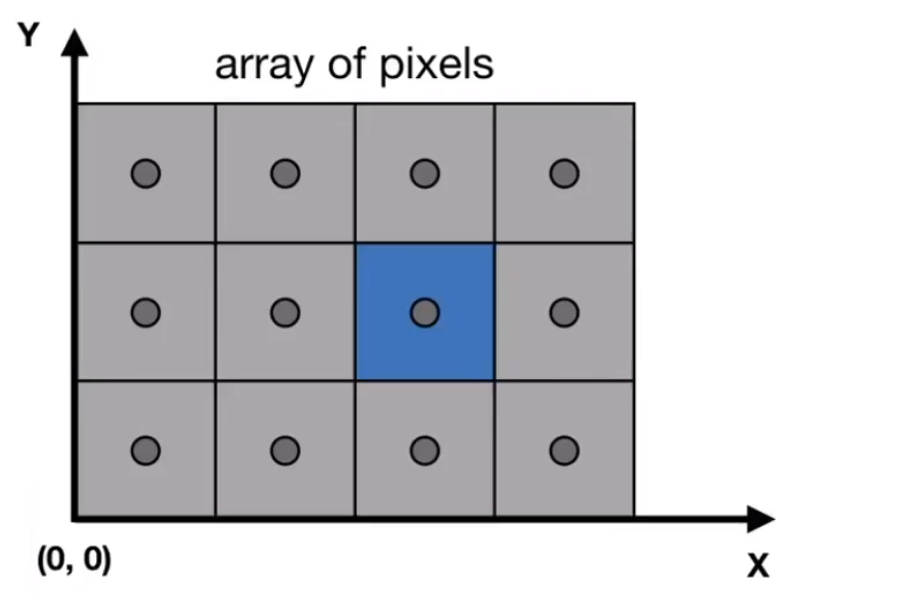
\includegraphics[scale=0.5]{resources/define_of_screen_space_1.png}
              \end{center}

              \begin{itemize}
                \item 认为屏幕的左下角是原点,向上是Y,向右是X.
                \item 像素的坐标都是用$(x,y)$描述的,$x,y$是整数.
                \item 像素的下标范围是从$(0,0)$到$(width - 1,height - 1)$.
                \item 像素的中心总是位于$(x + 0.5,y + 0.5)$.
                \item 屏幕被覆盖到的范围是从$(0,0)$到$(width,height)$(全部铺满).
              \end{itemize}
              }
        \item{
              采样:
              \begin{itemize}
                \item 给定一个函数,在多个地方判断输出结果.
              \end{itemize}
              }
      \end{itemize}
    }%定义与解释结尾

    \subsubsection{三角形光栅化}{
      为什么是三角形?
      \begin{itemize}
        \item 三角形是最基础的多边形.
        \item 任何多边形都可以拆成三角形.
        \item 内部一定是个平面图形.
        \item 内外位置定义清晰
        \item 方便的渐变效果
      \end{itemize}

      将一个三角形光栅化最简单的做法:采样

      采样在图形学中是个重要的概念.此处所指的采样时值对屏幕空间中的像素中心进行采样.(即:判断像素中心是否在函数内,如果是就给像素涂色) :

      \begin{center}
        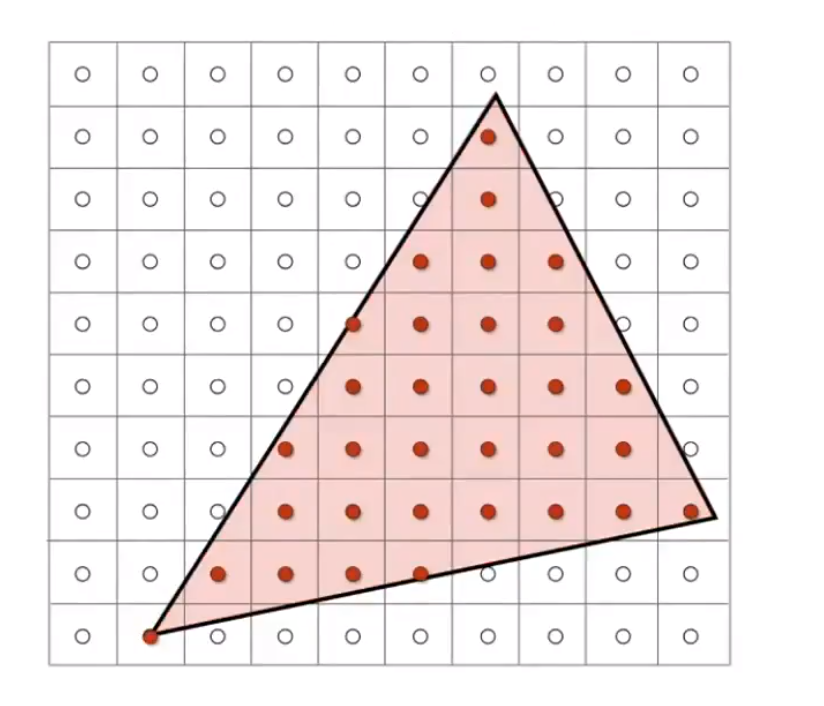
\includegraphics[scale=0.5]{resources/sample_if_each_pixel_inside_triangle.png}
      \end{center}

      代码实现很简单,两层循环遍历屏幕上所有的像素就行.

      要判断一个点是否在三角形内,只需要做叉乘 :

      \begin{center}
        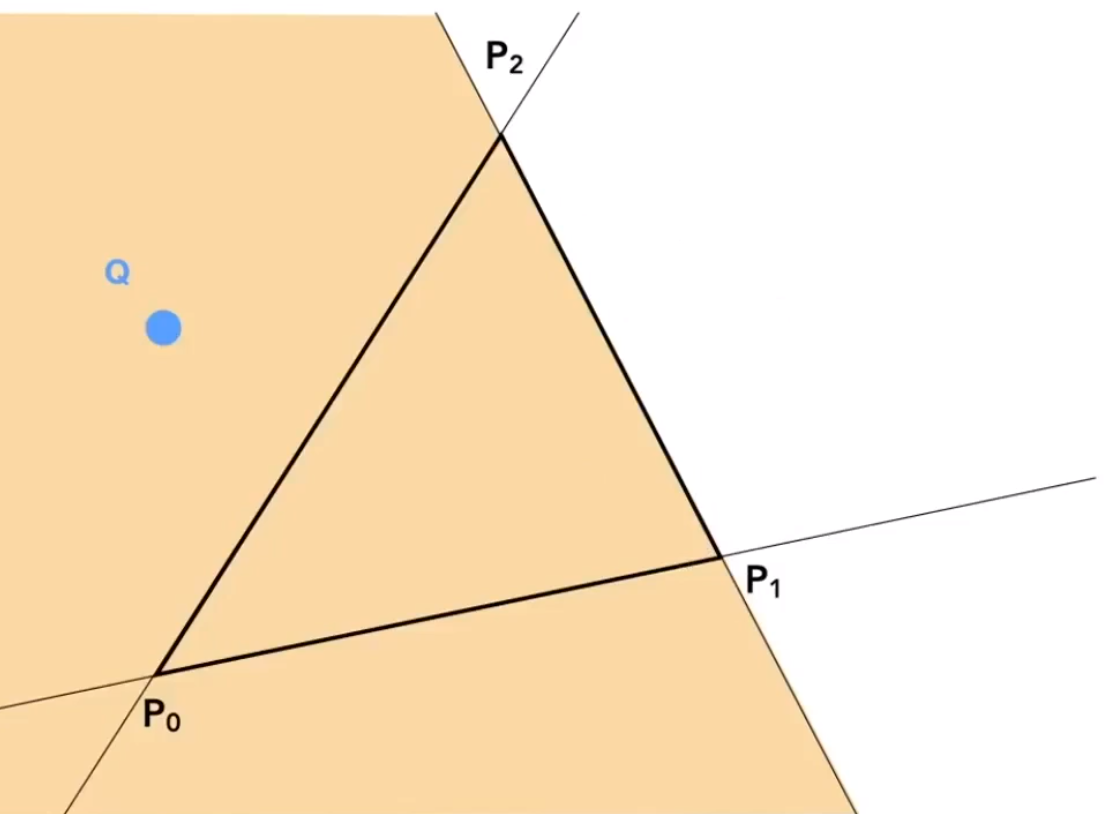
\includegraphics[scale=0.5]{resources/Triangle_Side_Cross_Prodyct.png}
      \end{center}

      比如:
      $$
        \vec{V_1} = \vec{P_1P_2} \times \vec{P_1Q}
      $$

      由于$\vec{V_1}$指向外侧,所以Q在$P_1P_2$左侧

      如此就能不断缩小范围,三条边都判断一次,就能知道该点是否在外面.

      如果点正好在边上,就自己决定.

      但是这么做性能消耗过大,因此可以界定一个判断范围-axis aliged bounding box :

      \begin{center}
        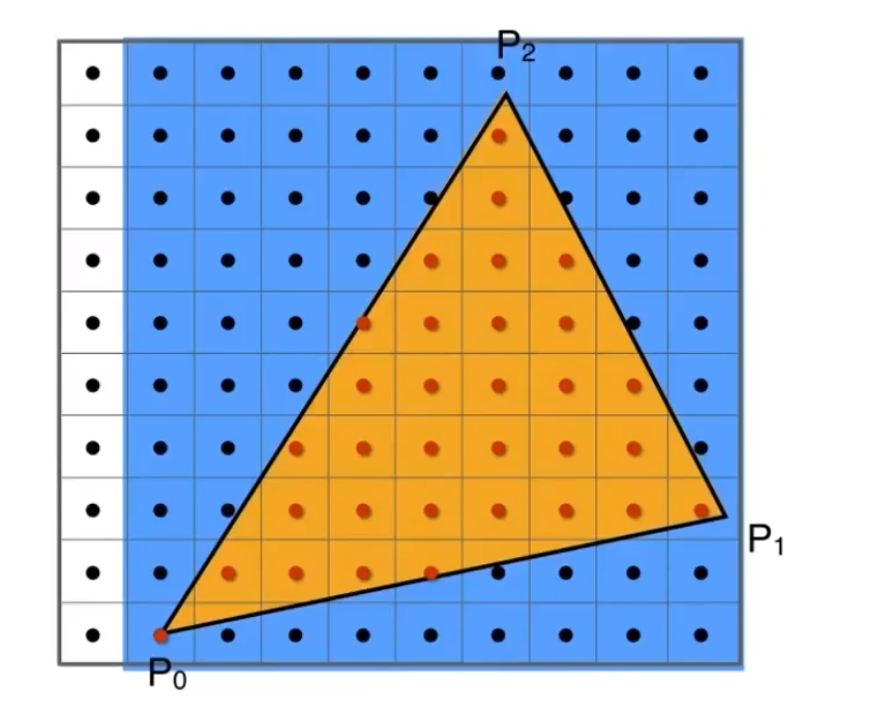
\includegraphics[scale = 0.5]{resources/pixel_boundingBox.png}
      \end{center}

      不过对不同的情况有不同的处理方法,优化方法百花八门,交给数据结构与算法篇吧.
    }%三角形光栅化结尾

  }%光栅化结尾

 }%计算机图形学结尾

}%计算机科学篇结尾
% #TODO Philosophy
% \chapter{哲学}{

\section{逻辑学}{

\subsection{命题公式}{

  \subsubsection{连结词}{

    \begin{itemize}
      \item $P,Q,R,...$表示原子命题(或简单命题)
      \item $1$ 表示命题的真值为真,$0$ 表示命题的真值为假
      \item $\lnot$(非)称为否定连结词.
      \item {
            $\lnot P$称为$P$的否定式 :

            \begin{center}
              \begin{tabular}{c|c}
                \hline
                $P$ & $\lnot P$ \\
                \hline
                $0$ & $1$       \\
                $1$ & $0$       \\
                \hline
              \end{tabular}
            \end{center}

            否定的定义就是取反,如果被连结词是0那么就取1,如果是1那么就取0.
            }
      \item $\land$(与)称为合取连结词
      \item {
            $P \land Q$称为$P$与$Q$的合取式 :

            \begin{center}
              \begin{tabular}{c|c|c}
                \hline
                $P$ & $Q$ & $P \land Q$ \\
                \hline
                0   & 0   & 0           \\
                0   & 1   & 0           \\
                1   & 0   & 0           \\
                1   & 1   & 1           \\
                \hline
              \end{tabular}
            \end{center}

            合取的定义就是只有当两边都是1的时候才取1.

            注意左边两列,可以当成二进制读出"0","1","2","3",此表称为真值表.

            构造真值表的方法就是将所有命题列出,每个命题一列,当有$n$个命题时就会有$2^n$行,从左往右第一个命题二分,一半是0一半是1,第二列在第一列的基础上再次二分$\dots$,如此就能写出所有取值.
            }
      \item $\lor$(或)称为析取连结词
      \item {
            $P \lor Q$称为$P$与$Q$的析取式 :

            \begin{center}
              \begin{tabular}{c|c|c}
                \hline
                $P$ & $Q$ & $P \lor Q$ \\
                \hline
                0   & 0   & 0          \\
                0   & 1   & 1          \\
                1   & 0   & 1          \\
                1   & 1   & 1          \\
                \hline
              \end{tabular}
            \end{center}

            析取的定义就是只有当两边都是0时才取0,否则取1.
            }
      \item $\to$(如果$\dots$则$\dots$)称为蕴涵连结词
      \item {
            $P \to Q$称为$P$与$Q$的蕴涵式 :

            \begin{center}
              \begin{tabular}{c|c|c}
                \hline
                $P$ & $Q$ & $P \to Q$ \\
                \hline
                0   & 0   & 1         \\
                0   & 1   & 1         \\
                1   & 0   & 0         \\
                1   & 1   & 1         \\
              \end{tabular}
            \end{center}

            蕴含的定义就是命题的推导 : 如果$P$是个假命题(0),$Q$也是个假命题(0),那么"P的结论是Q"就是个真命题($P \to Q \Leftrightarrow 1$)

            只考虑形式逻辑不考虑内在联系,因此有局限性,有时候会得到一些奇怪且显然错误的结论.

            可以把它当成$\leq$(?)
            }
      \item $\leftrightarrow$ 称为等价联结词
      \item {
            $P \leftrightarrow Q$称为$P$与$Q$的等价式 :

            \begin{center}
              \begin{tabular}{c|c|c}
                \hline
                $P$ & $Q$ & $P \leftrightarrow Q$ \\
                \hline
                0   & 0   & 1                     \\
                0   & 1   & 0                     \\
                1   & 0   & 0                     \\
                1   & 1   & 1                     \\
                \hline
              \end{tabular}
            \end{center}

            只有当两边命题都是真命题或者假命题的时候才是真.
            }
    \end{itemize}

    联结词优先级为 : $\lnot > (\land \geq \lor) > (\to \geq \leftrightarrow)$(是否取等号看具体定义,默认相等)
  }%联接词结尾

  \subsubsection{命题公式的定义}{
    \begin{enumerate}
      \item 单个命题变元(或常元)($P,Q,R,...$)是命题公式.
      \item 如果$A$是命题公式,则$(\lnot A)$也是.
      \item 如果$A,B$都是命题公式,则$(A \land B),(A \lor B),(A \to B),(A \leftrightarrow B)$也是.
      \item 只有有限次应用$1 - 3$形成的符号串才是命题公式(有限长度).
    \end{enumerate}
  }%命题公式的定义结尾

  \subsubsection{命题公式举例}{
    $P$:简单命题(无连结词)

    $(\lnot(\lnot(\lnot P)))$, $\lnot\lnot\lnot P$:复合命题(有连结词)

    $(P \to (Q \to R))$, $P \to (Q \to R)$:括号不能乱去,此命题是"$P$"的结论是"如果$Q$则$R$".与代数运算类似,如果无括号就从左往右,如果有就优先结合括号.
  }%命题公式举例

  \subsubsection{真值表}{
    将公式可能的赋值全部列出,后面再列出公式的取值,就称为真值表.

    \begin{center}
      \begin{tabular}{c|c|c|c|c}
        \hline
        $P$                       & $Q$      & $P \to Q$                                   & $P \land\lnot P$                            & $P\land(P \lor Q) \leftrightarrow P$ \\
        \hline
        0                         & 0        & 1                                           & 0                                           & 1                                    \\
        0                         & 1        & 1                                           & 0                                           & 1                                    \\
        1                         & 0        & 0                                           & 0                                           & 1                                    \\
        1                         & 1        & 1                                           & 0                                           & 1                                    \\
        \hline
        \multicolumn{2}{c|}{赋值} & 可满足式 & $\underset{\mbox{矛盾式}}{\mbox{(永假式)}}$ & $\underset{\mbox{重言式}}{\mbox{(永真式)}}$
      \end{tabular}
    \end{center}

    \begin{itemize}
      \item 可满足式 : 至少有一种情况可以取值为真.
      \item 矛盾式 : 没有可以取真的情况.
      \item 永真式 : 所有的取值都取真,是可满足式的一种.
    \end{itemize}
  }%真值表

}%命题公式结尾

\subsection{等值演算}{

  \subsubsection{等值式}{
    等值式$A \Leftrightarrow B$的意思就是: $A \leftrightarrow B$是永真式 :

    \begin{center}
      \begin{tabular}{c|c|c|c|c}
        \hline
        $P$ & $Q$ & $P \to Q$ & $\lnot P \lor Q$ & $(P \to Q) \leftrightarrow (\lnot P \lor Q)$ \\
        \hline
        0   & 0   & 1         & 1                & 1                                            \\
        0   & 1   & 1         & 1                & 1                                            \\
        1   & 0   & 0         & 0                & 1                                            \\
        1   & 1   & 1         & 1                & 1                                            \\
        \hline
      \end{tabular}
    \end{center}

    $\therefore P \to Q \Leftrightarrow \lnot P \lor Q$

    意义就在于:证明是等值式后可以将两个公式互相随意替换而不改变运算结果.
  }%等值式结尾

  \subsubsection{基本等值式}{
    \begin{itemize}
      \item 幂等律 : $A \Leftrightarrow A \lor A,A \Leftrightarrow A \land A$
      \item 交换律 : $A \lor B \Leftrightarrow B \lor A,A \land B \Leftrightarrow B \land A$
      \item 结合律 : $(A \lor B) \lor C \Leftrightarrow A \lor (B \lor C),(A \land B) \land C \Leftrightarrow A \land (B \land C)$
      \item 分配律 : $A \land (B \lor C) \Leftrightarrow (A \land B) \lor (A \land C),A \lor (B \land C) \Leftrightarrow (A \lor B) \land (A \lor C)$
      \item 德$\cdot$摩根律 : $\lnot (A \lor B) \Leftrightarrow \lnot A \land \lnot B,\lnot (A \land B) \Leftrightarrow \lnot A \lor \lnot B$
      \item 吸收律 : $A \lor (A \land B) \Leftrightarrow A,A \land (A \lor B) \Leftrightarrow A$
      \item 零律 : $A \lor 1 \Leftrightarrow 1,A \land 0 \Leftrightarrow 0$
      \item 同一律 : $A \lor 0 \Leftrightarrow A,A \land 1 \Leftrightarrow A$
      \item 排中律 : $A \lor \lnot A \Leftrightarrow 1$
      \item 矛盾律 : $A \land \lnot A \Leftrightarrow 0$
      \item 双重否定律 : $\lnot \lnot A \Leftrightarrow A$
      \item 蕴涵等值式 : $A \to B \Leftrightarrow \lnot A \lor B$
      \item 等价等值式 : $A \leftrightarrow B \Leftrightarrow (A \to B) \land (B \to A)$
      \item 等价否定等值式 : $A \leftrightarrow B \Leftrightarrow \lnot A \leftrightarrow \lnot B$
      \item 假言易位 : $A \to B \Leftrightarrow \lnot B \to \lnot A$
      \item 归谬论 : $(A \to B) \land (A \to \lnot B) \Leftrightarrow \lnot A$
      \item 对偶原理 : 一个等值式$\lor - \land$互换,并将结果$0 - 1$互换,那么依然是对的.
      \item 排中律略有争议 : 在某些地方问题并不是非错即对,不过一般默认成立.
      \item 以上公式都可以通过列真值表证明.
    \end{itemize}
  }%基本等值式结尾

  \subsubsection{等值演算}{
    要证明等值式,除了列真值表还可以做等值演算.

    例 :

    \begin{math}
      P \to (Q \to R) \\
      \Leftrightarrow P \to (\lnot Q \lor R)(\mbox{蕴涵等值式,置换规则}) \\
      \Leftrightarrow \lnot P \lor (\lnot Q \lor R) \\
      \Leftrightarrow (\lnot P \lor \lnot Q) \lor R (\mbox{结合律}) \\
      \Leftrightarrow \lnot (P \land Q) \lor R (\mbox{德$\cdot$摩根律}) \\
      \Leftrightarrow (P \land Q) \to R (\mbox{蕴涵等值式})
    \end{math}
  }%等值演算结尾

}%等值演算结尾

\subsection{命题推理逻辑}{

  \subsubsection{推理的形式结构}{
    前提 : $A_1.A_2,\dots,A_K$

    结论 : $B$

    推理的形式结构 : $(A_1 \land A_2 \land \dots \land A_K) \to B$
  }%推理的形式结构结尾

  \subsubsection{重要的推理定律}{
    推理定律-$A \Rightarrow B$(由A可以推出B) : $A \to B$是永真式

    \begin{itemize}
      \item \reasoningStructure{附加律}{$A \Rightarrow (A \lor B)$}{$A$}{$A \lor B$}{$A \to (A \lor B)$}
      \item \reasoningStructure{化简律}{$(A \land B) \Rightarrow A,(A \land B) \Rightarrow B$}{$A \land B$}{}{}
      \item \reasoningStructure{假言推理}{$(A \to B) \land A \Rightarrow B$}{$A \to B,A$}{$B$}{$((A \to B) \land A) \to B$}
      \item \reasoningStructure{拒取式}{$(A \to B) \land \lnot B \Rightarrow \lnot A$}{$A \to B,\lnot B$}{$\lnot A$}{$((A \to B) \land \lnot B) \to (\lnot A)$}
      \item \reasoningStructure{析取三段论}{$(A \lor B) \land \lnot A \Rightarrow B,(A \lor B) \land \lnot B \Rightarrow A$}{$A \lor B,\lnot A$}{$B$}{$((A \lor B)\land \lnot A) \to B$}
      \item \reasoningStructure{假言三段论}{$(A \to B) \land (B \to C) \Rightarrow (A \to C)$}{$A \to B,B \to C$}{$A \to C$}{$((A \to B) \land (B \to C)) \to (A \to C)$}
      \item \reasoningStructure{等价三段论}{$(A \leftrightarrow B) \land (B \leftrightarrow C) \Rightarrow (A \leftrightarrow C)$}{$A \leftrightarrow B,B \leftrightarrow C$}{$A \leftrightarrow C$}{$((A \leftrightarrow B) \land (B \leftrightarrow C)) \to (A \leftrightarrow C)$}
      \item \reasoningStructure{构造性两难}{$(A \to B) \land (C \to D) \land (A \lor C) \Rightarrow (B \lor D)$}{$A \to B,C \to D,A \lor C$}{$B \lor D$}{$(A \to B) \land (C \to D) \land (A \lor C) \to (B \lor D)$}
    \end{itemize}
  }%重要的推理定律结尾

  \subsubsection{判断推理正确的方法}{
    前提 : $P \to (Q \to R),P,Q$

    结论 : $R$

    方法一 : 推理的形式结构(判断是否为永真式).

    方法二 : 从前提推演结论(用前提一步步推结论).
  }%判断推理正确的方法结尾

}%命题推理逻辑结尾

\subsection{一阶谓词逻辑}{
  注释 : 谓词逻辑和命题逻辑不互通.在命题逻辑中最基本的单元是原子命题,无法细分.而在谓词逻辑中还要把命题作为陈述句分为"主语","谓语","宾语".

  \subsubsection{个体}{
    将可以独立存在的课题(具体事务或抽象概念)称为个体或个体词,并用$a,b,c,\dots$表示个体常元,用$x,y,z,\dots$表示个体变元.(个体的函数还是个体,比如 : 设$a,b$是数,f(a,b)可以表示$a$和$b$的运算结果,比如$a + b$,$a \cdot b$等.)

    将个体变元的取值范围称为个体域,个体域可以是有穷或者无穷集合.人们称由宇宙间一切事物组成的个体域为全总个体域.

    通常来说如果没有特别说明那么默认使用全总个体域.
  }%个体结尾

  \subsubsection{谓词}{
    将表示个体性质或彼此之间关系的词称为谓词,常用$F,G,H,\dots$表示谓词常元或者谓词变元,用$F(x)$表示"$x$具有性质$F$",用$F(x,y)$表示"$x$和$y$具有关系$F$".

    例如,若$F(x)$表示"$x$是黑色的",$a$表示黑板,则$F(a)$表示"黑板是黑色的";

    如果$F(x,y)$表示"$x$大于$y$",则$F(5,2)$表示"5大于2".
  }%谓词结尾

  \subsubsection{量词}{
    称表示数量的词为量词.他不是表示具体数量的词,而是表示范围.

    \begin{itemize}
      \item {
            全程量词 :

            全称量词是自然语言中的"所有的","一切的","任意的","每一个"."都"等的统称,用负号"$\forall$"表示.

            用$\forall x$表示个体域里的所有x;

            用$\forall x F(x)$表示个体域里所有的$x$都有性质$F$
            }
      \item {
            存在量词 :

            存在量词是自然语言中的"有一个","至少有一个","存在着","有的"等的统称,用负号"$\exists$"表示

            用$\exists x$表示存在个体域里的$x$;

            用$\exists x F(x)$表示在个体域里存在$x$具有性质$F$.
            }
    \end{itemize}
  }%量词,全称量词结尾

  \subsubsection{命题符号化}{
    一阶逻辑中命题符号化的两个基本公式 :

    \begin{itemize}
      \item {
            个体域中所有有性质$F$的个体都有性质$G$,应符号化为"$\forall x (F(x) \to G(x))$",其中 :

            $F(x)$ : $x$具有性质$F$,$G(x)$ : $x$具有性质$G$.
            }
      \item {
            个体域中存在着有兴致$F$同时有性质$G$的个体,应符号化为"$\exists x (F(x) \land G(x))$",其中 :

            $F(x)$ : $x$具有性质$F$,$G(x)$ : $x$具有性质$G$.
            }
    \end{itemize}

    例子 :
    \begin{enumerate}
      \item {
            人都吃饭 :

            令$F(x)$ : $x$是人,$G(x)$ : $x$吃饭.

            命题符号化为 : $\forall x (F(x) \to G(x))$.
            }
      \item {
            有人喜欢吃糖 :

            令$F(x)$ : $x$是人,$G(x)$ : $x$喜欢吃糖.

            命题符号化为 : $\exists x (F(x) \land G(x))$.
            }
      \item {
            男人都比女人跑得快(这是假命题).

            令$F(x)$ : $x$是男人,$G(y)$ : $y$是女人,$H(x,y)$ : x比y跑的快.

            命题符号化为 : $$
              \forall x (F(x) \to \forall y (G(y) \to H(x,y)))
            $$
            等价形式为 : $$
              \forall x \forall y (F(x) \land G(y) \to H(x,y))
            $$
            }
    \end{enumerate}
  }%命题符号化

  \subsubsection{一阶谓词逻辑公式}{
    一阶谓词逻辑公式也简称为公式,它的形成规则类似于命题逻辑公式,只需加上一条 : 若$A$是公式,则$\forall x A$与$\exists x A$也都是公式.

    在公式$\forall x A$和$\exists x A$中,称$x$为指导变元,称$A$为相应量词的辖域.在$\forall x$和$\exists x$的辖域中,$x$的所有出现都称为是约束出现,$A$中不是约束出现的变元称为自由出现.

    在一阶逻辑中,量词只能作用于个体上,不能作用于谓词上.

    在二阶逻辑中量词可以作用到谓词上.

    例如 : $$
      \forall x (F(x) \to \exists y (G(y) \land H(x,y,z)))
    $$

    其中$\forall x$的辖域为 : $(F(x) \to \exists y (G(y) \land H(x,y,z)))$,

    $\exists y$的辖域为 : $(G(y) \land H(x,y,z))$

    除了$z$是自由出现的变元以外,其他变元都是约束出现的. :
    $$
    \forall \textcolor{blue}{x} (F(\textcolor{blue}{x}) \to \exists y (G(y) \land H(\textcolor{blue}{x},y,z)))
    $$
    $$
    \forall x (F(x) \to \exists \textcolor{blue}{y} (G(\textcolor{blue}{y}) \land H(x,\textcolor{blue}{y},z)))
    $$
    }%一阶谓词逻辑公式结尾

    \subsubsection{解释}{
      对于给定的公式$A$,如果指定$A$的个体域为已知的$D$,并用特定的个体常元取代$A$中的个体常元,用特定函数取代$A$中的函数变元,用特定的谓词取代$A$中的谓词变元,则就构成了$A$的一个解释.

      给定的一个公式$A$可以有多种解释.

      例 : 给定公式$A$为$\forall x (F(x) \to G(x))$,有多种解释 :
      \begin{enumerate}
        \item {
              取个体域为实数集合,$F(x)$ : $x$是有理数,$G(x)$ : $x$能表示成分数 :

              $A$解释为 : "有理数都能表示成分数",这是真命题.
              }
        \item {
              取个体域为全总个体域,$F(x)$ : $x$是人,$G(x)$ : $x$长着黑头发 :

              $A$解释为 : "人都长着黑头发",这是假命题.
              }
      \end{enumerate}
    }%解释结尾

    \subsubsection{永真,永假,可满足,等值式}{
      \begin{itemize}
        \item 若$A$在任何解释下都为真,则称$A$为永真式.
        \item 若$A$在任何解释下都为假,则称$A$为永假式.
        \item 若$A$至少存在一个成真的解释,则称$A$为可满足式.
        \item 若$A \leftrightarrow B$是永真式,则称$A$与$B$是等值的,记为$A \Leftrightarrow B$,并称$A \Leftrightarrow B$为等值式.
      \end{itemize}
    }%永真,永假,可满足,等值式结尾

    \subsubsection{基本等值式}{
      \begin{itemize}
        \item {
              在有限个体域$D = {a_1,a_2,\dots,a_n}$中消去量词等值式 :

              \begin{enumerate}
                \item $\forall x A(x) \Leftrightarrow A(a_1) \land A(a_2) \land \dots \land A(a_n)$
                \item $\exists x A(x) \Leftrightarrow A(a_1) \lor A(a_2) \lor \dots \lor A(a_n)$
              \end{enumerate}
              }
        \item {
              量词否定等值式 :

              \begin{enumerate}
                \item $\lnot\forall x A(x) \Leftrightarrow \exists x \lnot A(x)$
                \item $\lnot\exists x A(x) \Leftrightarrow \forall x \lnot A(x)$
              \end{enumerate}
              }
        \item {
              量词辖域收缩与扩张等值式($B$中不含$x$) :

              \begin{enumerate}
                \item $\forall x (A(x) \lor B) \Leftrightarrow \forall x A(x) \lor B$
                \item $\forall x (A(x) \land B) \Leftrightarrow \forall x A(x) \land B$
                \item $\forall x (A(x) \to B) \Leftrightarrow \exists x A(x) \to B$
                \item $\forall x (B \to A(x)) \Leftrightarrow B \to \forall x A(x)$
                \item $\exists x (A(x) \lor B) \Leftrightarrow \exists x A(x) \lor B$
                \item $\exists x (A(x) \land B) \Leftrightarrow \exists x A(x) \land B$
                \item $\exists x (A(x) \to B) \Leftrightarrow \forall x A(x) \to B$
                \item $\exists x (B \to A(x)) \Leftrightarrow B \to \exists x A(x)$
              \end{enumerate}
              }
        \item {
              量词分配等值式 :

              \begin{enumerate}
                \item {
                      $\forall x (A(x) \land B(x)) \Leftrightarrow \forall x A(x) \land \forall x B(x)$

                      说明 : 全称量词对"$\land$"有分配律,但对"$\lor$"没有.
                      }
                \item {
                      $\exists x (A(x) \lor B(x)) \Leftrightarrow \exists x A(x) \lor \exists x B(x)$

                      说明 : 存在量词对"$\lor$"有分配率,但对"$\land$"没有.
                      }
              \end{enumerate}
              }
      \end{itemize}
    }%基本等值式结尾

    \subsubsection{前束范式}{
      若公式$A$具有形式$Q_1x_1Q_2x_2 \dots Q_kx_kB$,则称$A$为前束范式,其中$Q_i(1 \leq i \leq k)$为$\forall$或者$\exists$,$B$中不含量词.

      求前束范式时用基本等值式和换名规则.

      换名规则 : 将公式$A$中某量词辖域中出现的某个约束出现的个体变元及相应的指导变元$x_i$,都改成公式$A$中没有出现过的$x_j$,所得公式$A\derivative \Leftrightarrow A$

      例 :

      \begin{math}
        \forall x F(x) \lor \lnot\exists x G(x,y) \\
        \Leftrightarrow \forall x F(x) \lor \forall x \lnot G(x,y)\ \mbox{ (量词否定等值式)} \\
        \Leftrightarrow \forall x F(x) \lor \forall z \lnot G(z,y)\ \mbox{ (换名规则)} \\
        \Leftrightarrow \forall x (F(x) \lor \forall z \lnot G(z,y))\ \mbox{ (辖域扩张等值式)} \\
        \Leftrightarrow \forall x \forall z (F(x) \lor \lnot G(z,y))\ \mbox{ (辖域扩张等值式)} \\
        \Leftrightarrow \forall x \forall z (G(z,y) \to F(x))\ \mbox{ (蕴涵等值式)}
      \end{math}
    }%前束范式结尾

    \subsubsection{重要的推理定律}{
      \begin{enumerate}
        \item $\forall x A(x) \lor \forall x B(x) \Rightarrow \forall x (A(x) \lor B(x))$
        \item $\exists x (A(x) \land B(x)) \Rightarrow \exists x A(x) \land \exists x B(x)$
        \item $\forall x (A(x) \to B(x)) \Rightarrow \forall x A(x) \to \forall x B(x)$
        \item $\forall x (A(x) \to B(x)) \Rightarrow \exists x A(x) \to \exists x B(x)$
      \end{enumerate}

      说明 : 以上四条定律是单向的,所以在使用以上四条推理定律时,千万注意,别将他们当作等值式使用.这样会犯错误的.
    }%重要的推理定律

    }%一阶谓词逻辑结尾

    \subsection{充分必要条件}{

      充分必要条件(sufficient and necessary condition)简称为充要条件.

      在逻辑学中:
      \begin{itemize}
        \item 当命题"若P则Q"为真时,P称为Q的充分条件,Q称为P的必要条件.

              因此:

        \item 当命题"若P则Q"与"若Q则P"皆为真时,P是Q的充分必要条件,同时,Q也是P的充分必要条件.
        \item 当命题"若P则Q"为真,而"若Q则P为假时",P是Q的充分不必要条件,Q是P的必要不充分条件,反之亦然.
      \end{itemize}

      \subsubsection{必要条件}{
        P是Q的必要条件,代表"如果P是假,则Q是假"

        以逻辑符号表示:

        $\lnot P \to \lnot Q$

        通过否定后件,得出"如果Q是真,则P是真".

        $Q \to P$
      }%必要条件结尾

      \subsubsection{充分条件}{
        P是Q的充分条件,代表"如果P是真,则Q是真"或"如果Q是假,则P是假".

        以逻辑符号表示:

        $P \to Q$
      }%充分条件结尾

      \subsubsection{必要条件及充分条件}{
        P是Q的充分及必要条件,代表"当且仅当P是真,则Q是真".

        以逻辑符号表示:

        $P \leftrightarrow Q$

        留意$\lnot P \to \lnot Q$可以推出$Q \to P$.

        $(\lnot P \to \lnot Q) \land (P \to Q)$

        $(Q \to P) \land (P \to Q)$

        $P \leftrightarrow Q$
      }%必要条件及充分条件结尾

    }%充分必要条件结尾

  }%逻辑学结尾

}%哲学结尾
% #TODO Physics
% \chapter{物理}{

 }%物理结尾
% #TODO Chemistry
% \part{化学}{

 }%化学结尾
% #TODO Biology
% \part{生物学}{

 }%生物学结尾
% #TODO Medicine
% \chapter{医学}{

 }%医学结尾
% #TODO Artist
% \part{艺术}{

 }%艺术结尾
\end{document}